\documentclass[twoside]{book}

% Packages required by doxygen
\usepackage{fixltx2e}
\usepackage{calc}
\usepackage{doxygen}
\usepackage{graphicx}
\usepackage[utf8]{inputenc}
\usepackage{makeidx}
\usepackage{multicol}
\usepackage{multirow}
\PassOptionsToPackage{warn}{textcomp}
\usepackage{textcomp}
\usepackage[nointegrals]{wasysym}
\usepackage[table]{xcolor}

% Font selection
\usepackage[T1]{fontenc}
\usepackage{mathptmx}
\usepackage[scaled=.90]{helvet}
\usepackage{courier}
\usepackage{amssymb}
\usepackage{sectsty}
\renewcommand{\familydefault}{\sfdefault}
\allsectionsfont{%
  \fontseries{bc}\selectfont%
  \color{darkgray}%
}
\renewcommand{\DoxyLabelFont}{%
  \fontseries{bc}\selectfont%
  \color{darkgray}%
}
\newcommand{\+}{\discretionary{\mbox{\scriptsize$\hookleftarrow$}}{}{}}

% Page & text layout
\usepackage{geometry}
\geometry{%
  a4paper,%
  top=2.5cm,%
  bottom=2.5cm,%
  left=2.5cm,%
  right=2.5cm%
}
\tolerance=750
\hfuzz=15pt
\hbadness=750
\setlength{\emergencystretch}{15pt}
\setlength{\parindent}{0cm}
\setlength{\parskip}{0.2cm}
\makeatletter
\renewcommand{\paragraph}{%
  \@startsection{paragraph}{4}{0ex}{-1.0ex}{1.0ex}{%
    \normalfont\normalsize\bfseries\SS@parafont%
  }%
}
\renewcommand{\subparagraph}{%
  \@startsection{subparagraph}{5}{0ex}{-1.0ex}{1.0ex}{%
    \normalfont\normalsize\bfseries\SS@subparafont%
  }%
}
\makeatother

% Headers & footers
\usepackage{fancyhdr}
\pagestyle{fancyplain}
\fancyhead[LE]{\fancyplain{}{\bfseries\thepage}}
\fancyhead[CE]{\fancyplain{}{}}
\fancyhead[RE]{\fancyplain{}{\bfseries\leftmark}}
\fancyhead[LO]{\fancyplain{}{\bfseries\rightmark}}
\fancyhead[CO]{\fancyplain{}{}}
\fancyhead[RO]{\fancyplain{}{\bfseries\thepage}}
\fancyfoot[LE]{\fancyplain{}{}}
\fancyfoot[CE]{\fancyplain{}{}}
\fancyfoot[RE]{\fancyplain{}{\bfseries\scriptsize Generated on Sun Sep 20 2015 18\+:14\+:25 for Speech recognition library by Doxygen }}
\fancyfoot[LO]{\fancyplain{}{\bfseries\scriptsize Generated on Sun Sep 20 2015 18\+:14\+:25 for Speech recognition library by Doxygen }}
\fancyfoot[CO]{\fancyplain{}{}}
\fancyfoot[RO]{\fancyplain{}{}}
\renewcommand{\footrulewidth}{0.4pt}
\renewcommand{\chaptermark}[1]{%
  \markboth{#1}{}%
}
\renewcommand{\sectionmark}[1]{%
  \markright{\thesection\ #1}%
}

% Indices & bibliography
\usepackage{natbib}
\usepackage[titles]{tocloft}
\setcounter{tocdepth}{3}
\setcounter{secnumdepth}{5}
\makeindex

% Hyperlinks (required, but should be loaded last)
\usepackage{ifpdf}
\ifpdf
  \usepackage[pdftex,pagebackref=true]{hyperref}
\else
  \usepackage[ps2pdf,pagebackref=true]{hyperref}
\fi
\hypersetup{%
  colorlinks=true,%
  linkcolor=blue,%
  citecolor=blue,%
  unicode%
}

% Custom commands
\newcommand{\clearemptydoublepage}{%
  \newpage{\pagestyle{empty}\cleardoublepage}%
}


%===== C O N T E N T S =====

\begin{document}

% Titlepage & ToC
\hypersetup{pageanchor=false,
             bookmarks=true,
             bookmarksnumbered=true,
             pdfencoding=unicode
            }
\pagenumbering{roman}
\begin{titlepage}
\vspace*{7cm}
\begin{center}%
{\Large Speech recognition library \\[1ex]\large 1 }\\
\vspace*{1cm}
{\large Generated by Doxygen 1.8.7}\\
\vspace*{0.5cm}
{\small Sun Sep 20 2015 18:14:25}\\
\end{center}
\end{titlepage}
\clearemptydoublepage
\tableofcontents
\clearemptydoublepage
\pagenumbering{arabic}
\hypersetup{pageanchor=true}

%--- Begin generated contents ---
\chapter{Deprecated List}
\label{deprecated}
\hypertarget{deprecated}{}

\begin{DoxyRefList}
\item[\label{deprecated__deprecated000001}%
\hypertarget{deprecated__deprecated000001}{}%
Member \hyperlink{classspeech_1_1vectorizer_1_1IVectorizer_a63f089697df0617f89e762582e0daef5}{speech\+:\+:vectorizer\+:\+:I\+Vectorizer$<$ Frame\+Type $>$\+:\+:vectorize} (std\+::vector$<$ Frequency\+Sample$<$ Frame\+Type $>$$>$ \&samples)]pass the data source instead \begin{DoxyReturn}{Returns}
the projection of all vectors from given collection  
\end{DoxyReturn}

\item[\label{deprecated__deprecated000002}%
\hypertarget{deprecated__deprecated000002}{}%
Class \hyperlink{classspeech_1_1vectorizer_1_1MaxFrequencyVectorizer}{speech\+:\+:vectorizer\+:\+:Max\+Frequency\+Vectorizer$<$ Frame\+Type $>$} ]
\end{DoxyRefList}
\chapter{Hierarchical Index}
\section{Class Hierarchy}
This inheritance list is sorted roughly, but not completely, alphabetically\+:\begin{DoxyCompactList}
\item \contentsline{section}{speech\+:\+:initializer\+:\+:Abstract\+Gaussian\+Initializer}{\pageref{classspeech_1_1initializer_1_1AbstractGaussianInitializer}}{}
\begin{DoxyCompactList}
\item \contentsline{section}{speech\+:\+:initializer\+:\+:Random\+Initializer}{\pageref{classspeech_1_1initializer_1_1RandomInitializer}}{}
\begin{DoxyCompactList}
\item \contentsline{section}{speech\+:\+:initializer\+:\+:K\+Means\+Initializer}{\pageref{classspeech_1_1initializer_1_1KMeansInitializer}}{}
\end{DoxyCompactList}
\end{DoxyCompactList}
\item \contentsline{section}{C\+V\+Data\+Set}{\pageref{structCVDataSet}}{}
\item \contentsline{section}{speech\+:\+:raw\+\_\+data\+:\+:Data\+Sample$<$ Frame\+Type $>$}{\pageref{classspeech_1_1raw__data_1_1DataSample}}{}
\item \contentsline{section}{speech\+:\+:raw\+\_\+data\+:\+:Data\+Source$<$ Frame\+Type $>$}{\pageref{classspeech_1_1raw__data_1_1DataSource}}{}
\begin{DoxyCompactList}
\item \contentsline{section}{speech\+:\+:raw\+\_\+data\+:\+:Wave\+File\+Data\+Source$<$ Frame\+Type $>$}{\pageref{classspeech_1_1raw__data_1_1WaveFileDataSource}}{}
\end{DoxyCompactList}
\item \contentsline{section}{speech\+:\+:raw\+\_\+data\+:\+:Data\+Source$<$ Frame\+Type $>$\+:\+:data\+Source\+Iterator$<$ data\+Source\+Iterator\+Type $>$}{\pageref{classspeech_1_1raw__data_1_1DataSource_1_1dataSourceIterator}}{}
\item \contentsline{section}{speech\+:\+:raw\+\_\+data\+:\+:Data\+Source$<$ Frame\+Type $>$\+:\+:data\+Source\+Iterator$<$ normal\+Iterator $>$}{\pageref{classspeech_1_1raw__data_1_1DataSource_1_1dataSourceIterator}}{}
\begin{DoxyCompactList}
\item \contentsline{section}{speech\+:\+:raw\+\_\+data\+:\+:Data\+Source$<$ Frame\+Type $>$\+:\+:normal\+Iterator}{\pageref{classspeech_1_1raw__data_1_1DataSource_1_1normalIterator}}{}
\end{DoxyCompactList}
\item \contentsline{section}{speech\+:\+:raw\+\_\+data\+:\+:Data\+Source$<$ Frame\+Type $>$\+:\+:data\+Source\+Iterator$<$ offset\+Iterator $>$}{\pageref{classspeech_1_1raw__data_1_1DataSource_1_1dataSourceIterator}}{}
\begin{DoxyCompactList}
\item \contentsline{section}{speech\+:\+:raw\+\_\+data\+:\+:Data\+Source$<$ Frame\+Type $>$\+:\+:offset\+Iterator}{\pageref{classspeech_1_1raw__data_1_1DataSource_1_1offsetIterator}}{}
\end{DoxyCompactList}
\item exception\begin{DoxyCompactList}
\item \contentsline{section}{speech\+:\+:spelling\+:\+:exception\+:\+:Already\+Built\+Model\+Exception}{\pageref{classspeech_1_1spelling_1_1exception_1_1AlreadyBuiltModelException}}{}
\end{DoxyCompactList}
\item \contentsline{section}{speech\+:\+:raw\+\_\+data\+:\+:filtering\+:\+:Fir\+Filter\+Bank}{\pageref{classspeech_1_1raw__data_1_1filtering_1_1FirFilterBank}}{}
\item \contentsline{section}{speech\+:\+:raw\+\_\+data\+:\+:filtering\+:\+:Fir\+Filter\+Data}{\pageref{structspeech_1_1raw__data_1_1filtering_1_1FirFilterData}}{}
\item \contentsline{section}{speech\+:\+:raw\+\_\+data\+:\+:Frequency\+Sample$<$ Frame\+Type $>$}{\pageref{classspeech_1_1raw__data_1_1FrequencySample}}{}
\item \contentsline{section}{speech\+:\+:H\+M\+M\+Lexicon\+:\+:G\+M\+M\+Likelihood\+Function}{\pageref{classspeech_1_1HMMLexicon_1_1GMMLikelihoodFunction}}{}
\item \contentsline{section}{speech\+:\+:H\+M\+M\+Lexicon}{\pageref{classspeech_1_1HMMLexicon}}{}
\item \contentsline{section}{speech\+:\+:raw\+\_\+data\+:\+:filtering\+:\+:I\+Data\+Sample\+Filter$<$ Frame\+Type $>$}{\pageref{classspeech_1_1raw__data_1_1filtering_1_1IDataSampleFilter}}{}
\begin{DoxyCompactList}
\item \contentsline{section}{speech\+:\+:raw\+\_\+data\+:\+:filtering\+:\+:Emphasis\+Filter$<$ Frame\+Type $>$}{\pageref{classspeech_1_1raw__data_1_1filtering_1_1EmphasisFilter}}{}
\item \contentsline{section}{speech\+:\+:raw\+\_\+data\+:\+:filtering\+:\+:Fir\+Filter$<$ Frame\+Type $>$}{\pageref{classspeech_1_1raw__data_1_1filtering_1_1FirFilter}}{}
\end{DoxyCompactList}
\item \contentsline{section}{speech\+:\+:detector\+:\+:I\+Detector$<$ Frame\+Type $>$}{\pageref{classspeech_1_1detector_1_1IDetector}}{}
\begin{DoxyCompactList}
\item \contentsline{section}{speech\+:\+:detector\+:\+:Naive\+Silence\+Detector$<$ Frame\+Type $>$}{\pageref{classspeech_1_1detector_1_1NaiveSilenceDetector}}{}
\end{DoxyCompactList}
\item \contentsline{section}{speech\+:\+:raw\+\_\+data\+:\+:filtering\+:\+:I\+Frequency\+Sample\+Filter$<$ Frame\+Type $>$}{\pageref{classspeech_1_1raw__data_1_1filtering_1_1IFrequencySampleFilter}}{}
\begin{DoxyCompactList}
\item \contentsline{section}{speech\+:\+:raw\+\_\+data\+:\+:filtering\+:\+:Max\+Frequencies\+Filter$<$ Frame\+Type $>$}{\pageref{classspeech_1_1raw__data_1_1filtering_1_1MaxFrequenciesFilter}}{}
\end{DoxyCompactList}
\item \contentsline{section}{speech\+:\+:transform\+:\+:I\+Frequency\+Transform$<$ Frame\+Type $>$}{\pageref{classspeech_1_1transform_1_1IFrequencyTransform}}{}
\begin{DoxyCompactList}
\item \contentsline{section}{speech\+:\+:transform\+:\+:Discrete\+Fourier\+Transform$<$ Frame\+Type $>$}{\pageref{classspeech_1_1transform_1_1DiscreteFourierTransform}}{}
\item \contentsline{section}{speech\+:\+:transform\+:\+:Fast\+Fourier\+Transform$<$ Frame\+Type $>$}{\pageref{classspeech_1_1transform_1_1FastFourierTransform}}{}
\end{DoxyCompactList}
\item \contentsline{section}{speech\+:\+:metric\+:\+:I\+Metric}{\pageref{classspeech_1_1metric_1_1IMetric}}{}
\begin{DoxyCompactList}
\item \contentsline{section}{speech\+:\+:metric\+:\+:Euclidean\+Distance}{\pageref{classspeech_1_1metric_1_1EuclideanDistance}}{}
\item \contentsline{section}{speech\+:\+:metric\+:\+:Maximum\+Distance}{\pageref{classspeech_1_1metric_1_1MaximumDistance}}{}
\end{DoxyCompactList}
\item \contentsline{section}{speech\+:\+:I\+Stream\+Serializable}{\pageref{classspeech_1_1IStreamSerializable}}{}
\begin{DoxyCompactList}
\item \contentsline{section}{speech\+:\+:clustering\+:\+:I\+Clustering\+Method}{\pageref{classspeech_1_1clustering_1_1IClusteringMethod}}{}
\begin{DoxyCompactList}
\item \contentsline{section}{speech\+:\+:clustering\+:\+:Gaussian\+Mixture\+Model}{\pageref{classspeech_1_1clustering_1_1GaussianMixtureModel}}{}
\item \contentsline{section}{speech\+:\+:clustering\+:\+:K\+Means}{\pageref{classspeech_1_1clustering_1_1KMeans}}{}
\end{DoxyCompactList}
\item \contentsline{section}{speech\+:\+:Language\+Model$<$ Frame\+Type $>$}{\pageref{classspeech_1_1LanguageModel}}{}
\item \contentsline{section}{speech\+:\+:spelling\+:\+:I\+Spelling\+Transcription}{\pageref{classspeech_1_1spelling_1_1ISpellingTranscription}}{}
\begin{DoxyCompactList}
\item \contentsline{section}{speech\+:\+:spelling\+:\+:H\+M\+M}{\pageref{classspeech_1_1spelling_1_1HMM}}{}
\end{DoxyCompactList}
\item \contentsline{section}{speech\+:\+:vectorizer\+:\+:I\+Vectorizer$<$ Frame\+Type $>$}{\pageref{classspeech_1_1vectorizer_1_1IVectorizer}}{}
\begin{DoxyCompactList}
\item \contentsline{section}{speech\+:\+:vectorizer\+:\+:Formant\+Vectorizer$<$ Frame\+Type $>$}{\pageref{classspeech_1_1vectorizer_1_1FormantVectorizer}}{}
\item \contentsline{section}{speech\+:\+:vectorizer\+:\+:Harmonics\+Vectorizer$<$ Frame\+Type $>$}{\pageref{classspeech_1_1vectorizer_1_1HarmonicsVectorizer}}{}
\item \contentsline{section}{speech\+:\+:vectorizer\+:\+:Max\+Frequency\+Vectorizer$<$ Frame\+Type $>$}{\pageref{classspeech_1_1vectorizer_1_1MaxFrequencyVectorizer}}{}
\item \contentsline{section}{speech\+:\+:vectorizer\+:\+:M\+F\+C\+C\+Vectorizer$<$ Frame\+Type $>$}{\pageref{classspeech_1_1vectorizer_1_1MFCCVectorizer}}{}
\item \contentsline{section}{speech\+:\+:vectorizer\+:\+:Thirds\+Power\+Vectorizer$<$ Frame\+Type $>$}{\pageref{classspeech_1_1vectorizer_1_1ThirdsPowerVectorizer}}{}
\end{DoxyCompactList}
\end{DoxyCompactList}
\item length\+\_\+error\begin{DoxyCompactList}
\item \contentsline{section}{speech\+:\+:clustering\+:\+:exception\+:\+:Too\+Less\+Vectors\+Exception}{\pageref{classspeech_1_1clustering_1_1exception_1_1TooLessVectorsException}}{}
\item \contentsline{section}{speech\+:\+:exception\+:\+:Serialization\+Exception}{\pageref{classspeech_1_1exception_1_1SerializationException}}{}
\begin{DoxyCompactList}
\item \contentsline{section}{speech\+:\+:exception\+:\+:Nullptr\+Serialization\+Exception}{\pageref{classspeech_1_1exception_1_1NullptrSerializationException}}{}
\end{DoxyCompactList}
\end{DoxyCompactList}
\item \contentsline{section}{speech\+:\+:vectorizer\+:\+:M\+F\+C\+C\+Vectorizer$<$ Frame\+Type $>$\+:\+:Mel\+Filter}{\pageref{classspeech_1_1vectorizer_1_1MFCCVectorizer_1_1MelFilter}}{}
\item \contentsline{section}{speech\+:\+:H\+M\+M\+Lexicon\+:\+:Multivariate\+Gaussian\+H\+M\+M}{\pageref{classspeech_1_1HMMLexicon_1_1MultivariateGaussianHMM}}{}
\item \contentsline{section}{speech\+:\+:raw\+\_\+data\+:\+:Spectrum}{\pageref{classspeech_1_1raw__data_1_1Spectrum}}{}
\item \contentsline{section}{speech\+:\+:spelling\+:\+:Spelling\+Adjuster}{\pageref{classspeech_1_1spelling_1_1SpellingAdjuster}}{}
\item \contentsline{section}{speech\+:\+:raw\+\_\+data\+:\+:wav\+\_\+header}{\pageref{structspeech_1_1raw__data_1_1wav__header}}{}
\item \contentsline{section}{speech\+:\+:transform\+:\+:window\+:\+:Window}{\pageref{classspeech_1_1transform_1_1window_1_1Window}}{}
\begin{DoxyCompactList}
\item \contentsline{section}{speech\+:\+:transform\+:\+:window\+:\+:Default\+Window}{\pageref{classspeech_1_1transform_1_1window_1_1DefaultWindow}}{}
\item \contentsline{section}{speech\+:\+:transform\+:\+:window\+:\+:Gauss\+Window}{\pageref{classspeech_1_1transform_1_1window_1_1GaussWindow}}{}
\item \contentsline{section}{speech\+:\+:transform\+:\+:window\+:\+:Hamming\+Window}{\pageref{classspeech_1_1transform_1_1window_1_1HammingWindow}}{}
\item \contentsline{section}{speech\+:\+:transform\+:\+:window\+:\+:Hann\+Window}{\pageref{classspeech_1_1transform_1_1window_1_1HannWindow}}{}
\end{DoxyCompactList}
\end{DoxyCompactList}

\chapter{Class Index}
\section{Class List}
Here are the classes, structs, unions and interfaces with brief descriptions\+:\begin{DoxyCompactList}
\item\contentsline{section}{\hyperlink{classspeech_1_1initializer_1_1AbstractGaussianInitializer}{speech\+::initializer\+::\+Abstract\+Gaussian\+Initializer} }{\pageref{classspeech_1_1initializer_1_1AbstractGaussianInitializer}}{}
\item\contentsline{section}{\hyperlink{classspeech_1_1spelling_1_1exception_1_1AlreadyBuiltModelException}{speech\+::spelling\+::exception\+::\+Already\+Built\+Model\+Exception} }{\pageref{classspeech_1_1spelling_1_1exception_1_1AlreadyBuiltModelException}}{}
\item\contentsline{section}{\hyperlink{structCVDataSet}{C\+V\+Data\+Set} }{\pageref{structCVDataSet}}{}
\item\contentsline{section}{\hyperlink{classspeech_1_1raw__data_1_1DataSample}{speech\+::raw\+\_\+data\+::\+Data\+Sample$<$ Frame\+Type $>$} }{\pageref{classspeech_1_1raw__data_1_1DataSample}}{}
\item\contentsline{section}{\hyperlink{classspeech_1_1raw__data_1_1DataSource}{speech\+::raw\+\_\+data\+::\+Data\+Source$<$ Frame\+Type $>$} }{\pageref{classspeech_1_1raw__data_1_1DataSource}}{}
\item\contentsline{section}{\hyperlink{classspeech_1_1raw__data_1_1DataSource_1_1dataSourceIterator}{speech\+::raw\+\_\+data\+::\+Data\+Source$<$ Frame\+Type $>$\+::data\+Source\+Iterator$<$ data\+Source\+Iterator\+Type $>$} }{\pageref{classspeech_1_1raw__data_1_1DataSource_1_1dataSourceIterator}}{}
\item\contentsline{section}{\hyperlink{classspeech_1_1transform_1_1window_1_1DefaultWindow}{speech\+::transform\+::window\+::\+Default\+Window} }{\pageref{classspeech_1_1transform_1_1window_1_1DefaultWindow}}{}
\item\contentsline{section}{\hyperlink{classspeech_1_1transform_1_1DiscreteFourierTransform}{speech\+::transform\+::\+Discrete\+Fourier\+Transform$<$ Frame\+Type $>$} }{\pageref{classspeech_1_1transform_1_1DiscreteFourierTransform}}{}
\item\contentsline{section}{\hyperlink{classspeech_1_1raw__data_1_1filtering_1_1EmphasisFilter}{speech\+::raw\+\_\+data\+::filtering\+::\+Emphasis\+Filter$<$ Frame\+Type $>$} }{\pageref{classspeech_1_1raw__data_1_1filtering_1_1EmphasisFilter}}{}
\item\contentsline{section}{\hyperlink{classspeech_1_1metric_1_1EuclideanDistance}{speech\+::metric\+::\+Euclidean\+Distance} }{\pageref{classspeech_1_1metric_1_1EuclideanDistance}}{}
\item\contentsline{section}{\hyperlink{classspeech_1_1transform_1_1FastFourierTransform}{speech\+::transform\+::\+Fast\+Fourier\+Transform$<$ Frame\+Type $>$} }{\pageref{classspeech_1_1transform_1_1FastFourierTransform}}{}
\item\contentsline{section}{\hyperlink{classspeech_1_1raw__data_1_1filtering_1_1FirFilter}{speech\+::raw\+\_\+data\+::filtering\+::\+Fir\+Filter$<$ Frame\+Type $>$} }{\pageref{classspeech_1_1raw__data_1_1filtering_1_1FirFilter}}{}
\item\contentsline{section}{\hyperlink{classspeech_1_1raw__data_1_1filtering_1_1FirFilterBank}{speech\+::raw\+\_\+data\+::filtering\+::\+Fir\+Filter\+Bank} }{\pageref{classspeech_1_1raw__data_1_1filtering_1_1FirFilterBank}}{}
\item\contentsline{section}{\hyperlink{structspeech_1_1raw__data_1_1filtering_1_1FirFilterData}{speech\+::raw\+\_\+data\+::filtering\+::\+Fir\+Filter\+Data} }{\pageref{structspeech_1_1raw__data_1_1filtering_1_1FirFilterData}}{}
\item\contentsline{section}{\hyperlink{classspeech_1_1vectorizer_1_1FormantVectorizer}{speech\+::vectorizer\+::\+Formant\+Vectorizer$<$ Frame\+Type $>$} }{\pageref{classspeech_1_1vectorizer_1_1FormantVectorizer}}{}
\item\contentsline{section}{\hyperlink{classspeech_1_1raw__data_1_1FrequencySample}{speech\+::raw\+\_\+data\+::\+Frequency\+Sample$<$ Frame\+Type $>$} }{\pageref{classspeech_1_1raw__data_1_1FrequencySample}}{}
\item\contentsline{section}{\hyperlink{classspeech_1_1clustering_1_1GaussianMixtureModel}{speech\+::clustering\+::\+Gaussian\+Mixture\+Model} }{\pageref{classspeech_1_1clustering_1_1GaussianMixtureModel}}{}
\item\contentsline{section}{\hyperlink{classspeech_1_1transform_1_1window_1_1GaussWindow}{speech\+::transform\+::window\+::\+Gauss\+Window} }{\pageref{classspeech_1_1transform_1_1window_1_1GaussWindow}}{}
\item\contentsline{section}{\hyperlink{classspeech_1_1HMMLexicon_1_1GMMLikelihoodFunction}{speech\+::\+H\+M\+M\+Lexicon\+::\+G\+M\+M\+Likelihood\+Function} }{\pageref{classspeech_1_1HMMLexicon_1_1GMMLikelihoodFunction}}{}
\item\contentsline{section}{\hyperlink{classspeech_1_1transform_1_1window_1_1HammingWindow}{speech\+::transform\+::window\+::\+Hamming\+Window} }{\pageref{classspeech_1_1transform_1_1window_1_1HammingWindow}}{}
\item\contentsline{section}{\hyperlink{classspeech_1_1transform_1_1window_1_1HannWindow}{speech\+::transform\+::window\+::\+Hann\+Window} }{\pageref{classspeech_1_1transform_1_1window_1_1HannWindow}}{}
\item\contentsline{section}{\hyperlink{classspeech_1_1vectorizer_1_1HarmonicsVectorizer}{speech\+::vectorizer\+::\+Harmonics\+Vectorizer$<$ Frame\+Type $>$} }{\pageref{classspeech_1_1vectorizer_1_1HarmonicsVectorizer}}{}
\item\contentsline{section}{\hyperlink{classspeech_1_1spelling_1_1HMM}{speech\+::spelling\+::\+H\+M\+M} }{\pageref{classspeech_1_1spelling_1_1HMM}}{}
\item\contentsline{section}{\hyperlink{classspeech_1_1HMMLexicon}{speech\+::\+H\+M\+M\+Lexicon} }{\pageref{classspeech_1_1HMMLexicon}}{}
\item\contentsline{section}{\hyperlink{classspeech_1_1clustering_1_1IClusteringMethod}{speech\+::clustering\+::\+I\+Clustering\+Method} }{\pageref{classspeech_1_1clustering_1_1IClusteringMethod}}{}
\item\contentsline{section}{\hyperlink{classspeech_1_1raw__data_1_1filtering_1_1IDataSampleFilter}{speech\+::raw\+\_\+data\+::filtering\+::\+I\+Data\+Sample\+Filter$<$ Frame\+Type $>$} }{\pageref{classspeech_1_1raw__data_1_1filtering_1_1IDataSampleFilter}}{}
\item\contentsline{section}{\hyperlink{classspeech_1_1detector_1_1IDetector}{speech\+::detector\+::\+I\+Detector$<$ Frame\+Type $>$} }{\pageref{classspeech_1_1detector_1_1IDetector}}{}
\item\contentsline{section}{\hyperlink{classspeech_1_1raw__data_1_1filtering_1_1IFrequencySampleFilter}{speech\+::raw\+\_\+data\+::filtering\+::\+I\+Frequency\+Sample\+Filter$<$ Frame\+Type $>$} }{\pageref{classspeech_1_1raw__data_1_1filtering_1_1IFrequencySampleFilter}}{}
\item\contentsline{section}{\hyperlink{classspeech_1_1transform_1_1IFrequencyTransform}{speech\+::transform\+::\+I\+Frequency\+Transform$<$ Frame\+Type $>$} }{\pageref{classspeech_1_1transform_1_1IFrequencyTransform}}{}
\item\contentsline{section}{\hyperlink{classspeech_1_1metric_1_1IMetric}{speech\+::metric\+::\+I\+Metric} }{\pageref{classspeech_1_1metric_1_1IMetric}}{}
\item\contentsline{section}{\hyperlink{classspeech_1_1spelling_1_1ISpellingTranscription}{speech\+::spelling\+::\+I\+Spelling\+Transcription} }{\pageref{classspeech_1_1spelling_1_1ISpellingTranscription}}{}
\item\contentsline{section}{\hyperlink{classspeech_1_1IStreamSerializable}{speech\+::\+I\+Stream\+Serializable} }{\pageref{classspeech_1_1IStreamSerializable}}{}
\item\contentsline{section}{\hyperlink{classspeech_1_1vectorizer_1_1IVectorizer}{speech\+::vectorizer\+::\+I\+Vectorizer$<$ Frame\+Type $>$} }{\pageref{classspeech_1_1vectorizer_1_1IVectorizer}}{}
\item\contentsline{section}{\hyperlink{classspeech_1_1clustering_1_1KMeans}{speech\+::clustering\+::\+K\+Means} }{\pageref{classspeech_1_1clustering_1_1KMeans}}{}
\item\contentsline{section}{\hyperlink{classspeech_1_1initializer_1_1KMeansInitializer}{speech\+::initializer\+::\+K\+Means\+Initializer} }{\pageref{classspeech_1_1initializer_1_1KMeansInitializer}}{}
\item\contentsline{section}{\hyperlink{classspeech_1_1LanguageModel}{speech\+::\+Language\+Model$<$ Frame\+Type $>$} }{\pageref{classspeech_1_1LanguageModel}}{}
\item\contentsline{section}{\hyperlink{classspeech_1_1raw__data_1_1filtering_1_1MaxFrequenciesFilter}{speech\+::raw\+\_\+data\+::filtering\+::\+Max\+Frequencies\+Filter$<$ Frame\+Type $>$} }{\pageref{classspeech_1_1raw__data_1_1filtering_1_1MaxFrequenciesFilter}}{}
\item\contentsline{section}{\hyperlink{classspeech_1_1vectorizer_1_1MaxFrequencyVectorizer}{speech\+::vectorizer\+::\+Max\+Frequency\+Vectorizer$<$ Frame\+Type $>$} }{\pageref{classspeech_1_1vectorizer_1_1MaxFrequencyVectorizer}}{}
\item\contentsline{section}{\hyperlink{classspeech_1_1metric_1_1MaximumDistance}{speech\+::metric\+::\+Maximum\+Distance} }{\pageref{classspeech_1_1metric_1_1MaximumDistance}}{}
\item\contentsline{section}{\hyperlink{classspeech_1_1vectorizer_1_1MFCCVectorizer_1_1MelFilter}{speech\+::vectorizer\+::\+M\+F\+C\+C\+Vectorizer$<$ Frame\+Type $>$\+::\+Mel\+Filter} }{\pageref{classspeech_1_1vectorizer_1_1MFCCVectorizer_1_1MelFilter}}{}
\item\contentsline{section}{\hyperlink{classspeech_1_1vectorizer_1_1MFCCVectorizer}{speech\+::vectorizer\+::\+M\+F\+C\+C\+Vectorizer$<$ Frame\+Type $>$} }{\pageref{classspeech_1_1vectorizer_1_1MFCCVectorizer}}{}
\item\contentsline{section}{\hyperlink{classspeech_1_1HMMLexicon_1_1MultivariateGaussianHMM}{speech\+::\+H\+M\+M\+Lexicon\+::\+Multivariate\+Gaussian\+H\+M\+M} }{\pageref{classspeech_1_1HMMLexicon_1_1MultivariateGaussianHMM}}{}
\item\contentsline{section}{\hyperlink{classspeech_1_1detector_1_1NaiveSilenceDetector}{speech\+::detector\+::\+Naive\+Silence\+Detector$<$ Frame\+Type $>$} }{\pageref{classspeech_1_1detector_1_1NaiveSilenceDetector}}{}
\item\contentsline{section}{\hyperlink{classspeech_1_1raw__data_1_1DataSource_1_1normalIterator}{speech\+::raw\+\_\+data\+::\+Data\+Source$<$ Frame\+Type $>$\+::normal\+Iterator} }{\pageref{classspeech_1_1raw__data_1_1DataSource_1_1normalIterator}}{}
\item\contentsline{section}{\hyperlink{classspeech_1_1exception_1_1NullptrSerializationException}{speech\+::exception\+::\+Nullptr\+Serialization\+Exception} }{\pageref{classspeech_1_1exception_1_1NullptrSerializationException}}{}
\item\contentsline{section}{\hyperlink{classspeech_1_1raw__data_1_1DataSource_1_1offsetIterator}{speech\+::raw\+\_\+data\+::\+Data\+Source$<$ Frame\+Type $>$\+::offset\+Iterator} }{\pageref{classspeech_1_1raw__data_1_1DataSource_1_1offsetIterator}}{}
\item\contentsline{section}{\hyperlink{classspeech_1_1initializer_1_1RandomInitializer}{speech\+::initializer\+::\+Random\+Initializer} }{\pageref{classspeech_1_1initializer_1_1RandomInitializer}}{}
\item\contentsline{section}{\hyperlink{classspeech_1_1exception_1_1SerializationException}{speech\+::exception\+::\+Serialization\+Exception} }{\pageref{classspeech_1_1exception_1_1SerializationException}}{}
\item\contentsline{section}{\hyperlink{classspeech_1_1raw__data_1_1Spectrum}{speech\+::raw\+\_\+data\+::\+Spectrum} }{\pageref{classspeech_1_1raw__data_1_1Spectrum}}{}
\item\contentsline{section}{\hyperlink{classspeech_1_1spelling_1_1SpellingAdjuster}{speech\+::spelling\+::\+Spelling\+Adjuster} }{\pageref{classspeech_1_1spelling_1_1SpellingAdjuster}}{}
\item\contentsline{section}{\hyperlink{classspeech_1_1vectorizer_1_1ThirdsPowerVectorizer}{speech\+::vectorizer\+::\+Thirds\+Power\+Vectorizer$<$ Frame\+Type $>$} }{\pageref{classspeech_1_1vectorizer_1_1ThirdsPowerVectorizer}}{}
\item\contentsline{section}{\hyperlink{classspeech_1_1clustering_1_1exception_1_1TooLessVectorsException}{speech\+::clustering\+::exception\+::\+Too\+Less\+Vectors\+Exception} }{\pageref{classspeech_1_1clustering_1_1exception_1_1TooLessVectorsException}}{}
\item\contentsline{section}{\hyperlink{structspeech_1_1raw__data_1_1wav__header}{speech\+::raw\+\_\+data\+::wav\+\_\+header} }{\pageref{structspeech_1_1raw__data_1_1wav__header}}{}
\item\contentsline{section}{\hyperlink{classspeech_1_1raw__data_1_1WaveFileDataSource}{speech\+::raw\+\_\+data\+::\+Wave\+File\+Data\+Source$<$ Frame\+Type $>$} }{\pageref{classspeech_1_1raw__data_1_1WaveFileDataSource}}{}
\item\contentsline{section}{\hyperlink{classspeech_1_1transform_1_1window_1_1Window}{speech\+::transform\+::window\+::\+Window} }{\pageref{classspeech_1_1transform_1_1window_1_1Window}}{}
\end{DoxyCompactList}

\chapter{Class Documentation}
\hypertarget{classspeech_1_1initializer_1_1AbstractGaussianInitializer}{\section{speech\+:\+:initializer\+:\+:Abstract\+Gaussian\+Initializer Class Reference}
\label{classspeech_1_1initializer_1_1AbstractGaussianInitializer}\index{speech\+::initializer\+::\+Abstract\+Gaussian\+Initializer@{speech\+::initializer\+::\+Abstract\+Gaussian\+Initializer}}
}


{\ttfamily \#include $<$Abstract\+Gaussian\+Initializer.\+h$>$}

Inheritance diagram for speech\+:\+:initializer\+:\+:Abstract\+Gaussian\+Initializer\+:\begin{figure}[H]
\begin{center}
\leavevmode
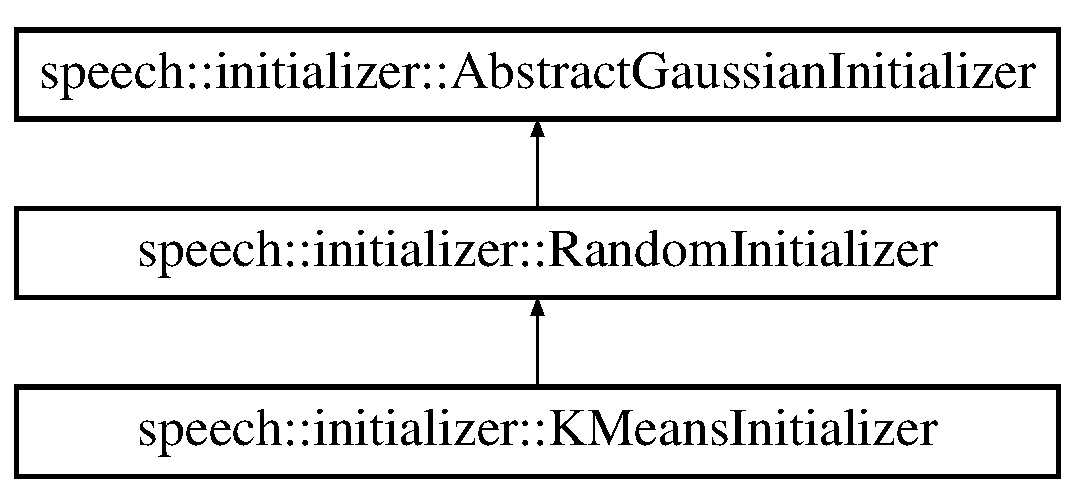
\includegraphics[height=3.000000cm]{classspeech_1_1initializer_1_1AbstractGaussianInitializer}
\end{center}
\end{figure}
\subsection*{Public Member Functions}
\begin{DoxyCompactItemize}
\item 
virtual void \hyperlink{classspeech_1_1initializer_1_1AbstractGaussianInitializer_aa32dc879803a574a9bbd04b9f09f9f79}{initialize} (\hyperlink{classspeech_1_1HMMLexicon_1_1MultivariateGaussianHMM}{speech\+::\+H\+M\+M\+Lexicon\+::\+Multivariate\+Gaussian\+H\+M\+M} \&gaussian\+H\+M\+M)=0
\end{DoxyCompactItemize}


\subsection{Detailed Description}
Initialize the Gaussian H\+M\+M with initial estimates of means and variances 

\subsection{Member Function Documentation}
\hypertarget{classspeech_1_1initializer_1_1AbstractGaussianInitializer_aa32dc879803a574a9bbd04b9f09f9f79}{\index{speech\+::initializer\+::\+Abstract\+Gaussian\+Initializer@{speech\+::initializer\+::\+Abstract\+Gaussian\+Initializer}!initialize@{initialize}}
\index{initialize@{initialize}!speech\+::initializer\+::\+Abstract\+Gaussian\+Initializer@{speech\+::initializer\+::\+Abstract\+Gaussian\+Initializer}}
\subsubsection[{initialize}]{\setlength{\rightskip}{0pt plus 5cm}virtual void speech\+::initializer\+::\+Abstract\+Gaussian\+Initializer\+::initialize (
\begin{DoxyParamCaption}
\item[{{\bf speech\+::\+H\+M\+M\+Lexicon\+::\+Multivariate\+Gaussian\+H\+M\+M} \&}]{gaussian\+H\+M\+M}
\end{DoxyParamCaption}
)\hspace{0.3cm}{\ttfamily [pure virtual]}}}\label{classspeech_1_1initializer_1_1AbstractGaussianInitializer_aa32dc879803a574a9bbd04b9f09f9f79}
Initializes the Gaussians of given H\+M\+M with means and variances 
\begin{DoxyParams}{Parameters}
{\em gaussian\+Hmm} & instance of Gaussian H\+M\+M \\
\hline
\end{DoxyParams}


Implemented in \hyperlink{classspeech_1_1initializer_1_1KMeansInitializer_a300e51ef3bca3d566bffb12f2c6f5924}{speech\+::initializer\+::\+K\+Means\+Initializer}, and \hyperlink{classspeech_1_1initializer_1_1RandomInitializer_a62c031971e30c4c99516a20268511963}{speech\+::initializer\+::\+Random\+Initializer}.



The documentation for this class was generated from the following file\+:\begin{DoxyCompactItemize}
\item 
/home/kacper/\+Projects/speech-\/recognition/src/speech/initializer/Abstract\+Gaussian\+Initializer.\+h\end{DoxyCompactItemize}

\hypertarget{classspeech_1_1spelling_1_1exception_1_1AlreadyBuiltModelException}{\section{speech\+:\+:spelling\+:\+:exception\+:\+:Already\+Built\+Model\+Exception Class Reference}
\label{classspeech_1_1spelling_1_1exception_1_1AlreadyBuiltModelException}\index{speech\+::spelling\+::exception\+::\+Already\+Built\+Model\+Exception@{speech\+::spelling\+::exception\+::\+Already\+Built\+Model\+Exception}}
}
Inheritance diagram for speech\+:\+:spelling\+:\+:exception\+:\+:Already\+Built\+Model\+Exception\+:\begin{figure}[H]
\begin{center}
\leavevmode
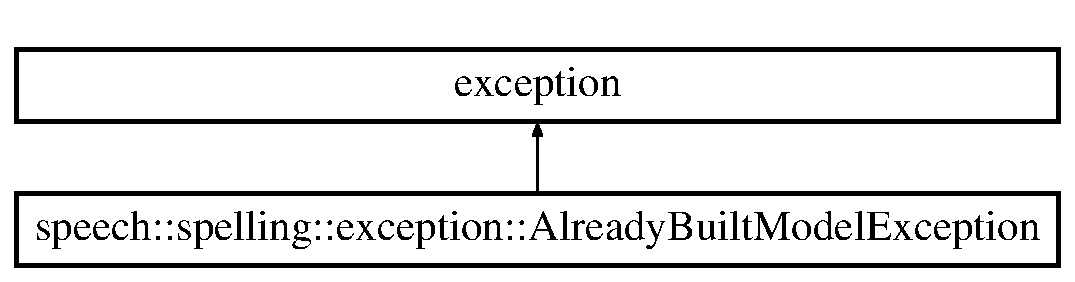
\includegraphics[height=2.000000cm]{classspeech_1_1spelling_1_1exception_1_1AlreadyBuiltModelException}
\end{center}
\end{figure}


The documentation for this class was generated from the following file\+:\begin{DoxyCompactItemize}
\item 
/home/kacper/\+Projects/speech-\/recognition/src/speech/spelling/exception/Already\+Built\+Model\+Exception.\+h\end{DoxyCompactItemize}

\hypertarget{structCVDataSet}{\section{C\+V\+Data\+Set Struct Reference}
\label{structCVDataSet}\index{C\+V\+Data\+Set@{C\+V\+Data\+Set}}
}


{\ttfamily \#include $<$C\+V\+Data\+Set.\+hpp$>$}

\subsection*{Public Types}
\begin{DoxyCompactItemize}
\item 
typedef std\+::multimap\\*
$<$ std\+::string, std\+::string $>$ \hyperlink{structCVDataSet_a1a8ca580cc2dde6a91fb66c82e00b747}{Utterances\+Set}
\item 
typedef std\+::pair$<$ std\+::string, \\*
std\+::string $>$ \hyperlink{structCVDataSet_a39298839ccc861d9828d8fe2d1915110}{Utterance\+Pair}
\end{DoxyCompactItemize}
\subsection*{Public Member Functions}
\begin{DoxyCompactItemize}
\item 
\hypertarget{structCVDataSet_a336a218fba202ee0e0fc55f9bba02f60}{{\bfseries C\+V\+Data\+Set} (const Json\+::\+Value \&root)}\label{structCVDataSet_a336a218fba202ee0e0fc55f9bba02f60}

\item 
\hypertarget{structCVDataSet_a95ee808ec80b03fdee185ac91de59d5a}{void {\bfseries add\+Training\+Utterance} (std\+::string utterance, std\+::string file)}\label{structCVDataSet_a95ee808ec80b03fdee185ac91de59d5a}

\item 
\hypertarget{structCVDataSet_a7050c41cc41f6d9b2a080461c1d049b9}{void {\bfseries add\+Test\+Utterance} (std\+::string utterance, std\+::string file)}\label{structCVDataSet_a7050c41cc41f6d9b2a080461c1d049b9}

\end{DoxyCompactItemize}
\subsection*{Public Attributes}
\begin{DoxyCompactItemize}
\item 
\hyperlink{structCVDataSet_a1a8ca580cc2dde6a91fb66c82e00b747}{Utterances\+Set} \hyperlink{structCVDataSet_ada9a89e03d407ce7e7164ea1327e6f67}{training\+Files}
\item 
\hyperlink{structCVDataSet_a1a8ca580cc2dde6a91fb66c82e00b747}{Utterances\+Set} \hyperlink{structCVDataSet_ad1c35b1bb525b6237f8e15d1f044cd30}{test\+Files}
\item 
std\+::shared\+\_\+ptr\\*
$<$ \hyperlink{classspeech_1_1HMMLexicon}{speech\+::\+H\+M\+M\+Lexicon} $>$ \hyperlink{structCVDataSet_a662cfb97a8b9fbfb9fd7ee1624f418d1}{hmm\+Lexicon}
\end{DoxyCompactItemize}


\subsection{Detailed Description}
A collection of utterances to be used in a cross-\/validation procedure. It is built from a collection of training and test utterances. 

\subsection{Member Typedef Documentation}
\hypertarget{structCVDataSet_a39298839ccc861d9828d8fe2d1915110}{\index{C\+V\+Data\+Set@{C\+V\+Data\+Set}!Utterance\+Pair@{Utterance\+Pair}}
\index{Utterance\+Pair@{Utterance\+Pair}!C\+V\+Data\+Set@{C\+V\+Data\+Set}}
\subsubsection[{Utterance\+Pair}]{\setlength{\rightskip}{0pt plus 5cm}typedef std\+::pair$<$std\+::string, std\+::string$>$ {\bf C\+V\+Data\+Set\+::\+Utterance\+Pair}}}\label{structCVDataSet_a39298839ccc861d9828d8fe2d1915110}
Single utterance file \hypertarget{structCVDataSet_a1a8ca580cc2dde6a91fb66c82e00b747}{\index{C\+V\+Data\+Set@{C\+V\+Data\+Set}!Utterances\+Set@{Utterances\+Set}}
\index{Utterances\+Set@{Utterances\+Set}!C\+V\+Data\+Set@{C\+V\+Data\+Set}}
\subsubsection[{Utterances\+Set}]{\setlength{\rightskip}{0pt plus 5cm}typedef std\+::multimap$<$std\+::string, std\+::string$>$ {\bf C\+V\+Data\+Set\+::\+Utterances\+Set}}}\label{structCVDataSet_a1a8ca580cc2dde6a91fb66c82e00b747}
Collection of utterances 

\subsection{Member Data Documentation}
\hypertarget{structCVDataSet_a662cfb97a8b9fbfb9fd7ee1624f418d1}{\index{C\+V\+Data\+Set@{C\+V\+Data\+Set}!hmm\+Lexicon@{hmm\+Lexicon}}
\index{hmm\+Lexicon@{hmm\+Lexicon}!C\+V\+Data\+Set@{C\+V\+Data\+Set}}
\subsubsection[{hmm\+Lexicon}]{\setlength{\rightskip}{0pt plus 5cm}std\+::shared\+\_\+ptr$<${\bf speech\+::\+H\+M\+M\+Lexicon}$>$ C\+V\+Data\+Set\+::hmm\+Lexicon}}\label{structCVDataSet_a662cfb97a8b9fbfb9fd7ee1624f418d1}
Model created using the training set \hypertarget{structCVDataSet_ad1c35b1bb525b6237f8e15d1f044cd30}{\index{C\+V\+Data\+Set@{C\+V\+Data\+Set}!test\+Files@{test\+Files}}
\index{test\+Files@{test\+Files}!C\+V\+Data\+Set@{C\+V\+Data\+Set}}
\subsubsection[{test\+Files}]{\setlength{\rightskip}{0pt plus 5cm}{\bf Utterances\+Set} C\+V\+Data\+Set\+::test\+Files}}\label{structCVDataSet_ad1c35b1bb525b6237f8e15d1f044cd30}
Utterances used in a test phase \hypertarget{structCVDataSet_ada9a89e03d407ce7e7164ea1327e6f67}{\index{C\+V\+Data\+Set@{C\+V\+Data\+Set}!training\+Files@{training\+Files}}
\index{training\+Files@{training\+Files}!C\+V\+Data\+Set@{C\+V\+Data\+Set}}
\subsubsection[{training\+Files}]{\setlength{\rightskip}{0pt plus 5cm}{\bf Utterances\+Set} C\+V\+Data\+Set\+::training\+Files}}\label{structCVDataSet_ada9a89e03d407ce7e7164ea1327e6f67}
Utterances used in a training phase 

The documentation for this struct was generated from the following file\+:\begin{DoxyCompactItemize}
\item 
/home/kacper/\+Projects/speech-\/recognition/src/C\+V\+Data\+Set.\+hpp\end{DoxyCompactItemize}

\hypertarget{classspeech_1_1raw__data_1_1DataSample}{\section{speech\+:\+:raw\+\_\+data\+:\+:Data\+Sample$<$ Frame\+Type $>$ Class Template Reference}
\label{classspeech_1_1raw__data_1_1DataSample}\index{speech\+::raw\+\_\+data\+::\+Data\+Sample$<$ Frame\+Type $>$@{speech\+::raw\+\_\+data\+::\+Data\+Sample$<$ Frame\+Type $>$}}
}


{\ttfamily \#include $<$Data\+Sample.\+h$>$}

\subsection*{Public Member Functions}
\begin{DoxyCompactItemize}
\item 
\hypertarget{classspeech_1_1raw__data_1_1DataSample_af3f41d2cbd910e6a23453f2f2f2c7cb4}{{\bfseries Data\+Sample} (int \+\_\+size, int \+\_\+length, const std\+::shared\+\_\+ptr$<$ Frame\+Type $>$ \&\+\_\+values)}\label{classspeech_1_1raw__data_1_1DataSample_af3f41d2cbd910e6a23453f2f2f2c7cb4}

\item 
\hypertarget{classspeech_1_1raw__data_1_1DataSample_aab1bd8e721126063be66e7b2e7b3f344}{{\bfseries Data\+Sample} (const \hyperlink{classspeech_1_1raw__data_1_1DataSample}{Data\+Sample}$<$ Frame\+Type $>$ \&ref)}\label{classspeech_1_1raw__data_1_1DataSample_aab1bd8e721126063be66e7b2e7b3f344}

\item 
\hypertarget{classspeech_1_1raw__data_1_1DataSample_a9c6946999fdcc14fccf9729a45e9dd50}{int {\bfseries get\+Size} () const }\label{classspeech_1_1raw__data_1_1DataSample_a9c6946999fdcc14fccf9729a45e9dd50}

\item 
\hypertarget{classspeech_1_1raw__data_1_1DataSample_a221ce8f47f67324f439b492cb81d75b1}{int {\bfseries get\+Length} () const }\label{classspeech_1_1raw__data_1_1DataSample_a221ce8f47f67324f439b492cb81d75b1}

\item 
\hypertarget{classspeech_1_1raw__data_1_1DataSample_a8d0b675c1399dca7a6dbbe9ab9431163}{const std\+::shared\+\_\+ptr$<$ Frame\+Type $>$ {\bfseries get\+Values} () const }\label{classspeech_1_1raw__data_1_1DataSample_a8d0b675c1399dca7a6dbbe9ab9431163}

\end{DoxyCompactItemize}
\subsection*{Protected Attributes}
\begin{DoxyCompactItemize}
\item 
int \hyperlink{classspeech_1_1raw__data_1_1DataSample_a07f56392e007247976f6ab8c2c4edb95}{size}
\item 
int \hyperlink{classspeech_1_1raw__data_1_1DataSample_aeecd9add20856d81b34085090ef19d49}{length}
\item 
\hypertarget{classspeech_1_1raw__data_1_1DataSample_a2b0871621ea7280a83907eecee7d9817}{std\+::shared\+\_\+ptr$<$ Frame\+Type $>$ {\bfseries values}}\label{classspeech_1_1raw__data_1_1DataSample_a2b0871621ea7280a83907eecee7d9817}

\end{DoxyCompactItemize}


\subsection{Detailed Description}
\subsubsection*{template$<$typename Frame\+Type$>$class speech\+::raw\+\_\+data\+::\+Data\+Sample$<$ Frame\+Type $>$}

This class represents a sample of the raw data taken from the data source. It has fixed size and stores digital sound. 

\subsection{Member Data Documentation}
\hypertarget{classspeech_1_1raw__data_1_1DataSample_aeecd9add20856d81b34085090ef19d49}{\index{speech\+::raw\+\_\+data\+::\+Data\+Sample@{speech\+::raw\+\_\+data\+::\+Data\+Sample}!length@{length}}
\index{length@{length}!speech\+::raw\+\_\+data\+::\+Data\+Sample@{speech\+::raw\+\_\+data\+::\+Data\+Sample}}
\subsubsection[{length}]{\setlength{\rightskip}{0pt plus 5cm}template$<$typename Frame\+Type$>$ int {\bf speech\+::raw\+\_\+data\+::\+Data\+Sample}$<$ Frame\+Type $>$\+::length\hspace{0.3cm}{\ttfamily [protected]}}}\label{classspeech_1_1raw__data_1_1DataSample_aeecd9add20856d81b34085090ef19d49}
Length of the sample in milliseconds \hypertarget{classspeech_1_1raw__data_1_1DataSample_a07f56392e007247976f6ab8c2c4edb95}{\index{speech\+::raw\+\_\+data\+::\+Data\+Sample@{speech\+::raw\+\_\+data\+::\+Data\+Sample}!size@{size}}
\index{size@{size}!speech\+::raw\+\_\+data\+::\+Data\+Sample@{speech\+::raw\+\_\+data\+::\+Data\+Sample}}
\subsubsection[{size}]{\setlength{\rightskip}{0pt plus 5cm}template$<$typename Frame\+Type$>$ int {\bf speech\+::raw\+\_\+data\+::\+Data\+Sample}$<$ Frame\+Type $>$\+::size\hspace{0.3cm}{\ttfamily [protected]}}}\label{classspeech_1_1raw__data_1_1DataSample_a07f56392e007247976f6ab8c2c4edb95}
Size of the digital sound sample 

The documentation for this class was generated from the following files\+:\begin{DoxyCompactItemize}
\item 
/home/kacper/\+Projects/speech-\/recognition/src/speech/raw\+\_\+data/Data\+Sample.\+h\item 
/home/kacper/\+Projects/speech-\/recognition/src/speech/raw\+\_\+data/Data\+Sample.\+cpp\end{DoxyCompactItemize}

\hypertarget{classspeech_1_1raw__data_1_1DataSource}{\section{speech\+:\+:raw\+\_\+data\+:\+:Data\+Source$<$ Frame\+Type $>$ Class Template Reference}
\label{classspeech_1_1raw__data_1_1DataSource}\index{speech\+::raw\+\_\+data\+::\+Data\+Source$<$ Frame\+Type $>$@{speech\+::raw\+\_\+data\+::\+Data\+Source$<$ Frame\+Type $>$}}
}


{\ttfamily \#include $<$Data\+Source.\+h$>$}

Inheritance diagram for speech\+:\+:raw\+\_\+data\+:\+:Data\+Source$<$ Frame\+Type $>$\+:\begin{figure}[H]
\begin{center}
\leavevmode
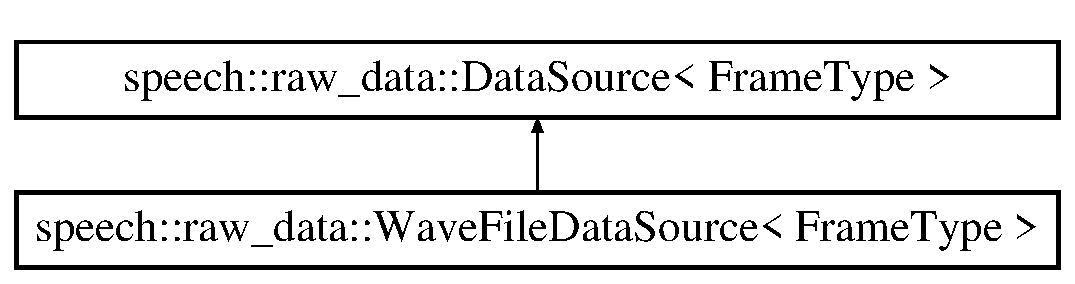
\includegraphics[height=2.000000cm]{classspeech_1_1raw__data_1_1DataSource}
\end{center}
\end{figure}
\subsection*{Classes}
\begin{DoxyCompactItemize}
\item 
class \hyperlink{classspeech_1_1raw__data_1_1DataSource_1_1dataSourceIterator}{data\+Source\+Iterator}
\item 
class \hyperlink{classspeech_1_1raw__data_1_1DataSource_1_1normalIterator}{normal\+Iterator}
\item 
class \hyperlink{classspeech_1_1raw__data_1_1DataSource_1_1offsetIterator}{offset\+Iterator}
\end{DoxyCompactItemize}
\subsection*{Public Member Functions}
\begin{DoxyCompactItemize}
\item 
\hyperlink{classspeech_1_1raw__data_1_1DataSource_a5828f533581fe29765e094dcb2ca6fd5}{Data\+Source} ()
\item 
\hypertarget{classspeech_1_1raw__data_1_1DataSource_ad31cd6f9f9e6527243261bce9255550b}{{\bfseries Data\+Source} (int \hyperlink{classspeech_1_1raw__data_1_1DataSource_a6041f72109ebba9e84e49d71f626b8ea}{sample\+Length})}\label{classspeech_1_1raw__data_1_1DataSource_ad31cd6f9f9e6527243261bce9255550b}

\item 
\hypertarget{classspeech_1_1raw__data_1_1DataSource_a9eaf6b2fb4e0a08be1c755413fce79fa}{virtual void {\bfseries init} ()}\label{classspeech_1_1raw__data_1_1DataSource_a9eaf6b2fb4e0a08be1c755413fce79fa}

\item 
\hypertarget{classspeech_1_1raw__data_1_1DataSource_a87049484c5bdaed0a3cbb744156dc4cc}{virtual void {\bfseries add\+Sample} (\hyperlink{classspeech_1_1raw__data_1_1DataSample}{Data\+Sample}$<$ Frame\+Type $>$ sample)}\label{classspeech_1_1raw__data_1_1DataSource_a87049484c5bdaed0a3cbb744156dc4cc}

\item 
\hypertarget{classspeech_1_1raw__data_1_1DataSource_a3ec31b1ab7642b5cb9db18ca92837e60}{virtual \hyperlink{classspeech_1_1raw__data_1_1DataSource}{Data\+Source}$<$ Frame\+Type $>$\\*
\+::\hyperlink{classspeech_1_1raw__data_1_1DataSource_1_1normalIterator}{normal\+Iterator} {\bfseries get\+Samples\+Iterator\+Begin} ()}\label{classspeech_1_1raw__data_1_1DataSource_a3ec31b1ab7642b5cb9db18ca92837e60}

\item 
\hypertarget{classspeech_1_1raw__data_1_1DataSource_ae0c3a519998215818bc7ae4d03d964db}{virtual \hyperlink{classspeech_1_1raw__data_1_1DataSource}{Data\+Source}$<$ Frame\+Type $>$\\*
\+::\hyperlink{classspeech_1_1raw__data_1_1DataSource_1_1normalIterator}{normal\+Iterator} {\bfseries get\+Samples\+Iterator\+End} ()}\label{classspeech_1_1raw__data_1_1DataSource_ae0c3a519998215818bc7ae4d03d964db}

\item 
\hypertarget{classspeech_1_1raw__data_1_1DataSource_a7cf64445102aa54a7a5e3a3323843cc3}{virtual \hyperlink{classspeech_1_1raw__data_1_1DataSource}{Data\+Source}$<$ Frame\+Type $>$\\*
\+::\hyperlink{classspeech_1_1raw__data_1_1DataSource_1_1offsetIterator}{offset\+Iterator} {\bfseries get\+Offset\+Iterator\+Begin} (int window\+Size\+In\+Milliseconds, int offset\+In\+Milliseconds)}\label{classspeech_1_1raw__data_1_1DataSource_a7cf64445102aa54a7a5e3a3323843cc3}

\item 
\hypertarget{classspeech_1_1raw__data_1_1DataSource_a7dd82ecfd29d317f25f6bf4a032d49b9}{virtual \hyperlink{classspeech_1_1raw__data_1_1DataSource}{Data\+Source}$<$ Frame\+Type $>$\\*
\+::\hyperlink{classspeech_1_1raw__data_1_1DataSource_1_1offsetIterator}{offset\+Iterator} {\bfseries get\+Offset\+Iterator\+End} ()}\label{classspeech_1_1raw__data_1_1DataSource_a7dd82ecfd29d317f25f6bf4a032d49b9}

\end{DoxyCompactItemize}
\subsection*{Protected Member Functions}
\begin{DoxyCompactItemize}
\item 
virtual unsigned int \hyperlink{classspeech_1_1raw__data_1_1DataSource_ab4d9cfbe2d556e6d587e25e4b3074d5f}{get\+Data\+Sample\+Size} (int size\+In\+Milliseconds)=0
\item 
virtual unsigned int \hyperlink{classspeech_1_1raw__data_1_1DataSource_aa4157ef95d70d9c1babd2e9ead0d573a}{get\+Data\+Sample\+Length\+In\+Milliseconds} (int size)=0
\end{DoxyCompactItemize}
\subsection*{Protected Attributes}
\begin{DoxyCompactItemize}
\item 
\hypertarget{classspeech_1_1raw__data_1_1DataSource_a726a703fbc183408d8d1c3e21c3e042c}{std\+::shared\+\_\+ptr$<$ list\\*
$<$ \hyperlink{classspeech_1_1raw__data_1_1DataSample}{Data\+Sample}$<$ Frame\+Type $>$ $>$ $>$ {\bfseries samples}}\label{classspeech_1_1raw__data_1_1DataSource_a726a703fbc183408d8d1c3e21c3e042c}

\item 
int \hyperlink{classspeech_1_1raw__data_1_1DataSource_a6041f72109ebba9e84e49d71f626b8ea}{sample\+Length}
\end{DoxyCompactItemize}


\subsection{Detailed Description}
\subsubsection*{template$<$typename Frame\+Type$>$class speech\+::raw\+\_\+data\+::\+Data\+Source$<$ Frame\+Type $>$}

This abstract class is a base for all data sources used in the application. By data source we define the source of the audio signal. 

\subsection{Constructor \& Destructor Documentation}
\hypertarget{classspeech_1_1raw__data_1_1DataSource_a5828f533581fe29765e094dcb2ca6fd5}{\index{speech\+::raw\+\_\+data\+::\+Data\+Source@{speech\+::raw\+\_\+data\+::\+Data\+Source}!Data\+Source@{Data\+Source}}
\index{Data\+Source@{Data\+Source}!speech\+::raw\+\_\+data\+::\+Data\+Source@{speech\+::raw\+\_\+data\+::\+Data\+Source}}
\subsubsection[{Data\+Source}]{\setlength{\rightskip}{0pt plus 5cm}template$<$typename Frame\+Type$>$ {\bf speech\+::raw\+\_\+data\+::\+Data\+Source}$<$ Frame\+Type $>$\+::{\bf Data\+Source} (
\begin{DoxyParamCaption}
{}
\end{DoxyParamCaption}
)\hspace{0.3cm}{\ttfamily [inline]}}}\label{classspeech_1_1raw__data_1_1DataSource_a5828f533581fe29765e094dcb2ca6fd5}
The default constructor of \hyperlink{classspeech_1_1raw__data_1_1DataSource}{Data\+Source} is here just to have a possibility to declare arrays of such objects 

\subsection{Member Function Documentation}
\hypertarget{classspeech_1_1raw__data_1_1DataSource_aa4157ef95d70d9c1babd2e9ead0d573a}{\index{speech\+::raw\+\_\+data\+::\+Data\+Source@{speech\+::raw\+\_\+data\+::\+Data\+Source}!get\+Data\+Sample\+Length\+In\+Milliseconds@{get\+Data\+Sample\+Length\+In\+Milliseconds}}
\index{get\+Data\+Sample\+Length\+In\+Milliseconds@{get\+Data\+Sample\+Length\+In\+Milliseconds}!speech\+::raw\+\_\+data\+::\+Data\+Source@{speech\+::raw\+\_\+data\+::\+Data\+Source}}
\subsubsection[{get\+Data\+Sample\+Length\+In\+Milliseconds}]{\setlength{\rightskip}{0pt plus 5cm}template$<$typename Frame\+Type$>$ virtual unsigned int {\bf speech\+::raw\+\_\+data\+::\+Data\+Source}$<$ Frame\+Type $>$\+::get\+Data\+Sample\+Length\+In\+Milliseconds (
\begin{DoxyParamCaption}
\item[{int}]{size}
\end{DoxyParamCaption}
)\hspace{0.3cm}{\ttfamily [protected]}, {\ttfamily [pure virtual]}}}\label{classspeech_1_1raw__data_1_1DataSource_aa4157ef95d70d9c1babd2e9ead0d573a}
Returns length of sample with size 'size'. 

Implemented in \hyperlink{classspeech_1_1raw__data_1_1WaveFileDataSource_a62bdc52d91ffeb282da46d42ad3d230c}{speech\+::raw\+\_\+data\+::\+Wave\+File\+Data\+Source$<$ Frame\+Type $>$}.

\hypertarget{classspeech_1_1raw__data_1_1DataSource_ab4d9cfbe2d556e6d587e25e4b3074d5f}{\index{speech\+::raw\+\_\+data\+::\+Data\+Source@{speech\+::raw\+\_\+data\+::\+Data\+Source}!get\+Data\+Sample\+Size@{get\+Data\+Sample\+Size}}
\index{get\+Data\+Sample\+Size@{get\+Data\+Sample\+Size}!speech\+::raw\+\_\+data\+::\+Data\+Source@{speech\+::raw\+\_\+data\+::\+Data\+Source}}
\subsubsection[{get\+Data\+Sample\+Size}]{\setlength{\rightskip}{0pt plus 5cm}template$<$typename Frame\+Type$>$ virtual unsigned int {\bf speech\+::raw\+\_\+data\+::\+Data\+Source}$<$ Frame\+Type $>$\+::get\+Data\+Sample\+Size (
\begin{DoxyParamCaption}
\item[{int}]{size\+In\+Milliseconds}
\end{DoxyParamCaption}
)\hspace{0.3cm}{\ttfamily [protected]}, {\ttfamily [pure virtual]}}}\label{classspeech_1_1raw__data_1_1DataSource_ab4d9cfbe2d556e6d587e25e4b3074d5f}
Returns size of single sample with length 'size\+In\+Milliseconds'. 

Implemented in \hyperlink{classspeech_1_1raw__data_1_1WaveFileDataSource_ac88d8d6a4d6c1f5cf9031fc4d3153542}{speech\+::raw\+\_\+data\+::\+Wave\+File\+Data\+Source$<$ Frame\+Type $>$}.



\subsection{Member Data Documentation}
\hypertarget{classspeech_1_1raw__data_1_1DataSource_a6041f72109ebba9e84e49d71f626b8ea}{\index{speech\+::raw\+\_\+data\+::\+Data\+Source@{speech\+::raw\+\_\+data\+::\+Data\+Source}!sample\+Length@{sample\+Length}}
\index{sample\+Length@{sample\+Length}!speech\+::raw\+\_\+data\+::\+Data\+Source@{speech\+::raw\+\_\+data\+::\+Data\+Source}}
\subsubsection[{sample\+Length}]{\setlength{\rightskip}{0pt plus 5cm}template$<$typename Frame\+Type$>$ int {\bf speech\+::raw\+\_\+data\+::\+Data\+Source}$<$ Frame\+Type $>$\+::sample\+Length\hspace{0.3cm}{\ttfamily [protected]}}}\label{classspeech_1_1raw__data_1_1DataSource_a6041f72109ebba9e84e49d71f626b8ea}
Length of the single sample in milliseconds 

The documentation for this class was generated from the following files\+:\begin{DoxyCompactItemize}
\item 
/home/kacper/\+Projects/speech-\/recognition/src/speech/raw\+\_\+data/Data\+Source.\+h\item 
/home/kacper/\+Projects/speech-\/recognition/src/speech/raw\+\_\+data/Data\+Source.\+cpp\end{DoxyCompactItemize}

\hypertarget{classspeech_1_1raw__data_1_1DataSource_1_1dataSourceIterator}{\section{speech\+:\+:raw\+\_\+data\+:\+:Data\+Source$<$ Frame\+Type $>$\+:\+:data\+Source\+Iterator$<$ data\+Source\+Iterator\+Type $>$ Class Template Reference}
\label{classspeech_1_1raw__data_1_1DataSource_1_1dataSourceIterator}\index{speech\+::raw\+\_\+data\+::\+Data\+Source$<$ Frame\+Type $>$\+::data\+Source\+Iterator$<$ data\+Source\+Iterator\+Type $>$@{speech\+::raw\+\_\+data\+::\+Data\+Source$<$ Frame\+Type $>$\+::data\+Source\+Iterator$<$ data\+Source\+Iterator\+Type $>$}}
}


The documentation for this class was generated from the following file\+:\begin{DoxyCompactItemize}
\item 
/home/kacper/\+Projects/speech-\/recognition/src/speech/raw\+\_\+data/Data\+Source.\+h\end{DoxyCompactItemize}

\hypertarget{classspeech_1_1transform_1_1window_1_1DefaultWindow}{\section{speech\+:\+:transform\+:\+:window\+:\+:Default\+Window Class Reference}
\label{classspeech_1_1transform_1_1window_1_1DefaultWindow}\index{speech\+::transform\+::window\+::\+Default\+Window@{speech\+::transform\+::window\+::\+Default\+Window}}
}
Inheritance diagram for speech\+:\+:transform\+:\+:window\+:\+:Default\+Window\+:\begin{figure}[H]
\begin{center}
\leavevmode
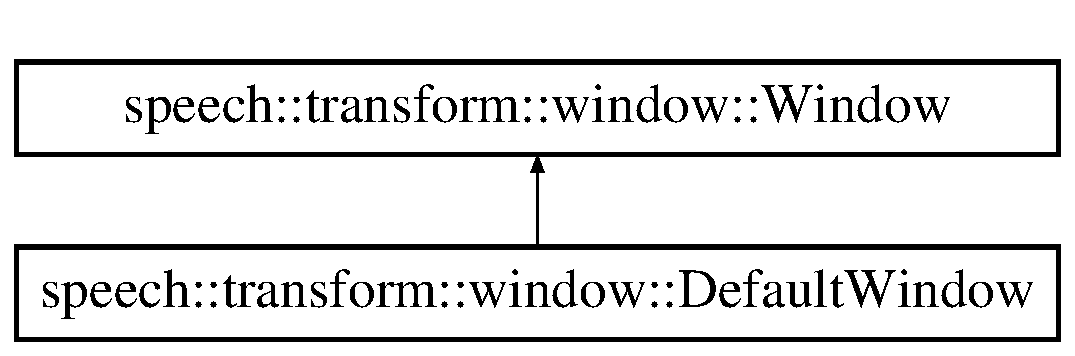
\includegraphics[height=2.000000cm]{classspeech_1_1transform_1_1window_1_1DefaultWindow}
\end{center}
\end{figure}
\subsection*{Static Public Member Functions}
\begin{DoxyCompactItemize}
\item 
\hypertarget{classspeech_1_1transform_1_1window_1_1DefaultWindow_a2c4f779a61c73cc77ce25e3147f05362}{static \hyperlink{classspeech_1_1transform_1_1window_1_1DefaultWindow}{Default\+Window} $\ast$ {\bfseries get\+Instance} ()}\label{classspeech_1_1transform_1_1window_1_1DefaultWindow_a2c4f779a61c73cc77ce25e3147f05362}

\end{DoxyCompactItemize}
\subsection*{Protected Member Functions}
\begin{DoxyCompactItemize}
\item 
\hypertarget{classspeech_1_1transform_1_1window_1_1DefaultWindow_a26e59d18a96737cd2279c8fa638174d6}{virtual const double {\bfseries get\+Window\+Multiplier} (unsigned int index)}\label{classspeech_1_1transform_1_1window_1_1DefaultWindow_a26e59d18a96737cd2279c8fa638174d6}

\end{DoxyCompactItemize}
\subsection*{Additional Inherited Members}


The documentation for this class was generated from the following files\+:\begin{DoxyCompactItemize}
\item 
/home/kacper/\+Projects/speech-\/recognition/src/speech/transform/window/Default\+Window.\+h\item 
/home/kacper/\+Projects/speech-\/recognition/src/speech/transform/window/Default\+Window.\+cpp\end{DoxyCompactItemize}

\hypertarget{classspeech_1_1transform_1_1DiscreteFourierTransform}{\section{speech\+:\+:transform\+:\+:Discrete\+Fourier\+Transform$<$ Frame\+Type $>$ Class Template Reference}
\label{classspeech_1_1transform_1_1DiscreteFourierTransform}\index{speech\+::transform\+::\+Discrete\+Fourier\+Transform$<$ Frame\+Type $>$@{speech\+::transform\+::\+Discrete\+Fourier\+Transform$<$ Frame\+Type $>$}}
}


{\ttfamily \#include $<$Discrete\+Fourier\+Transform.\+h$>$}

Inheritance diagram for speech\+:\+:transform\+:\+:Discrete\+Fourier\+Transform$<$ Frame\+Type $>$\+:\begin{figure}[H]
\begin{center}
\leavevmode
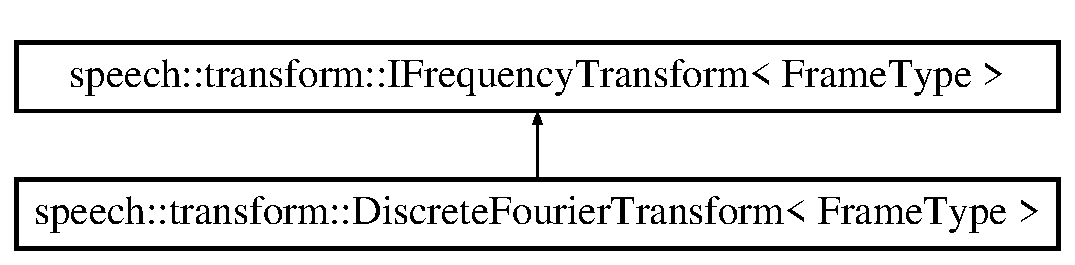
\includegraphics[height=2.000000cm]{classspeech_1_1transform_1_1DiscreteFourierTransform}
\end{center}
\end{figure}
\subsection*{Public Member Functions}
\begin{DoxyCompactItemize}
\item 
\hypertarget{classspeech_1_1transform_1_1DiscreteFourierTransform_adf478699abd139e4cb3ac83e86f6b058}{virtual \hyperlink{classspeech_1_1raw__data_1_1FrequencySample}{Frequency\+Sample}\\*
$<$ Frame\+Type $>$ {\bfseries transform} (const \hyperlink{classspeech_1_1raw__data_1_1DataSample}{Data\+Sample}$<$ Frame\+Type $>$ \&vector)}\label{classspeech_1_1transform_1_1DiscreteFourierTransform_adf478699abd139e4cb3ac83e86f6b058}

\item 
\hypertarget{classspeech_1_1transform_1_1DiscreteFourierTransform_a106bcc8c2399a69a60e15dd90f222c35}{virtual \hyperlink{classspeech_1_1raw__data_1_1DataSample}{Data\+Sample}$<$ Frame\+Type $>$ {\bfseries reverse\+Transform} (const \hyperlink{classspeech_1_1raw__data_1_1FrequencySample}{Frequency\+Sample}$<$ Frame\+Type $>$ \&vector)}\label{classspeech_1_1transform_1_1DiscreteFourierTransform_a106bcc8c2399a69a60e15dd90f222c35}

\item 
\hypertarget{classspeech_1_1transform_1_1DiscreteFourierTransform_a3db5d48847f7f79afb71f993f7502d9f}{virtual \hyperlink{classspeech_1_1raw__data_1_1FrequencySample}{Frequency\+Sample}\\*
$<$ Frame\+Type $>$ {\bfseries transform} (const \hyperlink{classspeech_1_1raw__data_1_1DataSample}{Data\+Sample}$<$ Frame\+Type $>$ \&vector, \hyperlink{classspeech_1_1transform_1_1window_1_1Window}{Window} $\ast$window)}\label{classspeech_1_1transform_1_1DiscreteFourierTransform_a3db5d48847f7f79afb71f993f7502d9f}

\end{DoxyCompactItemize}


\subsection{Detailed Description}
\subsubsection*{template$<$typename Frame\+Type$>$class speech\+::transform\+::\+Discrete\+Fourier\+Transform$<$ Frame\+Type $>$}

Standard Discrete Fourier Transform with the complexity O(n$^\wedge$2) 

The documentation for this class was generated from the following files\+:\begin{DoxyCompactItemize}
\item 
/home/kacper/\+Projects/speech-\/recognition/src/speech/transform/Discrete\+Fourier\+Transform.\+h\item 
/home/kacper/\+Projects/speech-\/recognition/src/speech/transform/Discrete\+Fourier\+Transform.\+cpp\end{DoxyCompactItemize}

\hypertarget{classspeech_1_1raw__data_1_1filtering_1_1EmphasisFilter}{\section{speech\+:\+:raw\+\_\+data\+:\+:filtering\+:\+:Emphasis\+Filter$<$ Frame\+Type $>$ Class Template Reference}
\label{classspeech_1_1raw__data_1_1filtering_1_1EmphasisFilter}\index{speech\+::raw\+\_\+data\+::filtering\+::\+Emphasis\+Filter$<$ Frame\+Type $>$@{speech\+::raw\+\_\+data\+::filtering\+::\+Emphasis\+Filter$<$ Frame\+Type $>$}}
}


{\ttfamily \#include $<$Emphasis\+Filter.\+h$>$}

Inheritance diagram for speech\+:\+:raw\+\_\+data\+:\+:filtering\+:\+:Emphasis\+Filter$<$ Frame\+Type $>$\+:\begin{figure}[H]
\begin{center}
\leavevmode
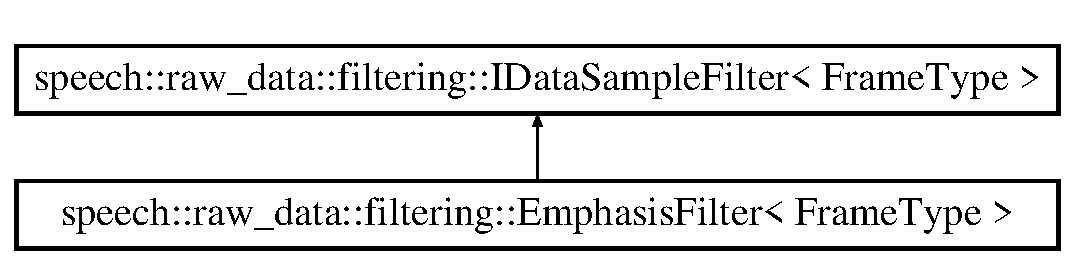
\includegraphics[height=2.000000cm]{classspeech_1_1raw__data_1_1filtering_1_1EmphasisFilter}
\end{center}
\end{figure}
\subsection*{Public Member Functions}
\begin{DoxyCompactItemize}
\item 
\hyperlink{classspeech_1_1raw__data_1_1filtering_1_1EmphasisFilter_a128b508047206178272d05d8e834bbef}{Emphasis\+Filter} (double alpha)
\item 
\hypertarget{classspeech_1_1raw__data_1_1filtering_1_1EmphasisFilter_a822e28df9a52d5dea97a1f27eabfd7d1}{virtual \hyperlink{classspeech_1_1raw__data_1_1DataSample}{Data\+Sample}$<$ Frame\+Type $>$ {\bfseries filter} (const \hyperlink{classspeech_1_1raw__data_1_1DataSample}{Data\+Sample}$<$ Frame\+Type $>$ \&sample)}\label{classspeech_1_1raw__data_1_1filtering_1_1EmphasisFilter_a822e28df9a52d5dea97a1f27eabfd7d1}

\end{DoxyCompactItemize}


\subsection{Detailed Description}
\subsubsection*{template$<$typename Frame\+Type$>$class speech\+::raw\+\_\+data\+::filtering\+::\+Emphasis\+Filter$<$ Frame\+Type $>$}

This filter boosts the amount of energy in the high frequencies. \begin{DoxySeeAlso}{See also}
\href{http://webapp.etsi.org/workprogram/Report_WorkItem.asp?wki_id=18820}{\tt http\+://webapp.\+etsi.\+org/workprogram/\+Report\+\_\+\+Work\+Item.\+asp?wki\+\_\+id=18820} 
\end{DoxySeeAlso}


\subsection{Constructor \& Destructor Documentation}
\hypertarget{classspeech_1_1raw__data_1_1filtering_1_1EmphasisFilter_a128b508047206178272d05d8e834bbef}{\index{speech\+::raw\+\_\+data\+::filtering\+::\+Emphasis\+Filter@{speech\+::raw\+\_\+data\+::filtering\+::\+Emphasis\+Filter}!Emphasis\+Filter@{Emphasis\+Filter}}
\index{Emphasis\+Filter@{Emphasis\+Filter}!speech\+::raw\+\_\+data\+::filtering\+::\+Emphasis\+Filter@{speech\+::raw\+\_\+data\+::filtering\+::\+Emphasis\+Filter}}
\subsubsection[{Emphasis\+Filter}]{\setlength{\rightskip}{0pt plus 5cm}template$<$typename Frame\+Type $>$ {\bf speech\+::raw\+\_\+data\+::filtering\+::\+Emphasis\+Filter}$<$ Frame\+Type $>$\+::{\bf Emphasis\+Filter} (
\begin{DoxyParamCaption}
\item[{double}]{alpha}
\end{DoxyParamCaption}
)\hspace{0.3cm}{\ttfamily [inline]}}}\label{classspeech_1_1raw__data_1_1filtering_1_1EmphasisFilter_a128b508047206178272d05d8e834bbef}
Creates a filter instance with provided weight of the each previous sample, which will be substracted from current sample to emphasise the difference between them\+: u\mbox{[}n\mbox{]} = u\mbox{[}n\mbox{]} -\/ alpha $\ast$ u\mbox{[}n-\/1\mbox{]} 
\begin{DoxyParams}{Parameters}
{\em alpha} & weight of the previous sample \\
\hline
\end{DoxyParams}


The documentation for this class was generated from the following files\+:\begin{DoxyCompactItemize}
\item 
/home/kacper/\+Projects/speech-\/recognition/src/speech/raw\+\_\+data/filtering/Emphasis\+Filter.\+h\item 
/home/kacper/\+Projects/speech-\/recognition/src/speech/raw\+\_\+data/filtering/Emphasis\+Filter.\+cpp\end{DoxyCompactItemize}

\hypertarget{classspeech_1_1metric_1_1EuclideanDistance}{\section{speech\+:\+:metric\+:\+:Euclidean\+Distance Class Reference}
\label{classspeech_1_1metric_1_1EuclideanDistance}\index{speech\+::metric\+::\+Euclidean\+Distance@{speech\+::metric\+::\+Euclidean\+Distance}}
}


{\ttfamily \#include $<$Euclidean\+Distance.\+h$>$}

Inheritance diagram for speech\+:\+:metric\+:\+:Euclidean\+Distance\+:\begin{figure}[H]
\begin{center}
\leavevmode
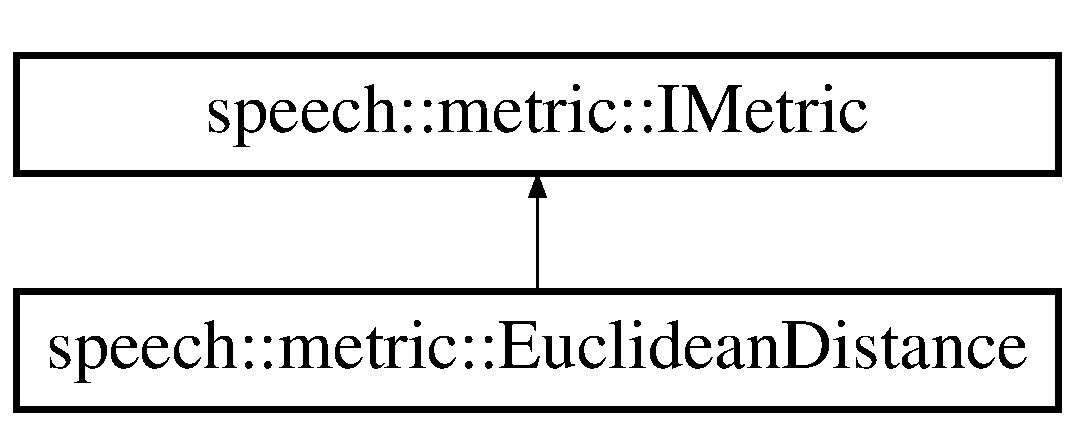
\includegraphics[height=2.000000cm]{classspeech_1_1metric_1_1EuclideanDistance}
\end{center}
\end{figure}
\subsection*{Public Member Functions}
\begin{DoxyCompactItemize}
\item 
virtual double \hyperlink{classspeech_1_1metric_1_1EuclideanDistance_abd0d73ebf83dc218ab8f6ab5dee47064}{operator()} (const std\+::valarray$<$ double $>$ \&v1, const std\+::valarray$<$ double $>$ \&v2) override
\end{DoxyCompactItemize}


\subsection{Detailed Description}
Calculates standard Euclidean distance between two vectors. 

\subsection{Member Function Documentation}
\hypertarget{classspeech_1_1metric_1_1EuclideanDistance_abd0d73ebf83dc218ab8f6ab5dee47064}{\index{speech\+::metric\+::\+Euclidean\+Distance@{speech\+::metric\+::\+Euclidean\+Distance}!operator()@{operator()}}
\index{operator()@{operator()}!speech\+::metric\+::\+Euclidean\+Distance@{speech\+::metric\+::\+Euclidean\+Distance}}
\subsubsection[{operator()}]{\setlength{\rightskip}{0pt plus 5cm}double speech\+::metric\+::\+Euclidean\+Distance\+::operator() (
\begin{DoxyParamCaption}
\item[{const std\+::valarray$<$ double $>$ \&}]{v1, }
\item[{const std\+::valarray$<$ double $>$ \&}]{v2}
\end{DoxyParamCaption}
)\hspace{0.3cm}{\ttfamily [override]}, {\ttfamily [virtual]}}}\label{classspeech_1_1metric_1_1EuclideanDistance_abd0d73ebf83dc218ab8f6ab5dee47064}
Calculates a distance between two vectors. \begin{DoxyReturn}{Returns}
a distance 
\end{DoxyReturn}


Implements \hyperlink{classspeech_1_1metric_1_1IMetric_af15c579c0870b67e862945b6918bc14e}{speech\+::metric\+::\+I\+Metric}.



The documentation for this class was generated from the following files\+:\begin{DoxyCompactItemize}
\item 
/home/kacper/\+Projects/speech-\/recognition/src/speech/metric/Euclidean\+Distance.\+h\item 
/home/kacper/\+Projects/speech-\/recognition/src/speech/metric/Euclidean\+Distance.\+cpp\end{DoxyCompactItemize}

\hypertarget{classspeech_1_1transform_1_1FastFourierTransform}{\section{speech\+:\+:transform\+:\+:Fast\+Fourier\+Transform$<$ Frame\+Type $>$ Class Template Reference}
\label{classspeech_1_1transform_1_1FastFourierTransform}\index{speech\+::transform\+::\+Fast\+Fourier\+Transform$<$ Frame\+Type $>$@{speech\+::transform\+::\+Fast\+Fourier\+Transform$<$ Frame\+Type $>$}}
}


{\ttfamily \#include $<$Fast\+Fourier\+Transform.\+h$>$}

Inheritance diagram for speech\+:\+:transform\+:\+:Fast\+Fourier\+Transform$<$ Frame\+Type $>$\+:\begin{figure}[H]
\begin{center}
\leavevmode
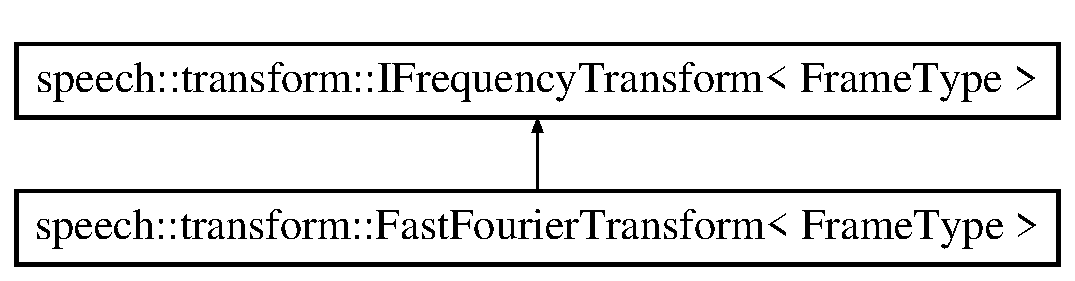
\includegraphics[height=2.000000cm]{classspeech_1_1transform_1_1FastFourierTransform}
\end{center}
\end{figure}
\subsection*{Public Member Functions}
\begin{DoxyCompactItemize}
\item 
\hypertarget{classspeech_1_1transform_1_1FastFourierTransform_ae41aa58b3e4791f5ad8301c766d49d07}{virtual \hyperlink{classspeech_1_1raw__data_1_1FrequencySample}{Frequency\+Sample}\\*
$<$ Frame\+Type $>$ {\bfseries transform} (const \hyperlink{classspeech_1_1raw__data_1_1DataSample}{Data\+Sample}$<$ Frame\+Type $>$ \&vector)}\label{classspeech_1_1transform_1_1FastFourierTransform_ae41aa58b3e4791f5ad8301c766d49d07}

\item 
\hypertarget{classspeech_1_1transform_1_1FastFourierTransform_a34e2dfc18a51fd33a807b8f8c829d912}{virtual \hyperlink{classspeech_1_1raw__data_1_1FrequencySample}{Frequency\+Sample}\\*
$<$ Frame\+Type $>$ {\bfseries transform} (const \hyperlink{classspeech_1_1raw__data_1_1DataSample}{Data\+Sample}$<$ Frame\+Type $>$ \&vector, \hyperlink{classspeech_1_1transform_1_1window_1_1Window}{Window} $\ast$window)}\label{classspeech_1_1transform_1_1FastFourierTransform_a34e2dfc18a51fd33a807b8f8c829d912}

\item 
\hypertarget{classspeech_1_1transform_1_1FastFourierTransform_a0d6f84abf032495e9bbade561b3e8c5f}{virtual \hyperlink{classspeech_1_1raw__data_1_1DataSample}{Data\+Sample}$<$ Frame\+Type $>$ {\bfseries reverse\+Transform} (const \hyperlink{classspeech_1_1raw__data_1_1FrequencySample}{Frequency\+Sample}$<$ Frame\+Type $>$ \&vector)}\label{classspeech_1_1transform_1_1FastFourierTransform_a0d6f84abf032495e9bbade561b3e8c5f}

\end{DoxyCompactItemize}
\subsection*{Protected Member Functions}
\begin{DoxyCompactItemize}
\item 
\hypertarget{classspeech_1_1transform_1_1FastFourierTransform_acddbd44871c490f772dce7fb93037a21}{void {\bfseries fft} (valarray$<$ complex$<$ double $>$$>$ \&x)}\label{classspeech_1_1transform_1_1FastFourierTransform_acddbd44871c490f772dce7fb93037a21}

\item 
\hypertarget{classspeech_1_1transform_1_1FastFourierTransform_aac095c5a293ee3c3072e1cabf17ceaac}{void {\bfseries ifft} (valarray$<$ complex$<$ double $>$$>$ \&x)}\label{classspeech_1_1transform_1_1FastFourierTransform_aac095c5a293ee3c3072e1cabf17ceaac}

\end{DoxyCompactItemize}


\subsection{Detailed Description}
\subsubsection*{template$<$typename Frame\+Type$>$class speech\+::transform\+::\+Fast\+Fourier\+Transform$<$ Frame\+Type $>$}

This is an interface for all transforms which converts raw signal into frequency domain. 

The documentation for this class was generated from the following files\+:\begin{DoxyCompactItemize}
\item 
/home/kacper/\+Projects/speech-\/recognition/src/speech/transform/Fast\+Fourier\+Transform.\+h\item 
/home/kacper/\+Projects/speech-\/recognition/src/speech/transform/Fast\+Fourier\+Transform.\+cpp\end{DoxyCompactItemize}

\hypertarget{classspeech_1_1raw__data_1_1filtering_1_1FirFilter}{\section{speech\+:\+:raw\+\_\+data\+:\+:filtering\+:\+:Fir\+Filter$<$ Frame\+Type $>$ Class Template Reference}
\label{classspeech_1_1raw__data_1_1filtering_1_1FirFilter}\index{speech\+::raw\+\_\+data\+::filtering\+::\+Fir\+Filter$<$ Frame\+Type $>$@{speech\+::raw\+\_\+data\+::filtering\+::\+Fir\+Filter$<$ Frame\+Type $>$}}
}
Inheritance diagram for speech\+:\+:raw\+\_\+data\+:\+:filtering\+:\+:Fir\+Filter$<$ Frame\+Type $>$\+:\begin{figure}[H]
\begin{center}
\leavevmode
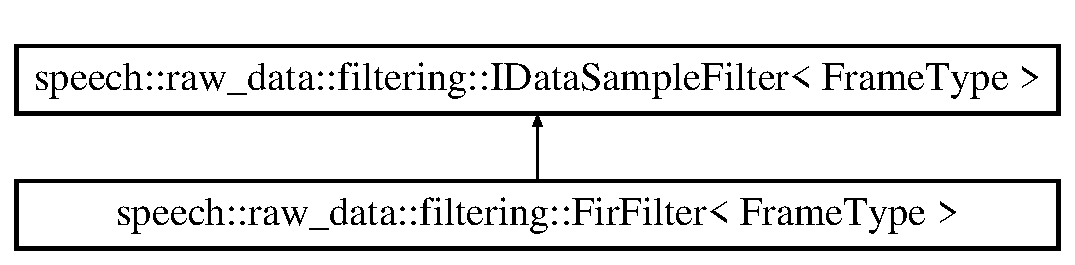
\includegraphics[height=2.000000cm]{classspeech_1_1raw__data_1_1filtering_1_1FirFilter}
\end{center}
\end{figure}
\subsection*{Public Member Functions}
\begin{DoxyCompactItemize}
\item 
\hypertarget{classspeech_1_1raw__data_1_1filtering_1_1FirFilter_aed8d1d76c20929b4ec3d9c83c04580d4}{{\bfseries Fir\+Filter} (const \hyperlink{structspeech_1_1raw__data_1_1filtering_1_1FirFilterData}{Fir\+Filter\+Data} ffd)}\label{classspeech_1_1raw__data_1_1filtering_1_1FirFilter_aed8d1d76c20929b4ec3d9c83c04580d4}

\item 
\hypertarget{classspeech_1_1raw__data_1_1filtering_1_1FirFilter_a96b75db3b4b43d2387bff187d2e2e36f}{virtual \hyperlink{classspeech_1_1raw__data_1_1DataSample}{Data\+Sample}$<$ Frame\+Type $>$ {\bfseries filter} (const \hyperlink{classspeech_1_1raw__data_1_1DataSample}{Data\+Sample}$<$ Frame\+Type $>$ \&sample)}\label{classspeech_1_1raw__data_1_1filtering_1_1FirFilter_a96b75db3b4b43d2387bff187d2e2e36f}

\end{DoxyCompactItemize}


The documentation for this class was generated from the following files\+:\begin{DoxyCompactItemize}
\item 
/home/kacper/\+Projects/speech-\/recognition/src/speech/raw\+\_\+data/filtering/Fir\+Filter.\+h\item 
/home/kacper/\+Projects/speech-\/recognition/src/speech/raw\+\_\+data/filtering/Fir\+Filter.\+cpp\end{DoxyCompactItemize}

\hypertarget{classspeech_1_1raw__data_1_1filtering_1_1FirFilterBank}{\section{speech\+:\+:raw\+\_\+data\+:\+:filtering\+:\+:Fir\+Filter\+Bank Class Reference}
\label{classspeech_1_1raw__data_1_1filtering_1_1FirFilterBank}\index{speech\+::raw\+\_\+data\+::filtering\+::\+Fir\+Filter\+Bank@{speech\+::raw\+\_\+data\+::filtering\+::\+Fir\+Filter\+Bank}}
}
\subsection*{Static Public Attributes}
\begin{DoxyCompactItemize}
\item 
static const \hyperlink{structspeech_1_1raw__data_1_1filtering_1_1FirFilterData}{Fir\+Filter\+Data} \hyperlink{classspeech_1_1raw__data_1_1filtering_1_1FirFilterBank_aa67005c1ebcf970f2826a2d9ee426f1d}{L\+O\+W\+P\+A\+S\+S\+\_\+44100\+\_\+8000\+\_\+5\+D\+B\+\_\+80\+D\+B}
\item 
static const \hyperlink{structspeech_1_1raw__data_1_1filtering_1_1FirFilterData}{Fir\+Filter\+Data} \hyperlink{classspeech_1_1raw__data_1_1filtering_1_1FirFilterBank_a4bd8bcb62eeeb42a4c0fbcf745211af5}{L\+O\+W\+P\+A\+S\+S\+\_\+44100\+\_\+8000\+\_\+3\+D\+B\+\_\+80\+D\+B}
\item 
static const \hyperlink{structspeech_1_1raw__data_1_1filtering_1_1FirFilterData}{Fir\+Filter\+Data} \hyperlink{classspeech_1_1raw__data_1_1filtering_1_1FirFilterBank_a83f13453e59bd6a8d00ba0a8ce9e67f6}{L\+O\+W\+P\+A\+S\+S\+\_\+44100\+\_\+1000\+\_\+3\+D\+B\+\_\+80\+D\+B}
\item 
static const \hyperlink{structspeech_1_1raw__data_1_1filtering_1_1FirFilterData}{Fir\+Filter\+Data} \hyperlink{classspeech_1_1raw__data_1_1filtering_1_1FirFilterBank_a3fe4a0224ec1af6c10d6cb760dd1d336}{H\+I\+G\+H\+P\+A\+S\+S\+\_\+44100\+\_\+3000\+\_\+3\+D\+B\+\_\+80\+D\+B}
\item 
static const \hyperlink{structspeech_1_1raw__data_1_1filtering_1_1FirFilterData}{Fir\+Filter\+Data} \hyperlink{classspeech_1_1raw__data_1_1filtering_1_1FirFilterBank_ab62552f4111d615c675582de6378e462}{H\+I\+G\+H\+P\+A\+S\+S\+\_\+44100\+\_\+8000\+\_\+3\+D\+B\+\_\+80\+D\+B}
\item 
static const \hyperlink{structspeech_1_1raw__data_1_1filtering_1_1FirFilterData}{Fir\+Filter\+Data} \hyperlink{classspeech_1_1raw__data_1_1filtering_1_1FirFilterBank_a28029922c12b58351adda2556609499d}{B\+A\+N\+D\+P\+A\+S\+S\+\_\+44100\+\_\+2000\+\_\+5000\+\_\+5\+D\+B\+\_\+60\+D\+B}
\item 
static const \hyperlink{structspeech_1_1raw__data_1_1filtering_1_1FirFilterData}{Fir\+Filter\+Data} \hyperlink{classspeech_1_1raw__data_1_1filtering_1_1FirFilterBank_aaecaed690bc2ca0ec02ae8dd29491d15}{B\+A\+N\+D\+S\+T\+O\+P\+\_\+44100\+\_\+2000\+\_\+5000\+\_\+3\+D\+B\+\_\+60\+D\+B}
\end{DoxyCompactItemize}


\subsection{Member Data Documentation}
\hypertarget{classspeech_1_1raw__data_1_1filtering_1_1FirFilterBank_a28029922c12b58351adda2556609499d}{\index{speech\+::raw\+\_\+data\+::filtering\+::\+Fir\+Filter\+Bank@{speech\+::raw\+\_\+data\+::filtering\+::\+Fir\+Filter\+Bank}!B\+A\+N\+D\+P\+A\+S\+S\+\_\+44100\+\_\+2000\+\_\+5000\+\_\+5\+D\+B\+\_\+60\+D\+B@{B\+A\+N\+D\+P\+A\+S\+S\+\_\+44100\+\_\+2000\+\_\+5000\+\_\+5\+D\+B\+\_\+60\+D\+B}}
\index{B\+A\+N\+D\+P\+A\+S\+S\+\_\+44100\+\_\+2000\+\_\+5000\+\_\+5\+D\+B\+\_\+60\+D\+B@{B\+A\+N\+D\+P\+A\+S\+S\+\_\+44100\+\_\+2000\+\_\+5000\+\_\+5\+D\+B\+\_\+60\+D\+B}!speech\+::raw\+\_\+data\+::filtering\+::\+Fir\+Filter\+Bank@{speech\+::raw\+\_\+data\+::filtering\+::\+Fir\+Filter\+Bank}}
\subsubsection[{B\+A\+N\+D\+P\+A\+S\+S\+\_\+44100\+\_\+2000\+\_\+5000\+\_\+5\+D\+B\+\_\+60\+D\+B}]{\setlength{\rightskip}{0pt plus 5cm}const {\bf speech\+::raw\+\_\+data\+::filtering\+::\+Fir\+Filter\+Data} speech\+::raw\+\_\+data\+::filtering\+::\+Fir\+Filter\+Bank\+::\+B\+A\+N\+D\+P\+A\+S\+S\+\_\+44100\+\_\+2000\+\_\+5000\+\_\+5\+D\+B\+\_\+60\+D\+B\hspace{0.3cm}{\ttfamily [static]}}}\label{classspeech_1_1raw__data_1_1filtering_1_1FirFilterBank_a28029922c12b58351adda2556609499d}
{\bfseries Initial value\+:}
\begin{DoxyCode}
= \{
        79, (\textcolor{keywordtype}{double}[]) \{0.00112, 0.001683, 0.002146, 0.001926, 0.0008857, -0.0006888, -0.002125, -0.002706,
       -0.002135,
                        -0.0009, -0.0002116, -0.001451, -0.005263, -0.01081, -0.01565, -0.01652, -0.01091, 
      0.001361,
                        0.01739, 0.03182, 0.03892, 0.03529, 0.02183, 0.003877, -0.01088, -0.01605, -0.01004
      , 0.002522,
                        0.01227, 0.009435, -0.0109, -0.04519, -0.08133, -0.1029, -0.0958, -0.05536, 0.01066
      , 0.08352,
                        0.14, 0.1613, 0.14, 0.08352, 0.01066, -0.05536, -0.0958, -0.1029, -0.08133, -0.0451
      9, -0.0109,
                        0.009435, 0.01227, 0.002522, -0.01004, -0.01605, -0.01088, 0.003877, 0.02183, 0.035
      29, 0.03892,
                        0.03182, 0.01739, 0.001361, -0.01091, -0.01652, -0.01565, -0.01081, -0.005263, -0.0
      01451,
                        -0.0002116, -0.0009, -0.002135, -0.002706, -0.002125, -0.0006888, 0.0008857, 0.0019
      26, 0.002146,
                        0.001683, 0.00112\}\}
\end{DoxyCode}
\{             gain\+: 0, // stopband             atten\+: -\/60d\+B,             start\+: 0\+Hz,             stop\+: 1000\+Hz         \},                          \{             gain\+: 1, // passband             ripple\+: 5d\+B,             start\+: 2000\+Hz,             stop\+: 5000\+Hz         \},

        \{             gain\+: 0, // stopband             atten\+: -\/60d\+B,             start\+: 6000\+Hz,             stop\+: 22000\+Hz         \} \hypertarget{classspeech_1_1raw__data_1_1filtering_1_1FirFilterBank_aaecaed690bc2ca0ec02ae8dd29491d15}{\index{speech\+::raw\+\_\+data\+::filtering\+::\+Fir\+Filter\+Bank@{speech\+::raw\+\_\+data\+::filtering\+::\+Fir\+Filter\+Bank}!B\+A\+N\+D\+S\+T\+O\+P\+\_\+44100\+\_\+2000\+\_\+5000\+\_\+3\+D\+B\+\_\+60\+D\+B@{B\+A\+N\+D\+S\+T\+O\+P\+\_\+44100\+\_\+2000\+\_\+5000\+\_\+3\+D\+B\+\_\+60\+D\+B}}
\index{B\+A\+N\+D\+S\+T\+O\+P\+\_\+44100\+\_\+2000\+\_\+5000\+\_\+3\+D\+B\+\_\+60\+D\+B@{B\+A\+N\+D\+S\+T\+O\+P\+\_\+44100\+\_\+2000\+\_\+5000\+\_\+3\+D\+B\+\_\+60\+D\+B}!speech\+::raw\+\_\+data\+::filtering\+::\+Fir\+Filter\+Bank@{speech\+::raw\+\_\+data\+::filtering\+::\+Fir\+Filter\+Bank}}
\subsubsection[{B\+A\+N\+D\+S\+T\+O\+P\+\_\+44100\+\_\+2000\+\_\+5000\+\_\+3\+D\+B\+\_\+60\+D\+B}]{\setlength{\rightskip}{0pt plus 5cm}const {\bf speech\+::raw\+\_\+data\+::filtering\+::\+Fir\+Filter\+Data} speech\+::raw\+\_\+data\+::filtering\+::\+Fir\+Filter\+Bank\+::\+B\+A\+N\+D\+S\+T\+O\+P\+\_\+44100\+\_\+2000\+\_\+5000\+\_\+3\+D\+B\+\_\+60\+D\+B\hspace{0.3cm}{\ttfamily [static]}}}\label{classspeech_1_1raw__data_1_1filtering_1_1FirFilterBank_aaecaed690bc2ca0ec02ae8dd29491d15}
{\bfseries Initial value\+:}
\begin{DoxyCode}
= \{
        85,
        (\textcolor{keywordtype}{double}[]) \{0.01649, -0.03374, 0.01985, 0.008045, -0.01096, -0.01039, 0.002568, 0.008872, 0.001908,
       -0.01077,
                    -0.01665, -0.01195, -0.001938, 0.003685, 0.0004378, -0.009659, -0.01918, -0.02241, -0.0
      1725,
                    -0.007531, 0.001239, 0.003502, -0.001487, -0.01078, -0.01743, -0.0159, -0.003822, 0.014
      12, 0.02987,
                    0.03465, 0.02646, 0.01058, -0.0003171, 0.005068, 0.03104, 0.06834, 0.09854, 0.1001, 0.0
      6147,
                    -0.01279, -0.1005, -0.1713, 0.8019, -0.1713, -0.1005, -0.01279, 0.06147, 0.1001, 0.0985
      4, 0.06834,
                    0.03104, 0.005068, -0.0003171, 0.01058, 0.02646, 0.03465, 0.02987, 0.01412, -0.003822, 
      -0.0159,
                    -0.01743, -0.01078, -0.001487, 0.003502, 0.001239, -0.007531, -0.01725, -0.02241, -0.01
      918,
                    -0.009659, 0.0004378, 0.003685, -0.001938, -0.01195, -0.01665, -0.01077, 0.001908, 0.00
      8872,
                    0.002568, -0.01039, -0.01096, 0.008045, 0.01985, -0.03374, 0.01649\}\}
\end{DoxyCode}
\{             gain\+: 1, // passband             ripple\+: 3d\+B,             start\+: 0\+Hz,             stop\+: 1000\+Hz         \},                          \{             gain\+: 0, // stopband             atten\+: -\/60d\+B,             start\+: 2000\+Hz,             stop\+: 5000\+Hz         \},

        \{             gain\+: 1, // passband             ripple\+: 3d\+B,             start\+: 6000\+Hz,             stop\+: 22000\+Hz         \} \hypertarget{classspeech_1_1raw__data_1_1filtering_1_1FirFilterBank_a3fe4a0224ec1af6c10d6cb760dd1d336}{\index{speech\+::raw\+\_\+data\+::filtering\+::\+Fir\+Filter\+Bank@{speech\+::raw\+\_\+data\+::filtering\+::\+Fir\+Filter\+Bank}!H\+I\+G\+H\+P\+A\+S\+S\+\_\+44100\+\_\+3000\+\_\+3\+D\+B\+\_\+80\+D\+B@{H\+I\+G\+H\+P\+A\+S\+S\+\_\+44100\+\_\+3000\+\_\+3\+D\+B\+\_\+80\+D\+B}}
\index{H\+I\+G\+H\+P\+A\+S\+S\+\_\+44100\+\_\+3000\+\_\+3\+D\+B\+\_\+80\+D\+B@{H\+I\+G\+H\+P\+A\+S\+S\+\_\+44100\+\_\+3000\+\_\+3\+D\+B\+\_\+80\+D\+B}!speech\+::raw\+\_\+data\+::filtering\+::\+Fir\+Filter\+Bank@{speech\+::raw\+\_\+data\+::filtering\+::\+Fir\+Filter\+Bank}}
\subsubsection[{H\+I\+G\+H\+P\+A\+S\+S\+\_\+44100\+\_\+3000\+\_\+3\+D\+B\+\_\+80\+D\+B}]{\setlength{\rightskip}{0pt plus 5cm}const {\bf speech\+::raw\+\_\+data\+::filtering\+::\+Fir\+Filter\+Data} speech\+::raw\+\_\+data\+::filtering\+::\+Fir\+Filter\+Bank\+::\+H\+I\+G\+H\+P\+A\+S\+S\+\_\+44100\+\_\+3000\+\_\+3\+D\+B\+\_\+80\+D\+B\hspace{0.3cm}{\ttfamily [static]}}}\label{classspeech_1_1raw__data_1_1filtering_1_1FirFilterBank_a3fe4a0224ec1af6c10d6cb760dd1d336}
{\bfseries Initial value\+:}
\begin{DoxyCode}
= \{
        95,
        (\textcolor{keywordtype}{double}[]) \{0.03013, -0.04622, -0.009993, 0.007307, 0.01332, 0.0124, 0.008554, 0.003378, -0.001202,
       -0.005073,
                    -0.007254, -0.008244, -0.007528, -0.005905, -0.003069, -0.00002909, 0.003394, 0.006125,
       0.008363,
                    0.009131, 0.00883, 0.00679, 0.003804, -0.0004484, -0.004753, -0.009113, -0.01218, -0.01
      398,
                    -0.01338, -0.01091, -0.005902, 0.0004914, 0.008097, 0.0154, 0.02157, 0.0251, 0.0254, 0.
      02112,
                    0.01256, -0.0007717, -0.01771, -0.03764, -0.05847, -0.07914, -0.09733, -0.1119, -0.121,
       0.8757,
                    -0.121, -0.1119, -0.09733, -0.07914, -0.05847, -0.03764, -0.01771, -0.0007717, 0.01256,
       0.02112,
                    0.0254, 0.0251, 0.02157, 0.0154, 0.008097, 0.0004914, -0.005902, -0.01091, -0.01338, -0
      .01398,
                    -0.01218, -0.009113, -0.004753, -0.0004484, 0.003804, 0.00679, 0.00883, 0.009131, 0.008
      363,
                    0.006125, 0.003394, -0.00002909, -0.003069, -0.005905, -0.007528, -0.008244, -0.007254,
       -0.005073,
                    -0.001202, 0.003378, 0.008554, 0.0124, 0.01332, 0.007307, -0.009993, -0.04622, 0.03013\}
      \}
\end{DoxyCode}
\{             gain\+: 0, // stopband             atten\+: -\/80d\+B,             start\+: 0\+Hz,             stop\+: 2000\+Hz         \},                          \{             gain\+: 1, // passband             ripple\+: 3d\+B,             start\+: 3000\+Hz,             stop\+: 22000\+Hz         \} \hypertarget{classspeech_1_1raw__data_1_1filtering_1_1FirFilterBank_ab62552f4111d615c675582de6378e462}{\index{speech\+::raw\+\_\+data\+::filtering\+::\+Fir\+Filter\+Bank@{speech\+::raw\+\_\+data\+::filtering\+::\+Fir\+Filter\+Bank}!H\+I\+G\+H\+P\+A\+S\+S\+\_\+44100\+\_\+8000\+\_\+3\+D\+B\+\_\+80\+D\+B@{H\+I\+G\+H\+P\+A\+S\+S\+\_\+44100\+\_\+8000\+\_\+3\+D\+B\+\_\+80\+D\+B}}
\index{H\+I\+G\+H\+P\+A\+S\+S\+\_\+44100\+\_\+8000\+\_\+3\+D\+B\+\_\+80\+D\+B@{H\+I\+G\+H\+P\+A\+S\+S\+\_\+44100\+\_\+8000\+\_\+3\+D\+B\+\_\+80\+D\+B}!speech\+::raw\+\_\+data\+::filtering\+::\+Fir\+Filter\+Bank@{speech\+::raw\+\_\+data\+::filtering\+::\+Fir\+Filter\+Bank}}
\subsubsection[{H\+I\+G\+H\+P\+A\+S\+S\+\_\+44100\+\_\+8000\+\_\+3\+D\+B\+\_\+80\+D\+B}]{\setlength{\rightskip}{0pt plus 5cm}const {\bf speech\+::raw\+\_\+data\+::filtering\+::\+Fir\+Filter\+Data} speech\+::raw\+\_\+data\+::filtering\+::\+Fir\+Filter\+Bank\+::\+H\+I\+G\+H\+P\+A\+S\+S\+\_\+44100\+\_\+8000\+\_\+3\+D\+B\+\_\+80\+D\+B\hspace{0.3cm}{\ttfamily [static]}}}\label{classspeech_1_1raw__data_1_1filtering_1_1FirFilterBank_ab62552f4111d615c675582de6378e462}
{\bfseries Initial value\+:}
\begin{DoxyCode}
= \{
        107,
        (\textcolor{keywordtype}{double}[]) \{-0.001545, 0.001346, 0.01087, -0.02704, 0.01886, 0.00598, -0.006693, -0.008108, 0.00153
      , 0.007125,
                    0.003618, -0.003826, -0.006074, -0.001445, 0.004851, 0.005398, 0.00005067, -0.005703, -
      0.005066,
                    0.001258, 0.006704, 0.004731, -0.002696, -0.007859, -0.004283, 0.004471, 0.009146, 0.00
      3506,
                    -0.006668, -0.01044, -0.002316, 0.009358, 0.01176, 0.0005111, -0.0127, -0.01303, 0.0021
      56, 0.01693,
                    0.01419, -0.006103, -0.02252, -0.0152, 0.01218, 0.03057, 0.01603, -0.02253, -0.04408, -
      0.01662,
                    0.04435, 0.07527, 0.01701, -0.1284, -0.2836, 0.6495, -0.2836, -0.1284, 0.01701, 0.07527
      , 0.04435,
                    -0.01662, -0.04408, -0.02253, 0.01603, 0.03057, 0.01218, -0.0152, -0.02252, -0.006103, 
      0.01419,
                    0.01693, 0.002156, -0.01303, -0.0127, 0.0005111, 0.01176, 0.009358, -0.002316, -0.01044
      , -0.006668,
                    0.003506, 0.009146, 0.004471, -0.004283, -0.007859, -0.002696, 0.004731, 0.006704, 0.00
      1258,
                    -0.005066, -0.005703, 0.00005067, 0.005398, 0.004851, -0.001445, -0.006074, -0.003826, 
      0.003618,
                    0.007125, 0.00153, -0.008108, -0.006693, 0.00598, 0.01886, -0.02704, 0.01087, 0.001346,
       -0.001545\}\}
\end{DoxyCode}
\{             gain\+: 0, // stopband             atten\+: -\/80d\+B,             start\+: 0\+Hz,             stop\+: 7000\+Hz         \},                          \{             gain\+: 1, // passband             ripple\+: 3d\+B,             start\+: 8000\+Hz,             stop\+: 22000\+Hz         \} \hypertarget{classspeech_1_1raw__data_1_1filtering_1_1FirFilterBank_a83f13453e59bd6a8d00ba0a8ce9e67f6}{\index{speech\+::raw\+\_\+data\+::filtering\+::\+Fir\+Filter\+Bank@{speech\+::raw\+\_\+data\+::filtering\+::\+Fir\+Filter\+Bank}!L\+O\+W\+P\+A\+S\+S\+\_\+44100\+\_\+1000\+\_\+3\+D\+B\+\_\+80\+D\+B@{L\+O\+W\+P\+A\+S\+S\+\_\+44100\+\_\+1000\+\_\+3\+D\+B\+\_\+80\+D\+B}}
\index{L\+O\+W\+P\+A\+S\+S\+\_\+44100\+\_\+1000\+\_\+3\+D\+B\+\_\+80\+D\+B@{L\+O\+W\+P\+A\+S\+S\+\_\+44100\+\_\+1000\+\_\+3\+D\+B\+\_\+80\+D\+B}!speech\+::raw\+\_\+data\+::filtering\+::\+Fir\+Filter\+Bank@{speech\+::raw\+\_\+data\+::filtering\+::\+Fir\+Filter\+Bank}}
\subsubsection[{L\+O\+W\+P\+A\+S\+S\+\_\+44100\+\_\+1000\+\_\+3\+D\+B\+\_\+80\+D\+B}]{\setlength{\rightskip}{0pt plus 5cm}const {\bf speech\+::raw\+\_\+data\+::filtering\+::\+Fir\+Filter\+Data} speech\+::raw\+\_\+data\+::filtering\+::\+Fir\+Filter\+Bank\+::\+L\+O\+W\+P\+A\+S\+S\+\_\+44100\+\_\+1000\+\_\+3\+D\+B\+\_\+80\+D\+B\hspace{0.3cm}{\ttfamily [static]}}}\label{classspeech_1_1raw__data_1_1filtering_1_1FirFilterBank_a83f13453e59bd6a8d00ba0a8ce9e67f6}
{\bfseries Initial value\+:}
\begin{DoxyCode}
= \{
        59, (\textcolor{keywordtype}{double}[]) \{-0.0001071, -0.0001666, -0.0002774, -0.0004146, -0.000568, -0.0007174, -0.0008323, 
      -0.0008696,
                        -0.0007747, -0.0004816, 0.0000837, 0.001, 0.002347, 0.004196, 0.006608, 0.009621, 0
      .01325,
                        0.01748, 0.02225, 0.02748, 0.03304, 0.03879, 0.04453, 0.05007, 0.0552, 0.05973, 0.0
      6347,
                        0.06626,
                        0.06798, 0.06857, 0.06798, 0.06626, 0.06347, 0.05973, 0.0552, 0.05007, 0.04453, 0.0
      3879,
                        0.03304,
                        0.02748, 0.02225, 0.01748, 0.01325, 0.009621, 0.006608, 0.004196, 0.002347, 0.001, 
      0.0000837,
                        -0.0004816,
                        -0.0007747, -0.0008696, -0.0008323, -0.0007174, -0.000568, -0.0004146, -0.0002774, 
      -0.0001666,
                        -0.0001071\}\}
\end{DoxyCode}
\{             gain\+: 1, // passband             ripple\+: 5d\+B,             start\+: 0\+Hz,             stop\+: 1000\+Hz         \},                          \{             gain\+: 0, // stopband             atten\+: -\/80d\+B,             start\+: 3000\+Hz,             stop\+: 22000\+Hz         \} \hypertarget{classspeech_1_1raw__data_1_1filtering_1_1FirFilterBank_a4bd8bcb62eeeb42a4c0fbcf745211af5}{\index{speech\+::raw\+\_\+data\+::filtering\+::\+Fir\+Filter\+Bank@{speech\+::raw\+\_\+data\+::filtering\+::\+Fir\+Filter\+Bank}!L\+O\+W\+P\+A\+S\+S\+\_\+44100\+\_\+8000\+\_\+3\+D\+B\+\_\+80\+D\+B@{L\+O\+W\+P\+A\+S\+S\+\_\+44100\+\_\+8000\+\_\+3\+D\+B\+\_\+80\+D\+B}}
\index{L\+O\+W\+P\+A\+S\+S\+\_\+44100\+\_\+8000\+\_\+3\+D\+B\+\_\+80\+D\+B@{L\+O\+W\+P\+A\+S\+S\+\_\+44100\+\_\+8000\+\_\+3\+D\+B\+\_\+80\+D\+B}!speech\+::raw\+\_\+data\+::filtering\+::\+Fir\+Filter\+Bank@{speech\+::raw\+\_\+data\+::filtering\+::\+Fir\+Filter\+Bank}}
\subsubsection[{L\+O\+W\+P\+A\+S\+S\+\_\+44100\+\_\+8000\+\_\+3\+D\+B\+\_\+80\+D\+B}]{\setlength{\rightskip}{0pt plus 5cm}const {\bf speech\+::raw\+\_\+data\+::filtering\+::\+Fir\+Filter\+Data} speech\+::raw\+\_\+data\+::filtering\+::\+Fir\+Filter\+Bank\+::\+L\+O\+W\+P\+A\+S\+S\+\_\+44100\+\_\+8000\+\_\+3\+D\+B\+\_\+80\+D\+B\hspace{0.3cm}{\ttfamily [static]}}}\label{classspeech_1_1raw__data_1_1filtering_1_1FirFilterBank_a4bd8bcb62eeeb42a4c0fbcf745211af5}
{\bfseries Initial value\+:}
\begin{DoxyCode}
= \{
        53,
        (\textcolor{keywordtype}{double}[]) \{0.0008437, 0.003316, 0.006353, 0.00584, -0.002333, -0.01613, -0.02543, -0.02021, -0.002
      916, 0.01017,
                    0.00508, -0.01195, -0.01846, -0.00242, 0.01902, 0.01683, -0.01158, -0.03159, -0.01075, 
      0.03341,
                    0.04246, -0.0125, -0.07682, -0.0508, 0.103, 0.298, 0.3871, 0.298, 0.103, -0.0508, -0.07
      682, -0.0125,
                    0.04246, 0.03341, -0.01075, -0.03159, -0.01158, 0.01683, 0.01902, -0.00242, -0.01846, -
      0.01195,
                    0.00508, 0.01017, -0.002916, -0.02021, -0.02543, -0.01613, -0.002333, 0.00584, 0.006353
      , 0.003316,
                    0.0008437\}\}
\end{DoxyCode}
\{             gain\+: 1, // passband             ripple\+: 3d\+B,             start\+: 0\+Hz,             stop\+: 8000\+Hz         \},                          \{             gain\+: 0, // stopband             atten\+: -\/80d\+B,             start\+: 10000\+Hz,             stop\+: 22000\+Hz         \} \hypertarget{classspeech_1_1raw__data_1_1filtering_1_1FirFilterBank_aa67005c1ebcf970f2826a2d9ee426f1d}{\index{speech\+::raw\+\_\+data\+::filtering\+::\+Fir\+Filter\+Bank@{speech\+::raw\+\_\+data\+::filtering\+::\+Fir\+Filter\+Bank}!L\+O\+W\+P\+A\+S\+S\+\_\+44100\+\_\+8000\+\_\+5\+D\+B\+\_\+80\+D\+B@{L\+O\+W\+P\+A\+S\+S\+\_\+44100\+\_\+8000\+\_\+5\+D\+B\+\_\+80\+D\+B}}
\index{L\+O\+W\+P\+A\+S\+S\+\_\+44100\+\_\+8000\+\_\+5\+D\+B\+\_\+80\+D\+B@{L\+O\+W\+P\+A\+S\+S\+\_\+44100\+\_\+8000\+\_\+5\+D\+B\+\_\+80\+D\+B}!speech\+::raw\+\_\+data\+::filtering\+::\+Fir\+Filter\+Bank@{speech\+::raw\+\_\+data\+::filtering\+::\+Fir\+Filter\+Bank}}
\subsubsection[{L\+O\+W\+P\+A\+S\+S\+\_\+44100\+\_\+8000\+\_\+5\+D\+B\+\_\+80\+D\+B}]{\setlength{\rightskip}{0pt plus 5cm}const {\bf speech\+::raw\+\_\+data\+::filtering\+::\+Fir\+Filter\+Data} speech\+::raw\+\_\+data\+::filtering\+::\+Fir\+Filter\+Bank\+::\+L\+O\+W\+P\+A\+S\+S\+\_\+44100\+\_\+8000\+\_\+5\+D\+B\+\_\+80\+D\+B\hspace{0.3cm}{\ttfamily [static]}}}\label{classspeech_1_1raw__data_1_1filtering_1_1FirFilterBank_aa67005c1ebcf970f2826a2d9ee426f1d}
{\bfseries Initial value\+:}
\begin{DoxyCode}
= \{
        89, (\textcolor{keywordtype}{double}[]) \{0.000301, 0.0003093, -0.00181, -0.008632, -0.0207, -0.03364, -0.03894, -0.02982,
                        -0.008534, 0.01248, 0.01923, 0.00838, -0.008548, -0.0151, -0.005578, 0.009184,
                        0.01307, 0.002017, -0.01125, -0.01128, 0.002275, 0.01357, 0.00867, -0.007391,
                        -0.01539, -0.004534, 0.01324, 0.01595, -0.001701, -0.01952, -0.01434, 0.01061,
                        0.02579, 0.009302, -0.02316, -0.03144, 0.001654, 0.04216, 0.03602, -0.02573,
                        -0.07925, -0.03897, 0.1136, 0.2934, 0.3733, 0.2934, 0.1136, -0.03897, -0.07925,
                        -0.02573, 0.03602, 0.04216, 0.001654, -0.03144, -0.02316, 0.009302, 0.02579, 0.0106
      1,
                        -0.01434, -0.01952, -0.001701, 0.01595, 0.01324, -0.004534, -0.01539, -0.007391,
                        0.00867, 0.01357, 0.002275, -0.01128, -0.01125, 0.002017, 0.01307, 0.009184,
                        -0.005578, -0.0151, -0.008548, 0.00838, 0.01923, 0.01248, -0.008534, -0.02982,
                        -0.03894, -0.03364, -0.0207, -0.008632, -0.00181, 0.0003093, 0.000301\}\}
\end{DoxyCode}
\{             gain\+: 1, // passband             ripple\+: 5d\+B,             start\+: 0\+Hz,             stop\+: 8000\+Hz         \},                          \{             gain\+: 0, // stopband             atten\+: -\/80d\+B,             start\+: 9000\+Hz,             stop\+: 22000\+Hz         \} 

The documentation for this class was generated from the following files\+:\begin{DoxyCompactItemize}
\item 
/home/kacper/\+Projects/speech-\/recognition/src/speech/raw\+\_\+data/filtering/Fir\+Filter\+Bank.\+h\item 
/home/kacper/\+Projects/speech-\/recognition/src/speech/raw\+\_\+data/filtering/Fir\+Filter\+Bank.\+cpp\end{DoxyCompactItemize}

\hypertarget{structspeech_1_1raw__data_1_1filtering_1_1FirFilterData}{\section{speech\+:\+:raw\+\_\+data\+:\+:filtering\+:\+:Fir\+Filter\+Data Struct Reference}
\label{structspeech_1_1raw__data_1_1filtering_1_1FirFilterData}\index{speech\+::raw\+\_\+data\+::filtering\+::\+Fir\+Filter\+Data@{speech\+::raw\+\_\+data\+::filtering\+::\+Fir\+Filter\+Data}}
}
\subsection*{Public Attributes}
\begin{DoxyCompactItemize}
\item 
\hypertarget{structspeech_1_1raw__data_1_1filtering_1_1FirFilterData_ac54e8602d9ee04b36c382a6542d3a0c1}{int {\bfseries num\+Taps}}\label{structspeech_1_1raw__data_1_1filtering_1_1FirFilterData_ac54e8602d9ee04b36c382a6542d3a0c1}

\item 
\hypertarget{structspeech_1_1raw__data_1_1filtering_1_1FirFilterData_a91b76611e548be176a437e751036f23f}{double $\ast$ {\bfseries taps}}\label{structspeech_1_1raw__data_1_1filtering_1_1FirFilterData_a91b76611e548be176a437e751036f23f}

\end{DoxyCompactItemize}


The documentation for this struct was generated from the following file\+:\begin{DoxyCompactItemize}
\item 
/home/kacper/\+Projects/speech-\/recognition/src/speech/raw\+\_\+data/filtering/Fir\+Filter\+Bank.\+h\end{DoxyCompactItemize}

\hypertarget{classspeech_1_1vectorizer_1_1FormantVectorizer}{\section{speech\+:\+:vectorizer\+:\+:Formant\+Vectorizer$<$ Frame\+Type $>$ Class Template Reference}
\label{classspeech_1_1vectorizer_1_1FormantVectorizer}\index{speech\+::vectorizer\+::\+Formant\+Vectorizer$<$ Frame\+Type $>$@{speech\+::vectorizer\+::\+Formant\+Vectorizer$<$ Frame\+Type $>$}}
}


{\ttfamily \#include $<$Formant\+Vectorizer.\+h$>$}

Inheritance diagram for speech\+:\+:vectorizer\+:\+:Formant\+Vectorizer$<$ Frame\+Type $>$\+:\begin{figure}[H]
\begin{center}
\leavevmode
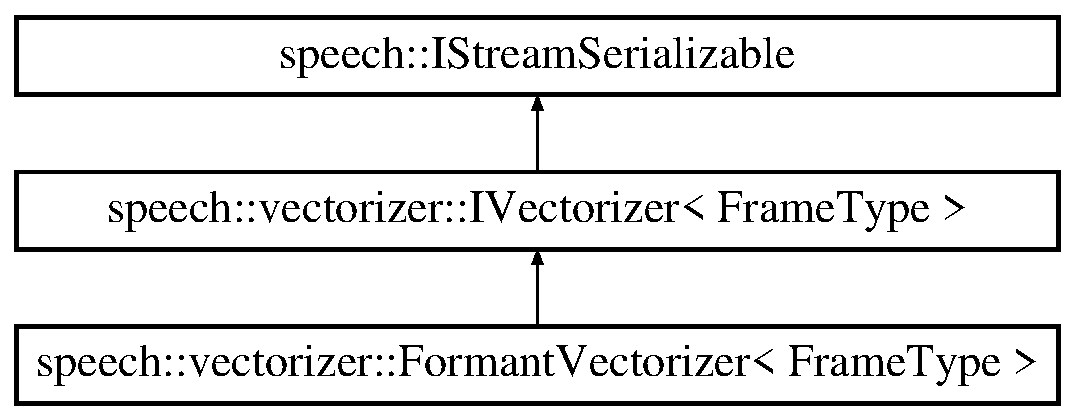
\includegraphics[height=3.000000cm]{classspeech_1_1vectorizer_1_1FormantVectorizer}
\end{center}
\end{figure}
\subsection*{Public Member Functions}
\begin{DoxyCompactItemize}
\item 
\hypertarget{classspeech_1_1vectorizer_1_1FormantVectorizer_abef2f775e105e837befb8e0f3ed24086}{{\bfseries Formant\+Vectorizer} (std\+::istream \&in)}\label{classspeech_1_1vectorizer_1_1FormantVectorizer_abef2f775e105e837befb8e0f3ed24086}

\item 
virtual std\+::valarray$<$ double $>$ \hyperlink{classspeech_1_1vectorizer_1_1FormantVectorizer_a80e578bcd5f23d4b9237589669e20a1a}{vectorize} (\hyperlink{classspeech_1_1raw__data_1_1FrequencySample}{Frequency\+Sample}$<$ Frame\+Type $>$ \&sample)
\item 
virtual void \hyperlink{classspeech_1_1vectorizer_1_1FormantVectorizer_a8eed42b42272eb0d77a49213a5a36f73}{serialize} (std\+::ostream \&out) const 
\item 
virtual int \hyperlink{classspeech_1_1vectorizer_1_1FormantVectorizer_a50b6e8aeace5dab5f7365b57477b7333}{get\+Vector\+Size} () const 
\end{DoxyCompactItemize}
\subsection*{Static Public Attributes}
\begin{DoxyCompactItemize}
\item 
\hypertarget{classspeech_1_1vectorizer_1_1FormantVectorizer_a4876130f4b7695e317afe455e1baafc6}{static const uint32\+\_\+t {\bfseries T\+Y\+P\+E\+\_\+\+I\+D\+E\+N\+T\+I\+F\+I\+E\+R} = 0x00100002}\label{classspeech_1_1vectorizer_1_1FormantVectorizer_a4876130f4b7695e317afe455e1baafc6}

\end{DoxyCompactItemize}
\subsection*{Additional Inherited Members}


\subsection{Detailed Description}
\subsubsection*{template$<$typename Frame\+Type$>$class speech\+::vectorizer\+::\+Formant\+Vectorizer$<$ Frame\+Type $>$}

Vectorizer getting formants from samples and converting them into the vector space. 

\subsection{Member Function Documentation}
\hypertarget{classspeech_1_1vectorizer_1_1FormantVectorizer_a50b6e8aeace5dab5f7365b57477b7333}{\index{speech\+::vectorizer\+::\+Formant\+Vectorizer@{speech\+::vectorizer\+::\+Formant\+Vectorizer}!get\+Vector\+Size@{get\+Vector\+Size}}
\index{get\+Vector\+Size@{get\+Vector\+Size}!speech\+::vectorizer\+::\+Formant\+Vectorizer@{speech\+::vectorizer\+::\+Formant\+Vectorizer}}
\subsubsection[{get\+Vector\+Size}]{\setlength{\rightskip}{0pt plus 5cm}template$<$typename Frame\+Type $>$ int {\bf speech\+::vectorizer\+::\+Formant\+Vectorizer}$<$ Frame\+Type $>$\+::get\+Vector\+Size (
\begin{DoxyParamCaption}
{}
\end{DoxyParamCaption}
) const\hspace{0.3cm}{\ttfamily [virtual]}}}\label{classspeech_1_1vectorizer_1_1FormantVectorizer_a50b6e8aeace5dab5f7365b57477b7333}
Gets the size of the output vector produced by the vectorizer.

\begin{DoxyReturn}{Returns}
size of the produced vector 
\end{DoxyReturn}


Implements \hyperlink{classspeech_1_1vectorizer_1_1IVectorizer_abe20529a1586c072783f42476ad7ab69}{speech\+::vectorizer\+::\+I\+Vectorizer$<$ Frame\+Type $>$}.

\hypertarget{classspeech_1_1vectorizer_1_1FormantVectorizer_a8eed42b42272eb0d77a49213a5a36f73}{\index{speech\+::vectorizer\+::\+Formant\+Vectorizer@{speech\+::vectorizer\+::\+Formant\+Vectorizer}!serialize@{serialize}}
\index{serialize@{serialize}!speech\+::vectorizer\+::\+Formant\+Vectorizer@{speech\+::vectorizer\+::\+Formant\+Vectorizer}}
\subsubsection[{serialize}]{\setlength{\rightskip}{0pt plus 5cm}template$<$typename Frame\+Type $>$ void {\bf speech\+::vectorizer\+::\+Formant\+Vectorizer}$<$ Frame\+Type $>$\+::serialize (
\begin{DoxyParamCaption}
\item[{std\+::ostream \&}]{out}
\end{DoxyParamCaption}
) const\hspace{0.3cm}{\ttfamily [virtual]}}}\label{classspeech_1_1vectorizer_1_1FormantVectorizer_a8eed42b42272eb0d77a49213a5a36f73}
Serializes the vectorizer into given stream. 
\begin{DoxyParams}{Parameters}
{\em out} & output stream \\
\hline
\end{DoxyParams}


Implements \hyperlink{classspeech_1_1vectorizer_1_1IVectorizer_aa8285bbd275c31ae1ce48d294400dea9}{speech\+::vectorizer\+::\+I\+Vectorizer$<$ Frame\+Type $>$}.

\hypertarget{classspeech_1_1vectorizer_1_1FormantVectorizer_a80e578bcd5f23d4b9237589669e20a1a}{\index{speech\+::vectorizer\+::\+Formant\+Vectorizer@{speech\+::vectorizer\+::\+Formant\+Vectorizer}!vectorize@{vectorize}}
\index{vectorize@{vectorize}!speech\+::vectorizer\+::\+Formant\+Vectorizer@{speech\+::vectorizer\+::\+Formant\+Vectorizer}}
\subsubsection[{vectorize}]{\setlength{\rightskip}{0pt plus 5cm}template$<$typename Frame\+Type $>$ std\+::valarray$<$ double $>$ {\bf speech\+::vectorizer\+::\+Formant\+Vectorizer}$<$ Frame\+Type $>$\+::vectorize (
\begin{DoxyParamCaption}
\item[{{\bf Frequency\+Sample}$<$ Frame\+Type $>$ \&}]{sample}
\end{DoxyParamCaption}
)\hspace{0.3cm}{\ttfamily [virtual]}}}\label{classspeech_1_1vectorizer_1_1FormantVectorizer_a80e578bcd5f23d4b9237589669e20a1a}
Projects given sample into feature space. Each vector needs to have exactly same size. 
\begin{DoxyParams}{Parameters}
{\em sample} & single sample to be vectorized\\
\hline
\end{DoxyParams}
\begin{DoxyReturn}{Returns}
the projection of vector in a feature space 
\end{DoxyReturn}


Implements \hyperlink{classspeech_1_1vectorizer_1_1IVectorizer_a00d2ba71ec5c447780ffb0a29bfc9085}{speech\+::vectorizer\+::\+I\+Vectorizer$<$ Frame\+Type $>$}.



The documentation for this class was generated from the following files\+:\begin{DoxyCompactItemize}
\item 
/home/kacper/\+Projects/speech-\/recognition/src/speech/vectorizer/Formant\+Vectorizer.\+h\item 
/home/kacper/\+Projects/speech-\/recognition/src/speech/vectorizer/Formant\+Vectorizer.\+cpp\end{DoxyCompactItemize}

\hypertarget{classspeech_1_1raw__data_1_1FrequencySample}{\section{speech\+:\+:raw\+\_\+data\+:\+:Frequency\+Sample$<$ Frame\+Type $>$ Class Template Reference}
\label{classspeech_1_1raw__data_1_1FrequencySample}\index{speech\+::raw\+\_\+data\+::\+Frequency\+Sample$<$ Frame\+Type $>$@{speech\+::raw\+\_\+data\+::\+Frequency\+Sample$<$ Frame\+Type $>$}}
}


{\ttfamily \#include $<$Frequency\+Sample.\+h$>$}

\subsection*{Public Member Functions}
\begin{DoxyCompactItemize}
\item 
\hypertarget{classspeech_1_1raw__data_1_1FrequencySample_a1f4ca7110fb15631892591983b216356}{{\bfseries Frequency\+Sample} (int \+\_\+size, int \+\_\+length, std\+::shared\+\_\+ptr$<$ double $>$ \+\_\+amplitude, std\+::shared\+\_\+ptr$<$ double $>$ \+\_\+phase)}\label{classspeech_1_1raw__data_1_1FrequencySample_a1f4ca7110fb15631892591983b216356}

\item 
\hypertarget{classspeech_1_1raw__data_1_1FrequencySample_aa2808ab18bc12f6d56e83f8d9b4579fe}{{\bfseries Frequency\+Sample} (const \hyperlink{classspeech_1_1raw__data_1_1FrequencySample}{Frequency\+Sample}$<$ Frame\+Type $>$ \&ref)}\label{classspeech_1_1raw__data_1_1FrequencySample_aa2808ab18bc12f6d56e83f8d9b4579fe}

\item 
\hypertarget{classspeech_1_1raw__data_1_1FrequencySample_acd9c100333a574ebf20042c45530d38d}{int {\bfseries get\+Size} () const }\label{classspeech_1_1raw__data_1_1FrequencySample_acd9c100333a574ebf20042c45530d38d}

\item 
\hypertarget{classspeech_1_1raw__data_1_1FrequencySample_a91b96f3be3eab9a2346644eae33389ab}{int {\bfseries get\+Length} () const }\label{classspeech_1_1raw__data_1_1FrequencySample_a91b96f3be3eab9a2346644eae33389ab}

\item 
\hypertarget{classspeech_1_1raw__data_1_1FrequencySample_aa897889f1daf35bbb2ef437f3b0fcca2}{std\+::shared\+\_\+ptr$<$ double $>$ {\bfseries get\+Amplitude} () const }\label{classspeech_1_1raw__data_1_1FrequencySample_aa897889f1daf35bbb2ef437f3b0fcca2}

\item 
\hypertarget{classspeech_1_1raw__data_1_1FrequencySample_aeaaf886dbb58d227e79ba8c83d5c79a5}{std\+::shared\+\_\+ptr$<$ double $>$ {\bfseries get\+Phase} () const }\label{classspeech_1_1raw__data_1_1FrequencySample_aeaaf886dbb58d227e79ba8c83d5c79a5}

\item 
double \hyperlink{classspeech_1_1raw__data_1_1FrequencySample_a8fb9aae2994358ff72539ab20a381c8d}{get\+Min\+Frequency} () const 
\item 
double \hyperlink{classspeech_1_1raw__data_1_1FrequencySample_a721836c9a8bc54a09d94071de22479ce}{get\+Max\+Frequency} () const 
\item 
double \hyperlink{classspeech_1_1raw__data_1_1FrequencySample_a612d8afe5ae78c696e5f4ef6813d0633}{get\+Index\+Frequency} (int index) const 
\item 
int \hyperlink{classspeech_1_1raw__data_1_1FrequencySample_a35ab1a9cd54987686de97c8806017dd1}{get\+Frequency\+Index} (double frequency) const 
\end{DoxyCompactItemize}
\subsection*{Protected Attributes}
\begin{DoxyCompactItemize}
\item 
int \hyperlink{classspeech_1_1raw__data_1_1FrequencySample_a40ef53bb2ffd8c51a46ada712a8b879d}{size}
\item 
int \hyperlink{classspeech_1_1raw__data_1_1FrequencySample_a1be9745b2f888a25e7c0ace49ce54e71}{length}
\item 
\hypertarget{classspeech_1_1raw__data_1_1FrequencySample_aa3db1e799ea4de48169741615fce4994}{std\+::shared\+\_\+ptr$<$ double $>$ {\bfseries amplitude}}\label{classspeech_1_1raw__data_1_1FrequencySample_aa3db1e799ea4de48169741615fce4994}

\item 
\hypertarget{classspeech_1_1raw__data_1_1FrequencySample_aee6ef4fb46360838b9cdf0c736a9219e}{std\+::shared\+\_\+ptr$<$ double $>$ {\bfseries phase}}\label{classspeech_1_1raw__data_1_1FrequencySample_aee6ef4fb46360838b9cdf0c736a9219e}

\end{DoxyCompactItemize}


\subsection{Detailed Description}
\subsubsection*{template$<$typename Frame\+Type$>$class speech\+::raw\+\_\+data\+::\+Frequency\+Sample$<$ Frame\+Type $>$}

This class represents a sample of raw data, but in the frequencies' domain 

\subsection{Member Function Documentation}
\hypertarget{classspeech_1_1raw__data_1_1FrequencySample_a35ab1a9cd54987686de97c8806017dd1}{\index{speech\+::raw\+\_\+data\+::\+Frequency\+Sample@{speech\+::raw\+\_\+data\+::\+Frequency\+Sample}!get\+Frequency\+Index@{get\+Frequency\+Index}}
\index{get\+Frequency\+Index@{get\+Frequency\+Index}!speech\+::raw\+\_\+data\+::\+Frequency\+Sample@{speech\+::raw\+\_\+data\+::\+Frequency\+Sample}}
\subsubsection[{get\+Frequency\+Index}]{\setlength{\rightskip}{0pt plus 5cm}template$<$typename Frame\+Type$>$ int {\bf speech\+::raw\+\_\+data\+::\+Frequency\+Sample}$<$ Frame\+Type $>$\+::get\+Frequency\+Index (
\begin{DoxyParamCaption}
\item[{double}]{frequency}
\end{DoxyParamCaption}
) const\hspace{0.3cm}{\ttfamily [inline]}}}\label{classspeech_1_1raw__data_1_1FrequencySample_a35ab1a9cd54987686de97c8806017dd1}
Get the index which stores at most given frequency. 
\begin{DoxyParams}{Parameters}
{\em frequency} & frequency in Hz\\
\hline
\end{DoxyParams}
\begin{DoxyReturn}{Returns}
index in the array of values 
\end{DoxyReturn}
\hypertarget{classspeech_1_1raw__data_1_1FrequencySample_a612d8afe5ae78c696e5f4ef6813d0633}{\index{speech\+::raw\+\_\+data\+::\+Frequency\+Sample@{speech\+::raw\+\_\+data\+::\+Frequency\+Sample}!get\+Index\+Frequency@{get\+Index\+Frequency}}
\index{get\+Index\+Frequency@{get\+Index\+Frequency}!speech\+::raw\+\_\+data\+::\+Frequency\+Sample@{speech\+::raw\+\_\+data\+::\+Frequency\+Sample}}
\subsubsection[{get\+Index\+Frequency}]{\setlength{\rightskip}{0pt plus 5cm}template$<$typename Frame\+Type$>$ double {\bf speech\+::raw\+\_\+data\+::\+Frequency\+Sample}$<$ Frame\+Type $>$\+::get\+Index\+Frequency (
\begin{DoxyParamCaption}
\item[{int}]{index}
\end{DoxyParamCaption}
) const\hspace{0.3cm}{\ttfamily [inline]}}}\label{classspeech_1_1raw__data_1_1FrequencySample_a612d8afe5ae78c696e5f4ef6813d0633}
Get the frequency stored on given index of this sample. 
\begin{DoxyParams}{Parameters}
{\em index} & position in the array of values\\
\hline
\end{DoxyParams}
\begin{DoxyReturn}{Returns}
frequency in Hz 
\end{DoxyReturn}
\hypertarget{classspeech_1_1raw__data_1_1FrequencySample_a721836c9a8bc54a09d94071de22479ce}{\index{speech\+::raw\+\_\+data\+::\+Frequency\+Sample@{speech\+::raw\+\_\+data\+::\+Frequency\+Sample}!get\+Max\+Frequency@{get\+Max\+Frequency}}
\index{get\+Max\+Frequency@{get\+Max\+Frequency}!speech\+::raw\+\_\+data\+::\+Frequency\+Sample@{speech\+::raw\+\_\+data\+::\+Frequency\+Sample}}
\subsubsection[{get\+Max\+Frequency}]{\setlength{\rightskip}{0pt plus 5cm}template$<$typename Frame\+Type$>$ double {\bf speech\+::raw\+\_\+data\+::\+Frequency\+Sample}$<$ Frame\+Type $>$\+::get\+Max\+Frequency (
\begin{DoxyParamCaption}
{}
\end{DoxyParamCaption}
) const\hspace{0.3cm}{\ttfamily [inline]}}}\label{classspeech_1_1raw__data_1_1FrequencySample_a721836c9a8bc54a09d94071de22479ce}
Get maximal frequency which can be represented by this sample. Maximal frequency is a frequency with the lowest period. This frequency is stored on the center position in the sample. \begin{DoxySeeAlso}{See also}
\href{http://s-mat-pcs.oulu.fi/~ssa/ESignals/sig2_2_4.htm}{\tt http\+://s-\/mat-\/pcs.\+oulu.\+fi/$\sim$ssa/\+E\+Signals/sig2\+\_\+2\+\_\+4.\+htm}
\end{DoxySeeAlso}
\begin{DoxyReturn}{Returns}
frequency in Hz 
\end{DoxyReturn}
\hypertarget{classspeech_1_1raw__data_1_1FrequencySample_a8fb9aae2994358ff72539ab20a381c8d}{\index{speech\+::raw\+\_\+data\+::\+Frequency\+Sample@{speech\+::raw\+\_\+data\+::\+Frequency\+Sample}!get\+Min\+Frequency@{get\+Min\+Frequency}}
\index{get\+Min\+Frequency@{get\+Min\+Frequency}!speech\+::raw\+\_\+data\+::\+Frequency\+Sample@{speech\+::raw\+\_\+data\+::\+Frequency\+Sample}}
\subsubsection[{get\+Min\+Frequency}]{\setlength{\rightskip}{0pt plus 5cm}template$<$typename Frame\+Type$>$ double {\bf speech\+::raw\+\_\+data\+::\+Frequency\+Sample}$<$ Frame\+Type $>$\+::get\+Min\+Frequency (
\begin{DoxyParamCaption}
{}
\end{DoxyParamCaption}
) const\hspace{0.3cm}{\ttfamily [inline]}}}\label{classspeech_1_1raw__data_1_1FrequencySample_a8fb9aae2994358ff72539ab20a381c8d}
Get minimal frequency which can be represented by this sample. Minimal frequency is a frequency with the highest period. This frequency is stored on the first position in the sample (position 0 is reserved for a constant). \begin{DoxySeeAlso}{See also}
\href{http://s-mat-pcs.oulu.fi/~ssa/ESignals/sig2_2_4.htm}{\tt http\+://s-\/mat-\/pcs.\+oulu.\+fi/$\sim$ssa/\+E\+Signals/sig2\+\_\+2\+\_\+4.\+htm}
\end{DoxySeeAlso}
\begin{DoxyReturn}{Returns}
frequency in Hz 
\end{DoxyReturn}


\subsection{Member Data Documentation}
\hypertarget{classspeech_1_1raw__data_1_1FrequencySample_a1be9745b2f888a25e7c0ace49ce54e71}{\index{speech\+::raw\+\_\+data\+::\+Frequency\+Sample@{speech\+::raw\+\_\+data\+::\+Frequency\+Sample}!length@{length}}
\index{length@{length}!speech\+::raw\+\_\+data\+::\+Frequency\+Sample@{speech\+::raw\+\_\+data\+::\+Frequency\+Sample}}
\subsubsection[{length}]{\setlength{\rightskip}{0pt plus 5cm}template$<$typename Frame\+Type$>$ int {\bf speech\+::raw\+\_\+data\+::\+Frequency\+Sample}$<$ Frame\+Type $>$\+::length\hspace{0.3cm}{\ttfamily [protected]}}}\label{classspeech_1_1raw__data_1_1FrequencySample_a1be9745b2f888a25e7c0ace49ce54e71}
Length of the sample in milliseconds \hypertarget{classspeech_1_1raw__data_1_1FrequencySample_a40ef53bb2ffd8c51a46ada712a8b879d}{\index{speech\+::raw\+\_\+data\+::\+Frequency\+Sample@{speech\+::raw\+\_\+data\+::\+Frequency\+Sample}!size@{size}}
\index{size@{size}!speech\+::raw\+\_\+data\+::\+Frequency\+Sample@{speech\+::raw\+\_\+data\+::\+Frequency\+Sample}}
\subsubsection[{size}]{\setlength{\rightskip}{0pt plus 5cm}template$<$typename Frame\+Type$>$ int {\bf speech\+::raw\+\_\+data\+::\+Frequency\+Sample}$<$ Frame\+Type $>$\+::size\hspace{0.3cm}{\ttfamily [protected]}}}\label{classspeech_1_1raw__data_1_1FrequencySample_a40ef53bb2ffd8c51a46ada712a8b879d}
Size of the digital sound sample 

The documentation for this class was generated from the following files\+:\begin{DoxyCompactItemize}
\item 
/home/kacper/\+Projects/speech-\/recognition/src/speech/raw\+\_\+data/Frequency\+Sample.\+h\item 
/home/kacper/\+Projects/speech-\/recognition/src/speech/raw\+\_\+data/Frequency\+Sample.\+cpp\end{DoxyCompactItemize}

\hypertarget{classspeech_1_1clustering_1_1GaussianMixtureModel}{\section{speech\+:\+:clustering\+:\+:Gaussian\+Mixture\+Model Class Reference}
\label{classspeech_1_1clustering_1_1GaussianMixtureModel}\index{speech\+::clustering\+::\+Gaussian\+Mixture\+Model@{speech\+::clustering\+::\+Gaussian\+Mixture\+Model}}
}


{\ttfamily \#include $<$Gaussian\+Mixture\+Model.\+h$>$}

Inheritance diagram for speech\+:\+:clustering\+:\+:Gaussian\+Mixture\+Model\+:\begin{figure}[H]
\begin{center}
\leavevmode
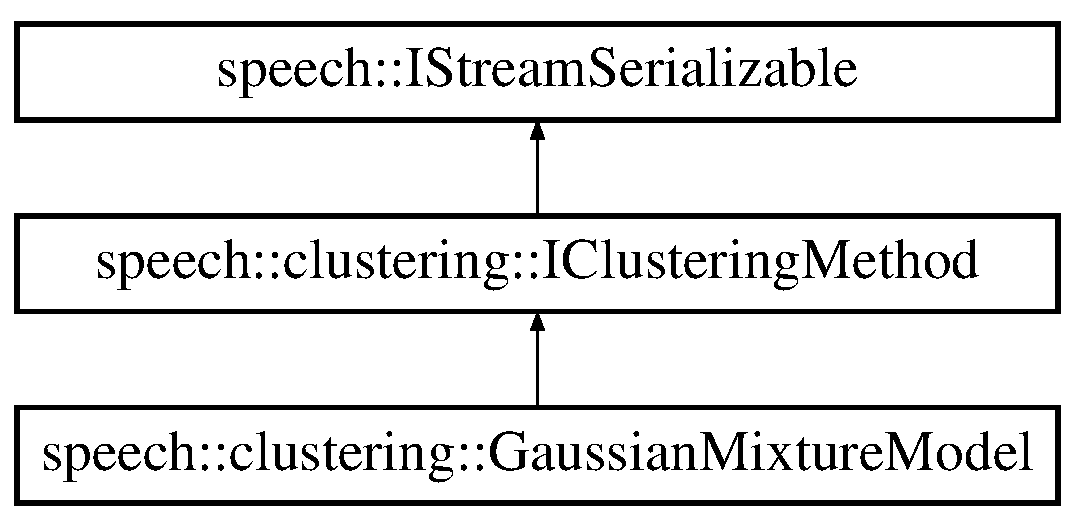
\includegraphics[height=3.000000cm]{classspeech_1_1clustering_1_1GaussianMixtureModel}
\end{center}
\end{figure}
\subsection*{Public Member Functions}
\begin{DoxyCompactItemize}
\item 
\hyperlink{classspeech_1_1clustering_1_1GaussianMixtureModel_a42140f884c132d4744d8ddd368073f9f}{Gaussian\+Mixture\+Model} (std\+::istream \&in)
\item 
\hyperlink{classspeech_1_1clustering_1_1GaussianMixtureModel_a0bebe61a309dc205019d319162b8ca03}{Gaussian\+Mixture\+Model} (int nb\+Clusters, int dimension)
\item 
\hyperlink{classspeech_1_1clustering_1_1GaussianMixtureModel_a3a82073609b479ff89e3e2f2a839a092}{$\sim$\+Gaussian\+Mixture\+Model} ()
\item 
virtual void \hyperlink{classspeech_1_1clustering_1_1GaussianMixtureModel_ab14e1843eb9412b32f918c909e19d1c5}{fit} (vector$<$ valarray$<$ double $>$$>$ \&vectors)
\item 
virtual int \hyperlink{classspeech_1_1clustering_1_1GaussianMixtureModel_a5ddd00a86bbc557b4beaf13760dc222f}{predict} (const valarray$<$ double $>$ \&vector)
\item 
virtual void \hyperlink{classspeech_1_1clustering_1_1GaussianMixtureModel_a51a73a7818e57e5b9e2ff6fbd25188f6}{serialize} (std\+::ostream \&out) const 
\end{DoxyCompactItemize}
\subsection*{Static Public Attributes}
\begin{DoxyCompactItemize}
\item 
\hypertarget{classspeech_1_1clustering_1_1GaussianMixtureModel_a5e24f49d58af9b9eededc498b5c63ad0}{static const uint32\+\_\+t {\bfseries T\+Y\+P\+E\+\_\+\+I\+D\+E\+N\+T\+I\+F\+I\+E\+R} = 0x00000002}\label{classspeech_1_1clustering_1_1GaussianMixtureModel_a5e24f49d58af9b9eededc498b5c63ad0}

\end{DoxyCompactItemize}


\subsection{Detailed Description}
Gaussian mixture model (G\+M\+M) implementation 

\subsection{Constructor \& Destructor Documentation}
\hypertarget{classspeech_1_1clustering_1_1GaussianMixtureModel_a42140f884c132d4744d8ddd368073f9f}{\index{speech\+::clustering\+::\+Gaussian\+Mixture\+Model@{speech\+::clustering\+::\+Gaussian\+Mixture\+Model}!Gaussian\+Mixture\+Model@{Gaussian\+Mixture\+Model}}
\index{Gaussian\+Mixture\+Model@{Gaussian\+Mixture\+Model}!speech\+::clustering\+::\+Gaussian\+Mixture\+Model@{speech\+::clustering\+::\+Gaussian\+Mixture\+Model}}
\subsubsection[{Gaussian\+Mixture\+Model}]{\setlength{\rightskip}{0pt plus 5cm}speech\+::clustering\+::\+Gaussian\+Mixture\+Model\+::\+Gaussian\+Mixture\+Model (
\begin{DoxyParamCaption}
\item[{std\+::istream \&}]{in}
\end{DoxyParamCaption}
)}}\label{classspeech_1_1clustering_1_1GaussianMixtureModel_a42140f884c132d4744d8ddd368073f9f}
Creates a Gaussian mixture model from the stream which contains serialized model. All parameters are loaded into the model, which can be then taught further. 
\begin{DoxyParams}{Parameters}
{\em in} & input stream \\
\hline
\end{DoxyParams}
\hypertarget{classspeech_1_1clustering_1_1GaussianMixtureModel_a0bebe61a309dc205019d319162b8ca03}{\index{speech\+::clustering\+::\+Gaussian\+Mixture\+Model@{speech\+::clustering\+::\+Gaussian\+Mixture\+Model}!Gaussian\+Mixture\+Model@{Gaussian\+Mixture\+Model}}
\index{Gaussian\+Mixture\+Model@{Gaussian\+Mixture\+Model}!speech\+::clustering\+::\+Gaussian\+Mixture\+Model@{speech\+::clustering\+::\+Gaussian\+Mixture\+Model}}
\subsubsection[{Gaussian\+Mixture\+Model}]{\setlength{\rightskip}{0pt plus 5cm}speech\+::clustering\+::\+Gaussian\+Mixture\+Model\+::\+Gaussian\+Mixture\+Model (
\begin{DoxyParamCaption}
\item[{int}]{nb\+Clusters, }
\item[{int}]{dimension}
\end{DoxyParamCaption}
)}}\label{classspeech_1_1clustering_1_1GaussianMixtureModel_a0bebe61a309dc205019d319162b8ca03}
Creates a Gaussian mixture model for given number of clusters and dimension of a single data vector. 
\begin{DoxyParams}{Parameters}
{\em nb\+Clusters} & number of clusters \\
\hline
{\em dimension} & single data vector dimension \\
\hline
\end{DoxyParams}
\hypertarget{classspeech_1_1clustering_1_1GaussianMixtureModel_a3a82073609b479ff89e3e2f2a839a092}{\index{speech\+::clustering\+::\+Gaussian\+Mixture\+Model@{speech\+::clustering\+::\+Gaussian\+Mixture\+Model}!````~Gaussian\+Mixture\+Model@{$\sim$\+Gaussian\+Mixture\+Model}}
\index{````~Gaussian\+Mixture\+Model@{$\sim$\+Gaussian\+Mixture\+Model}!speech\+::clustering\+::\+Gaussian\+Mixture\+Model@{speech\+::clustering\+::\+Gaussian\+Mixture\+Model}}
\subsubsection[{$\sim$\+Gaussian\+Mixture\+Model}]{\setlength{\rightskip}{0pt plus 5cm}speech\+::clustering\+::\+Gaussian\+Mixture\+Model\+::$\sim$\+Gaussian\+Mixture\+Model (
\begin{DoxyParamCaption}
{}
\end{DoxyParamCaption}
)}}\label{classspeech_1_1clustering_1_1GaussianMixtureModel_a3a82073609b479ff89e3e2f2a839a092}
Destructor 

\subsection{Member Function Documentation}
\hypertarget{classspeech_1_1clustering_1_1GaussianMixtureModel_ab14e1843eb9412b32f918c909e19d1c5}{\index{speech\+::clustering\+::\+Gaussian\+Mixture\+Model@{speech\+::clustering\+::\+Gaussian\+Mixture\+Model}!fit@{fit}}
\index{fit@{fit}!speech\+::clustering\+::\+Gaussian\+Mixture\+Model@{speech\+::clustering\+::\+Gaussian\+Mixture\+Model}}
\subsubsection[{fit}]{\setlength{\rightskip}{0pt plus 5cm}void speech\+::clustering\+::\+Gaussian\+Mixture\+Model\+::fit (
\begin{DoxyParamCaption}
\item[{vector$<$ valarray$<$ double $>$$>$ \&}]{vectors}
\end{DoxyParamCaption}
)\hspace{0.3cm}{\ttfamily [virtual]}}}\label{classspeech_1_1clustering_1_1GaussianMixtureModel_ab14e1843eb9412b32f918c909e19d1c5}
Trains the classifier using provided set of vectors 
\begin{DoxyParams}{Parameters}
{\em vectors} & collection of vectors used in a training phase \\
\hline
\end{DoxyParams}


Implements \hyperlink{classspeech_1_1clustering_1_1IClusteringMethod_ab9ec001a1f76be4793086cd8548ac886}{speech\+::clustering\+::\+I\+Clustering\+Method}.

\hypertarget{classspeech_1_1clustering_1_1GaussianMixtureModel_a5ddd00a86bbc557b4beaf13760dc222f}{\index{speech\+::clustering\+::\+Gaussian\+Mixture\+Model@{speech\+::clustering\+::\+Gaussian\+Mixture\+Model}!predict@{predict}}
\index{predict@{predict}!speech\+::clustering\+::\+Gaussian\+Mixture\+Model@{speech\+::clustering\+::\+Gaussian\+Mixture\+Model}}
\subsubsection[{predict}]{\setlength{\rightskip}{0pt plus 5cm}int speech\+::clustering\+::\+Gaussian\+Mixture\+Model\+::predict (
\begin{DoxyParamCaption}
\item[{const valarray$<$ double $>$ \&}]{vector}
\end{DoxyParamCaption}
)\hspace{0.3cm}{\ttfamily [virtual]}}}\label{classspeech_1_1clustering_1_1GaussianMixtureModel_a5ddd00a86bbc557b4beaf13760dc222f}
Predicts a label of given vector. It can be used only after training the classifier using fit method. 
\begin{DoxyParams}{Parameters}
{\em vector} & vector to be classified \\
\hline
\end{DoxyParams}


Implements \hyperlink{classspeech_1_1clustering_1_1IClusteringMethod_a47be2ed9fbe6792dcebc8fdcee7fa76e}{speech\+::clustering\+::\+I\+Clustering\+Method}.

\hypertarget{classspeech_1_1clustering_1_1GaussianMixtureModel_a51a73a7818e57e5b9e2ff6fbd25188f6}{\index{speech\+::clustering\+::\+Gaussian\+Mixture\+Model@{speech\+::clustering\+::\+Gaussian\+Mixture\+Model}!serialize@{serialize}}
\index{serialize@{serialize}!speech\+::clustering\+::\+Gaussian\+Mixture\+Model@{speech\+::clustering\+::\+Gaussian\+Mixture\+Model}}
\subsubsection[{serialize}]{\setlength{\rightskip}{0pt plus 5cm}void speech\+::clustering\+::\+Gaussian\+Mixture\+Model\+::serialize (
\begin{DoxyParamCaption}
\item[{std\+::ostream \&}]{out}
\end{DoxyParamCaption}
) const\hspace{0.3cm}{\ttfamily [virtual]}}}\label{classspeech_1_1clustering_1_1GaussianMixtureModel_a51a73a7818e57e5b9e2ff6fbd25188f6}
Writes an object to given stream 
\begin{DoxyParams}{Parameters}
{\em out} & output stream \\
\hline
\end{DoxyParams}


Implements \hyperlink{classspeech_1_1clustering_1_1IClusteringMethod_a9676e73a7c47d5383e9359850086249c}{speech\+::clustering\+::\+I\+Clustering\+Method}.



The documentation for this class was generated from the following files\+:\begin{DoxyCompactItemize}
\item 
/home/kacper/\+Projects/speech-\/recognition/src/speech/clustering/Gaussian\+Mixture\+Model.\+h\item 
/home/kacper/\+Projects/speech-\/recognition/src/speech/clustering/Gaussian\+Mixture\+Model.\+cpp\end{DoxyCompactItemize}

\hypertarget{classspeech_1_1transform_1_1window_1_1GaussWindow}{\section{speech\+:\+:transform\+:\+:window\+:\+:Gauss\+Window Class Reference}
\label{classspeech_1_1transform_1_1window_1_1GaussWindow}\index{speech\+::transform\+::window\+::\+Gauss\+Window@{speech\+::transform\+::window\+::\+Gauss\+Window}}
}
Inheritance diagram for speech\+:\+:transform\+:\+:window\+:\+:Gauss\+Window\+:\begin{figure}[H]
\begin{center}
\leavevmode
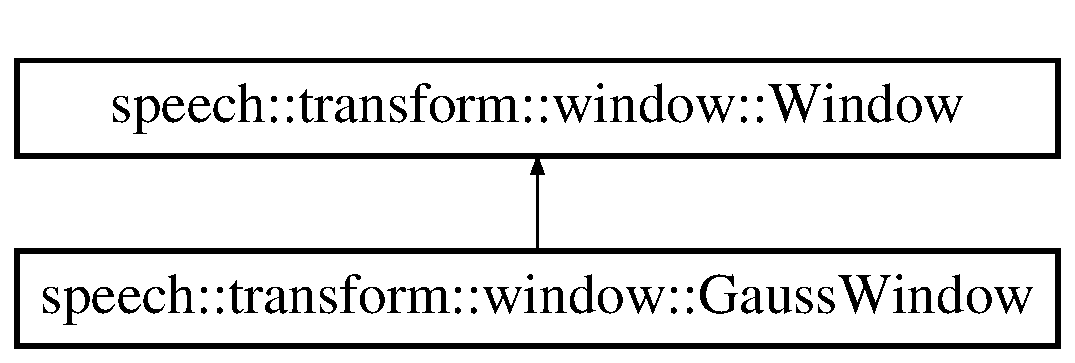
\includegraphics[height=2.000000cm]{classspeech_1_1transform_1_1window_1_1GaussWindow}
\end{center}
\end{figure}
\subsection*{Public Member Functions}
\begin{DoxyCompactItemize}
\item 
\hypertarget{classspeech_1_1transform_1_1window_1_1GaussWindow_ab9bb9cbbb5d8414652ccc2306445f5bc}{{\bfseries Gauss\+Window} (unsigned int window\+Size, double sigma)}\label{classspeech_1_1transform_1_1window_1_1GaussWindow_ab9bb9cbbb5d8414652ccc2306445f5bc}

\end{DoxyCompactItemize}
\subsection*{Protected Member Functions}
\begin{DoxyCompactItemize}
\item 
\hypertarget{classspeech_1_1transform_1_1window_1_1GaussWindow_a3cad13f188cdcebcdfe00df65a6b9e6e}{virtual const double {\bfseries get\+Window\+Multiplier} (unsigned int index)}\label{classspeech_1_1transform_1_1window_1_1GaussWindow_a3cad13f188cdcebcdfe00df65a6b9e6e}

\end{DoxyCompactItemize}


The documentation for this class was generated from the following files\+:\begin{DoxyCompactItemize}
\item 
/home/kacper/\+Projects/speech-\/recognition/src/speech/transform/window/Gauss\+Window.\+h\item 
/home/kacper/\+Projects/speech-\/recognition/src/speech/transform/window/Gauss\+Window.\+cpp\end{DoxyCompactItemize}

\hypertarget{classspeech_1_1HMMLexicon_1_1GMMLikelihoodFunction}{\section{speech\+:\+:H\+M\+M\+Lexicon\+:\+:G\+M\+M\+Likelihood\+Function Class Reference}
\label{classspeech_1_1HMMLexicon_1_1GMMLikelihoodFunction}\index{speech\+::\+H\+M\+M\+Lexicon\+::\+G\+M\+M\+Likelihood\+Function@{speech\+::\+H\+M\+M\+Lexicon\+::\+G\+M\+M\+Likelihood\+Function}}
}


{\ttfamily \#include $<$H\+M\+M\+Lexicon.\+h$>$}

\subsection*{Public Member Functions}
\begin{DoxyCompactItemize}
\item 
\hyperlink{classspeech_1_1HMMLexicon_1_1GMMLikelihoodFunction_a0398223855932fab00cce6ed3c7c9044}{G\+M\+M\+Likelihood\+Function} (unsigned int \hyperlink{classspeech_1_1HMMLexicon_1_1GMMLikelihoodFunction_aa163286d0699faf1dd14b01b6e118c13}{M}, unsigned int \hyperlink{classspeech_1_1HMMLexicon_1_1GMMLikelihoodFunction_a94b3da253b242046d0999c6138306fb3}{D})
\item 
double \hyperlink{classspeech_1_1HMMLexicon_1_1GMMLikelihoodFunction_a5f0bbd3150c1540c0fa12642890db2be}{operator()} (const valarray$<$ double $>$ \&observation)
\item 
double \hyperlink{classspeech_1_1HMMLexicon_1_1GMMLikelihoodFunction_aff059a88e4cd71d3c1e4aa2cba6d292d}{operator()} (unsigned int k, const valarray$<$ double $>$ \&observation)
\item 
const double \& \hyperlink{classspeech_1_1HMMLexicon_1_1GMMLikelihoodFunction_a7333805192ae53f09bb38978f9670a21}{get\+Weight} (unsigned int k) const 
\item 
const valarray$<$ double $>$ \& \hyperlink{classspeech_1_1HMMLexicon_1_1GMMLikelihoodFunction_a1d311f247c4b83d5f04ca7a4ed9a8ff0}{get\+Means} (unsigned int k) const 
\item 
const valarray$<$ double $>$ \& \hyperlink{classspeech_1_1HMMLexicon_1_1GMMLikelihoodFunction_a9ad16b9c22994013463956d647bd7d98}{get\+Variances} (unsigned int k) const 
\item 
void \hyperlink{classspeech_1_1HMMLexicon_1_1GMMLikelihoodFunction_ac5ee1801bfb91e86a2fa1526bb4d6c31}{set\+Weight} (int mixture, double weight)
\item 
void \hyperlink{classspeech_1_1HMMLexicon_1_1GMMLikelihoodFunction_ae7de73b5ab1d8082773450aeb012a56a}{set\+Mean} (int mixture, int dimension, double mean)
\item 
void \hyperlink{classspeech_1_1HMMLexicon_1_1GMMLikelihoodFunction_aa7dde74f2d993c09c649fb98294e300b}{set\+Means} (int mixture, valarray$<$ double $>$ \hyperlink{classspeech_1_1HMMLexicon_1_1GMMLikelihoodFunction_a81095daa04f62f40f9096c3f05bbedd7}{means})
\item 
void \hyperlink{classspeech_1_1HMMLexicon_1_1GMMLikelihoodFunction_ad0ea26f1757fc88599a91b42ce52d7f2}{set\+Variance} (int mixture, int dimension, double variance)
\item 
void \hyperlink{classspeech_1_1HMMLexicon_1_1GMMLikelihoodFunction_aa83c7519bd307ea5c47dcbdff381b602}{set\+Variances} (int mixture, valarray$<$ double $>$ \hyperlink{classspeech_1_1HMMLexicon_1_1GMMLikelihoodFunction_a9e996ef1a355aafa7143b5e5d2bf6b8a}{variances})
\end{DoxyCompactItemize}
\subsection*{Protected Attributes}
\begin{DoxyCompactItemize}
\item 
unsigned int \hyperlink{classspeech_1_1HMMLexicon_1_1GMMLikelihoodFunction_aa163286d0699faf1dd14b01b6e118c13}{M}
\item 
unsigned int \hyperlink{classspeech_1_1HMMLexicon_1_1GMMLikelihoodFunction_a94b3da253b242046d0999c6138306fb3}{D}
\item 
valarray$<$ double $>$ \hyperlink{classspeech_1_1HMMLexicon_1_1GMMLikelihoodFunction_aa3511faf53d4e9209d46a4af968ae4a7}{weights}
\item 
vector$<$ valarray$<$ double $>$ $>$ \hyperlink{classspeech_1_1HMMLexicon_1_1GMMLikelihoodFunction_a81095daa04f62f40f9096c3f05bbedd7}{means}
\item 
vector$<$ valarray$<$ double $>$ $>$ \hyperlink{classspeech_1_1HMMLexicon_1_1GMMLikelihoodFunction_a9e996ef1a355aafa7143b5e5d2bf6b8a}{variances}
\end{DoxyCompactItemize}


\subsection{Detailed Description}
Function of a likelihood approximating the distribution using Gaussian mixture model. 

\subsection{Constructor \& Destructor Documentation}
\hypertarget{classspeech_1_1HMMLexicon_1_1GMMLikelihoodFunction_a0398223855932fab00cce6ed3c7c9044}{\index{speech\+::\+H\+M\+M\+Lexicon\+::\+G\+M\+M\+Likelihood\+Function@{speech\+::\+H\+M\+M\+Lexicon\+::\+G\+M\+M\+Likelihood\+Function}!G\+M\+M\+Likelihood\+Function@{G\+M\+M\+Likelihood\+Function}}
\index{G\+M\+M\+Likelihood\+Function@{G\+M\+M\+Likelihood\+Function}!speech\+::\+H\+M\+M\+Lexicon\+::\+G\+M\+M\+Likelihood\+Function@{speech\+::\+H\+M\+M\+Lexicon\+::\+G\+M\+M\+Likelihood\+Function}}
\subsubsection[{G\+M\+M\+Likelihood\+Function}]{\setlength{\rightskip}{0pt plus 5cm}speech\+::\+H\+M\+M\+Lexicon\+::\+G\+M\+M\+Likelihood\+Function\+::\+G\+M\+M\+Likelihood\+Function (
\begin{DoxyParamCaption}
\item[{unsigned int}]{M, }
\item[{unsigned int}]{D}
\end{DoxyParamCaption}
)}}\label{classspeech_1_1HMMLexicon_1_1GMMLikelihoodFunction_a0398223855932fab00cce6ed3c7c9044}
Constructs an object representing function built from given number of multivariate Gaussians. 
\begin{DoxyParams}{Parameters}
{\em M} & number of Gaussians \\
\hline
{\em D} & dimensionality of a single input vector \\
\hline
\end{DoxyParams}


\subsection{Member Function Documentation}
\hypertarget{classspeech_1_1HMMLexicon_1_1GMMLikelihoodFunction_a1d311f247c4b83d5f04ca7a4ed9a8ff0}{\index{speech\+::\+H\+M\+M\+Lexicon\+::\+G\+M\+M\+Likelihood\+Function@{speech\+::\+H\+M\+M\+Lexicon\+::\+G\+M\+M\+Likelihood\+Function}!get\+Means@{get\+Means}}
\index{get\+Means@{get\+Means}!speech\+::\+H\+M\+M\+Lexicon\+::\+G\+M\+M\+Likelihood\+Function@{speech\+::\+H\+M\+M\+Lexicon\+::\+G\+M\+M\+Likelihood\+Function}}
\subsubsection[{get\+Means}]{\setlength{\rightskip}{0pt plus 5cm}const valarray$<$double$>$\& speech\+::\+H\+M\+M\+Lexicon\+::\+G\+M\+M\+Likelihood\+Function\+::get\+Means (
\begin{DoxyParamCaption}
\item[{unsigned int}]{k}
\end{DoxyParamCaption}
) const\hspace{0.3cm}{\ttfamily [inline]}}}\label{classspeech_1_1HMMLexicon_1_1GMMLikelihoodFunction_a1d311f247c4b83d5f04ca7a4ed9a8ff0}
Get means of selected mixture 
\begin{DoxyParams}{Parameters}
{\em k} & mixture number \\
\hline
\end{DoxyParams}
\hypertarget{classspeech_1_1HMMLexicon_1_1GMMLikelihoodFunction_a9ad16b9c22994013463956d647bd7d98}{\index{speech\+::\+H\+M\+M\+Lexicon\+::\+G\+M\+M\+Likelihood\+Function@{speech\+::\+H\+M\+M\+Lexicon\+::\+G\+M\+M\+Likelihood\+Function}!get\+Variances@{get\+Variances}}
\index{get\+Variances@{get\+Variances}!speech\+::\+H\+M\+M\+Lexicon\+::\+G\+M\+M\+Likelihood\+Function@{speech\+::\+H\+M\+M\+Lexicon\+::\+G\+M\+M\+Likelihood\+Function}}
\subsubsection[{get\+Variances}]{\setlength{\rightskip}{0pt plus 5cm}const valarray$<$double$>$\& speech\+::\+H\+M\+M\+Lexicon\+::\+G\+M\+M\+Likelihood\+Function\+::get\+Variances (
\begin{DoxyParamCaption}
\item[{unsigned int}]{k}
\end{DoxyParamCaption}
) const\hspace{0.3cm}{\ttfamily [inline]}}}\label{classspeech_1_1HMMLexicon_1_1GMMLikelihoodFunction_a9ad16b9c22994013463956d647bd7d98}
Get variances of selected mixture 
\begin{DoxyParams}{Parameters}
{\em k} & mixture number \\
\hline
\end{DoxyParams}
\hypertarget{classspeech_1_1HMMLexicon_1_1GMMLikelihoodFunction_a7333805192ae53f09bb38978f9670a21}{\index{speech\+::\+H\+M\+M\+Lexicon\+::\+G\+M\+M\+Likelihood\+Function@{speech\+::\+H\+M\+M\+Lexicon\+::\+G\+M\+M\+Likelihood\+Function}!get\+Weight@{get\+Weight}}
\index{get\+Weight@{get\+Weight}!speech\+::\+H\+M\+M\+Lexicon\+::\+G\+M\+M\+Likelihood\+Function@{speech\+::\+H\+M\+M\+Lexicon\+::\+G\+M\+M\+Likelihood\+Function}}
\subsubsection[{get\+Weight}]{\setlength{\rightskip}{0pt plus 5cm}const double\& speech\+::\+H\+M\+M\+Lexicon\+::\+G\+M\+M\+Likelihood\+Function\+::get\+Weight (
\begin{DoxyParamCaption}
\item[{unsigned int}]{k}
\end{DoxyParamCaption}
) const\hspace{0.3cm}{\ttfamily [inline]}}}\label{classspeech_1_1HMMLexicon_1_1GMMLikelihoodFunction_a7333805192ae53f09bb38978f9670a21}
Gets a weight of selected mixture 
\begin{DoxyParams}{Parameters}
{\em k} & mixture number \\
\hline
\end{DoxyParams}
\hypertarget{classspeech_1_1HMMLexicon_1_1GMMLikelihoodFunction_a5f0bbd3150c1540c0fa12642890db2be}{\index{speech\+::\+H\+M\+M\+Lexicon\+::\+G\+M\+M\+Likelihood\+Function@{speech\+::\+H\+M\+M\+Lexicon\+::\+G\+M\+M\+Likelihood\+Function}!operator()@{operator()}}
\index{operator()@{operator()}!speech\+::\+H\+M\+M\+Lexicon\+::\+G\+M\+M\+Likelihood\+Function@{speech\+::\+H\+M\+M\+Lexicon\+::\+G\+M\+M\+Likelihood\+Function}}
\subsubsection[{operator()}]{\setlength{\rightskip}{0pt plus 5cm}double speech\+::\+H\+M\+M\+Lexicon\+::\+G\+M\+M\+Likelihood\+Function\+::operator() (
\begin{DoxyParamCaption}
\item[{const valarray$<$ double $>$ \&}]{observation}
\end{DoxyParamCaption}
)}}\label{classspeech_1_1HMMLexicon_1_1GMMLikelihoodFunction_a5f0bbd3150c1540c0fa12642890db2be}
Calculates the probability of being in the state modelled by this likelihood function, when given vector was observed. 
\begin{DoxyParams}{Parameters}
{\em observation} & observed acoustic vector \\
\hline
\end{DoxyParams}
\begin{DoxyReturn}{Returns}
probability of being in this state 
\end{DoxyReturn}

\begin{DoxyExceptions}{Exceptions}
{\em std\+::out\+\_\+of\+\_\+range} & when given vector size is wrong \\
\hline
\end{DoxyExceptions}
\hypertarget{classspeech_1_1HMMLexicon_1_1GMMLikelihoodFunction_aff059a88e4cd71d3c1e4aa2cba6d292d}{\index{speech\+::\+H\+M\+M\+Lexicon\+::\+G\+M\+M\+Likelihood\+Function@{speech\+::\+H\+M\+M\+Lexicon\+::\+G\+M\+M\+Likelihood\+Function}!operator()@{operator()}}
\index{operator()@{operator()}!speech\+::\+H\+M\+M\+Lexicon\+::\+G\+M\+M\+Likelihood\+Function@{speech\+::\+H\+M\+M\+Lexicon\+::\+G\+M\+M\+Likelihood\+Function}}
\subsubsection[{operator()}]{\setlength{\rightskip}{0pt plus 5cm}double speech\+::\+H\+M\+M\+Lexicon\+::\+G\+M\+M\+Likelihood\+Function\+::operator() (
\begin{DoxyParamCaption}
\item[{unsigned int}]{k, }
\item[{const valarray$<$ double $>$ \&}]{observation}
\end{DoxyParamCaption}
)}}\label{classspeech_1_1HMMLexicon_1_1GMMLikelihoodFunction_aff059a88e4cd71d3c1e4aa2cba6d292d}
Calculates the probability of being in the state modelled by the k-\/th component of this likelihood function, when given vector was observed. 
\begin{DoxyParams}{Parameters}
{\em k} & mixture \\
\hline
{\em observation} & observed acoustic vector \\
\hline
\end{DoxyParams}
\begin{DoxyReturn}{Returns}
probability of being in this state 
\end{DoxyReturn}

\begin{DoxyExceptions}{Exceptions}
{\em std\+::out\+\_\+of\+\_\+range} & when given vector size is wrong \\
\hline
\end{DoxyExceptions}
\hypertarget{classspeech_1_1HMMLexicon_1_1GMMLikelihoodFunction_ae7de73b5ab1d8082773450aeb012a56a}{\index{speech\+::\+H\+M\+M\+Lexicon\+::\+G\+M\+M\+Likelihood\+Function@{speech\+::\+H\+M\+M\+Lexicon\+::\+G\+M\+M\+Likelihood\+Function}!set\+Mean@{set\+Mean}}
\index{set\+Mean@{set\+Mean}!speech\+::\+H\+M\+M\+Lexicon\+::\+G\+M\+M\+Likelihood\+Function@{speech\+::\+H\+M\+M\+Lexicon\+::\+G\+M\+M\+Likelihood\+Function}}
\subsubsection[{set\+Mean}]{\setlength{\rightskip}{0pt plus 5cm}void speech\+::\+H\+M\+M\+Lexicon\+::\+G\+M\+M\+Likelihood\+Function\+::set\+Mean (
\begin{DoxyParamCaption}
\item[{int}]{mixture, }
\item[{int}]{dimension, }
\item[{double}]{mean}
\end{DoxyParamCaption}
)\hspace{0.3cm}{\ttfamily [inline]}}}\label{classspeech_1_1HMMLexicon_1_1GMMLikelihoodFunction_ae7de73b5ab1d8082773450aeb012a56a}
Sets new mean of the selected Gaussian mixture and dimension 
\begin{DoxyParams}{Parameters}
{\em mixture} & \\
\hline
{\em dimension} & \\
\hline
{\em mean} & new mean \\
\hline
\end{DoxyParams}

\begin{DoxyExceptions}{Exceptions}
{\em std\+::out\+\_\+of\+\_\+range} & when selected dimension does not exist \\
\hline
\end{DoxyExceptions}
\hypertarget{classspeech_1_1HMMLexicon_1_1GMMLikelihoodFunction_aa7dde74f2d993c09c649fb98294e300b}{\index{speech\+::\+H\+M\+M\+Lexicon\+::\+G\+M\+M\+Likelihood\+Function@{speech\+::\+H\+M\+M\+Lexicon\+::\+G\+M\+M\+Likelihood\+Function}!set\+Means@{set\+Means}}
\index{set\+Means@{set\+Means}!speech\+::\+H\+M\+M\+Lexicon\+::\+G\+M\+M\+Likelihood\+Function@{speech\+::\+H\+M\+M\+Lexicon\+::\+G\+M\+M\+Likelihood\+Function}}
\subsubsection[{set\+Means}]{\setlength{\rightskip}{0pt plus 5cm}void speech\+::\+H\+M\+M\+Lexicon\+::\+G\+M\+M\+Likelihood\+Function\+::set\+Means (
\begin{DoxyParamCaption}
\item[{int}]{mixture, }
\item[{valarray$<$ double $>$}]{means}
\end{DoxyParamCaption}
)\hspace{0.3cm}{\ttfamily [inline]}}}\label{classspeech_1_1HMMLexicon_1_1GMMLikelihoodFunction_aa7dde74f2d993c09c649fb98294e300b}
Sets new means of the selected Gaussian mixture 
\begin{DoxyParams}{Parameters}
{\em mixture} & \\
\hline
{\em means} & new means \\
\hline
\end{DoxyParams}

\begin{DoxyExceptions}{Exceptions}
{\em std\+::out\+\_\+of\+\_\+range} & when given vector has wrong size \\
\hline
\end{DoxyExceptions}
\hypertarget{classspeech_1_1HMMLexicon_1_1GMMLikelihoodFunction_ad0ea26f1757fc88599a91b42ce52d7f2}{\index{speech\+::\+H\+M\+M\+Lexicon\+::\+G\+M\+M\+Likelihood\+Function@{speech\+::\+H\+M\+M\+Lexicon\+::\+G\+M\+M\+Likelihood\+Function}!set\+Variance@{set\+Variance}}
\index{set\+Variance@{set\+Variance}!speech\+::\+H\+M\+M\+Lexicon\+::\+G\+M\+M\+Likelihood\+Function@{speech\+::\+H\+M\+M\+Lexicon\+::\+G\+M\+M\+Likelihood\+Function}}
\subsubsection[{set\+Variance}]{\setlength{\rightskip}{0pt plus 5cm}void speech\+::\+H\+M\+M\+Lexicon\+::\+G\+M\+M\+Likelihood\+Function\+::set\+Variance (
\begin{DoxyParamCaption}
\item[{int}]{mixture, }
\item[{int}]{dimension, }
\item[{double}]{variance}
\end{DoxyParamCaption}
)\hspace{0.3cm}{\ttfamily [inline]}}}\label{classspeech_1_1HMMLexicon_1_1GMMLikelihoodFunction_ad0ea26f1757fc88599a91b42ce52d7f2}
Sets new variance of the selected Gaussian mixture and dimension 
\begin{DoxyParams}{Parameters}
{\em mixture} & \\
\hline
{\em dimension} & \\
\hline
{\em variance} & new variance \\
\hline
\end{DoxyParams}

\begin{DoxyExceptions}{Exceptions}
{\em std\+::out\+\_\+of\+\_\+range} & when selected dimension does not exist \\
\hline
\end{DoxyExceptions}
\hypertarget{classspeech_1_1HMMLexicon_1_1GMMLikelihoodFunction_aa83c7519bd307ea5c47dcbdff381b602}{\index{speech\+::\+H\+M\+M\+Lexicon\+::\+G\+M\+M\+Likelihood\+Function@{speech\+::\+H\+M\+M\+Lexicon\+::\+G\+M\+M\+Likelihood\+Function}!set\+Variances@{set\+Variances}}
\index{set\+Variances@{set\+Variances}!speech\+::\+H\+M\+M\+Lexicon\+::\+G\+M\+M\+Likelihood\+Function@{speech\+::\+H\+M\+M\+Lexicon\+::\+G\+M\+M\+Likelihood\+Function}}
\subsubsection[{set\+Variances}]{\setlength{\rightskip}{0pt plus 5cm}void speech\+::\+H\+M\+M\+Lexicon\+::\+G\+M\+M\+Likelihood\+Function\+::set\+Variances (
\begin{DoxyParamCaption}
\item[{int}]{mixture, }
\item[{valarray$<$ double $>$}]{variances}
\end{DoxyParamCaption}
)\hspace{0.3cm}{\ttfamily [inline]}}}\label{classspeech_1_1HMMLexicon_1_1GMMLikelihoodFunction_aa83c7519bd307ea5c47dcbdff381b602}
Sets new variances of the selected Gaussian mixture 
\begin{DoxyParams}{Parameters}
{\em mixture} & \\
\hline
{\em variances} & new variances \\
\hline
\end{DoxyParams}

\begin{DoxyExceptions}{Exceptions}
{\em std\+::out\+\_\+of\+\_\+range} & when selected dimension does not exist \\
\hline
\end{DoxyExceptions}
\hypertarget{classspeech_1_1HMMLexicon_1_1GMMLikelihoodFunction_ac5ee1801bfb91e86a2fa1526bb4d6c31}{\index{speech\+::\+H\+M\+M\+Lexicon\+::\+G\+M\+M\+Likelihood\+Function@{speech\+::\+H\+M\+M\+Lexicon\+::\+G\+M\+M\+Likelihood\+Function}!set\+Weight@{set\+Weight}}
\index{set\+Weight@{set\+Weight}!speech\+::\+H\+M\+M\+Lexicon\+::\+G\+M\+M\+Likelihood\+Function@{speech\+::\+H\+M\+M\+Lexicon\+::\+G\+M\+M\+Likelihood\+Function}}
\subsubsection[{set\+Weight}]{\setlength{\rightskip}{0pt plus 5cm}void speech\+::\+H\+M\+M\+Lexicon\+::\+G\+M\+M\+Likelihood\+Function\+::set\+Weight (
\begin{DoxyParamCaption}
\item[{int}]{mixture, }
\item[{double}]{weight}
\end{DoxyParamCaption}
)\hspace{0.3cm}{\ttfamily [inline]}}}\label{classspeech_1_1HMMLexicon_1_1GMMLikelihoodFunction_ac5ee1801bfb91e86a2fa1526bb4d6c31}
Sets new weight of the selected Gaussian mixture 
\begin{DoxyParams}{Parameters}
{\em mixture} & \\
\hline
{\em weight} & new weight \\
\hline
\end{DoxyParams}

\begin{DoxyExceptions}{Exceptions}
{\em std\+::out\+\_\+of\+\_\+range} & when selected dimension does not exist \\
\hline
\end{DoxyExceptions}


\subsection{Member Data Documentation}
\hypertarget{classspeech_1_1HMMLexicon_1_1GMMLikelihoodFunction_a94b3da253b242046d0999c6138306fb3}{\index{speech\+::\+H\+M\+M\+Lexicon\+::\+G\+M\+M\+Likelihood\+Function@{speech\+::\+H\+M\+M\+Lexicon\+::\+G\+M\+M\+Likelihood\+Function}!D@{D}}
\index{D@{D}!speech\+::\+H\+M\+M\+Lexicon\+::\+G\+M\+M\+Likelihood\+Function@{speech\+::\+H\+M\+M\+Lexicon\+::\+G\+M\+M\+Likelihood\+Function}}
\subsubsection[{D}]{\setlength{\rightskip}{0pt plus 5cm}unsigned int speech\+::\+H\+M\+M\+Lexicon\+::\+G\+M\+M\+Likelihood\+Function\+::\+D\hspace{0.3cm}{\ttfamily [protected]}}}\label{classspeech_1_1HMMLexicon_1_1GMMLikelihoodFunction_a94b3da253b242046d0999c6138306fb3}
Dimensionality of an acoustic input vector \hypertarget{classspeech_1_1HMMLexicon_1_1GMMLikelihoodFunction_aa163286d0699faf1dd14b01b6e118c13}{\index{speech\+::\+H\+M\+M\+Lexicon\+::\+G\+M\+M\+Likelihood\+Function@{speech\+::\+H\+M\+M\+Lexicon\+::\+G\+M\+M\+Likelihood\+Function}!M@{M}}
\index{M@{M}!speech\+::\+H\+M\+M\+Lexicon\+::\+G\+M\+M\+Likelihood\+Function@{speech\+::\+H\+M\+M\+Lexicon\+::\+G\+M\+M\+Likelihood\+Function}}
\subsubsection[{M}]{\setlength{\rightskip}{0pt plus 5cm}unsigned int speech\+::\+H\+M\+M\+Lexicon\+::\+G\+M\+M\+Likelihood\+Function\+::\+M\hspace{0.3cm}{\ttfamily [protected]}}}\label{classspeech_1_1HMMLexicon_1_1GMMLikelihoodFunction_aa163286d0699faf1dd14b01b6e118c13}
Number of mixtures \hypertarget{classspeech_1_1HMMLexicon_1_1GMMLikelihoodFunction_a81095daa04f62f40f9096c3f05bbedd7}{\index{speech\+::\+H\+M\+M\+Lexicon\+::\+G\+M\+M\+Likelihood\+Function@{speech\+::\+H\+M\+M\+Lexicon\+::\+G\+M\+M\+Likelihood\+Function}!means@{means}}
\index{means@{means}!speech\+::\+H\+M\+M\+Lexicon\+::\+G\+M\+M\+Likelihood\+Function@{speech\+::\+H\+M\+M\+Lexicon\+::\+G\+M\+M\+Likelihood\+Function}}
\subsubsection[{means}]{\setlength{\rightskip}{0pt plus 5cm}vector$<$valarray$<$double$>$ $>$ speech\+::\+H\+M\+M\+Lexicon\+::\+G\+M\+M\+Likelihood\+Function\+::means\hspace{0.3cm}{\ttfamily [protected]}}}\label{classspeech_1_1HMMLexicon_1_1GMMLikelihoodFunction_a81095daa04f62f40f9096c3f05bbedd7}
Means of mixtures (M x D) \hypertarget{classspeech_1_1HMMLexicon_1_1GMMLikelihoodFunction_a9e996ef1a355aafa7143b5e5d2bf6b8a}{\index{speech\+::\+H\+M\+M\+Lexicon\+::\+G\+M\+M\+Likelihood\+Function@{speech\+::\+H\+M\+M\+Lexicon\+::\+G\+M\+M\+Likelihood\+Function}!variances@{variances}}
\index{variances@{variances}!speech\+::\+H\+M\+M\+Lexicon\+::\+G\+M\+M\+Likelihood\+Function@{speech\+::\+H\+M\+M\+Lexicon\+::\+G\+M\+M\+Likelihood\+Function}}
\subsubsection[{variances}]{\setlength{\rightskip}{0pt plus 5cm}vector$<$valarray$<$double$>$ $>$ speech\+::\+H\+M\+M\+Lexicon\+::\+G\+M\+M\+Likelihood\+Function\+::variances\hspace{0.3cm}{\ttfamily [protected]}}}\label{classspeech_1_1HMMLexicon_1_1GMMLikelihoodFunction_a9e996ef1a355aafa7143b5e5d2bf6b8a}
Variances of mixtures (M x D) (could be matrices of covariances -\/ M x (D x D)) \hypertarget{classspeech_1_1HMMLexicon_1_1GMMLikelihoodFunction_aa3511faf53d4e9209d46a4af968ae4a7}{\index{speech\+::\+H\+M\+M\+Lexicon\+::\+G\+M\+M\+Likelihood\+Function@{speech\+::\+H\+M\+M\+Lexicon\+::\+G\+M\+M\+Likelihood\+Function}!weights@{weights}}
\index{weights@{weights}!speech\+::\+H\+M\+M\+Lexicon\+::\+G\+M\+M\+Likelihood\+Function@{speech\+::\+H\+M\+M\+Lexicon\+::\+G\+M\+M\+Likelihood\+Function}}
\subsubsection[{weights}]{\setlength{\rightskip}{0pt plus 5cm}valarray$<$double$>$ speech\+::\+H\+M\+M\+Lexicon\+::\+G\+M\+M\+Likelihood\+Function\+::weights\hspace{0.3cm}{\ttfamily [protected]}}}\label{classspeech_1_1HMMLexicon_1_1GMMLikelihoodFunction_aa3511faf53d4e9209d46a4af968ae4a7}
Mixtures' weights (M) 

The documentation for this class was generated from the following files\+:\begin{DoxyCompactItemize}
\item 
/home/kacper/\+Projects/speech-\/recognition/src/speech/H\+M\+M\+Lexicon.\+h\item 
/home/kacper/\+Projects/speech-\/recognition/src/speech/H\+M\+M\+Lexicon.\+cpp\end{DoxyCompactItemize}

\hypertarget{classspeech_1_1transform_1_1window_1_1HammingWindow}{\section{speech\+:\+:transform\+:\+:window\+:\+:Hamming\+Window Class Reference}
\label{classspeech_1_1transform_1_1window_1_1HammingWindow}\index{speech\+::transform\+::window\+::\+Hamming\+Window@{speech\+::transform\+::window\+::\+Hamming\+Window}}
}
Inheritance diagram for speech\+:\+:transform\+:\+:window\+:\+:Hamming\+Window\+:\begin{figure}[H]
\begin{center}
\leavevmode
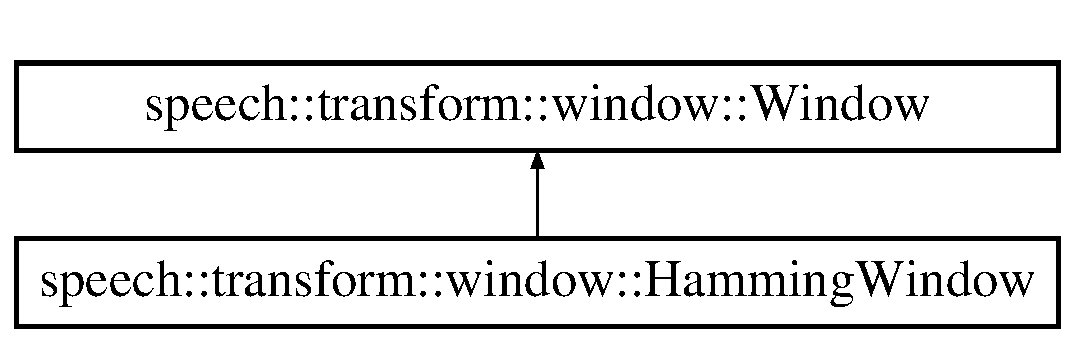
\includegraphics[height=2.000000cm]{classspeech_1_1transform_1_1window_1_1HammingWindow}
\end{center}
\end{figure}
\subsection*{Public Member Functions}
\begin{DoxyCompactItemize}
\item 
\hypertarget{classspeech_1_1transform_1_1window_1_1HammingWindow_a26e68fa1914f62cdecb055e2b4a0f9a9}{{\bfseries Hamming\+Window} (unsigned int window\+Size)}\label{classspeech_1_1transform_1_1window_1_1HammingWindow_a26e68fa1914f62cdecb055e2b4a0f9a9}

\end{DoxyCompactItemize}
\subsection*{Protected Member Functions}
\begin{DoxyCompactItemize}
\item 
\hypertarget{classspeech_1_1transform_1_1window_1_1HammingWindow_a1e6e7a7c10032ec1edda6589da318586}{virtual const double {\bfseries get\+Window\+Multiplier} (unsigned int index)}\label{classspeech_1_1transform_1_1window_1_1HammingWindow_a1e6e7a7c10032ec1edda6589da318586}

\end{DoxyCompactItemize}


The documentation for this class was generated from the following files\+:\begin{DoxyCompactItemize}
\item 
/home/kacper/\+Projects/speech-\/recognition/src/speech/transform/window/Hamming\+Window.\+h\item 
/home/kacper/\+Projects/speech-\/recognition/src/speech/transform/window/Hamming\+Window.\+cpp\end{DoxyCompactItemize}

\hypertarget{classspeech_1_1transform_1_1window_1_1HannWindow}{\section{speech\+:\+:transform\+:\+:window\+:\+:Hann\+Window Class Reference}
\label{classspeech_1_1transform_1_1window_1_1HannWindow}\index{speech\+::transform\+::window\+::\+Hann\+Window@{speech\+::transform\+::window\+::\+Hann\+Window}}
}
Inheritance diagram for speech\+:\+:transform\+:\+:window\+:\+:Hann\+Window\+:\begin{figure}[H]
\begin{center}
\leavevmode
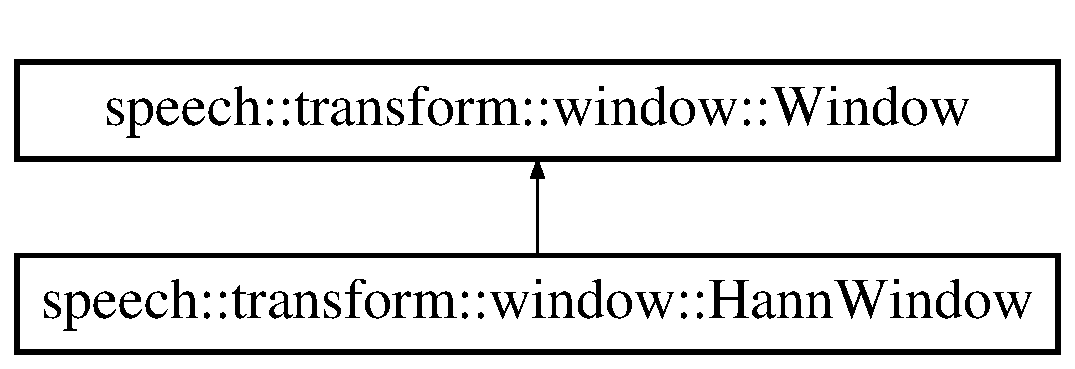
\includegraphics[height=2.000000cm]{classspeech_1_1transform_1_1window_1_1HannWindow}
\end{center}
\end{figure}
\subsection*{Public Member Functions}
\begin{DoxyCompactItemize}
\item 
\hypertarget{classspeech_1_1transform_1_1window_1_1HannWindow_af36a703d5b57bb3d5d01de187aabedc7}{{\bfseries Hann\+Window} (unsigned int window\+Size)}\label{classspeech_1_1transform_1_1window_1_1HannWindow_af36a703d5b57bb3d5d01de187aabedc7}

\end{DoxyCompactItemize}
\subsection*{Protected Member Functions}
\begin{DoxyCompactItemize}
\item 
\hypertarget{classspeech_1_1transform_1_1window_1_1HannWindow_add76ee5637f9c0ae3e830e409c013151}{virtual const double {\bfseries get\+Window\+Multiplier} (unsigned int index)}\label{classspeech_1_1transform_1_1window_1_1HannWindow_add76ee5637f9c0ae3e830e409c013151}

\end{DoxyCompactItemize}


The documentation for this class was generated from the following files\+:\begin{DoxyCompactItemize}
\item 
/home/kacper/\+Projects/speech-\/recognition/src/speech/transform/window/Hann\+Window.\+h\item 
/home/kacper/\+Projects/speech-\/recognition/src/speech/transform/window/Hann\+Window.\+cpp\end{DoxyCompactItemize}

\hypertarget{classspeech_1_1vectorizer_1_1HarmonicsVectorizer}{\section{speech\+:\+:vectorizer\+:\+:Harmonics\+Vectorizer$<$ Frame\+Type $>$ Class Template Reference}
\label{classspeech_1_1vectorizer_1_1HarmonicsVectorizer}\index{speech\+::vectorizer\+::\+Harmonics\+Vectorizer$<$ Frame\+Type $>$@{speech\+::vectorizer\+::\+Harmonics\+Vectorizer$<$ Frame\+Type $>$}}
}
Inheritance diagram for speech\+:\+:vectorizer\+:\+:Harmonics\+Vectorizer$<$ Frame\+Type $>$\+:\begin{figure}[H]
\begin{center}
\leavevmode
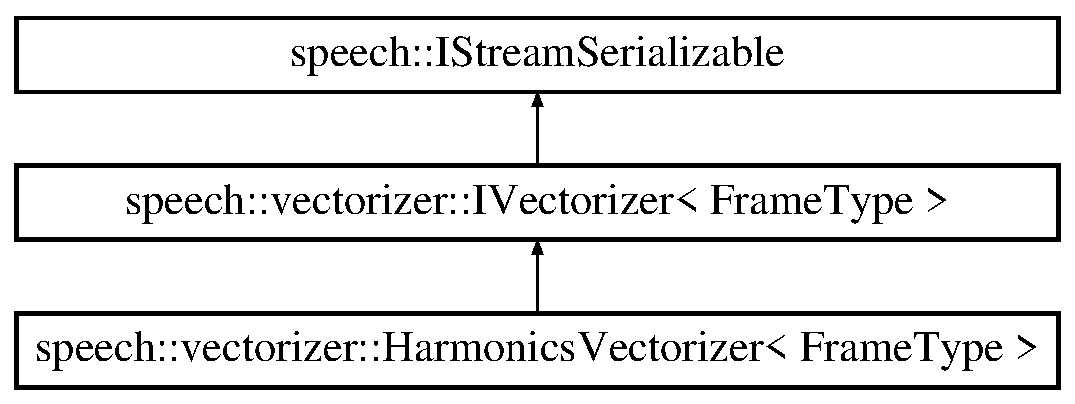
\includegraphics[height=3.000000cm]{classspeech_1_1vectorizer_1_1HarmonicsVectorizer}
\end{center}
\end{figure}
\subsection*{Public Member Functions}
\begin{DoxyCompactItemize}
\item 
\hyperlink{classspeech_1_1vectorizer_1_1HarmonicsVectorizer_ad0a68acf0931645d967de2e944f24809}{Harmonics\+Vectorizer} (int max\+Harmonics)
\item 
virtual std\+::valarray$<$ double $>$ \hyperlink{classspeech_1_1vectorizer_1_1HarmonicsVectorizer_a7f2d8f5d43c416ae95025d63c54d4385}{vectorize} (\hyperlink{classspeech_1_1raw__data_1_1FrequencySample}{Frequency\+Sample}$<$ Frame\+Type $>$ \&sample)
\item 
virtual void \hyperlink{classspeech_1_1vectorizer_1_1HarmonicsVectorizer_a6a9467047e5acbfd0fc4bf1e72679acf}{serialize} (std\+::ostream \&out) const 
\item 
virtual int \hyperlink{classspeech_1_1vectorizer_1_1HarmonicsVectorizer_aa6c06fb4864a9bd9e67675b6d836170f}{get\+Vector\+Size} () const 
\end{DoxyCompactItemize}
\subsection*{Additional Inherited Members}


\subsection{Constructor \& Destructor Documentation}
\hypertarget{classspeech_1_1vectorizer_1_1HarmonicsVectorizer_ad0a68acf0931645d967de2e944f24809}{\index{speech\+::vectorizer\+::\+Harmonics\+Vectorizer@{speech\+::vectorizer\+::\+Harmonics\+Vectorizer}!Harmonics\+Vectorizer@{Harmonics\+Vectorizer}}
\index{Harmonics\+Vectorizer@{Harmonics\+Vectorizer}!speech\+::vectorizer\+::\+Harmonics\+Vectorizer@{speech\+::vectorizer\+::\+Harmonics\+Vectorizer}}
\subsubsection[{Harmonics\+Vectorizer}]{\setlength{\rightskip}{0pt plus 5cm}template$<$typename Frame\+Type $>$ {\bf speech\+::vectorizer\+::\+Harmonics\+Vectorizer}$<$ Frame\+Type $>$\+::{\bf Harmonics\+Vectorizer} (
\begin{DoxyParamCaption}
\item[{int}]{max\+Harmonics}
\end{DoxyParamCaption}
)\hspace{0.3cm}{\ttfamily [inline]}}}\label{classspeech_1_1vectorizer_1_1HarmonicsVectorizer_ad0a68acf0931645d967de2e944f24809}
Creates a new vectorizer founding the harmonics of samples. 
\begin{DoxyParams}{Parameters}
{\em max\+Harmonics} & maximal number of the harmonics \\
\hline
\end{DoxyParams}


\subsection{Member Function Documentation}
\hypertarget{classspeech_1_1vectorizer_1_1HarmonicsVectorizer_aa6c06fb4864a9bd9e67675b6d836170f}{\index{speech\+::vectorizer\+::\+Harmonics\+Vectorizer@{speech\+::vectorizer\+::\+Harmonics\+Vectorizer}!get\+Vector\+Size@{get\+Vector\+Size}}
\index{get\+Vector\+Size@{get\+Vector\+Size}!speech\+::vectorizer\+::\+Harmonics\+Vectorizer@{speech\+::vectorizer\+::\+Harmonics\+Vectorizer}}
\subsubsection[{get\+Vector\+Size}]{\setlength{\rightskip}{0pt plus 5cm}template$<$typename Frame\+Type $>$ int {\bf speech\+::vectorizer\+::\+Harmonics\+Vectorizer}$<$ Frame\+Type $>$\+::get\+Vector\+Size (
\begin{DoxyParamCaption}
{}
\end{DoxyParamCaption}
) const\hspace{0.3cm}{\ttfamily [virtual]}}}\label{classspeech_1_1vectorizer_1_1HarmonicsVectorizer_aa6c06fb4864a9bd9e67675b6d836170f}
Gets the size of the output vector produced by the vectorizer.

\begin{DoxyReturn}{Returns}
size of the produced vector 
\end{DoxyReturn}


Implements \hyperlink{classspeech_1_1vectorizer_1_1IVectorizer_abe20529a1586c072783f42476ad7ab69}{speech\+::vectorizer\+::\+I\+Vectorizer$<$ Frame\+Type $>$}.

\hypertarget{classspeech_1_1vectorizer_1_1HarmonicsVectorizer_a6a9467047e5acbfd0fc4bf1e72679acf}{\index{speech\+::vectorizer\+::\+Harmonics\+Vectorizer@{speech\+::vectorizer\+::\+Harmonics\+Vectorizer}!serialize@{serialize}}
\index{serialize@{serialize}!speech\+::vectorizer\+::\+Harmonics\+Vectorizer@{speech\+::vectorizer\+::\+Harmonics\+Vectorizer}}
\subsubsection[{serialize}]{\setlength{\rightskip}{0pt plus 5cm}template$<$typename Frame\+Type $>$ void {\bf speech\+::vectorizer\+::\+Harmonics\+Vectorizer}$<$ Frame\+Type $>$\+::serialize (
\begin{DoxyParamCaption}
\item[{std\+::ostream \&}]{out}
\end{DoxyParamCaption}
) const\hspace{0.3cm}{\ttfamily [virtual]}}}\label{classspeech_1_1vectorizer_1_1HarmonicsVectorizer_a6a9467047e5acbfd0fc4bf1e72679acf}
Serializes the vectorizer into given stream. 
\begin{DoxyParams}{Parameters}
{\em out} & output stream \\
\hline
\end{DoxyParams}


Implements \hyperlink{classspeech_1_1vectorizer_1_1IVectorizer_aa8285bbd275c31ae1ce48d294400dea9}{speech\+::vectorizer\+::\+I\+Vectorizer$<$ Frame\+Type $>$}.

\hypertarget{classspeech_1_1vectorizer_1_1HarmonicsVectorizer_a7f2d8f5d43c416ae95025d63c54d4385}{\index{speech\+::vectorizer\+::\+Harmonics\+Vectorizer@{speech\+::vectorizer\+::\+Harmonics\+Vectorizer}!vectorize@{vectorize}}
\index{vectorize@{vectorize}!speech\+::vectorizer\+::\+Harmonics\+Vectorizer@{speech\+::vectorizer\+::\+Harmonics\+Vectorizer}}
\subsubsection[{vectorize}]{\setlength{\rightskip}{0pt plus 5cm}template$<$typename Frame\+Type $>$ std\+::valarray$<$ double $>$ {\bf speech\+::vectorizer\+::\+Harmonics\+Vectorizer}$<$ Frame\+Type $>$\+::vectorize (
\begin{DoxyParamCaption}
\item[{{\bf Frequency\+Sample}$<$ Frame\+Type $>$ \&}]{sample}
\end{DoxyParamCaption}
)\hspace{0.3cm}{\ttfamily [virtual]}}}\label{classspeech_1_1vectorizer_1_1HarmonicsVectorizer_a7f2d8f5d43c416ae95025d63c54d4385}
Projects given sample into feature space. Each vector needs to have exactly same size. 
\begin{DoxyParams}{Parameters}
{\em sample} & single sample to be vectorized\\
\hline
\end{DoxyParams}
\begin{DoxyReturn}{Returns}
the projection of vector in a feature space 
\end{DoxyReturn}


Implements \hyperlink{classspeech_1_1vectorizer_1_1IVectorizer_a00d2ba71ec5c447780ffb0a29bfc9085}{speech\+::vectorizer\+::\+I\+Vectorizer$<$ Frame\+Type $>$}.



The documentation for this class was generated from the following files\+:\begin{DoxyCompactItemize}
\item 
/home/kacper/\+Projects/speech-\/recognition/src/speech/vectorizer/Harmonics\+Vectorizer.\+h\item 
/home/kacper/\+Projects/speech-\/recognition/src/speech/vectorizer/Harmonics\+Vectorizer.\+cpp\end{DoxyCompactItemize}

\hypertarget{classspeech_1_1spelling_1_1HMM}{\section{speech\+:\+:spelling\+:\+:H\+M\+M Class Reference}
\label{classspeech_1_1spelling_1_1HMM}\index{speech\+::spelling\+::\+H\+M\+M@{speech\+::spelling\+::\+H\+M\+M}}
}
Inheritance diagram for speech\+:\+:spelling\+:\+:H\+M\+M\+:\begin{figure}[H]
\begin{center}
\leavevmode
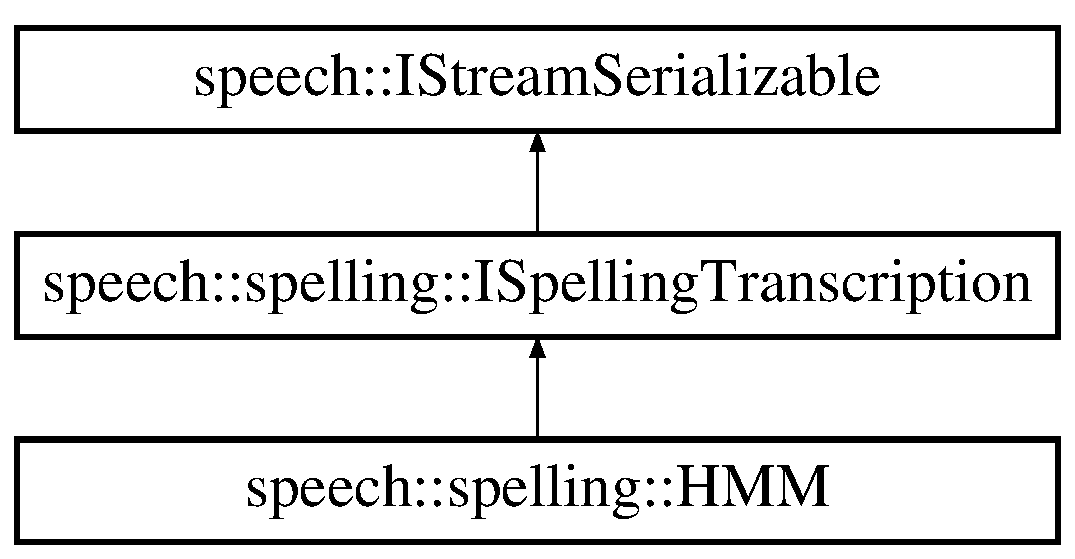
\includegraphics[height=3.000000cm]{classspeech_1_1spelling_1_1HMM}
\end{center}
\end{figure}
\subsection*{Public Member Functions}
\begin{DoxyCompactItemize}
\item 
\hypertarget{classspeech_1_1spelling_1_1HMM_ab6f28924b586c22b958bfac269b10f8b}{{\bfseries H\+M\+M} (int \+\_\+number\+Of\+Observations, int \+\_\+number\+Of\+States)}\label{classspeech_1_1spelling_1_1HMM_ab6f28924b586c22b958bfac269b10f8b}

\item 
\hypertarget{classspeech_1_1spelling_1_1HMM_a2165a35f20a11ff5942480a75471cafd}{{\bfseries H\+M\+M} (std\+::istream \&in)}\label{classspeech_1_1spelling_1_1HMM_a2165a35f20a11ff5942480a75471cafd}

\item 
\hypertarget{classspeech_1_1spelling_1_1HMM_ab7deb7571c4544319d268de72bfaa599}{{\bfseries H\+M\+M} (const std\+::vector$<$ int $>$ \&\+\_\+observations, const std\+::vector$<$ char $>$ \&\+\_\+states)}\label{classspeech_1_1spelling_1_1HMM_ab7deb7571c4544319d268de72bfaa599}

\item 
\hypertarget{classspeech_1_1spelling_1_1HMM_a84914784a009bf5ae2729afce623a770}{{\bfseries H\+M\+M} (int \+\_\+number\+Of\+Observations, const std\+::vector$<$ char $>$ \&\+\_\+states)}\label{classspeech_1_1spelling_1_1HMM_a84914784a009bf5ae2729afce623a770}

\item 
virtual void \hyperlink{classspeech_1_1spelling_1_1HMM_ae8a7d3797ef1f8d8ac3966db5500c552}{fit} (std\+::vector$<$ int $>$ \&phonems, const std\+::string \&spelling)
\item 
virtual std\+::string \hyperlink{classspeech_1_1spelling_1_1HMM_a01f7b06d7868bb526ca74526570dce21}{predict} (std\+::vector$<$ int $>$ phonems)
\item 
virtual void \hyperlink{classspeech_1_1spelling_1_1HMM_a225d39c70f721195c184e8af00ec3651}{serialize} (std\+::ostream \&out) const 
\end{DoxyCompactItemize}
\subsection*{Static Public Attributes}
\begin{DoxyCompactItemize}
\item 
\hypertarget{classspeech_1_1spelling_1_1HMM_af7d3303cd177e967b5820abee20e924e}{static const uint32\+\_\+t {\bfseries T\+Y\+P\+E\+\_\+\+I\+D\+E\+N\+T\+I\+F\+I\+E\+R} = 0x01000001}\label{classspeech_1_1spelling_1_1HMM_af7d3303cd177e967b5820abee20e924e}

\end{DoxyCompactItemize}
\subsection*{Protected Attributes}
\begin{DoxyCompactItemize}
\item 
\hypertarget{classspeech_1_1spelling_1_1HMM_a9a4067ac48b36326872616ef255d59b6}{int {\bfseries number\+Of\+Observations}}\label{classspeech_1_1spelling_1_1HMM_a9a4067ac48b36326872616ef255d59b6}

\item 
\hypertarget{classspeech_1_1spelling_1_1HMM_a1305b5ef325a521fc952c1d364d24bb8}{int {\bfseries number\+Of\+States}}\label{classspeech_1_1spelling_1_1HMM_a1305b5ef325a521fc952c1d364d24bb8}

\item 
\hypertarget{classspeech_1_1spelling_1_1HMM_a9730a77b166fbd1f676e3f9682d4026f}{std\+::vector$<$ int $>$ $\ast$ {\bfseries observations}}\label{classspeech_1_1spelling_1_1HMM_a9730a77b166fbd1f676e3f9682d4026f}

\item 
\hypertarget{classspeech_1_1spelling_1_1HMM_a28f1957d3c50355e6b5ad346b055c34c}{std\+::vector$<$ char $>$ $\ast$ {\bfseries states}}\label{classspeech_1_1spelling_1_1HMM_a28f1957d3c50355e6b5ad346b055c34c}

\item 
\hypertarget{classspeech_1_1spelling_1_1HMM_a81be786e67fdbff7acd61e36c86b2871}{shared\+\_\+ptr$<$ arma\+::mat $>$ {\bfseries transmission}}\label{classspeech_1_1spelling_1_1HMM_a81be786e67fdbff7acd61e36c86b2871}

\item 
\hypertarget{classspeech_1_1spelling_1_1HMM_afd8de0031aa51c58de818a6d25f96800}{shared\+\_\+ptr$<$ arma\+::mat $>$ {\bfseries emission}}\label{classspeech_1_1spelling_1_1HMM_afd8de0031aa51c58de818a6d25f96800}

\item 
\hypertarget{classspeech_1_1spelling_1_1HMM_a8bcb334bda85869b1b37b2a0a0a2185a}{shared\+\_\+ptr$<$ arma\+::vec $>$ {\bfseries pi}}\label{classspeech_1_1spelling_1_1HMM_a8bcb334bda85869b1b37b2a0a0a2185a}

\end{DoxyCompactItemize}


\subsection{Member Function Documentation}
\hypertarget{classspeech_1_1spelling_1_1HMM_ae8a7d3797ef1f8d8ac3966db5500c552}{\index{speech\+::spelling\+::\+H\+M\+M@{speech\+::spelling\+::\+H\+M\+M}!fit@{fit}}
\index{fit@{fit}!speech\+::spelling\+::\+H\+M\+M@{speech\+::spelling\+::\+H\+M\+M}}
\subsubsection[{fit}]{\setlength{\rightskip}{0pt plus 5cm}void speech\+::spelling\+::\+H\+M\+M\+::fit (
\begin{DoxyParamCaption}
\item[{std\+::vector$<$ int $>$ \&}]{phonems, }
\item[{const std\+::string \&}]{spelling}
\end{DoxyParamCaption}
)\hspace{0.3cm}{\ttfamily [virtual]}}}\label{classspeech_1_1spelling_1_1HMM_ae8a7d3797ef1f8d8ac3966db5500c552}
Add next example of the training data -\/ connections between sequence of phonems and sequence of letters. 

Implements \hyperlink{classspeech_1_1spelling_1_1ISpellingTranscription}{speech\+::spelling\+::\+I\+Spelling\+Transcription}.

\hypertarget{classspeech_1_1spelling_1_1HMM_a01f7b06d7868bb526ca74526570dce21}{\index{speech\+::spelling\+::\+H\+M\+M@{speech\+::spelling\+::\+H\+M\+M}!predict@{predict}}
\index{predict@{predict}!speech\+::spelling\+::\+H\+M\+M@{speech\+::spelling\+::\+H\+M\+M}}
\subsubsection[{predict}]{\setlength{\rightskip}{0pt plus 5cm}std\+::string speech\+::spelling\+::\+H\+M\+M\+::predict (
\begin{DoxyParamCaption}
\item[{std\+::vector$<$ int $>$}]{phonems}
\end{DoxyParamCaption}
)\hspace{0.3cm}{\ttfamily [virtual]}}}\label{classspeech_1_1spelling_1_1HMM_a01f7b06d7868bb526ca74526570dce21}
Perform a Viterbi algorithm to find most likely sequence of states which led to given observation. Phonems are considered to be observations, while letters of an alphabet are hidden states.

\begin{DoxyReturn}{Returns}
sequence of letters 
\end{DoxyReturn}


Implements \hyperlink{classspeech_1_1spelling_1_1ISpellingTranscription}{speech\+::spelling\+::\+I\+Spelling\+Transcription}.

\hypertarget{classspeech_1_1spelling_1_1HMM_a225d39c70f721195c184e8af00ec3651}{\index{speech\+::spelling\+::\+H\+M\+M@{speech\+::spelling\+::\+H\+M\+M}!serialize@{serialize}}
\index{serialize@{serialize}!speech\+::spelling\+::\+H\+M\+M@{speech\+::spelling\+::\+H\+M\+M}}
\subsubsection[{serialize}]{\setlength{\rightskip}{0pt plus 5cm}void speech\+::spelling\+::\+H\+M\+M\+::serialize (
\begin{DoxyParamCaption}
\item[{std\+::ostream \&}]{out}
\end{DoxyParamCaption}
) const\hspace{0.3cm}{\ttfamily [virtual]}}}\label{classspeech_1_1spelling_1_1HMM_a225d39c70f721195c184e8af00ec3651}
Writes an object to given stream 
\begin{DoxyParams}{Parameters}
{\em out} & output stream \\
\hline
\end{DoxyParams}


Implements \hyperlink{classspeech_1_1spelling_1_1ISpellingTranscription_a2ebd3da352eac002869c2f29ad890b16}{speech\+::spelling\+::\+I\+Spelling\+Transcription}.



The documentation for this class was generated from the following files\+:\begin{DoxyCompactItemize}
\item 
/home/kacper/\+Projects/speech-\/recognition/src/speech/spelling/H\+M\+M.\+h\item 
/home/kacper/\+Projects/speech-\/recognition/src/speech/spelling/H\+M\+M.\+cpp\end{DoxyCompactItemize}

\hypertarget{classspeech_1_1HMMLexicon}{\section{speech\+:\+:H\+M\+M\+Lexicon Class Reference}
\label{classspeech_1_1HMMLexicon}\index{speech\+::\+H\+M\+M\+Lexicon@{speech\+::\+H\+M\+M\+Lexicon}}
}


{\ttfamily \#include $<$H\+M\+M\+Lexicon.\+h$>$}

\subsection*{Classes}
\begin{DoxyCompactItemize}
\item 
class \hyperlink{classspeech_1_1HMMLexicon_1_1GMMLikelihoodFunction}{G\+M\+M\+Likelihood\+Function}
\item 
class \hyperlink{classspeech_1_1HMMLexicon_1_1MultivariateGaussianHMM}{Multivariate\+Gaussian\+H\+M\+M}
\end{DoxyCompactItemize}
\subsection*{Public Types}
\begin{DoxyCompactItemize}
\item 
\hypertarget{classspeech_1_1HMMLexicon_aa8d24ad3e9e92620ee2ce1f4cb783bad}{typedef vector$<$ valarray\\*
$<$ double $>$ $>$ {\bfseries Observation}}\label{classspeech_1_1HMMLexicon_aa8d24ad3e9e92620ee2ce1f4cb783bad}

\end{DoxyCompactItemize}
\subsection*{Public Member Functions}
\begin{DoxyCompactItemize}
\item 
\hyperlink{classspeech_1_1HMMLexicon_a720b99df01bd818f36cd9437ec83ce72}{H\+M\+M\+Lexicon} (int \hyperlink{classspeech_1_1HMMLexicon_a0e8247e6ee089aced3287ec0488e927b}{dimensionality}, unsigned int \hyperlink{classspeech_1_1HMMLexicon_a31c5dc5af41ea8a1f7ef825b2581b4d6}{gaussians}, std\+::shared\+\_\+ptr$<$ \hyperlink{classspeech_1_1initializer_1_1AbstractGaussianInitializer}{speech\+::initializer\+::\+Abstract\+Gaussian\+Initializer} $>$ \hyperlink{classspeech_1_1HMMLexicon_a12d561355a3c03df3d6500c422c1b821}{initializer}, unsigned int \hyperlink{classspeech_1_1HMMLexicon_a4f7a5e08c169ca9f5a389f25c6fc5972}{max\+Iterations}=100)
\item 
virtual \hyperlink{classspeech_1_1HMMLexicon_a07f9cfec2db8467b98c016b7e90f85d8}{$\sim$\+H\+M\+M\+Lexicon} ()
\item 
void \hyperlink{classspeech_1_1HMMLexicon_ae8b1812cf8ee22d64b87861f71f39ce2}{add\+Utterance} (Observation utterance, string transcription, string unit\+Separator=\char`\"{}$\vert$\char`\"{})
\item 
string \hyperlink{classspeech_1_1HMMLexicon_a6c9f0b864f71efd3946f760f3b955c6c}{predict} (const Observation \&observation)
\item 
std\+::map$<$ std\+::string, double $>$ \hyperlink{classspeech_1_1HMMLexicon_ab8d36b52d200a08213577aa72e85dbfe}{get\+Best\+Predictions} (const Observation \&observation, unsigned int N)
\item 
void \hyperlink{classspeech_1_1HMMLexicon_ab8858456fd0f64bf13fac21f2b30a317}{fit} ()
\item 
unsigned long \hyperlink{classspeech_1_1HMMLexicon_a834c97dbcac695589f117c2252101f88}{size} ()
\end{DoxyCompactItemize}
\subsection*{Protected Member Functions}
\begin{DoxyCompactItemize}
\item 
vector$<$ string $>$ \hyperlink{classspeech_1_1HMMLexicon_a36f384430151123b2a27b532fcb24d46}{split} (const string \&text, string \&separator)
\end{DoxyCompactItemize}
\subsection*{Protected Attributes}
\begin{DoxyCompactItemize}
\item 
int \hyperlink{classspeech_1_1HMMLexicon_a0e8247e6ee089aced3287ec0488e927b}{dimensionality}
\item 
unsigned int \hyperlink{classspeech_1_1HMMLexicon_a31c5dc5af41ea8a1f7ef825b2581b4d6}{gaussians}
\item 
std\+::shared\+\_\+ptr\\*
$<$ \hyperlink{classspeech_1_1initializer_1_1AbstractGaussianInitializer}{speech\+::initializer\+::\+Abstract\+Gaussian\+Initializer} $>$ \hyperlink{classspeech_1_1HMMLexicon_a12d561355a3c03df3d6500c422c1b821}{initializer}
\item 
unsigned int \hyperlink{classspeech_1_1HMMLexicon_a4f7a5e08c169ca9f5a389f25c6fc5972}{max\+Iterations}
\item 
map$<$ string, \\*
\hyperlink{classspeech_1_1HMMLexicon_1_1MultivariateGaussianHMM}{Multivariate\+Gaussian\+H\+M\+M} $\ast$ $>$ \hyperlink{classspeech_1_1HMMLexicon_aee3322e49c63383316eb46e489d81de9}{unit\+Models}
\end{DoxyCompactItemize}


\subsection{Detailed Description}
An acoustic model of the language built from H\+M\+Ms for each word / syllabe / phoneme from the dictionary. 

\subsection{Constructor \& Destructor Documentation}
\hypertarget{classspeech_1_1HMMLexicon_a720b99df01bd818f36cd9437ec83ce72}{\index{speech\+::\+H\+M\+M\+Lexicon@{speech\+::\+H\+M\+M\+Lexicon}!H\+M\+M\+Lexicon@{H\+M\+M\+Lexicon}}
\index{H\+M\+M\+Lexicon@{H\+M\+M\+Lexicon}!speech\+::\+H\+M\+M\+Lexicon@{speech\+::\+H\+M\+M\+Lexicon}}
\subsubsection[{H\+M\+M\+Lexicon}]{\setlength{\rightskip}{0pt plus 5cm}speech\+::\+H\+M\+M\+Lexicon\+::\+H\+M\+M\+Lexicon (
\begin{DoxyParamCaption}
\item[{int}]{dimensionality, }
\item[{unsigned int}]{gaussians, }
\item[{std\+::shared\+\_\+ptr$<$ {\bf speech\+::initializer\+::\+Abstract\+Gaussian\+Initializer} $>$}]{initializer, }
\item[{unsigned int}]{max\+Iterations = {\ttfamily 100}}
\end{DoxyParamCaption}
)}}\label{classspeech_1_1HMMLexicon_a720b99df01bd818f36cd9437ec83ce72}
Constructs an object with a custom initializer 
\begin{DoxyParams}{Parameters}
{\em dimensionality} & dimensionality of a single acoustic vector \\
\hline
{\em gaussians} & number of Gaussian mixtures in a single state of H\+M\+M \\
\hline
{\em initializer} & an instance of custom initializer \\
\hline
{\em max\+Iterations} & a maximum number of iterations to perform in model fitting \\
\hline
\end{DoxyParams}
\hypertarget{classspeech_1_1HMMLexicon_a07f9cfec2db8467b98c016b7e90f85d8}{\index{speech\+::\+H\+M\+M\+Lexicon@{speech\+::\+H\+M\+M\+Lexicon}!````~H\+M\+M\+Lexicon@{$\sim$\+H\+M\+M\+Lexicon}}
\index{````~H\+M\+M\+Lexicon@{$\sim$\+H\+M\+M\+Lexicon}!speech\+::\+H\+M\+M\+Lexicon@{speech\+::\+H\+M\+M\+Lexicon}}
\subsubsection[{$\sim$\+H\+M\+M\+Lexicon}]{\setlength{\rightskip}{0pt plus 5cm}speech\+::\+H\+M\+M\+Lexicon\+::$\sim$\+H\+M\+M\+Lexicon (
\begin{DoxyParamCaption}
{}
\end{DoxyParamCaption}
)\hspace{0.3cm}{\ttfamily [virtual]}}}\label{classspeech_1_1HMMLexicon_a07f9cfec2db8467b98c016b7e90f85d8}
Destructs the object 

\subsection{Member Function Documentation}
\hypertarget{classspeech_1_1HMMLexicon_ae8b1812cf8ee22d64b87861f71f39ce2}{\index{speech\+::\+H\+M\+M\+Lexicon@{speech\+::\+H\+M\+M\+Lexicon}!add\+Utterance@{add\+Utterance}}
\index{add\+Utterance@{add\+Utterance}!speech\+::\+H\+M\+M\+Lexicon@{speech\+::\+H\+M\+M\+Lexicon}}
\subsubsection[{add\+Utterance}]{\setlength{\rightskip}{0pt plus 5cm}void speech\+::\+H\+M\+M\+Lexicon\+::add\+Utterance (
\begin{DoxyParamCaption}
\item[{Observation}]{utterance, }
\item[{string}]{transcription, }
\item[{string}]{unit\+Separator = {\ttfamily \char`\"{}$\vert$\char`\"{}}}
\end{DoxyParamCaption}
)}}\label{classspeech_1_1HMMLexicon_ae8b1812cf8ee22d64b87861f71f39ce2}
Adds an acoustic observation of given text 
\begin{DoxyParams}{Parameters}
{\em utterance} & collection of acoustic observation vectors \\
\hline
{\em transcription} & text representing the observation \\
\hline
{\em unit\+Separator} & separator used for splitting the transcription \\
\hline
\end{DoxyParams}
\hypertarget{classspeech_1_1HMMLexicon_ab8858456fd0f64bf13fac21f2b30a317}{\index{speech\+::\+H\+M\+M\+Lexicon@{speech\+::\+H\+M\+M\+Lexicon}!fit@{fit}}
\index{fit@{fit}!speech\+::\+H\+M\+M\+Lexicon@{speech\+::\+H\+M\+M\+Lexicon}}
\subsubsection[{fit}]{\setlength{\rightskip}{0pt plus 5cm}void speech\+::\+H\+M\+M\+Lexicon\+::fit (
\begin{DoxyParamCaption}
{}
\end{DoxyParamCaption}
)}}\label{classspeech_1_1HMMLexicon_ab8858456fd0f64bf13fac21f2b30a317}
Fits the parameters of the lexicon \hypertarget{classspeech_1_1HMMLexicon_ab8d36b52d200a08213577aa72e85dbfe}{\index{speech\+::\+H\+M\+M\+Lexicon@{speech\+::\+H\+M\+M\+Lexicon}!get\+Best\+Predictions@{get\+Best\+Predictions}}
\index{get\+Best\+Predictions@{get\+Best\+Predictions}!speech\+::\+H\+M\+M\+Lexicon@{speech\+::\+H\+M\+M\+Lexicon}}
\subsubsection[{get\+Best\+Predictions}]{\setlength{\rightskip}{0pt plus 5cm}std\+::map$<$ std\+::string, double $>$ speech\+::\+H\+M\+M\+Lexicon\+::get\+Best\+Predictions (
\begin{DoxyParamCaption}
\item[{const Observation \&}]{observation, }
\item[{unsigned int}]{N}
\end{DoxyParamCaption}
)}}\label{classspeech_1_1HMMLexicon_ab8d36b52d200a08213577aa72e85dbfe}
Gets top N predictions of given utterance observation 
\begin{DoxyParams}{Parameters}
{\em observation} & collection of acoustic observation vectors \\
\hline
{\em N} & number of top predictions \\
\hline
\end{DoxyParams}
\begin{DoxyReturn}{Returns}
a collection of language units maximizing the probability of being observed with the log-\/likelihoods 
\end{DoxyReturn}
\hypertarget{classspeech_1_1HMMLexicon_a6c9f0b864f71efd3946f760f3b955c6c}{\index{speech\+::\+H\+M\+M\+Lexicon@{speech\+::\+H\+M\+M\+Lexicon}!predict@{predict}}
\index{predict@{predict}!speech\+::\+H\+M\+M\+Lexicon@{speech\+::\+H\+M\+M\+Lexicon}}
\subsubsection[{predict}]{\setlength{\rightskip}{0pt plus 5cm}string speech\+::\+H\+M\+M\+Lexicon\+::predict (
\begin{DoxyParamCaption}
\item[{const Observation \&}]{observation}
\end{DoxyParamCaption}
)}}\label{classspeech_1_1HMMLexicon_a6c9f0b864f71efd3946f760f3b955c6c}
Predicts a word which maximizes the probability of being observed in given observation 
\begin{DoxyParams}{Parameters}
{\em observation} & collection of acoustic observation vectors \\
\hline
\end{DoxyParams}
\begin{DoxyReturn}{Returns}
a language unit maximizing the probability of being observed 
\end{DoxyReturn}
\hypertarget{classspeech_1_1HMMLexicon_a834c97dbcac695589f117c2252101f88}{\index{speech\+::\+H\+M\+M\+Lexicon@{speech\+::\+H\+M\+M\+Lexicon}!size@{size}}
\index{size@{size}!speech\+::\+H\+M\+M\+Lexicon@{speech\+::\+H\+M\+M\+Lexicon}}
\subsubsection[{size}]{\setlength{\rightskip}{0pt plus 5cm}unsigned long speech\+::\+H\+M\+M\+Lexicon\+::size (
\begin{DoxyParamCaption}
{}
\end{DoxyParamCaption}
)\hspace{0.3cm}{\ttfamily [inline]}}}\label{classspeech_1_1HMMLexicon_a834c97dbcac695589f117c2252101f88}
Gets number of the unit models \begin{DoxyReturn}{Returns}
number of H\+M\+Ms 
\end{DoxyReturn}
\hypertarget{classspeech_1_1HMMLexicon_a36f384430151123b2a27b532fcb24d46}{\index{speech\+::\+H\+M\+M\+Lexicon@{speech\+::\+H\+M\+M\+Lexicon}!split@{split}}
\index{split@{split}!speech\+::\+H\+M\+M\+Lexicon@{speech\+::\+H\+M\+M\+Lexicon}}
\subsubsection[{split}]{\setlength{\rightskip}{0pt plus 5cm}vector$<$string$>$ speech\+::\+H\+M\+M\+Lexicon\+::split (
\begin{DoxyParamCaption}
\item[{const string \&}]{text, }
\item[{string \&}]{separator}
\end{DoxyParamCaption}
)\hspace{0.3cm}{\ttfamily [inline]}, {\ttfamily [protected]}}}\label{classspeech_1_1HMMLexicon_a36f384430151123b2a27b532fcb24d46}
Splits given string using given separator 
\begin{DoxyParams}{Parameters}
{\em text} & \\
\hline
{\em separator} & \\
\hline
\end{DoxyParams}
\begin{DoxyReturn}{Returns}
list of chunks 
\end{DoxyReturn}


\subsection{Member Data Documentation}
\hypertarget{classspeech_1_1HMMLexicon_a0e8247e6ee089aced3287ec0488e927b}{\index{speech\+::\+H\+M\+M\+Lexicon@{speech\+::\+H\+M\+M\+Lexicon}!dimensionality@{dimensionality}}
\index{dimensionality@{dimensionality}!speech\+::\+H\+M\+M\+Lexicon@{speech\+::\+H\+M\+M\+Lexicon}}
\subsubsection[{dimensionality}]{\setlength{\rightskip}{0pt plus 5cm}int speech\+::\+H\+M\+M\+Lexicon\+::dimensionality\hspace{0.3cm}{\ttfamily [protected]}}}\label{classspeech_1_1HMMLexicon_a0e8247e6ee089aced3287ec0488e927b}
Dimensionality of a single data vector \hypertarget{classspeech_1_1HMMLexicon_a31c5dc5af41ea8a1f7ef825b2581b4d6}{\index{speech\+::\+H\+M\+M\+Lexicon@{speech\+::\+H\+M\+M\+Lexicon}!gaussians@{gaussians}}
\index{gaussians@{gaussians}!speech\+::\+H\+M\+M\+Lexicon@{speech\+::\+H\+M\+M\+Lexicon}}
\subsubsection[{gaussians}]{\setlength{\rightskip}{0pt plus 5cm}unsigned int speech\+::\+H\+M\+M\+Lexicon\+::gaussians\hspace{0.3cm}{\ttfamily [protected]}}}\label{classspeech_1_1HMMLexicon_a31c5dc5af41ea8a1f7ef825b2581b4d6}
Number of mixture Gaussians used for the probability approximation \hypertarget{classspeech_1_1HMMLexicon_a12d561355a3c03df3d6500c422c1b821}{\index{speech\+::\+H\+M\+M\+Lexicon@{speech\+::\+H\+M\+M\+Lexicon}!initializer@{initializer}}
\index{initializer@{initializer}!speech\+::\+H\+M\+M\+Lexicon@{speech\+::\+H\+M\+M\+Lexicon}}
\subsubsection[{initializer}]{\setlength{\rightskip}{0pt plus 5cm}std\+::shared\+\_\+ptr$<${\bf speech\+::initializer\+::\+Abstract\+Gaussian\+Initializer}$>$ speech\+::\+H\+M\+M\+Lexicon\+::initializer\hspace{0.3cm}{\ttfamily [protected]}}}\label{classspeech_1_1HMMLexicon_a12d561355a3c03df3d6500c422c1b821}
Initializer of the Gaussian mixtures \hypertarget{classspeech_1_1HMMLexicon_a4f7a5e08c169ca9f5a389f25c6fc5972}{\index{speech\+::\+H\+M\+M\+Lexicon@{speech\+::\+H\+M\+M\+Lexicon}!max\+Iterations@{max\+Iterations}}
\index{max\+Iterations@{max\+Iterations}!speech\+::\+H\+M\+M\+Lexicon@{speech\+::\+H\+M\+M\+Lexicon}}
\subsubsection[{max\+Iterations}]{\setlength{\rightskip}{0pt plus 5cm}unsigned int speech\+::\+H\+M\+M\+Lexicon\+::max\+Iterations\hspace{0.3cm}{\ttfamily [protected]}}}\label{classspeech_1_1HMMLexicon_a4f7a5e08c169ca9f5a389f25c6fc5972}
Max iterations in a fitting phase \hypertarget{classspeech_1_1HMMLexicon_aee3322e49c63383316eb46e489d81de9}{\index{speech\+::\+H\+M\+M\+Lexicon@{speech\+::\+H\+M\+M\+Lexicon}!unit\+Models@{unit\+Models}}
\index{unit\+Models@{unit\+Models}!speech\+::\+H\+M\+M\+Lexicon@{speech\+::\+H\+M\+M\+Lexicon}}
\subsubsection[{unit\+Models}]{\setlength{\rightskip}{0pt plus 5cm}map$<$string, {\bf Multivariate\+Gaussian\+H\+M\+M} $\ast$$>$ speech\+::\+H\+M\+M\+Lexicon\+::unit\+Models\hspace{0.3cm}{\ttfamily [protected]}}}\label{classspeech_1_1HMMLexicon_aee3322e49c63383316eb46e489d81de9}
Collection of Hidden Markov Models, each one represents a single language unit 

The documentation for this class was generated from the following files\+:\begin{DoxyCompactItemize}
\item 
/home/kacper/\+Projects/speech-\/recognition/src/speech/H\+M\+M\+Lexicon.\+h\item 
/home/kacper/\+Projects/speech-\/recognition/src/speech/H\+M\+M\+Lexicon.\+cpp\end{DoxyCompactItemize}

\hypertarget{classspeech_1_1clustering_1_1IClusteringMethod}{\section{speech\+:\+:clustering\+:\+:I\+Clustering\+Method Class Reference}
\label{classspeech_1_1clustering_1_1IClusteringMethod}\index{speech\+::clustering\+::\+I\+Clustering\+Method@{speech\+::clustering\+::\+I\+Clustering\+Method}}
}


{\ttfamily \#include $<$I\+Clustering\+Method.\+h$>$}

Inheritance diagram for speech\+:\+:clustering\+:\+:I\+Clustering\+Method\+:\begin{figure}[H]
\begin{center}
\leavevmode
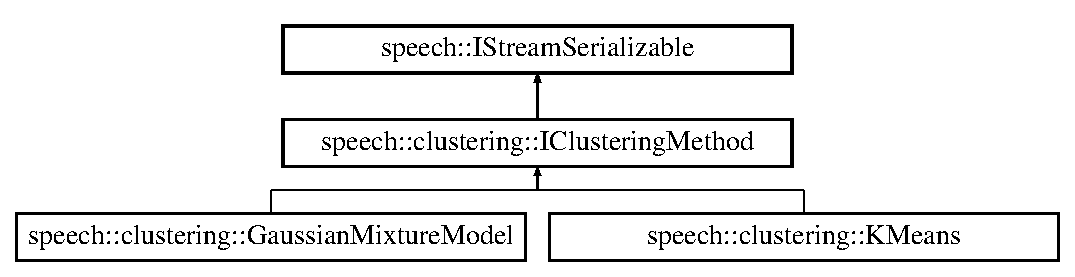
\includegraphics[height=3.000000cm]{classspeech_1_1clustering_1_1IClusteringMethod}
\end{center}
\end{figure}
\subsection*{Public Member Functions}
\begin{DoxyCompactItemize}
\item 
virtual void \hyperlink{classspeech_1_1clustering_1_1IClusteringMethod_ab9ec001a1f76be4793086cd8548ac886}{fit} (vector$<$ valarray$<$ double $>$$>$ \&vectors)=0
\item 
virtual int \hyperlink{classspeech_1_1clustering_1_1IClusteringMethod_a47be2ed9fbe6792dcebc8fdcee7fa76e}{predict} (const valarray$<$ double $>$ \&vector)=0
\item 
virtual void \hyperlink{classspeech_1_1clustering_1_1IClusteringMethod_a9676e73a7c47d5383e9359850086249c}{serialize} (std\+::ostream \&out) const =0
\end{DoxyCompactItemize}


\subsection{Detailed Description}
This is an interface for all clustering methods 

\subsection{Member Function Documentation}
\hypertarget{classspeech_1_1clustering_1_1IClusteringMethod_ab9ec001a1f76be4793086cd8548ac886}{\index{speech\+::clustering\+::\+I\+Clustering\+Method@{speech\+::clustering\+::\+I\+Clustering\+Method}!fit@{fit}}
\index{fit@{fit}!speech\+::clustering\+::\+I\+Clustering\+Method@{speech\+::clustering\+::\+I\+Clustering\+Method}}
\subsubsection[{fit}]{\setlength{\rightskip}{0pt plus 5cm}virtual void speech\+::clustering\+::\+I\+Clustering\+Method\+::fit (
\begin{DoxyParamCaption}
\item[{vector$<$ valarray$<$ double $>$$>$ \&}]{vectors}
\end{DoxyParamCaption}
)\hspace{0.3cm}{\ttfamily [pure virtual]}}}\label{classspeech_1_1clustering_1_1IClusteringMethod_ab9ec001a1f76be4793086cd8548ac886}
Trains the classifier using provided set of vectors 
\begin{DoxyParams}{Parameters}
{\em vectors} & collection of vectors used in a training phase \\
\hline
\end{DoxyParams}


Implemented in \hyperlink{classspeech_1_1clustering_1_1KMeans_a53a00478141ceee40366602a85e31ff4}{speech\+::clustering\+::\+K\+Means}, and \hyperlink{classspeech_1_1clustering_1_1GaussianMixtureModel_ab14e1843eb9412b32f918c909e19d1c5}{speech\+::clustering\+::\+Gaussian\+Mixture\+Model}.

\hypertarget{classspeech_1_1clustering_1_1IClusteringMethod_a47be2ed9fbe6792dcebc8fdcee7fa76e}{\index{speech\+::clustering\+::\+I\+Clustering\+Method@{speech\+::clustering\+::\+I\+Clustering\+Method}!predict@{predict}}
\index{predict@{predict}!speech\+::clustering\+::\+I\+Clustering\+Method@{speech\+::clustering\+::\+I\+Clustering\+Method}}
\subsubsection[{predict}]{\setlength{\rightskip}{0pt plus 5cm}virtual int speech\+::clustering\+::\+I\+Clustering\+Method\+::predict (
\begin{DoxyParamCaption}
\item[{const valarray$<$ double $>$ \&}]{vector}
\end{DoxyParamCaption}
)\hspace{0.3cm}{\ttfamily [pure virtual]}}}\label{classspeech_1_1clustering_1_1IClusteringMethod_a47be2ed9fbe6792dcebc8fdcee7fa76e}
Predicts a label of given vector. It can be used only after training the classifier using fit method. 
\begin{DoxyParams}{Parameters}
{\em vector} & vector to be classified \\
\hline
\end{DoxyParams}


Implemented in \hyperlink{classspeech_1_1clustering_1_1KMeans_a6b87bc8e097b0933220b7083ec846325}{speech\+::clustering\+::\+K\+Means}, and \hyperlink{classspeech_1_1clustering_1_1GaussianMixtureModel_a5ddd00a86bbc557b4beaf13760dc222f}{speech\+::clustering\+::\+Gaussian\+Mixture\+Model}.

\hypertarget{classspeech_1_1clustering_1_1IClusteringMethod_a9676e73a7c47d5383e9359850086249c}{\index{speech\+::clustering\+::\+I\+Clustering\+Method@{speech\+::clustering\+::\+I\+Clustering\+Method}!serialize@{serialize}}
\index{serialize@{serialize}!speech\+::clustering\+::\+I\+Clustering\+Method@{speech\+::clustering\+::\+I\+Clustering\+Method}}
\subsubsection[{serialize}]{\setlength{\rightskip}{0pt plus 5cm}virtual void speech\+::clustering\+::\+I\+Clustering\+Method\+::serialize (
\begin{DoxyParamCaption}
\item[{std\+::ostream \&}]{out}
\end{DoxyParamCaption}
) const\hspace{0.3cm}{\ttfamily [pure virtual]}}}\label{classspeech_1_1clustering_1_1IClusteringMethod_a9676e73a7c47d5383e9359850086249c}
Writes an object to given stream 
\begin{DoxyParams}{Parameters}
{\em out} & output stream \\
\hline
\end{DoxyParams}


Implements \hyperlink{classspeech_1_1IStreamSerializable_a891561ebe3e4eb5411e613b28bc2c982}{speech\+::\+I\+Stream\+Serializable}.



Implemented in \hyperlink{classspeech_1_1clustering_1_1KMeans_a47ba455f6996f45a1f61cde7e736e254}{speech\+::clustering\+::\+K\+Means}, and \hyperlink{classspeech_1_1clustering_1_1GaussianMixtureModel_a51a73a7818e57e5b9e2ff6fbd25188f6}{speech\+::clustering\+::\+Gaussian\+Mixture\+Model}.



The documentation for this class was generated from the following file\+:\begin{DoxyCompactItemize}
\item 
/home/kacper/\+Projects/speech-\/recognition/src/speech/clustering/I\+Clustering\+Method.\+h\end{DoxyCompactItemize}

\hypertarget{classspeech_1_1raw__data_1_1filtering_1_1IDataSampleFilter}{\section{speech\+:\+:raw\+\_\+data\+:\+:filtering\+:\+:I\+Data\+Sample\+Filter$<$ Frame\+Type $>$ Class Template Reference}
\label{classspeech_1_1raw__data_1_1filtering_1_1IDataSampleFilter}\index{speech\+::raw\+\_\+data\+::filtering\+::\+I\+Data\+Sample\+Filter$<$ Frame\+Type $>$@{speech\+::raw\+\_\+data\+::filtering\+::\+I\+Data\+Sample\+Filter$<$ Frame\+Type $>$}}
}
Inheritance diagram for speech\+:\+:raw\+\_\+data\+:\+:filtering\+:\+:I\+Data\+Sample\+Filter$<$ Frame\+Type $>$\+:\begin{figure}[H]
\begin{center}
\leavevmode
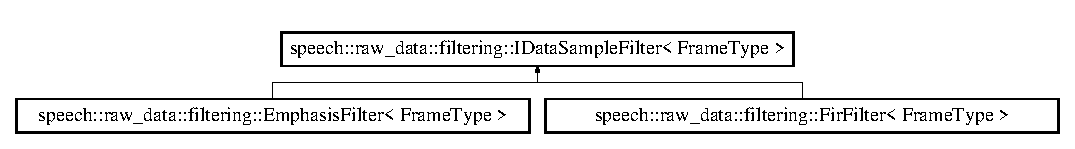
\includegraphics[height=1.555556cm]{classspeech_1_1raw__data_1_1filtering_1_1IDataSampleFilter}
\end{center}
\end{figure}
\subsection*{Public Member Functions}
\begin{DoxyCompactItemize}
\item 
\hypertarget{classspeech_1_1raw__data_1_1filtering_1_1IDataSampleFilter_a4f4f5b84b49c48075e7b6f7072067312}{virtual \hyperlink{classspeech_1_1raw__data_1_1DataSample}{Data\+Sample}$<$ Frame\+Type $>$ {\bfseries filter} (const \hyperlink{classspeech_1_1raw__data_1_1DataSample}{Data\+Sample}$<$ Frame\+Type $>$ \&sample)=0}\label{classspeech_1_1raw__data_1_1filtering_1_1IDataSampleFilter_a4f4f5b84b49c48075e7b6f7072067312}

\end{DoxyCompactItemize}


The documentation for this class was generated from the following file\+:\begin{DoxyCompactItemize}
\item 
/home/kacper/\+Projects/speech-\/recognition/src/speech/raw\+\_\+data/filtering/I\+Data\+Sample\+Filter.\+h\end{DoxyCompactItemize}

\hypertarget{classspeech_1_1detector_1_1IDetector}{\section{speech\+:\+:detector\+:\+:I\+Detector$<$ Frame\+Type $>$ Class Template Reference}
\label{classspeech_1_1detector_1_1IDetector}\index{speech\+::detector\+::\+I\+Detector$<$ Frame\+Type $>$@{speech\+::detector\+::\+I\+Detector$<$ Frame\+Type $>$}}
}
Inheritance diagram for speech\+:\+:detector\+:\+:I\+Detector$<$ Frame\+Type $>$\+:\begin{figure}[H]
\begin{center}
\leavevmode
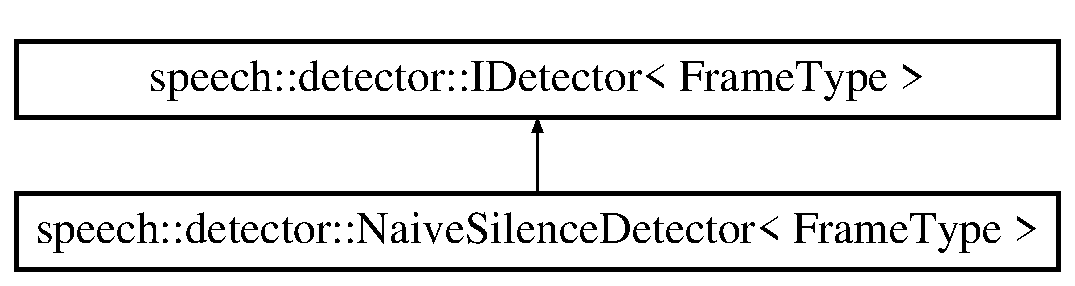
\includegraphics[height=2.000000cm]{classspeech_1_1detector_1_1IDetector}
\end{center}
\end{figure}
\subsection*{Public Member Functions}
\begin{DoxyCompactItemize}
\item 
virtual bool \hyperlink{classspeech_1_1detector_1_1IDetector_a351b24904f920bc42cdcfa1f1c91f479}{detected} (\hyperlink{classspeech_1_1raw__data_1_1FrequencySample}{Frequency\+Sample}$<$ Frame\+Type $>$ \&sample) const =0
\end{DoxyCompactItemize}


\subsection{Member Function Documentation}
\hypertarget{classspeech_1_1detector_1_1IDetector_a351b24904f920bc42cdcfa1f1c91f479}{\index{speech\+::detector\+::\+I\+Detector@{speech\+::detector\+::\+I\+Detector}!detected@{detected}}
\index{detected@{detected}!speech\+::detector\+::\+I\+Detector@{speech\+::detector\+::\+I\+Detector}}
\subsubsection[{detected}]{\setlength{\rightskip}{0pt plus 5cm}template$<$typename Frame\+Type $>$ virtual bool {\bf speech\+::detector\+::\+I\+Detector}$<$ Frame\+Type $>$\+::detected (
\begin{DoxyParamCaption}
\item[{{\bf Frequency\+Sample}$<$ Frame\+Type $>$ \&}]{sample}
\end{DoxyParamCaption}
) const\hspace{0.3cm}{\ttfamily [pure virtual]}}}\label{classspeech_1_1detector_1_1IDetector_a351b24904f920bc42cdcfa1f1c91f479}
Checks the condition of the particular detector, and returns T\+R\+U\+E if the condition was met, F\+A\+L\+S\+E otherwise.

\begin{DoxyReturn}{Returns}
T\+R\+U\+E -\/ if detected the pattern, F\+A\+L\+S\+E otherwise 
\end{DoxyReturn}


Implemented in \hyperlink{classspeech_1_1detector_1_1NaiveSilenceDetector_a5d2bc90b3012c10496b557a96a71aa68}{speech\+::detector\+::\+Naive\+Silence\+Detector$<$ Frame\+Type $>$}.



The documentation for this class was generated from the following file\+:\begin{DoxyCompactItemize}
\item 
/home/kacper/\+Projects/speech-\/recognition/src/speech/detector/I\+Detector.\+h\end{DoxyCompactItemize}

\hypertarget{classspeech_1_1raw__data_1_1filtering_1_1IFrequencySampleFilter}{\section{speech\+:\+:raw\+\_\+data\+:\+:filtering\+:\+:I\+Frequency\+Sample\+Filter$<$ Frame\+Type $>$ Class Template Reference}
\label{classspeech_1_1raw__data_1_1filtering_1_1IFrequencySampleFilter}\index{speech\+::raw\+\_\+data\+::filtering\+::\+I\+Frequency\+Sample\+Filter$<$ Frame\+Type $>$@{speech\+::raw\+\_\+data\+::filtering\+::\+I\+Frequency\+Sample\+Filter$<$ Frame\+Type $>$}}
}
Inheritance diagram for speech\+:\+:raw\+\_\+data\+:\+:filtering\+:\+:I\+Frequency\+Sample\+Filter$<$ Frame\+Type $>$\+:\begin{figure}[H]
\begin{center}
\leavevmode
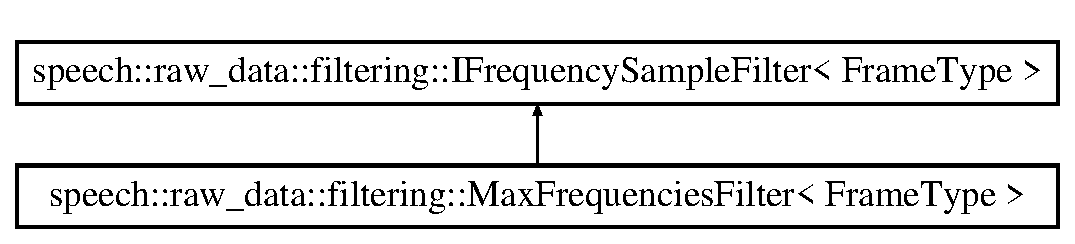
\includegraphics[height=2.000000cm]{classspeech_1_1raw__data_1_1filtering_1_1IFrequencySampleFilter}
\end{center}
\end{figure}
\subsection*{Public Member Functions}
\begin{DoxyCompactItemize}
\item 
\hypertarget{classspeech_1_1raw__data_1_1filtering_1_1IFrequencySampleFilter_a8a6ed0312a73a747f9188dff906ecfd7}{virtual \hyperlink{classspeech_1_1raw__data_1_1FrequencySample}{Frequency\+Sample}\\*
$<$ Frame\+Type $>$ {\bfseries filter} (const \hyperlink{classspeech_1_1raw__data_1_1FrequencySample}{Frequency\+Sample}$<$ Frame\+Type $>$ \&sample)=0}\label{classspeech_1_1raw__data_1_1filtering_1_1IFrequencySampleFilter_a8a6ed0312a73a747f9188dff906ecfd7}

\end{DoxyCompactItemize}


The documentation for this class was generated from the following file\+:\begin{DoxyCompactItemize}
\item 
/home/kacper/\+Projects/speech-\/recognition/src/speech/raw\+\_\+data/filtering/I\+Frequency\+Sample\+Filter.\+h\end{DoxyCompactItemize}

\hypertarget{classspeech_1_1transform_1_1IFrequencyTransform}{\section{speech\+:\+:transform\+:\+:I\+Frequency\+Transform$<$ Frame\+Type $>$ Class Template Reference}
\label{classspeech_1_1transform_1_1IFrequencyTransform}\index{speech\+::transform\+::\+I\+Frequency\+Transform$<$ Frame\+Type $>$@{speech\+::transform\+::\+I\+Frequency\+Transform$<$ Frame\+Type $>$}}
}


{\ttfamily \#include $<$I\+Frequency\+Transform.\+h$>$}

Inheritance diagram for speech\+:\+:transform\+:\+:I\+Frequency\+Transform$<$ Frame\+Type $>$\+:\begin{figure}[H]
\begin{center}
\leavevmode
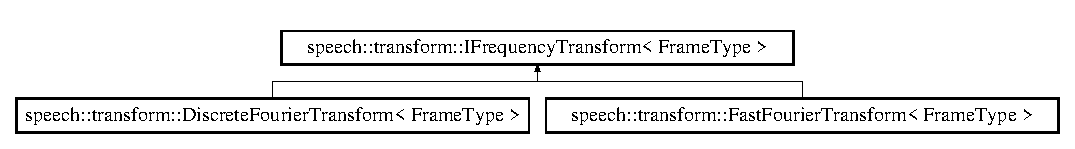
\includegraphics[height=1.555556cm]{classspeech_1_1transform_1_1IFrequencyTransform}
\end{center}
\end{figure}
\subsection*{Public Member Functions}
\begin{DoxyCompactItemize}
\item 
\hypertarget{classspeech_1_1transform_1_1IFrequencyTransform_a2012eb643e7888e08658dccc4f11b206}{virtual \hyperlink{classspeech_1_1raw__data_1_1FrequencySample}{Frequency\+Sample}\\*
$<$ Frame\+Type $>$ {\bfseries transform} (const \hyperlink{classspeech_1_1raw__data_1_1DataSample}{Data\+Sample}$<$ Frame\+Type $>$ \&vector)=0}\label{classspeech_1_1transform_1_1IFrequencyTransform_a2012eb643e7888e08658dccc4f11b206}

\item 
\hypertarget{classspeech_1_1transform_1_1IFrequencyTransform_a2882e1cad03d0a7e6ec373c10ae1ef81}{virtual \hyperlink{classspeech_1_1raw__data_1_1DataSample}{Data\+Sample}$<$ Frame\+Type $>$ {\bfseries reverse\+Transform} (const \hyperlink{classspeech_1_1raw__data_1_1FrequencySample}{Frequency\+Sample}$<$ Frame\+Type $>$ \&vector)=0}\label{classspeech_1_1transform_1_1IFrequencyTransform_a2882e1cad03d0a7e6ec373c10ae1ef81}

\item 
\hypertarget{classspeech_1_1transform_1_1IFrequencyTransform_a3b4f5614232cb3d34c6319304ba93829}{virtual \hyperlink{classspeech_1_1raw__data_1_1FrequencySample}{Frequency\+Sample}\\*
$<$ Frame\+Type $>$ {\bfseries transform} (const \hyperlink{classspeech_1_1raw__data_1_1DataSample}{Data\+Sample}$<$ Frame\+Type $>$ \&vector, \hyperlink{classspeech_1_1transform_1_1window_1_1Window}{Window} $\ast$window)=0}\label{classspeech_1_1transform_1_1IFrequencyTransform_a3b4f5614232cb3d34c6319304ba93829}

\end{DoxyCompactItemize}


\subsection{Detailed Description}
\subsubsection*{template$<$typename Frame\+Type$>$class speech\+::transform\+::\+I\+Frequency\+Transform$<$ Frame\+Type $>$}

This is an interface for all transforms which converts raw signal into frequency domain. 

The documentation for this class was generated from the following file\+:\begin{DoxyCompactItemize}
\item 
/home/kacper/\+Projects/speech-\/recognition/src/speech/transform/I\+Frequency\+Transform.\+h\end{DoxyCompactItemize}

\hypertarget{classspeech_1_1metric_1_1IMetric}{\section{speech\+:\+:metric\+:\+:I\+Metric Class Reference}
\label{classspeech_1_1metric_1_1IMetric}\index{speech\+::metric\+::\+I\+Metric@{speech\+::metric\+::\+I\+Metric}}
}
Inheritance diagram for speech\+:\+:metric\+:\+:I\+Metric\+:\begin{figure}[H]
\begin{center}
\leavevmode
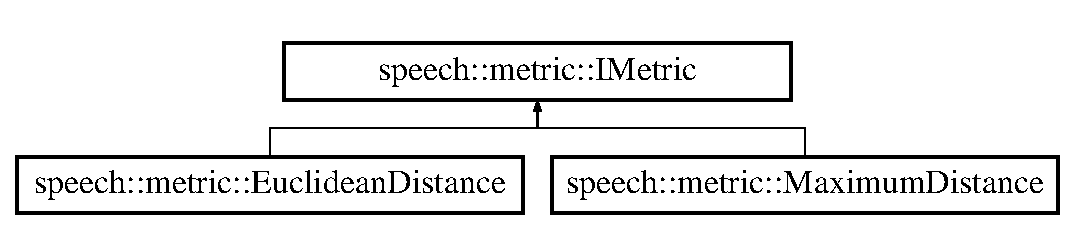
\includegraphics[height=2.000000cm]{classspeech_1_1metric_1_1IMetric}
\end{center}
\end{figure}
\subsection*{Public Member Functions}
\begin{DoxyCompactItemize}
\item 
virtual double \hyperlink{classspeech_1_1metric_1_1IMetric_af15c579c0870b67e862945b6918bc14e}{operator()} (const std\+::valarray$<$ double $>$ \&v1, const std\+::valarray$<$ double $>$ \&v2)=0
\end{DoxyCompactItemize}


\subsection{Member Function Documentation}
\hypertarget{classspeech_1_1metric_1_1IMetric_af15c579c0870b67e862945b6918bc14e}{\index{speech\+::metric\+::\+I\+Metric@{speech\+::metric\+::\+I\+Metric}!operator()@{operator()}}
\index{operator()@{operator()}!speech\+::metric\+::\+I\+Metric@{speech\+::metric\+::\+I\+Metric}}
\subsubsection[{operator()}]{\setlength{\rightskip}{0pt plus 5cm}virtual double speech\+::metric\+::\+I\+Metric\+::operator() (
\begin{DoxyParamCaption}
\item[{const std\+::valarray$<$ double $>$ \&}]{v1, }
\item[{const std\+::valarray$<$ double $>$ \&}]{v2}
\end{DoxyParamCaption}
)\hspace{0.3cm}{\ttfamily [pure virtual]}}}\label{classspeech_1_1metric_1_1IMetric_af15c579c0870b67e862945b6918bc14e}
Calculates a distance between two vectors. \begin{DoxyReturn}{Returns}
a distance 
\end{DoxyReturn}


Implemented in \hyperlink{classspeech_1_1metric_1_1EuclideanDistance_abd0d73ebf83dc218ab8f6ab5dee47064}{speech\+::metric\+::\+Euclidean\+Distance}, and \hyperlink{classspeech_1_1metric_1_1MaximumDistance_aa2c39fc82d79a701aecb8982ac0f2eaf}{speech\+::metric\+::\+Maximum\+Distance}.



The documentation for this class was generated from the following file\+:\begin{DoxyCompactItemize}
\item 
/home/kacper/\+Projects/speech-\/recognition/src/speech/metric/I\+Metric.\+h\end{DoxyCompactItemize}

\hypertarget{classspeech_1_1spelling_1_1ISpellingTranscription}{\section{speech\+:\+:spelling\+:\+:I\+Spelling\+Transcription Class Reference}
\label{classspeech_1_1spelling_1_1ISpellingTranscription}\index{speech\+::spelling\+::\+I\+Spelling\+Transcription@{speech\+::spelling\+::\+I\+Spelling\+Transcription}}
}
Inheritance diagram for speech\+:\+:spelling\+:\+:I\+Spelling\+Transcription\+:\begin{figure}[H]
\begin{center}
\leavevmode
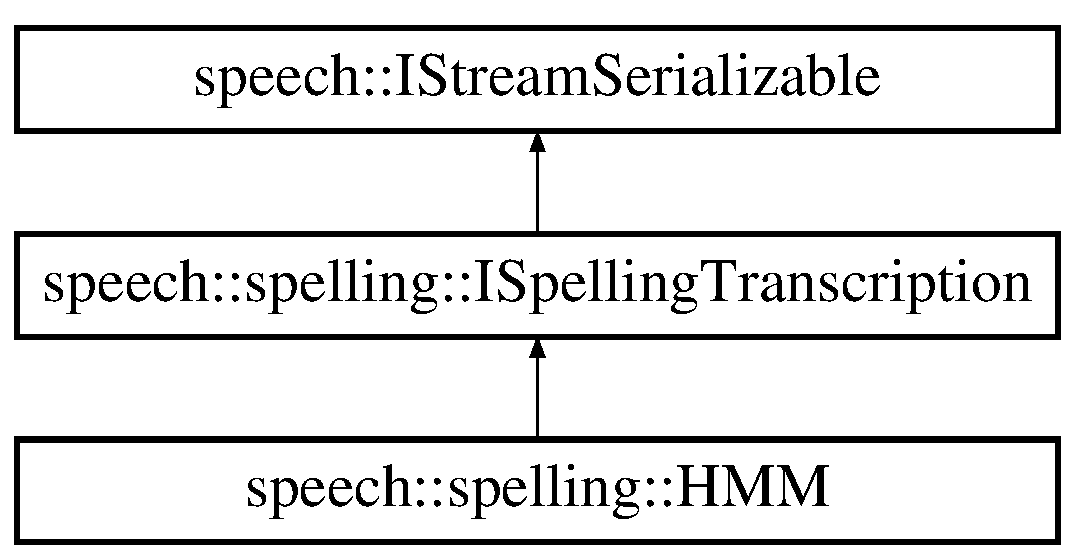
\includegraphics[height=3.000000cm]{classspeech_1_1spelling_1_1ISpellingTranscription}
\end{center}
\end{figure}
\subsection*{Public Member Functions}
\begin{DoxyCompactItemize}
\item 
\hypertarget{classspeech_1_1spelling_1_1ISpellingTranscription_a50dc83bbb65ffb0e37ba6915fbfb43ec}{virtual void {\bfseries fit} (std\+::vector$<$ int $>$ \&phonems, const std\+::string \&spelling)=0}\label{classspeech_1_1spelling_1_1ISpellingTranscription_a50dc83bbb65ffb0e37ba6915fbfb43ec}

\item 
\hypertarget{classspeech_1_1spelling_1_1ISpellingTranscription_a3b3f279e616c29ab102af2b720574e82}{virtual std\+::string {\bfseries predict} (std\+::vector$<$ int $>$ phonems)=0}\label{classspeech_1_1spelling_1_1ISpellingTranscription_a3b3f279e616c29ab102af2b720574e82}

\item 
virtual void \hyperlink{classspeech_1_1spelling_1_1ISpellingTranscription_a2ebd3da352eac002869c2f29ad890b16}{serialize} (std\+::ostream \&out) const =0
\end{DoxyCompactItemize}


\subsection{Member Function Documentation}
\hypertarget{classspeech_1_1spelling_1_1ISpellingTranscription_a2ebd3da352eac002869c2f29ad890b16}{\index{speech\+::spelling\+::\+I\+Spelling\+Transcription@{speech\+::spelling\+::\+I\+Spelling\+Transcription}!serialize@{serialize}}
\index{serialize@{serialize}!speech\+::spelling\+::\+I\+Spelling\+Transcription@{speech\+::spelling\+::\+I\+Spelling\+Transcription}}
\subsubsection[{serialize}]{\setlength{\rightskip}{0pt plus 5cm}virtual void speech\+::spelling\+::\+I\+Spelling\+Transcription\+::serialize (
\begin{DoxyParamCaption}
\item[{std\+::ostream \&}]{out}
\end{DoxyParamCaption}
) const\hspace{0.3cm}{\ttfamily [pure virtual]}}}\label{classspeech_1_1spelling_1_1ISpellingTranscription_a2ebd3da352eac002869c2f29ad890b16}
Writes an object to given stream 
\begin{DoxyParams}{Parameters}
{\em out} & output stream \\
\hline
\end{DoxyParams}


Implements \hyperlink{classspeech_1_1IStreamSerializable_a891561ebe3e4eb5411e613b28bc2c982}{speech\+::\+I\+Stream\+Serializable}.



Implemented in \hyperlink{classspeech_1_1spelling_1_1HMM_a225d39c70f721195c184e8af00ec3651}{speech\+::spelling\+::\+H\+M\+M}.



The documentation for this class was generated from the following file\+:\begin{DoxyCompactItemize}
\item 
/home/kacper/\+Projects/speech-\/recognition/src/speech/spelling/I\+Spelling\+Transcription.\+h\end{DoxyCompactItemize}

\hypertarget{classspeech_1_1IStreamSerializable}{\section{speech\+:\+:I\+Stream\+Serializable Class Reference}
\label{classspeech_1_1IStreamSerializable}\index{speech\+::\+I\+Stream\+Serializable@{speech\+::\+I\+Stream\+Serializable}}
}


{\ttfamily \#include $<$I\+Stream\+Serializable.\+h$>$}

Inheritance diagram for speech\+:\+:I\+Stream\+Serializable\+:\begin{figure}[H]
\begin{center}
\leavevmode
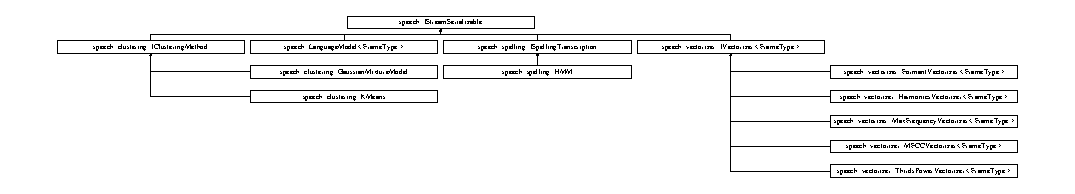
\includegraphics[height=2.165746cm]{classspeech_1_1IStreamSerializable}
\end{center}
\end{figure}
\subsection*{Public Member Functions}
\begin{DoxyCompactItemize}
\item 
virtual void \hyperlink{classspeech_1_1IStreamSerializable_a891561ebe3e4eb5411e613b28bc2c982}{serialize} (std\+::ostream \&out) const =0
\end{DoxyCompactItemize}
\subsection*{Friends}
\begin{DoxyCompactItemize}
\item 
std\+::ostream \& \hyperlink{classspeech_1_1IStreamSerializable_ae1962586a37479716e14c3d8ed3beaca}{operator$<$$<$} (std\+::ostream \&out, const \hyperlink{classspeech_1_1IStreamSerializable}{I\+Stream\+Serializable} \&object)
\end{DoxyCompactItemize}


\subsection{Detailed Description}
This class gives an interface for all classes which can be serialized. All classes used in an language model should inherit from this one, to make sure that it is possible to save the model. 

\subsection{Member Function Documentation}
\hypertarget{classspeech_1_1IStreamSerializable_a891561ebe3e4eb5411e613b28bc2c982}{\index{speech\+::\+I\+Stream\+Serializable@{speech\+::\+I\+Stream\+Serializable}!serialize@{serialize}}
\index{serialize@{serialize}!speech\+::\+I\+Stream\+Serializable@{speech\+::\+I\+Stream\+Serializable}}
\subsubsection[{serialize}]{\setlength{\rightskip}{0pt plus 5cm}virtual void speech\+::\+I\+Stream\+Serializable\+::serialize (
\begin{DoxyParamCaption}
\item[{std\+::ostream \&}]{out}
\end{DoxyParamCaption}
) const\hspace{0.3cm}{\ttfamily [pure virtual]}}}\label{classspeech_1_1IStreamSerializable_a891561ebe3e4eb5411e613b28bc2c982}
Writes an object to given stream 
\begin{DoxyParams}{Parameters}
{\em out} & output stream \\
\hline
\end{DoxyParams}


Implemented in \hyperlink{classspeech_1_1LanguageModel_ae3c30d0a1a1a5e60fd69954b432766fa}{speech\+::\+Language\+Model$<$ Frame\+Type $>$}, \hyperlink{classspeech_1_1vectorizer_1_1MFCCVectorizer_a5f266d0fc3ab4dd89a1d701531818930}{speech\+::vectorizer\+::\+M\+F\+C\+C\+Vectorizer$<$ Frame\+Type $>$}, \hyperlink{classspeech_1_1vectorizer_1_1IVectorizer_aa8285bbd275c31ae1ce48d294400dea9}{speech\+::vectorizer\+::\+I\+Vectorizer$<$ Frame\+Type $>$}, \hyperlink{classspeech_1_1clustering_1_1KMeans_a47ba455f6996f45a1f61cde7e736e254}{speech\+::clustering\+::\+K\+Means}, \hyperlink{classspeech_1_1clustering_1_1GaussianMixtureModel_a51a73a7818e57e5b9e2ff6fbd25188f6}{speech\+::clustering\+::\+Gaussian\+Mixture\+Model}, \hyperlink{classspeech_1_1spelling_1_1HMM_a225d39c70f721195c184e8af00ec3651}{speech\+::spelling\+::\+H\+M\+M}, \hyperlink{classspeech_1_1clustering_1_1IClusteringMethod_a9676e73a7c47d5383e9359850086249c}{speech\+::clustering\+::\+I\+Clustering\+Method}, \hyperlink{classspeech_1_1vectorizer_1_1MaxFrequencyVectorizer_a1fdb7b7544a6386e64e8df49b644a13c}{speech\+::vectorizer\+::\+Max\+Frequency\+Vectorizer$<$ Frame\+Type $>$}, \hyperlink{classspeech_1_1vectorizer_1_1FormantVectorizer_a8eed42b42272eb0d77a49213a5a36f73}{speech\+::vectorizer\+::\+Formant\+Vectorizer$<$ Frame\+Type $>$}, \hyperlink{classspeech_1_1spelling_1_1ISpellingTranscription_a2ebd3da352eac002869c2f29ad890b16}{speech\+::spelling\+::\+I\+Spelling\+Transcription}, \hyperlink{classspeech_1_1vectorizer_1_1HarmonicsVectorizer_a6a9467047e5acbfd0fc4bf1e72679acf}{speech\+::vectorizer\+::\+Harmonics\+Vectorizer$<$ Frame\+Type $>$}, and \hyperlink{classspeech_1_1vectorizer_1_1ThirdsPowerVectorizer_ab27c49171171fa2af908d9f3df0712db}{speech\+::vectorizer\+::\+Thirds\+Power\+Vectorizer$<$ Frame\+Type $>$}.



\subsection{Friends And Related Function Documentation}
\hypertarget{classspeech_1_1IStreamSerializable_ae1962586a37479716e14c3d8ed3beaca}{\index{speech\+::\+I\+Stream\+Serializable@{speech\+::\+I\+Stream\+Serializable}!operator$<$$<$@{operator$<$$<$}}
\index{operator$<$$<$@{operator$<$$<$}!speech\+::\+I\+Stream\+Serializable@{speech\+::\+I\+Stream\+Serializable}}
\subsubsection[{operator$<$$<$}]{\setlength{\rightskip}{0pt plus 5cm}std\+::ostream\& operator$<$$<$ (
\begin{DoxyParamCaption}
\item[{std\+::ostream \&}]{out, }
\item[{const {\bf I\+Stream\+Serializable} \&}]{object}
\end{DoxyParamCaption}
)\hspace{0.3cm}{\ttfamily [friend]}}}\label{classspeech_1_1IStreamSerializable_ae1962586a37479716e14c3d8ed3beaca}
Overloads stream $<$$<$ operator, to allow passing instances of \hyperlink{classspeech_1_1IStreamSerializable}{I\+Stream\+Serializable} into streams; 

The documentation for this class was generated from the following file\+:\begin{DoxyCompactItemize}
\item 
/home/kacper/\+Projects/speech-\/recognition/src/speech/I\+Stream\+Serializable.\+h\end{DoxyCompactItemize}

\hypertarget{classspeech_1_1vectorizer_1_1IVectorizer}{\section{speech\+:\+:vectorizer\+:\+:I\+Vectorizer$<$ Frame\+Type $>$ Class Template Reference}
\label{classspeech_1_1vectorizer_1_1IVectorizer}\index{speech\+::vectorizer\+::\+I\+Vectorizer$<$ Frame\+Type $>$@{speech\+::vectorizer\+::\+I\+Vectorizer$<$ Frame\+Type $>$}}
}
Inheritance diagram for speech\+:\+:vectorizer\+:\+:I\+Vectorizer$<$ Frame\+Type $>$\+:\begin{figure}[H]
\begin{center}
\leavevmode
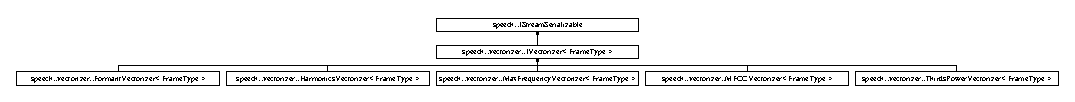
\includegraphics[height=0.928177cm]{classspeech_1_1vectorizer_1_1IVectorizer}
\end{center}
\end{figure}
\subsection*{Public Member Functions}
\begin{DoxyCompactItemize}
\item 
virtual std\+::valarray$<$ double $>$ \hyperlink{classspeech_1_1vectorizer_1_1IVectorizer_a00d2ba71ec5c447780ffb0a29bfc9085}{vectorize} (\hyperlink{classspeech_1_1raw__data_1_1FrequencySample}{Frequency\+Sample}$<$ Frame\+Type $>$ \&sample)=0
\item 
virtual std\+::vector\\*
$<$ std\+::valarray$<$ double $>$ $>$ \hyperlink{classspeech_1_1vectorizer_1_1IVectorizer_a63f089697df0617f89e762582e0daef5}{vectorize} (std\+::vector$<$ \hyperlink{classspeech_1_1raw__data_1_1FrequencySample}{Frequency\+Sample}$<$ Frame\+Type $>$$>$ \&samples)
\item 
virtual std\+::vector\\*
$<$ std\+::valarray$<$ double $>$ $>$ \hyperlink{classspeech_1_1vectorizer_1_1IVectorizer_a2607a7ea800c639136c0ffb38f6aece4}{vectorize} (\hyperlink{classspeech_1_1raw__data_1_1DataSource}{Data\+Source}$<$ Frame\+Type $>$ \&data\+Source)
\item 
virtual void \hyperlink{classspeech_1_1vectorizer_1_1IVectorizer_aa8285bbd275c31ae1ce48d294400dea9}{serialize} (std\+::ostream \&out) const =0
\item 
virtual int \hyperlink{classspeech_1_1vectorizer_1_1IVectorizer_abe20529a1586c072783f42476ad7ab69}{get\+Vector\+Size} () const =0
\end{DoxyCompactItemize}
\subsection*{Protected Attributes}
\begin{DoxyCompactItemize}
\item 
\hyperlink{classspeech_1_1transform_1_1IFrequencyTransform}{I\+Frequency\+Transform}$<$ Frame\+Type $>$ $\ast$ \hyperlink{classspeech_1_1vectorizer_1_1IVectorizer_a947ba92d26dafe78b184410c8db083a5}{frequency\+Transform} = new \hyperlink{classspeech_1_1transform_1_1FastFourierTransform}{Fast\+Fourier\+Transform}$<$Frame\+Type$>$()
\end{DoxyCompactItemize}


\subsection{Member Function Documentation}
\hypertarget{classspeech_1_1vectorizer_1_1IVectorizer_abe20529a1586c072783f42476ad7ab69}{\index{speech\+::vectorizer\+::\+I\+Vectorizer@{speech\+::vectorizer\+::\+I\+Vectorizer}!get\+Vector\+Size@{get\+Vector\+Size}}
\index{get\+Vector\+Size@{get\+Vector\+Size}!speech\+::vectorizer\+::\+I\+Vectorizer@{speech\+::vectorizer\+::\+I\+Vectorizer}}
\subsubsection[{get\+Vector\+Size}]{\setlength{\rightskip}{0pt plus 5cm}template$<$typename Frame\+Type $>$ virtual int {\bf speech\+::vectorizer\+::\+I\+Vectorizer}$<$ Frame\+Type $>$\+::get\+Vector\+Size (
\begin{DoxyParamCaption}
{}
\end{DoxyParamCaption}
) const\hspace{0.3cm}{\ttfamily [pure virtual]}}}\label{classspeech_1_1vectorizer_1_1IVectorizer_abe20529a1586c072783f42476ad7ab69}
Gets the size of the output vector produced by the vectorizer.

\begin{DoxyReturn}{Returns}
size of the produced vector 
\end{DoxyReturn}


Implemented in \hyperlink{classspeech_1_1vectorizer_1_1MFCCVectorizer_a47475baa543b7fe77f227d1e0288b99d}{speech\+::vectorizer\+::\+M\+F\+C\+C\+Vectorizer$<$ Frame\+Type $>$}, \hyperlink{classspeech_1_1vectorizer_1_1MaxFrequencyVectorizer_af92f2750d71a14cbc74d8508f8dbb354}{speech\+::vectorizer\+::\+Max\+Frequency\+Vectorizer$<$ Frame\+Type $>$}, \hyperlink{classspeech_1_1vectorizer_1_1FormantVectorizer_a50b6e8aeace5dab5f7365b57477b7333}{speech\+::vectorizer\+::\+Formant\+Vectorizer$<$ Frame\+Type $>$}, \hyperlink{classspeech_1_1vectorizer_1_1HarmonicsVectorizer_aa6c06fb4864a9bd9e67675b6d836170f}{speech\+::vectorizer\+::\+Harmonics\+Vectorizer$<$ Frame\+Type $>$}, and \hyperlink{classspeech_1_1vectorizer_1_1ThirdsPowerVectorizer_a4680e178d5ef376cf2e4f6d47487e047}{speech\+::vectorizer\+::\+Thirds\+Power\+Vectorizer$<$ Frame\+Type $>$}.

\hypertarget{classspeech_1_1vectorizer_1_1IVectorizer_aa8285bbd275c31ae1ce48d294400dea9}{\index{speech\+::vectorizer\+::\+I\+Vectorizer@{speech\+::vectorizer\+::\+I\+Vectorizer}!serialize@{serialize}}
\index{serialize@{serialize}!speech\+::vectorizer\+::\+I\+Vectorizer@{speech\+::vectorizer\+::\+I\+Vectorizer}}
\subsubsection[{serialize}]{\setlength{\rightskip}{0pt plus 5cm}template$<$typename Frame\+Type $>$ virtual void {\bf speech\+::vectorizer\+::\+I\+Vectorizer}$<$ Frame\+Type $>$\+::serialize (
\begin{DoxyParamCaption}
\item[{std\+::ostream \&}]{out}
\end{DoxyParamCaption}
) const\hspace{0.3cm}{\ttfamily [pure virtual]}}}\label{classspeech_1_1vectorizer_1_1IVectorizer_aa8285bbd275c31ae1ce48d294400dea9}
Serializes the vectorizer into given stream. 
\begin{DoxyParams}{Parameters}
{\em out} & output stream \\
\hline
\end{DoxyParams}


Implements \hyperlink{classspeech_1_1IStreamSerializable_a891561ebe3e4eb5411e613b28bc2c982}{speech\+::\+I\+Stream\+Serializable}.



Implemented in \hyperlink{classspeech_1_1vectorizer_1_1MFCCVectorizer_a5f266d0fc3ab4dd89a1d701531818930}{speech\+::vectorizer\+::\+M\+F\+C\+C\+Vectorizer$<$ Frame\+Type $>$}, \hyperlink{classspeech_1_1vectorizer_1_1MaxFrequencyVectorizer_a1fdb7b7544a6386e64e8df49b644a13c}{speech\+::vectorizer\+::\+Max\+Frequency\+Vectorizer$<$ Frame\+Type $>$}, \hyperlink{classspeech_1_1vectorizer_1_1FormantVectorizer_a8eed42b42272eb0d77a49213a5a36f73}{speech\+::vectorizer\+::\+Formant\+Vectorizer$<$ Frame\+Type $>$}, \hyperlink{classspeech_1_1vectorizer_1_1HarmonicsVectorizer_a6a9467047e5acbfd0fc4bf1e72679acf}{speech\+::vectorizer\+::\+Harmonics\+Vectorizer$<$ Frame\+Type $>$}, and \hyperlink{classspeech_1_1vectorizer_1_1ThirdsPowerVectorizer_ab27c49171171fa2af908d9f3df0712db}{speech\+::vectorizer\+::\+Thirds\+Power\+Vectorizer$<$ Frame\+Type $>$}.

\hypertarget{classspeech_1_1vectorizer_1_1IVectorizer_a00d2ba71ec5c447780ffb0a29bfc9085}{\index{speech\+::vectorizer\+::\+I\+Vectorizer@{speech\+::vectorizer\+::\+I\+Vectorizer}!vectorize@{vectorize}}
\index{vectorize@{vectorize}!speech\+::vectorizer\+::\+I\+Vectorizer@{speech\+::vectorizer\+::\+I\+Vectorizer}}
\subsubsection[{vectorize}]{\setlength{\rightskip}{0pt plus 5cm}template$<$typename Frame\+Type $>$ virtual std\+::valarray$<$double$>$ {\bf speech\+::vectorizer\+::\+I\+Vectorizer}$<$ Frame\+Type $>$\+::vectorize (
\begin{DoxyParamCaption}
\item[{{\bf Frequency\+Sample}$<$ Frame\+Type $>$ \&}]{sample}
\end{DoxyParamCaption}
)\hspace{0.3cm}{\ttfamily [pure virtual]}}}\label{classspeech_1_1vectorizer_1_1IVectorizer_a00d2ba71ec5c447780ffb0a29bfc9085}
Projects given sample into feature space. Each vector needs to have exactly same size. 
\begin{DoxyParams}{Parameters}
{\em sample} & single sample to be vectorized\\
\hline
\end{DoxyParams}
\begin{DoxyReturn}{Returns}
the projection of vector in a feature space 
\end{DoxyReturn}


Implemented in \hyperlink{classspeech_1_1vectorizer_1_1MFCCVectorizer_ad494d113915e9a5d0bbecda045cf8799}{speech\+::vectorizer\+::\+M\+F\+C\+C\+Vectorizer$<$ Frame\+Type $>$}, \hyperlink{classspeech_1_1vectorizer_1_1MaxFrequencyVectorizer_a9463cc7d335fdc5d181d2dffbd488a12}{speech\+::vectorizer\+::\+Max\+Frequency\+Vectorizer$<$ Frame\+Type $>$}, \hyperlink{classspeech_1_1vectorizer_1_1FormantVectorizer_a80e578bcd5f23d4b9237589669e20a1a}{speech\+::vectorizer\+::\+Formant\+Vectorizer$<$ Frame\+Type $>$}, \hyperlink{classspeech_1_1vectorizer_1_1HarmonicsVectorizer_a7f2d8f5d43c416ae95025d63c54d4385}{speech\+::vectorizer\+::\+Harmonics\+Vectorizer$<$ Frame\+Type $>$}, and \hyperlink{classspeech_1_1vectorizer_1_1ThirdsPowerVectorizer_aa43af654f25abdb9a1698815edaf900c}{speech\+::vectorizer\+::\+Thirds\+Power\+Vectorizer$<$ Frame\+Type $>$}.

\hypertarget{classspeech_1_1vectorizer_1_1IVectorizer_a63f089697df0617f89e762582e0daef5}{\index{speech\+::vectorizer\+::\+I\+Vectorizer@{speech\+::vectorizer\+::\+I\+Vectorizer}!vectorize@{vectorize}}
\index{vectorize@{vectorize}!speech\+::vectorizer\+::\+I\+Vectorizer@{speech\+::vectorizer\+::\+I\+Vectorizer}}
\subsubsection[{vectorize}]{\setlength{\rightskip}{0pt plus 5cm}template$<$typename Frame\+Type $>$ virtual std\+::vector$<$std\+::valarray$<$double$>$ $>$ {\bf speech\+::vectorizer\+::\+I\+Vectorizer}$<$ Frame\+Type $>$\+::vectorize (
\begin{DoxyParamCaption}
\item[{std\+::vector$<$ {\bf Frequency\+Sample}$<$ Frame\+Type $>$$>$ \&}]{samples}
\end{DoxyParamCaption}
)\hspace{0.3cm}{\ttfamily [inline]}, {\ttfamily [virtual]}}}\label{classspeech_1_1vectorizer_1_1IVectorizer_a63f089697df0617f89e762582e0daef5}
Projects all samples from given collection into feature space. Each vector needs to have the same dimension. 
\begin{DoxyParams}{Parameters}
{\em samples} & a collection of frequency domain samples \\
\hline
\end{DoxyParams}
\begin{DoxyRefDesc}{Deprecated}
\item[\hyperlink{deprecated__deprecated000001}{Deprecated}]pass the data source instead \begin{DoxyReturn}{Returns}
the projection of all vectors from given collection 
\end{DoxyReturn}
\end{DoxyRefDesc}


Reimplemented in \hyperlink{classspeech_1_1vectorizer_1_1MFCCVectorizer_a21a1862ff866a77c540943f48a6511d2}{speech\+::vectorizer\+::\+M\+F\+C\+C\+Vectorizer$<$ Frame\+Type $>$}.

\hypertarget{classspeech_1_1vectorizer_1_1IVectorizer_a2607a7ea800c639136c0ffb38f6aece4}{\index{speech\+::vectorizer\+::\+I\+Vectorizer@{speech\+::vectorizer\+::\+I\+Vectorizer}!vectorize@{vectorize}}
\index{vectorize@{vectorize}!speech\+::vectorizer\+::\+I\+Vectorizer@{speech\+::vectorizer\+::\+I\+Vectorizer}}
\subsubsection[{vectorize}]{\setlength{\rightskip}{0pt plus 5cm}template$<$typename Frame\+Type $>$ virtual std\+::vector$<$std\+::valarray$<$double$>$ $>$ {\bf speech\+::vectorizer\+::\+I\+Vectorizer}$<$ Frame\+Type $>$\+::vectorize (
\begin{DoxyParamCaption}
\item[{{\bf Data\+Source}$<$ Frame\+Type $>$ \&}]{data\+Source}
\end{DoxyParamCaption}
)\hspace{0.3cm}{\ttfamily [inline]}, {\ttfamily [virtual]}}}\label{classspeech_1_1vectorizer_1_1IVectorizer_a2607a7ea800c639136c0ffb38f6aece4}
Projects all samples from given data source into feature space. 
\begin{DoxyParams}{Parameters}
{\em data\+Source} & data source containing the samples\\
\hline
\end{DoxyParams}
\begin{DoxyReturn}{Returns}
collection of all vectorized samples 
\end{DoxyReturn}


Reimplemented in \hyperlink{classspeech_1_1vectorizer_1_1MFCCVectorizer_a7faab008b85e4fd817a04194b6470e88}{speech\+::vectorizer\+::\+M\+F\+C\+C\+Vectorizer$<$ Frame\+Type $>$}.



\subsection{Member Data Documentation}
\hypertarget{classspeech_1_1vectorizer_1_1IVectorizer_a947ba92d26dafe78b184410c8db083a5}{\index{speech\+::vectorizer\+::\+I\+Vectorizer@{speech\+::vectorizer\+::\+I\+Vectorizer}!frequency\+Transform@{frequency\+Transform}}
\index{frequency\+Transform@{frequency\+Transform}!speech\+::vectorizer\+::\+I\+Vectorizer@{speech\+::vectorizer\+::\+I\+Vectorizer}}
\subsubsection[{frequency\+Transform}]{\setlength{\rightskip}{0pt plus 5cm}template$<$typename Frame\+Type $>$ {\bf I\+Frequency\+Transform}$<$Frame\+Type$>$$\ast$ {\bf speech\+::vectorizer\+::\+I\+Vectorizer}$<$ Frame\+Type $>$\+::frequency\+Transform = new {\bf Fast\+Fourier\+Transform}$<$Frame\+Type$>$()\hspace{0.3cm}{\ttfamily [protected]}}}\label{classspeech_1_1vectorizer_1_1IVectorizer_a947ba92d26dafe78b184410c8db083a5}
Transform between time and frequency domain 

The documentation for this class was generated from the following file\+:\begin{DoxyCompactItemize}
\item 
/home/kacper/\+Projects/speech-\/recognition/src/speech/vectorizer/I\+Vectorizer.\+h\end{DoxyCompactItemize}

\hypertarget{classspeech_1_1clustering_1_1KMeans}{\section{speech\+:\+:clustering\+:\+:K\+Means Class Reference}
\label{classspeech_1_1clustering_1_1KMeans}\index{speech\+::clustering\+::\+K\+Means@{speech\+::clustering\+::\+K\+Means}}
}


{\ttfamily \#include $<$K\+Means.\+h$>$}

Inheritance diagram for speech\+:\+:clustering\+:\+:K\+Means\+:\begin{figure}[H]
\begin{center}
\leavevmode
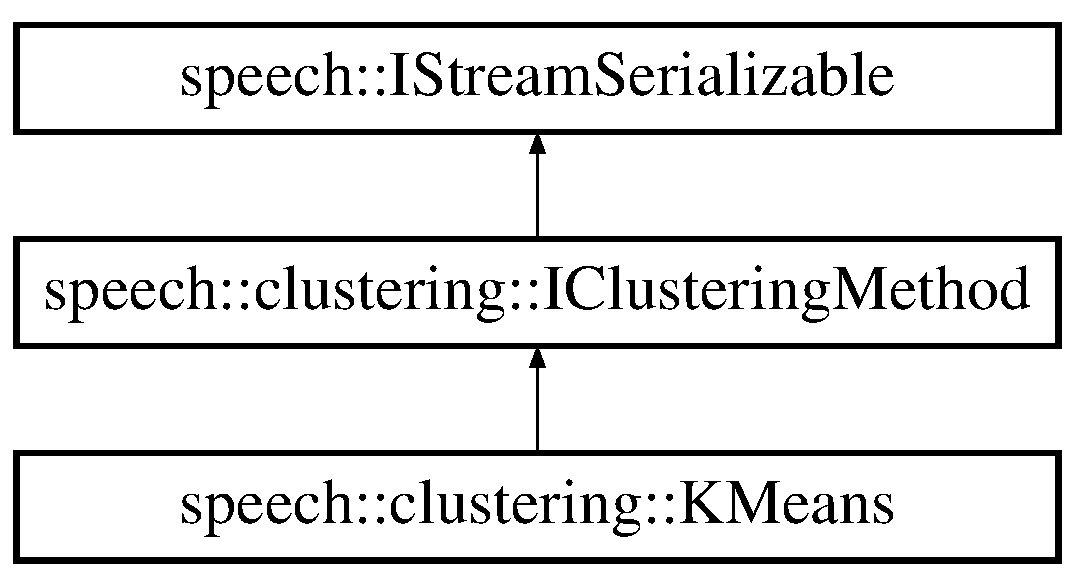
\includegraphics[height=3.000000cm]{classspeech_1_1clustering_1_1KMeans}
\end{center}
\end{figure}
\subsection*{Public Member Functions}
\begin{DoxyCompactItemize}
\item 
\hyperlink{classspeech_1_1clustering_1_1KMeans_a24b819b6569e1b2228d4ff1b7a8dde40}{K\+Means} (std\+::istream \&in)
\item 
\hyperlink{classspeech_1_1clustering_1_1KMeans_a22d1f19adeed74ce6452aec02addd1ae}{K\+Means} (unsigned int \+\_\+k, unsigned int \+\_\+dim)
\item 
virtual \hyperlink{classspeech_1_1clustering_1_1KMeans_aaac97c4e9820cb0f3525b4a13a73ad30}{$\sim$\+K\+Means} ()
\item 
virtual void \hyperlink{classspeech_1_1clustering_1_1KMeans_a53a00478141ceee40366602a85e31ff4}{fit} (vector$<$ valarray$<$ double $>$$>$ \&vectors)
\item 
virtual int \hyperlink{classspeech_1_1clustering_1_1KMeans_a6b87bc8e097b0933220b7083ec846325}{predict} (const valarray$<$ double $>$ \&vector)
\item 
\hypertarget{classspeech_1_1clustering_1_1KMeans_a31e5171317f951f8138ff39b920b8807}{std\+::vector$<$ std\+::valarray\\*
$<$ double $>$ $>$ $\ast$ {\bfseries get\+Centroids} () const }\label{classspeech_1_1clustering_1_1KMeans_a31e5171317f951f8138ff39b920b8807}

\item 
virtual void \hyperlink{classspeech_1_1clustering_1_1KMeans_a47ba455f6996f45a1f61cde7e736e254}{serialize} (std\+::ostream \&out) const 
\end{DoxyCompactItemize}
\subsection*{Public Attributes}
\begin{DoxyCompactItemize}
\item 
\hypertarget{classspeech_1_1clustering_1_1KMeans_a23ff9ad53e6d3db5d933ca6369d36ebe}{const unsigned int {\bfseries M\+A\+X\+\_\+\+I\+T\+E\+R\+A\+T\+I\+O\+N\+S} = 100000}\label{classspeech_1_1clustering_1_1KMeans_a23ff9ad53e6d3db5d933ca6369d36ebe}

\item 
\hypertarget{classspeech_1_1clustering_1_1KMeans_a51592e6258feb92faf71ed61a083596a}{const double {\bfseries E\+P\+S} = 10e-\/64}\label{classspeech_1_1clustering_1_1KMeans_a51592e6258feb92faf71ed61a083596a}

\end{DoxyCompactItemize}
\subsection*{Static Public Attributes}
\begin{DoxyCompactItemize}
\item 
\hypertarget{classspeech_1_1clustering_1_1KMeans_a2643066179760a8455dc118e860a9c5d}{static const uint32\+\_\+t {\bfseries T\+Y\+P\+E\+\_\+\+I\+D\+E\+N\+T\+I\+F\+I\+E\+R} = 0x00000001}\label{classspeech_1_1clustering_1_1KMeans_a2643066179760a8455dc118e860a9c5d}

\end{DoxyCompactItemize}


\subsection{Detailed Description}
This is an implementation of \hyperlink{classspeech_1_1clustering_1_1KMeans}{K\+Means} algorithm. \begin{DoxySeeAlso}{See also}
\href{http://en.wikipedia.org/wiki/K-means_clustering}{\tt http\+://en.\+wikipedia.\+org/wiki/\+K-\/means\+\_\+clustering} 
\end{DoxySeeAlso}


\subsection{Constructor \& Destructor Documentation}
\hypertarget{classspeech_1_1clustering_1_1KMeans_a24b819b6569e1b2228d4ff1b7a8dde40}{\index{speech\+::clustering\+::\+K\+Means@{speech\+::clustering\+::\+K\+Means}!K\+Means@{K\+Means}}
\index{K\+Means@{K\+Means}!speech\+::clustering\+::\+K\+Means@{speech\+::clustering\+::\+K\+Means}}
\subsubsection[{K\+Means}]{\setlength{\rightskip}{0pt plus 5cm}speech\+::clustering\+::\+K\+Means\+::\+K\+Means (
\begin{DoxyParamCaption}
\item[{std\+::istream \&}]{in}
\end{DoxyParamCaption}
)}}\label{classspeech_1_1clustering_1_1KMeans_a24b819b6569e1b2228d4ff1b7a8dde40}
Construct a clustering method from a stream. 
\begin{DoxyParams}{Parameters}
{\em in} & stream containing serialized model \\
\hline
\end{DoxyParams}
\hypertarget{classspeech_1_1clustering_1_1KMeans_a22d1f19adeed74ce6452aec02addd1ae}{\index{speech\+::clustering\+::\+K\+Means@{speech\+::clustering\+::\+K\+Means}!K\+Means@{K\+Means}}
\index{K\+Means@{K\+Means}!speech\+::clustering\+::\+K\+Means@{speech\+::clustering\+::\+K\+Means}}
\subsubsection[{K\+Means}]{\setlength{\rightskip}{0pt plus 5cm}speech\+::clustering\+::\+K\+Means\+::\+K\+Means (
\begin{DoxyParamCaption}
\item[{unsigned int}]{\+\_\+k, }
\item[{unsigned int}]{\+\_\+dim}
\end{DoxyParamCaption}
)}}\label{classspeech_1_1clustering_1_1KMeans_a22d1f19adeed74ce6452aec02addd1ae}
Construct a clustering method with given parameters. 
\begin{DoxyParams}{Parameters}
{\em \+\_\+k} & number of clusters \\
\hline
{\em \+\_\+dim} & dimension of a single vector \\
\hline
\end{DoxyParams}
\hypertarget{classspeech_1_1clustering_1_1KMeans_aaac97c4e9820cb0f3525b4a13a73ad30}{\index{speech\+::clustering\+::\+K\+Means@{speech\+::clustering\+::\+K\+Means}!````~K\+Means@{$\sim$\+K\+Means}}
\index{````~K\+Means@{$\sim$\+K\+Means}!speech\+::clustering\+::\+K\+Means@{speech\+::clustering\+::\+K\+Means}}
\subsubsection[{$\sim$\+K\+Means}]{\setlength{\rightskip}{0pt plus 5cm}speech\+::clustering\+::\+K\+Means\+::$\sim$\+K\+Means (
\begin{DoxyParamCaption}
{}
\end{DoxyParamCaption}
)\hspace{0.3cm}{\ttfamily [virtual]}}}\label{classspeech_1_1clustering_1_1KMeans_aaac97c4e9820cb0f3525b4a13a73ad30}
Destructor 

\subsection{Member Function Documentation}
\hypertarget{classspeech_1_1clustering_1_1KMeans_a53a00478141ceee40366602a85e31ff4}{\index{speech\+::clustering\+::\+K\+Means@{speech\+::clustering\+::\+K\+Means}!fit@{fit}}
\index{fit@{fit}!speech\+::clustering\+::\+K\+Means@{speech\+::clustering\+::\+K\+Means}}
\subsubsection[{fit}]{\setlength{\rightskip}{0pt plus 5cm}void speech\+::clustering\+::\+K\+Means\+::fit (
\begin{DoxyParamCaption}
\item[{vector$<$ valarray$<$ double $>$$>$ \&}]{vectors}
\end{DoxyParamCaption}
)\hspace{0.3cm}{\ttfamily [virtual]}}}\label{classspeech_1_1clustering_1_1KMeans_a53a00478141ceee40366602a85e31ff4}
Fit the \hyperlink{classspeech_1_1clustering_1_1KMeans}{K\+Means} model using standard algorithm\+:
\begin{DoxyEnumerate}
\item Randomly choose k centroids from given vectors' set
\item In each iteration assign all vectors into the nearest centroid
\item Update each centroid to be a mean of the all vectors belonging to this particular group
\item Stop when nothing changed in an iteration or after maximum number of iterations 
\end{DoxyEnumerate}

Implements \hyperlink{classspeech_1_1clustering_1_1IClusteringMethod_ab9ec001a1f76be4793086cd8548ac886}{speech\+::clustering\+::\+I\+Clustering\+Method}.

\hypertarget{classspeech_1_1clustering_1_1KMeans_a6b87bc8e097b0933220b7083ec846325}{\index{speech\+::clustering\+::\+K\+Means@{speech\+::clustering\+::\+K\+Means}!predict@{predict}}
\index{predict@{predict}!speech\+::clustering\+::\+K\+Means@{speech\+::clustering\+::\+K\+Means}}
\subsubsection[{predict}]{\setlength{\rightskip}{0pt plus 5cm}int speech\+::clustering\+::\+K\+Means\+::predict (
\begin{DoxyParamCaption}
\item[{const valarray$<$ double $>$ \&}]{vector}
\end{DoxyParamCaption}
)\hspace{0.3cm}{\ttfamily [virtual]}}}\label{classspeech_1_1clustering_1_1KMeans_a6b87bc8e097b0933220b7083ec846325}
Select the most probable label for the given vector. Label is a position of the closest centroid.

\begin{DoxyReturn}{Returns}
predicted label 
\end{DoxyReturn}


Implements \hyperlink{classspeech_1_1clustering_1_1IClusteringMethod_a47be2ed9fbe6792dcebc8fdcee7fa76e}{speech\+::clustering\+::\+I\+Clustering\+Method}.

\hypertarget{classspeech_1_1clustering_1_1KMeans_a47ba455f6996f45a1f61cde7e736e254}{\index{speech\+::clustering\+::\+K\+Means@{speech\+::clustering\+::\+K\+Means}!serialize@{serialize}}
\index{serialize@{serialize}!speech\+::clustering\+::\+K\+Means@{speech\+::clustering\+::\+K\+Means}}
\subsubsection[{serialize}]{\setlength{\rightskip}{0pt plus 5cm}void speech\+::clustering\+::\+K\+Means\+::serialize (
\begin{DoxyParamCaption}
\item[{std\+::ostream \&}]{out}
\end{DoxyParamCaption}
) const\hspace{0.3cm}{\ttfamily [virtual]}}}\label{classspeech_1_1clustering_1_1KMeans_a47ba455f6996f45a1f61cde7e736e254}
Serialize a model into given stream. 
\begin{DoxyParams}{Parameters}
{\em out} & stream to serialize the model into \\
\hline
\end{DoxyParams}


Implements \hyperlink{classspeech_1_1clustering_1_1IClusteringMethod_a9676e73a7c47d5383e9359850086249c}{speech\+::clustering\+::\+I\+Clustering\+Method}.



The documentation for this class was generated from the following files\+:\begin{DoxyCompactItemize}
\item 
/home/kacper/\+Projects/speech-\/recognition/src/speech/clustering/K\+Means.\+h\item 
/home/kacper/\+Projects/speech-\/recognition/src/speech/clustering/K\+Means.\+cpp\end{DoxyCompactItemize}

\hypertarget{classspeech_1_1initializer_1_1KMeansInitializer}{\section{speech\+:\+:initializer\+:\+:K\+Means\+Initializer Class Reference}
\label{classspeech_1_1initializer_1_1KMeansInitializer}\index{speech\+::initializer\+::\+K\+Means\+Initializer@{speech\+::initializer\+::\+K\+Means\+Initializer}}
}


{\ttfamily \#include $<$K\+Means\+Initializer.\+h$>$}

Inheritance diagram for speech\+:\+:initializer\+:\+:K\+Means\+Initializer\+:\begin{figure}[H]
\begin{center}
\leavevmode
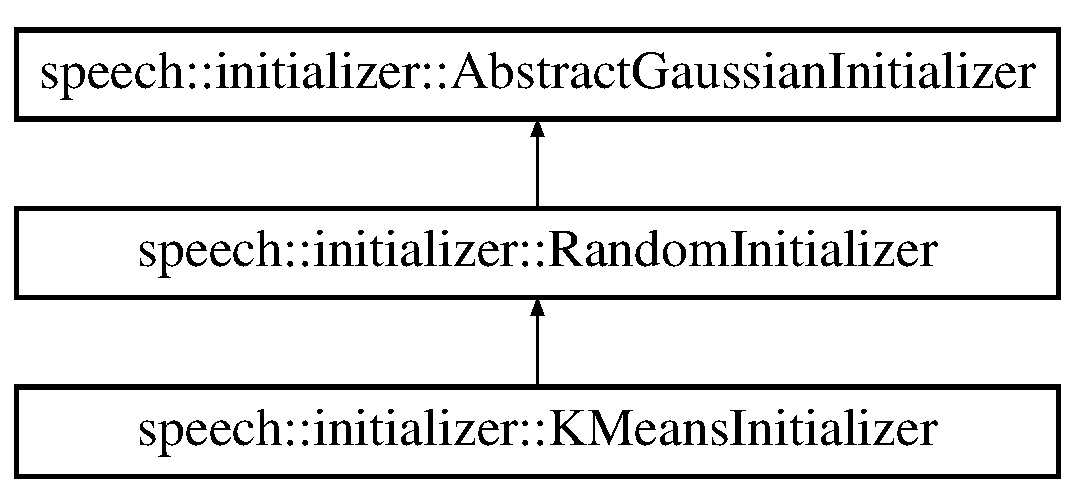
\includegraphics[height=3.000000cm]{classspeech_1_1initializer_1_1KMeansInitializer}
\end{center}
\end{figure}
\subsection*{Public Member Functions}
\begin{DoxyCompactItemize}
\item 
virtual void \hyperlink{classspeech_1_1initializer_1_1KMeansInitializer_a300e51ef3bca3d566bffb12f2c6f5924}{initialize} (\hyperlink{classspeech_1_1HMMLexicon_1_1MultivariateGaussianHMM}{speech\+::\+H\+M\+M\+Lexicon\+::\+Multivariate\+Gaussian\+H\+M\+M} \&gaussian\+H\+M\+M)
\end{DoxyCompactItemize}
\subsection*{Additional Inherited Members}


\subsection{Detailed Description}
Initializer choosing initial estimates using K\+Means clustering 

\subsection{Member Function Documentation}
\hypertarget{classspeech_1_1initializer_1_1KMeansInitializer_a300e51ef3bca3d566bffb12f2c6f5924}{\index{speech\+::initializer\+::\+K\+Means\+Initializer@{speech\+::initializer\+::\+K\+Means\+Initializer}!initialize@{initialize}}
\index{initialize@{initialize}!speech\+::initializer\+::\+K\+Means\+Initializer@{speech\+::initializer\+::\+K\+Means\+Initializer}}
\subsubsection[{initialize}]{\setlength{\rightskip}{0pt plus 5cm}void speech\+::initializer\+::\+K\+Means\+Initializer\+::initialize (
\begin{DoxyParamCaption}
\item[{{\bf speech\+::\+H\+M\+M\+Lexicon\+::\+Multivariate\+Gaussian\+H\+M\+M} \&}]{gaussian\+H\+M\+M}
\end{DoxyParamCaption}
)\hspace{0.3cm}{\ttfamily [virtual]}}}\label{classspeech_1_1initializer_1_1KMeansInitializer_a300e51ef3bca3d566bffb12f2c6f5924}
Initializes the Gaussians of given H\+M\+M with means and variances 
\begin{DoxyParams}{Parameters}
{\em gaussian\+Hmm} & instance of Gaussian H\+M\+M \\
\hline
\end{DoxyParams}


Reimplemented from \hyperlink{classspeech_1_1initializer_1_1RandomInitializer_a62c031971e30c4c99516a20268511963}{speech\+::initializer\+::\+Random\+Initializer}.



The documentation for this class was generated from the following files\+:\begin{DoxyCompactItemize}
\item 
/home/kacper/\+Projects/speech-\/recognition/src/speech/initializer/K\+Means\+Initializer.\+h\item 
/home/kacper/\+Projects/speech-\/recognition/src/speech/initializer/K\+Means\+Initializer.\+cpp\end{DoxyCompactItemize}

\hypertarget{classspeech_1_1LanguageModel}{\section{speech\+:\+:Language\+Model$<$ Frame\+Type $>$ Class Template Reference}
\label{classspeech_1_1LanguageModel}\index{speech\+::\+Language\+Model$<$ Frame\+Type $>$@{speech\+::\+Language\+Model$<$ Frame\+Type $>$}}
}


{\ttfamily \#include $<$Language\+Model.\+h$>$}

Inheritance diagram for speech\+:\+:Language\+Model$<$ Frame\+Type $>$\+:\begin{figure}[H]
\begin{center}
\leavevmode
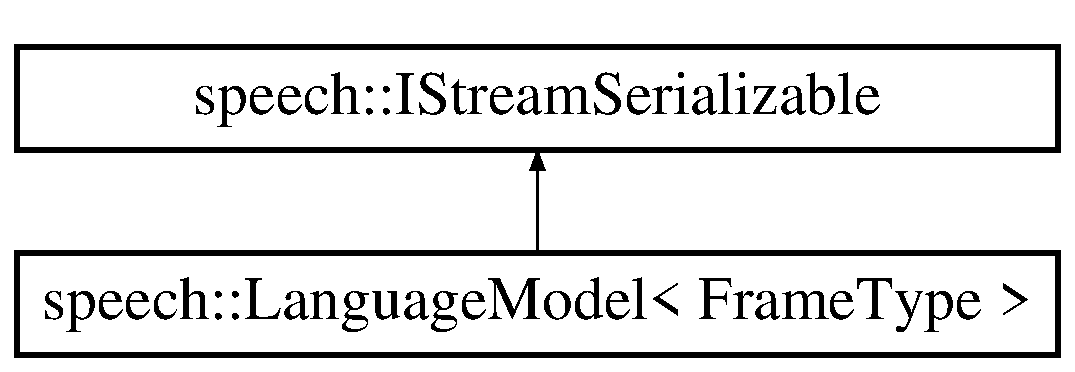
\includegraphics[height=2.000000cm]{classspeech_1_1LanguageModel}
\end{center}
\end{figure}
\subsection*{Public Member Functions}
\begin{DoxyCompactItemize}
\item 
\hypertarget{classspeech_1_1LanguageModel_a653f37a791e75e9ea968d58b6ee7d2fa}{{\bfseries Language\+Model} (std\+::istream \&in)}\label{classspeech_1_1LanguageModel_a653f37a791e75e9ea968d58b6ee7d2fa}

\item 
\hypertarget{classspeech_1_1LanguageModel_a810070486190924d9f9ba1afb3fe61c2}{{\bfseries Language\+Model} (shared\+\_\+ptr$<$ \hyperlink{classspeech_1_1vectorizer_1_1IVectorizer}{I\+Vectorizer}$<$ Frame\+Type $>$$>$ vectorizer, shared\+\_\+ptr$<$ \hyperlink{classspeech_1_1clustering_1_1IClusteringMethod}{clustering\+::\+I\+Clustering\+Method} $>$ clustering\+Method, shared\+\_\+ptr$<$ \hyperlink{classspeech_1_1spelling_1_1ISpellingTranscription}{spelling\+::\+I\+Spelling\+Transcription} $>$ spelling\+Transcription)}\label{classspeech_1_1LanguageModel_a810070486190924d9f9ba1afb3fe61c2}

\item 
void \hyperlink{classspeech_1_1LanguageModel_a07bc11f505b763e363748e7e1533615c}{fit} (vector$<$ \hyperlink{classspeech_1_1raw__data_1_1DataSource}{Data\+Source}$<$ Frame\+Type $>$$>$ \&data\+Sources, vector$<$ std\+::string $>$ \&transcriptions)
\item 
std\+::string \hyperlink{classspeech_1_1LanguageModel_ada9a59cc5f394d8ddecb650c0f334d87}{predict} (\hyperlink{classspeech_1_1raw__data_1_1DataSource}{Data\+Source}$<$ Frame\+Type $>$ \&data\+Source)
\item 
shared\+\_\+ptr$<$ \hyperlink{classspeech_1_1vectorizer_1_1IVectorizer}{I\+Vectorizer}\\*
$<$ Frame\+Type $>$ $>$ \hyperlink{classspeech_1_1LanguageModel_adbcee84dfcd012a9c9a12fc5dde7f3f6}{get\+Vectorizer} ()
\item 
shared\+\_\+ptr\\*
$<$ \hyperlink{classspeech_1_1clustering_1_1IClusteringMethod}{clustering\+::\+I\+Clustering\+Method} $>$ \hyperlink{classspeech_1_1LanguageModel_afb61fb7cf00950c3c85ed2860c17d83c}{get\+Clustering\+Method} ()
\item 
shared\+\_\+ptr\\*
$<$ \hyperlink{classspeech_1_1spelling_1_1ISpellingTranscription}{spelling\+::\+I\+Spelling\+Transcription} $>$ \hyperlink{classspeech_1_1LanguageModel_a0c5dab5aad9bb4dabc92bedbce99cfb6}{get\+Spelling\+Transcription} ()
\item 
virtual void \hyperlink{classspeech_1_1LanguageModel_ae3c30d0a1a1a5e60fd69954b432766fa}{serialize} (std\+::ostream \&out) const 
\end{DoxyCompactItemize}
\subsection*{Protected Attributes}
\begin{DoxyCompactItemize}
\item 
\hypertarget{classspeech_1_1LanguageModel_a5929f6de00b952d3094c8dd7bb240d05}{shared\+\_\+ptr$<$ \hyperlink{classspeech_1_1vectorizer_1_1IVectorizer}{I\+Vectorizer}\\*
$<$ Frame\+Type $>$ $>$ {\bfseries vectorizer} = nullptr}\label{classspeech_1_1LanguageModel_a5929f6de00b952d3094c8dd7bb240d05}

\item 
\hypertarget{classspeech_1_1LanguageModel_ac846feac8765604343d901e35de07c2a}{shared\+\_\+ptr\\*
$<$ \hyperlink{classspeech_1_1clustering_1_1IClusteringMethod}{clustering\+::\+I\+Clustering\+Method} $>$ {\bfseries clustering\+Method} = nullptr}\label{classspeech_1_1LanguageModel_ac846feac8765604343d901e35de07c2a}

\item 
\hypertarget{classspeech_1_1LanguageModel_a20b08c539071cd3dcbd49e59c3bc08f2}{shared\+\_\+ptr\\*
$<$ \hyperlink{classspeech_1_1spelling_1_1ISpellingTranscription}{spelling\+::\+I\+Spelling\+Transcription} $>$ {\bfseries spelling\+Transcription} = nullptr}\label{classspeech_1_1LanguageModel_a20b08c539071cd3dcbd49e59c3bc08f2}

\end{DoxyCompactItemize}


\subsection{Detailed Description}
\subsubsection*{template$<$typename Frame\+Type$>$class speech\+::\+Language\+Model$<$ Frame\+Type $>$}

It is a representation of the language model which is built from the clustering method and a method which converts labeled signals into textual representation (we call it spelling transcription) 

\subsection{Member Function Documentation}
\hypertarget{classspeech_1_1LanguageModel_a07bc11f505b763e363748e7e1533615c}{\index{speech\+::\+Language\+Model@{speech\+::\+Language\+Model}!fit@{fit}}
\index{fit@{fit}!speech\+::\+Language\+Model@{speech\+::\+Language\+Model}}
\subsubsection[{fit}]{\setlength{\rightskip}{0pt plus 5cm}template$<$typename Frame\+Type $>$ void {\bf speech\+::\+Language\+Model}$<$ Frame\+Type $>$\+::fit (
\begin{DoxyParamCaption}
\item[{vector$<$ {\bf Data\+Source}$<$ Frame\+Type $>$$>$ \&}]{data\+Sources, }
\item[{vector$<$ std\+::string $>$ \&}]{transcriptions}
\end{DoxyParamCaption}
)}}\label{classspeech_1_1LanguageModel_a07bc11f505b763e363748e7e1533615c}
Fits all model components 
\begin{DoxyParams}{Parameters}
{\em data\+Sources} & collection of data sources \\
\hline
{\em transcriptions} & collection of transcriptions for each provided data source \\
\hline
\end{DoxyParams}
\hypertarget{classspeech_1_1LanguageModel_afb61fb7cf00950c3c85ed2860c17d83c}{\index{speech\+::\+Language\+Model@{speech\+::\+Language\+Model}!get\+Clustering\+Method@{get\+Clustering\+Method}}
\index{get\+Clustering\+Method@{get\+Clustering\+Method}!speech\+::\+Language\+Model@{speech\+::\+Language\+Model}}
\subsubsection[{get\+Clustering\+Method}]{\setlength{\rightskip}{0pt plus 5cm}template$<$typename Frame\+Type $>$ shared\+\_\+ptr$<${\bf clustering\+::\+I\+Clustering\+Method}$>$ {\bf speech\+::\+Language\+Model}$<$ Frame\+Type $>$\+::get\+Clustering\+Method (
\begin{DoxyParamCaption}
{}
\end{DoxyParamCaption}
)\hspace{0.3cm}{\ttfamily [inline]}}}\label{classspeech_1_1LanguageModel_afb61fb7cf00950c3c85ed2860c17d83c}
Gets shared pointer to the clustering method used by the model

\begin{DoxyReturn}{Returns}
instance of the clustering method 
\end{DoxyReturn}
\hypertarget{classspeech_1_1LanguageModel_a0c5dab5aad9bb4dabc92bedbce99cfb6}{\index{speech\+::\+Language\+Model@{speech\+::\+Language\+Model}!get\+Spelling\+Transcription@{get\+Spelling\+Transcription}}
\index{get\+Spelling\+Transcription@{get\+Spelling\+Transcription}!speech\+::\+Language\+Model@{speech\+::\+Language\+Model}}
\subsubsection[{get\+Spelling\+Transcription}]{\setlength{\rightskip}{0pt plus 5cm}template$<$typename Frame\+Type $>$ shared\+\_\+ptr$<${\bf spelling\+::\+I\+Spelling\+Transcription}$>$ {\bf speech\+::\+Language\+Model}$<$ Frame\+Type $>$\+::get\+Spelling\+Transcription (
\begin{DoxyParamCaption}
{}
\end{DoxyParamCaption}
)\hspace{0.3cm}{\ttfamily [inline]}}}\label{classspeech_1_1LanguageModel_a0c5dab5aad9bb4dabc92bedbce99cfb6}
Gets shared pointer to the spelling transcription used by the model

\begin{DoxyReturn}{Returns}
instance of the spelling transcription 
\end{DoxyReturn}
\hypertarget{classspeech_1_1LanguageModel_adbcee84dfcd012a9c9a12fc5dde7f3f6}{\index{speech\+::\+Language\+Model@{speech\+::\+Language\+Model}!get\+Vectorizer@{get\+Vectorizer}}
\index{get\+Vectorizer@{get\+Vectorizer}!speech\+::\+Language\+Model@{speech\+::\+Language\+Model}}
\subsubsection[{get\+Vectorizer}]{\setlength{\rightskip}{0pt plus 5cm}template$<$typename Frame\+Type $>$ shared\+\_\+ptr$<${\bf I\+Vectorizer}$<$Frame\+Type$>$ $>$ {\bf speech\+::\+Language\+Model}$<$ Frame\+Type $>$\+::get\+Vectorizer (
\begin{DoxyParamCaption}
{}
\end{DoxyParamCaption}
)\hspace{0.3cm}{\ttfamily [inline]}}}\label{classspeech_1_1LanguageModel_adbcee84dfcd012a9c9a12fc5dde7f3f6}
Gets shared pointer to the vectorizer instance used by the model

\begin{DoxyReturn}{Returns}
instance of the vectorizer 
\end{DoxyReturn}
\hypertarget{classspeech_1_1LanguageModel_ada9a59cc5f394d8ddecb650c0f334d87}{\index{speech\+::\+Language\+Model@{speech\+::\+Language\+Model}!predict@{predict}}
\index{predict@{predict}!speech\+::\+Language\+Model@{speech\+::\+Language\+Model}}
\subsubsection[{predict}]{\setlength{\rightskip}{0pt plus 5cm}template$<$typename Frame\+Type $>$ std\+::string {\bf speech\+::\+Language\+Model}$<$ Frame\+Type $>$\+::predict (
\begin{DoxyParamCaption}
\item[{{\bf Data\+Source}$<$ Frame\+Type $>$ \&}]{data\+Source}
\end{DoxyParamCaption}
)}}\label{classspeech_1_1LanguageModel_ada9a59cc5f394d8ddecb650c0f334d87}
Predicts the sentence from given data source samples 
\begin{DoxyParams}{Parameters}
{\em data\+Source} & referene to the data source\\
\hline
\end{DoxyParams}
\begin{DoxyReturn}{Returns}
predicted sentence 
\end{DoxyReturn}
\hypertarget{classspeech_1_1LanguageModel_ae3c30d0a1a1a5e60fd69954b432766fa}{\index{speech\+::\+Language\+Model@{speech\+::\+Language\+Model}!serialize@{serialize}}
\index{serialize@{serialize}!speech\+::\+Language\+Model@{speech\+::\+Language\+Model}}
\subsubsection[{serialize}]{\setlength{\rightskip}{0pt plus 5cm}template$<$typename Frame\+Type $>$ void {\bf speech\+::\+Language\+Model}$<$ Frame\+Type $>$\+::serialize (
\begin{DoxyParamCaption}
\item[{std\+::ostream \&}]{out}
\end{DoxyParamCaption}
) const\hspace{0.3cm}{\ttfamily [virtual]}}}\label{classspeech_1_1LanguageModel_ae3c30d0a1a1a5e60fd69954b432766fa}
Writes an object to given stream 
\begin{DoxyParams}{Parameters}
{\em out} & output stream \\
\hline
\end{DoxyParams}


Implements \hyperlink{classspeech_1_1IStreamSerializable_a891561ebe3e4eb5411e613b28bc2c982}{speech\+::\+I\+Stream\+Serializable}.



The documentation for this class was generated from the following files\+:\begin{DoxyCompactItemize}
\item 
/home/kacper/\+Projects/speech-\/recognition/src/speech/Language\+Model.\+h\item 
/home/kacper/\+Projects/speech-\/recognition/src/speech/Language\+Model.\+cpp\end{DoxyCompactItemize}

\hypertarget{classspeech_1_1raw__data_1_1filtering_1_1MaxFrequenciesFilter}{\section{speech\+:\+:raw\+\_\+data\+:\+:filtering\+:\+:Max\+Frequencies\+Filter$<$ Frame\+Type $>$ Class Template Reference}
\label{classspeech_1_1raw__data_1_1filtering_1_1MaxFrequenciesFilter}\index{speech\+::raw\+\_\+data\+::filtering\+::\+Max\+Frequencies\+Filter$<$ Frame\+Type $>$@{speech\+::raw\+\_\+data\+::filtering\+::\+Max\+Frequencies\+Filter$<$ Frame\+Type $>$}}
}
Inheritance diagram for speech\+:\+:raw\+\_\+data\+:\+:filtering\+:\+:Max\+Frequencies\+Filter$<$ Frame\+Type $>$\+:\begin{figure}[H]
\begin{center}
\leavevmode
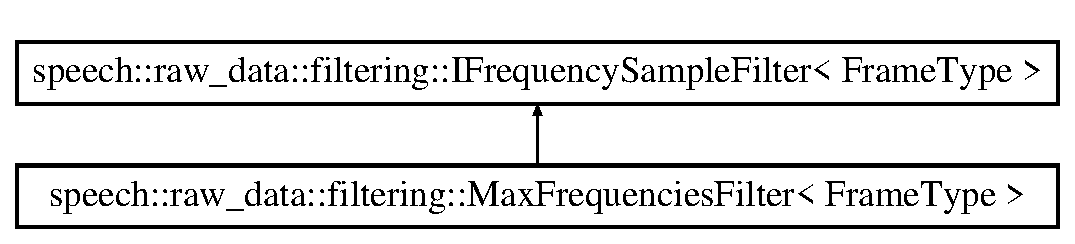
\includegraphics[height=2.000000cm]{classspeech_1_1raw__data_1_1filtering_1_1MaxFrequenciesFilter}
\end{center}
\end{figure}
\subsection*{Public Member Functions}
\begin{DoxyCompactItemize}
\item 
\hypertarget{classspeech_1_1raw__data_1_1filtering_1_1MaxFrequenciesFilter_a8f829010be02bb04a13ebdd99051887b}{{\bfseries Max\+Frequencies\+Filter} (int n)}\label{classspeech_1_1raw__data_1_1filtering_1_1MaxFrequenciesFilter_a8f829010be02bb04a13ebdd99051887b}

\item 
\hypertarget{classspeech_1_1raw__data_1_1filtering_1_1MaxFrequenciesFilter_a788c9b1a1476fd2b612b83cda4a09ff4}{virtual \hyperlink{classspeech_1_1raw__data_1_1FrequencySample}{Frequency\+Sample}\\*
$<$ Frame\+Type $>$ {\bfseries filter} (const \hyperlink{classspeech_1_1raw__data_1_1FrequencySample}{Frequency\+Sample}$<$ Frame\+Type $>$ \&sample)}\label{classspeech_1_1raw__data_1_1filtering_1_1MaxFrequenciesFilter_a788c9b1a1476fd2b612b83cda4a09ff4}

\end{DoxyCompactItemize}
\subsection*{Protected Attributes}
\begin{DoxyCompactItemize}
\item 
\hypertarget{classspeech_1_1raw__data_1_1filtering_1_1MaxFrequenciesFilter_a053feca5518f5e2c8f394f27c75e5163}{int {\bfseries n}}\label{classspeech_1_1raw__data_1_1filtering_1_1MaxFrequenciesFilter_a053feca5518f5e2c8f394f27c75e5163}

\end{DoxyCompactItemize}
\subsection*{Static Protected Attributes}
\begin{DoxyCompactItemize}
\item 
\hypertarget{classspeech_1_1raw__data_1_1filtering_1_1MaxFrequenciesFilter_ae05c85e27458890c3a53f26e0ea442bc}{static double constexpr {\bfseries E\+P\+S} = 1e-\/2}\label{classspeech_1_1raw__data_1_1filtering_1_1MaxFrequenciesFilter_ae05c85e27458890c3a53f26e0ea442bc}

\end{DoxyCompactItemize}


The documentation for this class was generated from the following files\+:\begin{DoxyCompactItemize}
\item 
/home/kacper/\+Projects/speech-\/recognition/src/speech/raw\+\_\+data/filtering/Max\+Frequencies\+Filter.\+h\item 
/home/kacper/\+Projects/speech-\/recognition/src/speech/raw\+\_\+data/filtering/Max\+Frequencies\+Filter.\+cpp\end{DoxyCompactItemize}

\hypertarget{classspeech_1_1vectorizer_1_1MaxFrequencyVectorizer}{\section{speech\+:\+:vectorizer\+:\+:Max\+Frequency\+Vectorizer$<$ Frame\+Type $>$ Class Template Reference}
\label{classspeech_1_1vectorizer_1_1MaxFrequencyVectorizer}\index{speech\+::vectorizer\+::\+Max\+Frequency\+Vectorizer$<$ Frame\+Type $>$@{speech\+::vectorizer\+::\+Max\+Frequency\+Vectorizer$<$ Frame\+Type $>$}}
}


{\ttfamily \#include $<$Max\+Frequency\+Vectorizer.\+h$>$}

Inheritance diagram for speech\+:\+:vectorizer\+:\+:Max\+Frequency\+Vectorizer$<$ Frame\+Type $>$\+:\begin{figure}[H]
\begin{center}
\leavevmode
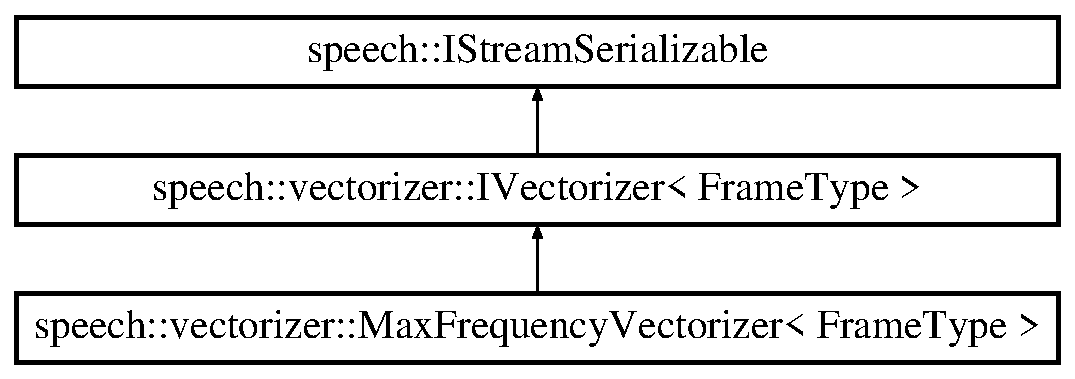
\includegraphics[height=3.000000cm]{classspeech_1_1vectorizer_1_1MaxFrequencyVectorizer}
\end{center}
\end{figure}
\subsection*{Public Member Functions}
\begin{DoxyCompactItemize}
\item 
\hypertarget{classspeech_1_1vectorizer_1_1MaxFrequencyVectorizer_a5f2209fb1be3ddfa5786678154156b83}{{\bfseries Max\+Frequency\+Vectorizer} (int n)}\label{classspeech_1_1vectorizer_1_1MaxFrequencyVectorizer_a5f2209fb1be3ddfa5786678154156b83}

\item 
\hypertarget{classspeech_1_1vectorizer_1_1MaxFrequencyVectorizer_a516e583601993b370f6a65b0adc4603f}{{\bfseries Max\+Frequency\+Vectorizer} (std\+::istream \&in)}\label{classspeech_1_1vectorizer_1_1MaxFrequencyVectorizer_a516e583601993b370f6a65b0adc4603f}

\item 
virtual std\+::valarray$<$ double $>$ \hyperlink{classspeech_1_1vectorizer_1_1MaxFrequencyVectorizer_a9463cc7d335fdc5d181d2dffbd488a12}{vectorize} (\hyperlink{classspeech_1_1raw__data_1_1FrequencySample}{Frequency\+Sample}$<$ Frame\+Type $>$ \&sample) override
\item 
virtual void \hyperlink{classspeech_1_1vectorizer_1_1MaxFrequencyVectorizer_a1fdb7b7544a6386e64e8df49b644a13c}{serialize} (std\+::ostream \&out) const override
\item 
virtual int \hyperlink{classspeech_1_1vectorizer_1_1MaxFrequencyVectorizer_af92f2750d71a14cbc74d8508f8dbb354}{get\+Vector\+Size} () const 
\end{DoxyCompactItemize}
\subsection*{Static Public Attributes}
\begin{DoxyCompactItemize}
\item 
\hypertarget{classspeech_1_1vectorizer_1_1MaxFrequencyVectorizer_aac82e0f57f615cafb37845b5a023f699}{static const uint32\+\_\+t {\bfseries T\+Y\+P\+E\+\_\+\+I\+D\+E\+N\+T\+I\+F\+I\+E\+R} = 0x00100001}\label{classspeech_1_1vectorizer_1_1MaxFrequencyVectorizer_aac82e0f57f615cafb37845b5a023f699}

\end{DoxyCompactItemize}
\subsection*{Additional Inherited Members}


\subsection{Detailed Description}
\subsubsection*{template$<$typename Frame\+Type$>$class speech\+::vectorizer\+::\+Max\+Frequency\+Vectorizer$<$ Frame\+Type $>$}

Vectorizer converting raw signal into vectors of fixed size containing frequencies with maximal amplitude. \begin{DoxyRefDesc}{Deprecated}
\item[\hyperlink{deprecated__deprecated000002}{Deprecated}]\end{DoxyRefDesc}


\subsection{Member Function Documentation}
\hypertarget{classspeech_1_1vectorizer_1_1MaxFrequencyVectorizer_af92f2750d71a14cbc74d8508f8dbb354}{\index{speech\+::vectorizer\+::\+Max\+Frequency\+Vectorizer@{speech\+::vectorizer\+::\+Max\+Frequency\+Vectorizer}!get\+Vector\+Size@{get\+Vector\+Size}}
\index{get\+Vector\+Size@{get\+Vector\+Size}!speech\+::vectorizer\+::\+Max\+Frequency\+Vectorizer@{speech\+::vectorizer\+::\+Max\+Frequency\+Vectorizer}}
\subsubsection[{get\+Vector\+Size}]{\setlength{\rightskip}{0pt plus 5cm}template$<$typename Frame\+Type $>$ int {\bf speech\+::vectorizer\+::\+Max\+Frequency\+Vectorizer}$<$ Frame\+Type $>$\+::get\+Vector\+Size (
\begin{DoxyParamCaption}
{}
\end{DoxyParamCaption}
) const\hspace{0.3cm}{\ttfamily [virtual]}}}\label{classspeech_1_1vectorizer_1_1MaxFrequencyVectorizer_af92f2750d71a14cbc74d8508f8dbb354}
Gets the size of the output vector produced by the vectorizer.

\begin{DoxyReturn}{Returns}
size of the produced vector 
\end{DoxyReturn}


Implements \hyperlink{classspeech_1_1vectorizer_1_1IVectorizer_abe20529a1586c072783f42476ad7ab69}{speech\+::vectorizer\+::\+I\+Vectorizer$<$ Frame\+Type $>$}.

\hypertarget{classspeech_1_1vectorizer_1_1MaxFrequencyVectorizer_a1fdb7b7544a6386e64e8df49b644a13c}{\index{speech\+::vectorizer\+::\+Max\+Frequency\+Vectorizer@{speech\+::vectorizer\+::\+Max\+Frequency\+Vectorizer}!serialize@{serialize}}
\index{serialize@{serialize}!speech\+::vectorizer\+::\+Max\+Frequency\+Vectorizer@{speech\+::vectorizer\+::\+Max\+Frequency\+Vectorizer}}
\subsubsection[{serialize}]{\setlength{\rightskip}{0pt plus 5cm}template$<$typename Frame\+Type $>$ void {\bf speech\+::vectorizer\+::\+Max\+Frequency\+Vectorizer}$<$ Frame\+Type $>$\+::serialize (
\begin{DoxyParamCaption}
\item[{std\+::ostream \&}]{out}
\end{DoxyParamCaption}
) const\hspace{0.3cm}{\ttfamily [override]}, {\ttfamily [virtual]}}}\label{classspeech_1_1vectorizer_1_1MaxFrequencyVectorizer_a1fdb7b7544a6386e64e8df49b644a13c}
Serializes the vectorizer into given stream. 
\begin{DoxyParams}{Parameters}
{\em out} & output stream \\
\hline
\end{DoxyParams}


Implements \hyperlink{classspeech_1_1vectorizer_1_1IVectorizer_aa8285bbd275c31ae1ce48d294400dea9}{speech\+::vectorizer\+::\+I\+Vectorizer$<$ Frame\+Type $>$}.

\hypertarget{classspeech_1_1vectorizer_1_1MaxFrequencyVectorizer_a9463cc7d335fdc5d181d2dffbd488a12}{\index{speech\+::vectorizer\+::\+Max\+Frequency\+Vectorizer@{speech\+::vectorizer\+::\+Max\+Frequency\+Vectorizer}!vectorize@{vectorize}}
\index{vectorize@{vectorize}!speech\+::vectorizer\+::\+Max\+Frequency\+Vectorizer@{speech\+::vectorizer\+::\+Max\+Frequency\+Vectorizer}}
\subsubsection[{vectorize}]{\setlength{\rightskip}{0pt plus 5cm}template$<$typename Frame\+Type $>$ std\+::valarray$<$ double $>$ {\bf speech\+::vectorizer\+::\+Max\+Frequency\+Vectorizer}$<$ Frame\+Type $>$\+::vectorize (
\begin{DoxyParamCaption}
\item[{{\bf Frequency\+Sample}$<$ Frame\+Type $>$ \&}]{sample}
\end{DoxyParamCaption}
)\hspace{0.3cm}{\ttfamily [override]}, {\ttfamily [virtual]}}}\label{classspeech_1_1vectorizer_1_1MaxFrequencyVectorizer_a9463cc7d335fdc5d181d2dffbd488a12}
Projects given sample into feature space. Each vector needs to have exactly same size. 
\begin{DoxyParams}{Parameters}
{\em sample} & single sample to be vectorized\\
\hline
\end{DoxyParams}
\begin{DoxyReturn}{Returns}
the projection of vector in a feature space 
\end{DoxyReturn}


Implements \hyperlink{classspeech_1_1vectorizer_1_1IVectorizer_a00d2ba71ec5c447780ffb0a29bfc9085}{speech\+::vectorizer\+::\+I\+Vectorizer$<$ Frame\+Type $>$}.



The documentation for this class was generated from the following files\+:\begin{DoxyCompactItemize}
\item 
/home/kacper/\+Projects/speech-\/recognition/src/speech/vectorizer/Max\+Frequency\+Vectorizer.\+h\item 
/home/kacper/\+Projects/speech-\/recognition/src/speech/vectorizer/Max\+Frequency\+Vectorizer.\+cpp\end{DoxyCompactItemize}

\hypertarget{classspeech_1_1metric_1_1MaximumDistance}{\section{speech\+:\+:metric\+:\+:Maximum\+Distance Class Reference}
\label{classspeech_1_1metric_1_1MaximumDistance}\index{speech\+::metric\+::\+Maximum\+Distance@{speech\+::metric\+::\+Maximum\+Distance}}
}


{\ttfamily \#include $<$Maximum\+Distance.\+h$>$}

Inheritance diagram for speech\+:\+:metric\+:\+:Maximum\+Distance\+:\begin{figure}[H]
\begin{center}
\leavevmode
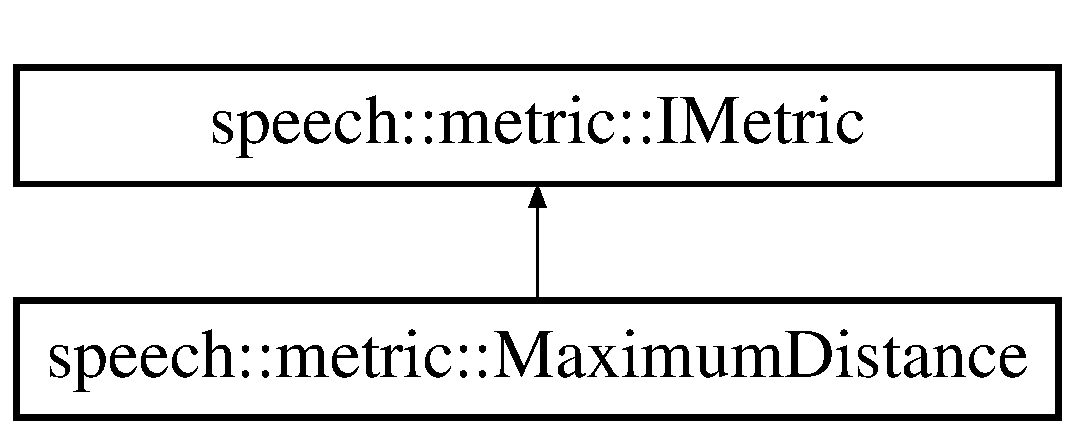
\includegraphics[height=2.000000cm]{classspeech_1_1metric_1_1MaximumDistance}
\end{center}
\end{figure}
\subsection*{Public Member Functions}
\begin{DoxyCompactItemize}
\item 
virtual double \hyperlink{classspeech_1_1metric_1_1MaximumDistance_aa2c39fc82d79a701aecb8982ac0f2eaf}{operator()} (const std\+::valarray$<$ double $>$ \&v1, const std\+::valarray$<$ double $>$ \&v2)
\end{DoxyCompactItemize}


\subsection{Detailed Description}
A metric calculating maximum distance between two given vectors\+: d(x, y) = max\+\_\+i($\vert$x\+\_\+i -\/ y\+\_\+i$\vert$) 

\subsection{Member Function Documentation}
\hypertarget{classspeech_1_1metric_1_1MaximumDistance_aa2c39fc82d79a701aecb8982ac0f2eaf}{\index{speech\+::metric\+::\+Maximum\+Distance@{speech\+::metric\+::\+Maximum\+Distance}!operator()@{operator()}}
\index{operator()@{operator()}!speech\+::metric\+::\+Maximum\+Distance@{speech\+::metric\+::\+Maximum\+Distance}}
\subsubsection[{operator()}]{\setlength{\rightskip}{0pt plus 5cm}double speech\+::metric\+::\+Maximum\+Distance\+::operator() (
\begin{DoxyParamCaption}
\item[{const std\+::valarray$<$ double $>$ \&}]{v1, }
\item[{const std\+::valarray$<$ double $>$ \&}]{v2}
\end{DoxyParamCaption}
)\hspace{0.3cm}{\ttfamily [virtual]}}}\label{classspeech_1_1metric_1_1MaximumDistance_aa2c39fc82d79a701aecb8982ac0f2eaf}
Calculates a distance between two vectors. \begin{DoxyReturn}{Returns}
a distance 
\end{DoxyReturn}


Implements \hyperlink{classspeech_1_1metric_1_1IMetric_af15c579c0870b67e862945b6918bc14e}{speech\+::metric\+::\+I\+Metric}.



The documentation for this class was generated from the following files\+:\begin{DoxyCompactItemize}
\item 
/home/kacper/\+Projects/speech-\/recognition/src/speech/metric/Maximum\+Distance.\+h\item 
/home/kacper/\+Projects/speech-\/recognition/src/speech/metric/Maximum\+Distance.\+cpp\end{DoxyCompactItemize}

\hypertarget{classspeech_1_1vectorizer_1_1MFCCVectorizer_1_1MelFilter}{\section{speech\+:\+:vectorizer\+:\+:M\+F\+C\+C\+Vectorizer$<$ Frame\+Type $>$\+:\+:Mel\+Filter Class Reference}
\label{classspeech_1_1vectorizer_1_1MFCCVectorizer_1_1MelFilter}\index{speech\+::vectorizer\+::\+M\+F\+C\+C\+Vectorizer$<$ Frame\+Type $>$\+::\+Mel\+Filter@{speech\+::vectorizer\+::\+M\+F\+C\+C\+Vectorizer$<$ Frame\+Type $>$\+::\+Mel\+Filter}}
}


{\ttfamily \#include $<$M\+F\+C\+C\+Vectorizer.\+h$>$}

\subsection*{Public Member Functions}
\begin{DoxyCompactItemize}
\item 
\hyperlink{classspeech_1_1vectorizer_1_1MFCCVectorizer_1_1MelFilter_a406c5493a1eaeea4586c372ddb0dbd5c}{Mel\+Filter} (double start\+Frequency, double end\+Frequency)
\item 
double \hyperlink{classspeech_1_1vectorizer_1_1MFCCVectorizer_1_1MelFilter_a332be225c09e3c12e2a05f9a61401e96}{operator()} (\hyperlink{classspeech_1_1raw__data_1_1Spectrum}{Spectrum} \&spectrum)
\item 
double \hyperlink{classspeech_1_1vectorizer_1_1MFCCVectorizer_1_1MelFilter_a024b85d403d333f6f7649e11de0bf257}{get\+Index\+Coeff} (int index, int start\+Index, int center\+Index, int end\+Index)
\item 
\hypertarget{classspeech_1_1vectorizer_1_1MFCCVectorizer_1_1MelFilter_af41ba8e8dc53e80cbaf45509874e7655}{double {\bfseries get\+Frequency\+Coeff} (double frequency, double start\+Frequency, double center\+Frequency, double end\+Frequency)}\label{classspeech_1_1vectorizer_1_1MFCCVectorizer_1_1MelFilter_af41ba8e8dc53e80cbaf45509874e7655}

\end{DoxyCompactItemize}


\subsection{Detailed Description}
\subsubsection*{template$<$typename Frame\+Type$>$class speech\+::vectorizer\+::\+M\+F\+C\+C\+Vectorizer$<$ Frame\+Type $>$\+::\+Mel\+Filter}

A triangular filter used in M\+F\+C\+C calculating 

\subsection{Constructor \& Destructor Documentation}
\hypertarget{classspeech_1_1vectorizer_1_1MFCCVectorizer_1_1MelFilter_a406c5493a1eaeea4586c372ddb0dbd5c}{\index{speech\+::vectorizer\+::\+M\+F\+C\+C\+Vectorizer\+::\+Mel\+Filter@{speech\+::vectorizer\+::\+M\+F\+C\+C\+Vectorizer\+::\+Mel\+Filter}!Mel\+Filter@{Mel\+Filter}}
\index{Mel\+Filter@{Mel\+Filter}!speech\+::vectorizer\+::\+M\+F\+C\+C\+Vectorizer\+::\+Mel\+Filter@{speech\+::vectorizer\+::\+M\+F\+C\+C\+Vectorizer\+::\+Mel\+Filter}}
\subsubsection[{Mel\+Filter}]{\setlength{\rightskip}{0pt plus 5cm}template$<$typename Frame\+Type $>$ {\bf speech\+::vectorizer\+::\+M\+F\+C\+C\+Vectorizer}$<$ Frame\+Type $>$\+::Mel\+Filter\+::\+Mel\+Filter (
\begin{DoxyParamCaption}
\item[{double}]{start\+Frequency, }
\item[{double}]{end\+Frequency}
\end{DoxyParamCaption}
)\hspace{0.3cm}{\ttfamily [inline]}}}\label{classspeech_1_1vectorizer_1_1MFCCVectorizer_1_1MelFilter_a406c5493a1eaeea4586c372ddb0dbd5c}
Constructs a filter non-\/zero in given boundaries 
\begin{DoxyParams}{Parameters}
{\em start\+Frequenfcy} & begin frequency in herzs \\
\hline
{\em end\+Frequency} & end frequency in herzs \\
\hline
\end{DoxyParams}


\subsection{Member Function Documentation}
\hypertarget{classspeech_1_1vectorizer_1_1MFCCVectorizer_1_1MelFilter_a024b85d403d333f6f7649e11de0bf257}{\index{speech\+::vectorizer\+::\+M\+F\+C\+C\+Vectorizer\+::\+Mel\+Filter@{speech\+::vectorizer\+::\+M\+F\+C\+C\+Vectorizer\+::\+Mel\+Filter}!get\+Index\+Coeff@{get\+Index\+Coeff}}
\index{get\+Index\+Coeff@{get\+Index\+Coeff}!speech\+::vectorizer\+::\+M\+F\+C\+C\+Vectorizer\+::\+Mel\+Filter@{speech\+::vectorizer\+::\+M\+F\+C\+C\+Vectorizer\+::\+Mel\+Filter}}
\subsubsection[{get\+Index\+Coeff}]{\setlength{\rightskip}{0pt plus 5cm}template$<$typename Frame\+Type $>$ double {\bf speech\+::vectorizer\+::\+M\+F\+C\+C\+Vectorizer}$<$ Frame\+Type $>$\+::Mel\+Filter\+::get\+Index\+Coeff (
\begin{DoxyParamCaption}
\item[{int}]{index, }
\item[{int}]{start\+Index, }
\item[{int}]{center\+Index, }
\item[{int}]{end\+Index}
\end{DoxyParamCaption}
)\hspace{0.3cm}{\ttfamily [inline]}}}\label{classspeech_1_1vectorizer_1_1MFCCVectorizer_1_1MelFilter_a024b85d403d333f6f7649e11de0bf257}
Calculates the weight of the given index 
\begin{DoxyParams}{Parameters}
{\em index} & current index \\
\hline
{\em start\+Index} & the beginning of this particular filter \\
\hline
{\em center\+Index} & the middle of this particular filter \\
\hline
{\em end\+Index} & the end of this particular filter \\
\hline
\end{DoxyParams}
\hypertarget{classspeech_1_1vectorizer_1_1MFCCVectorizer_1_1MelFilter_a332be225c09e3c12e2a05f9a61401e96}{\index{speech\+::vectorizer\+::\+M\+F\+C\+C\+Vectorizer\+::\+Mel\+Filter@{speech\+::vectorizer\+::\+M\+F\+C\+C\+Vectorizer\+::\+Mel\+Filter}!operator()@{operator()}}
\index{operator()@{operator()}!speech\+::vectorizer\+::\+M\+F\+C\+C\+Vectorizer\+::\+Mel\+Filter@{speech\+::vectorizer\+::\+M\+F\+C\+C\+Vectorizer\+::\+Mel\+Filter}}
\subsubsection[{operator()}]{\setlength{\rightskip}{0pt plus 5cm}template$<$typename Frame\+Type $>$ double {\bf speech\+::vectorizer\+::\+M\+F\+C\+C\+Vectorizer}$<$ Frame\+Type $>$\+::Mel\+Filter\+::operator() (
\begin{DoxyParamCaption}
\item[{{\bf Spectrum} \&}]{spectrum}
\end{DoxyParamCaption}
)\hspace{0.3cm}{\ttfamily [inline]}}}\label{classspeech_1_1vectorizer_1_1MFCCVectorizer_1_1MelFilter_a332be225c09e3c12e2a05f9a61401e96}
Calucates an energy in given spectrum 
\begin{DoxyParams}{Parameters}
{\em spectrum} & reference to Spectrum class object \\
\hline
\end{DoxyParams}
\begin{DoxyReturn}{Returns}
energy of this filter in given spectrum 
\end{DoxyReturn}


The documentation for this class was generated from the following file\+:\begin{DoxyCompactItemize}
\item 
/home/kacper/\+Projects/speech-\/recognition/src/speech/vectorizer/M\+F\+C\+C\+Vectorizer.\+h\end{DoxyCompactItemize}

\hypertarget{classspeech_1_1vectorizer_1_1MFCCVectorizer}{\section{speech\+:\+:vectorizer\+:\+:M\+F\+C\+C\+Vectorizer$<$ Frame\+Type $>$ Class Template Reference}
\label{classspeech_1_1vectorizer_1_1MFCCVectorizer}\index{speech\+::vectorizer\+::\+M\+F\+C\+C\+Vectorizer$<$ Frame\+Type $>$@{speech\+::vectorizer\+::\+M\+F\+C\+C\+Vectorizer$<$ Frame\+Type $>$}}
}


{\ttfamily \#include $<$M\+F\+C\+C\+Vectorizer.\+h$>$}

Inheritance diagram for speech\+:\+:vectorizer\+:\+:M\+F\+C\+C\+Vectorizer$<$ Frame\+Type $>$\+:\begin{figure}[H]
\begin{center}
\leavevmode
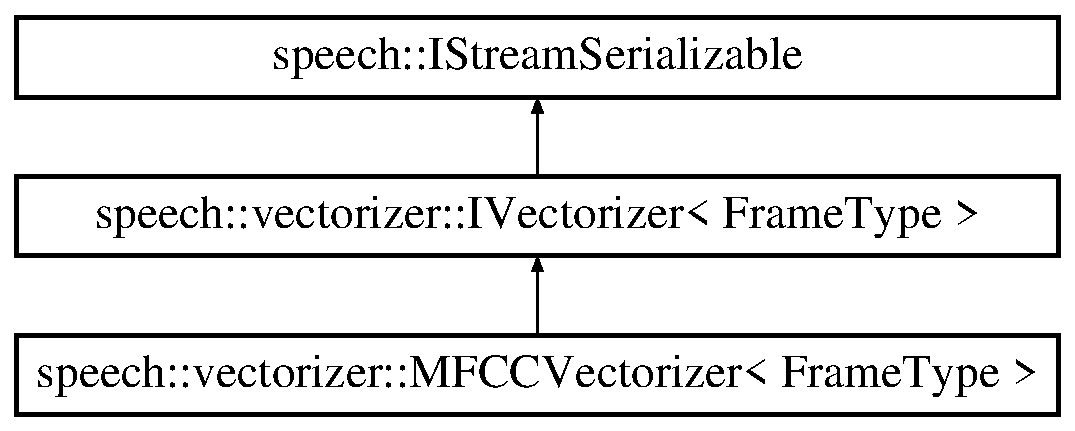
\includegraphics[height=3.000000cm]{classspeech_1_1vectorizer_1_1MFCCVectorizer}
\end{center}
\end{figure}
\subsection*{Classes}
\begin{DoxyCompactItemize}
\item 
class \hyperlink{classspeech_1_1vectorizer_1_1MFCCVectorizer_1_1MelFilter}{Mel\+Filter}
\end{DoxyCompactItemize}
\subsection*{Public Member Functions}
\begin{DoxyCompactItemize}
\item 
\hyperlink{classspeech_1_1vectorizer_1_1MFCCVectorizer_ababa626e7d260bdd7d3afb9694efe6a6}{M\+F\+C\+C\+Vectorizer} (std\+::istream \&in)
\item 
\hyperlink{classspeech_1_1vectorizer_1_1MFCCVectorizer_a84a36ac3b636e9f3460ba5bb0cb524e7}{M\+F\+C\+C\+Vectorizer} (int \hyperlink{classspeech_1_1vectorizer_1_1MFCCVectorizer_a179a54e359180354c417f980b222f1eb}{bins}, int \hyperlink{classspeech_1_1vectorizer_1_1MFCCVectorizer_a5f5083150768e6c9aad1777502e59a58}{cepstral\+Coefficients\+Number}, double min\+Frequency=64.\+0, double max\+Frequency=16000.\+0, int window\+Ms\+Size=20, int offset\+Ms\+Size=10, double emphasis\+Factor=0.\+97)
\item 
virtual std\+::valarray$<$ double $>$ \hyperlink{classspeech_1_1vectorizer_1_1MFCCVectorizer_ad494d113915e9a5d0bbecda045cf8799}{vectorize} (\hyperlink{classspeech_1_1raw__data_1_1FrequencySample}{Frequency\+Sample}$<$ Frame\+Type $>$ \&sample)
\item 
virtual std\+::vector\\*
$<$ std\+::valarray$<$ double $>$ $>$ \hyperlink{classspeech_1_1vectorizer_1_1MFCCVectorizer_a21a1862ff866a77c540943f48a6511d2}{vectorize} (std\+::vector$<$ \hyperlink{classspeech_1_1raw__data_1_1FrequencySample}{Frequency\+Sample}$<$ Frame\+Type $>$$>$ \&samples) override
\item 
virtual std\+::vector\\*
$<$ std\+::valarray$<$ double $>$ $>$ \hyperlink{classspeech_1_1vectorizer_1_1MFCCVectorizer_a7faab008b85e4fd817a04194b6470e88}{vectorize} (\hyperlink{classspeech_1_1raw__data_1_1DataSource}{Data\+Source}$<$ Frame\+Type $>$ \&data\+Source) override
\item 
virtual void \hyperlink{classspeech_1_1vectorizer_1_1MFCCVectorizer_a5f266d0fc3ab4dd89a1d701531818930}{serialize} (std\+::ostream \&out) const 
\item 
virtual int \hyperlink{classspeech_1_1vectorizer_1_1MFCCVectorizer_a47475baa543b7fe77f227d1e0288b99d}{get\+Vector\+Size} () const 
\end{DoxyCompactItemize}
\subsection*{Static Public Attributes}
\begin{DoxyCompactItemize}
\item 
static const uint32\+\_\+t \hyperlink{classspeech_1_1vectorizer_1_1MFCCVectorizer_a43112849b3a53dcdeec39a9721e11364}{T\+Y\+P\+E\+\_\+\+I\+D\+E\+N\+T\+I\+F\+I\+E\+R} = 0x00100004
\end{DoxyCompactItemize}
\subsection*{Protected Member Functions}
\begin{DoxyCompactItemize}
\item 
double \hyperlink{classspeech_1_1vectorizer_1_1MFCCVectorizer_ac519c16aa05a93d8c9cfbeec6d90f9d9}{herz\+To\+Mel} (double frequency)
\item 
double \hyperlink{classspeech_1_1vectorizer_1_1MFCCVectorizer_ab92ba6f1f5e52befdbb6ce5d6e37b870}{mel\+To\+Herz} (double mels)
\item 
std\+::valarray$<$ double $>$ \hyperlink{classspeech_1_1vectorizer_1_1MFCCVectorizer_a2ef3bd222534d0b5f9b79d146de969af}{calculate\+Cepstrum\+Coefficients} (const \hyperlink{classspeech_1_1raw__data_1_1FrequencySample}{Frequency\+Sample}$<$ Frame\+Type $>$ \&sample)
\end{DoxyCompactItemize}
\subsection*{Protected Attributes}
\begin{DoxyCompactItemize}
\item 
int \hyperlink{classspeech_1_1vectorizer_1_1MFCCVectorizer_a179a54e359180354c417f980b222f1eb}{bins}
\item 
int \hyperlink{classspeech_1_1vectorizer_1_1MFCCVectorizer_a5f5083150768e6c9aad1777502e59a58}{cepstral\+Coefficients\+Number}
\item 
double \hyperlink{classspeech_1_1vectorizer_1_1MFCCVectorizer_aa457579c8cac5d821a9cc6881d08124b}{min\+Cepstrum\+Frequency}
\item 
double \hyperlink{classspeech_1_1vectorizer_1_1MFCCVectorizer_a50431c541e9cba136395055ffd076c70}{max\+Cepstrum\+Frequency}
\item 
\hyperlink{classspeech_1_1transform_1_1IFrequencyTransform}{I\+Frequency\+Transform}$<$ Frame\+Type $>$ $\ast$ \hyperlink{classspeech_1_1vectorizer_1_1MFCCVectorizer_ac63aa92505370502b5e7c456bf8a8255}{frequency\+Transform} = new \hyperlink{classspeech_1_1transform_1_1FastFourierTransform}{Fast\+Fourier\+Transform}$<$Frame\+Type$>$()
\item 
std\+::vector$<$ \hyperlink{classspeech_1_1vectorizer_1_1MFCCVectorizer_1_1MelFilter}{Mel\+Filter} $>$ \hyperlink{classspeech_1_1vectorizer_1_1MFCCVectorizer_ab24511b7854870d534bdc408ddaf43bb}{filter\+Bank}
\item 
\hyperlink{classspeech_1_1raw__data_1_1filtering_1_1EmphasisFilter}{Emphasis\+Filter}$<$ Frame\+Type $>$ $\ast$ \hyperlink{classspeech_1_1vectorizer_1_1MFCCVectorizer_a36f6a48cc775f2b7d12f8fbfc103c448}{emphasis\+Filter}
\end{DoxyCompactItemize}


\subsection{Detailed Description}
\subsubsection*{template$<$typename Frame\+Type$>$class speech\+::vectorizer\+::\+M\+F\+C\+C\+Vectorizer$<$ Frame\+Type $>$}

Vectorizer using Mel Frequency Capstral Coefficients to describe a sound sample. \begin{DoxySeeAlso}{See also}
\href{http://webapp.etsi.org/workprogram/Report_WorkItem.asp?wki_id=18820}{\tt http\+://webapp.\+etsi.\+org/workprogram/\+Report\+\_\+\+Work\+Item.\+asp?wki\+\_\+id=18820} 
\end{DoxySeeAlso}


\subsection{Constructor \& Destructor Documentation}
\hypertarget{classspeech_1_1vectorizer_1_1MFCCVectorizer_ababa626e7d260bdd7d3afb9694efe6a6}{\index{speech\+::vectorizer\+::\+M\+F\+C\+C\+Vectorizer@{speech\+::vectorizer\+::\+M\+F\+C\+C\+Vectorizer}!M\+F\+C\+C\+Vectorizer@{M\+F\+C\+C\+Vectorizer}}
\index{M\+F\+C\+C\+Vectorizer@{M\+F\+C\+C\+Vectorizer}!speech\+::vectorizer\+::\+M\+F\+C\+C\+Vectorizer@{speech\+::vectorizer\+::\+M\+F\+C\+C\+Vectorizer}}
\subsubsection[{M\+F\+C\+C\+Vectorizer}]{\setlength{\rightskip}{0pt plus 5cm}template$<$typename Frame\+Type $>$ {\bf speech\+::vectorizer\+::\+M\+F\+C\+C\+Vectorizer}$<$ Frame\+Type $>$\+::{\bf M\+F\+C\+C\+Vectorizer} (
\begin{DoxyParamCaption}
\item[{std\+::istream \&}]{in}
\end{DoxyParamCaption}
)}}\label{classspeech_1_1vectorizer_1_1MFCCVectorizer_ababa626e7d260bdd7d3afb9694efe6a6}
Construct the vectorizer from a data stream containing serialized vectorizer 
\begin{DoxyParams}{Parameters}
{\em in} & input data stream \\
\hline
\end{DoxyParams}
\hypertarget{classspeech_1_1vectorizer_1_1MFCCVectorizer_a84a36ac3b636e9f3460ba5bb0cb524e7}{\index{speech\+::vectorizer\+::\+M\+F\+C\+C\+Vectorizer@{speech\+::vectorizer\+::\+M\+F\+C\+C\+Vectorizer}!M\+F\+C\+C\+Vectorizer@{M\+F\+C\+C\+Vectorizer}}
\index{M\+F\+C\+C\+Vectorizer@{M\+F\+C\+C\+Vectorizer}!speech\+::vectorizer\+::\+M\+F\+C\+C\+Vectorizer@{speech\+::vectorizer\+::\+M\+F\+C\+C\+Vectorizer}}
\subsubsection[{M\+F\+C\+C\+Vectorizer}]{\setlength{\rightskip}{0pt plus 5cm}template$<$typename Frame\+Type $>$ {\bf speech\+::vectorizer\+::\+M\+F\+C\+C\+Vectorizer}$<$ Frame\+Type $>$\+::{\bf M\+F\+C\+C\+Vectorizer} (
\begin{DoxyParamCaption}
\item[{int}]{bins, }
\item[{int}]{cepstral\+Coefficients\+Number, }
\item[{double}]{min\+Frequency = {\ttfamily 64.0}, }
\item[{double}]{max\+Frequency = {\ttfamily 16000.0}, }
\item[{int}]{window\+Ms\+Size = {\ttfamily 20}, }
\item[{int}]{offset\+Ms\+Size = {\ttfamily 10}, }
\item[{double}]{emphasis\+Factor = {\ttfamily 0.97}}
\end{DoxyParamCaption}
)\hspace{0.3cm}{\ttfamily [inline]}}}\label{classspeech_1_1vectorizer_1_1MFCCVectorizer_a84a36ac3b636e9f3460ba5bb0cb524e7}
Construct the vectorizer using given number of bins and cepstral coefficients 
\begin{DoxyParams}{Parameters}
{\em bins} & number of bins \\
\hline
{\em cepstral\+Coefficients\+Number} & number of cepstral coefficients \\
\hline
{\em min\+Frequency} & \\
\hline
{\em max\+Frequency} & \\
\hline
{\em window\+Ms\+Size} & \\
\hline
{\em offset\+Ms\+Size} & \\
\hline
{\em emphasis\+Factor} & \\
\hline
\end{DoxyParams}


\subsection{Member Function Documentation}
\hypertarget{classspeech_1_1vectorizer_1_1MFCCVectorizer_a2ef3bd222534d0b5f9b79d146de969af}{\index{speech\+::vectorizer\+::\+M\+F\+C\+C\+Vectorizer@{speech\+::vectorizer\+::\+M\+F\+C\+C\+Vectorizer}!calculate\+Cepstrum\+Coefficients@{calculate\+Cepstrum\+Coefficients}}
\index{calculate\+Cepstrum\+Coefficients@{calculate\+Cepstrum\+Coefficients}!speech\+::vectorizer\+::\+M\+F\+C\+C\+Vectorizer@{speech\+::vectorizer\+::\+M\+F\+C\+C\+Vectorizer}}
\subsubsection[{calculate\+Cepstrum\+Coefficients}]{\setlength{\rightskip}{0pt plus 5cm}template$<$typename Frame\+Type $>$ std\+::valarray$<$ double $>$ {\bf speech\+::vectorizer\+::\+M\+F\+C\+C\+Vectorizer}$<$ Frame\+Type $>$\+::calculate\+Cepstrum\+Coefficients (
\begin{DoxyParamCaption}
\item[{const {\bf Frequency\+Sample}$<$ Frame\+Type $>$ \&}]{sample}
\end{DoxyParamCaption}
)\hspace{0.3cm}{\ttfamily [protected]}}}\label{classspeech_1_1vectorizer_1_1MFCCVectorizer_a2ef3bd222534d0b5f9b79d146de969af}
Calculates the cepstrum of the given sample \begin{DoxySeeAlso}{See also}
\href{http://www.phon.ucl.ac.uk/courses/spsci/matlab/lect10.html}{\tt http\+://www.\+phon.\+ucl.\+ac.\+uk/courses/spsci/matlab/lect10.\+html} 
\end{DoxySeeAlso}
\hypertarget{classspeech_1_1vectorizer_1_1MFCCVectorizer_a47475baa543b7fe77f227d1e0288b99d}{\index{speech\+::vectorizer\+::\+M\+F\+C\+C\+Vectorizer@{speech\+::vectorizer\+::\+M\+F\+C\+C\+Vectorizer}!get\+Vector\+Size@{get\+Vector\+Size}}
\index{get\+Vector\+Size@{get\+Vector\+Size}!speech\+::vectorizer\+::\+M\+F\+C\+C\+Vectorizer@{speech\+::vectorizer\+::\+M\+F\+C\+C\+Vectorizer}}
\subsubsection[{get\+Vector\+Size}]{\setlength{\rightskip}{0pt plus 5cm}template$<$typename Frame\+Type $>$ int {\bf speech\+::vectorizer\+::\+M\+F\+C\+C\+Vectorizer}$<$ Frame\+Type $>$\+::get\+Vector\+Size (
\begin{DoxyParamCaption}
{}
\end{DoxyParamCaption}
) const\hspace{0.3cm}{\ttfamily [virtual]}}}\label{classspeech_1_1vectorizer_1_1MFCCVectorizer_a47475baa543b7fe77f227d1e0288b99d}
Gets the size of the output vector produced by the vectorizer.

\begin{DoxyReturn}{Returns}
size of the produced vector 
\end{DoxyReturn}


Implements \hyperlink{classspeech_1_1vectorizer_1_1IVectorizer_abe20529a1586c072783f42476ad7ab69}{speech\+::vectorizer\+::\+I\+Vectorizer$<$ Frame\+Type $>$}.

\hypertarget{classspeech_1_1vectorizer_1_1MFCCVectorizer_ac519c16aa05a93d8c9cfbeec6d90f9d9}{\index{speech\+::vectorizer\+::\+M\+F\+C\+C\+Vectorizer@{speech\+::vectorizer\+::\+M\+F\+C\+C\+Vectorizer}!herz\+To\+Mel@{herz\+To\+Mel}}
\index{herz\+To\+Mel@{herz\+To\+Mel}!speech\+::vectorizer\+::\+M\+F\+C\+C\+Vectorizer@{speech\+::vectorizer\+::\+M\+F\+C\+C\+Vectorizer}}
\subsubsection[{herz\+To\+Mel}]{\setlength{\rightskip}{0pt plus 5cm}template$<$typename Frame\+Type $>$ double {\bf speech\+::vectorizer\+::\+M\+F\+C\+C\+Vectorizer}$<$ Frame\+Type $>$\+::herz\+To\+Mel (
\begin{DoxyParamCaption}
\item[{double}]{frequency}
\end{DoxyParamCaption}
)\hspace{0.3cm}{\ttfamily [inline]}, {\ttfamily [protected]}}}\label{classspeech_1_1vectorizer_1_1MFCCVectorizer_ac519c16aa05a93d8c9cfbeec6d90f9d9}
Calculates the frequency on mel scale \begin{DoxySeeAlso}{See also}
\href{http://en.wikipedia.org/wiki/Mel_scale}{\tt http\+://en.\+wikipedia.\+org/wiki/\+Mel\+\_\+scale} 
\end{DoxySeeAlso}

\begin{DoxyParams}{Parameters}
{\em frequency} & frequency in Hz\\
\hline
\end{DoxyParams}
\begin{DoxyReturn}{Returns}
frequency in mels 
\end{DoxyReturn}
\hypertarget{classspeech_1_1vectorizer_1_1MFCCVectorizer_ab92ba6f1f5e52befdbb6ce5d6e37b870}{\index{speech\+::vectorizer\+::\+M\+F\+C\+C\+Vectorizer@{speech\+::vectorizer\+::\+M\+F\+C\+C\+Vectorizer}!mel\+To\+Herz@{mel\+To\+Herz}}
\index{mel\+To\+Herz@{mel\+To\+Herz}!speech\+::vectorizer\+::\+M\+F\+C\+C\+Vectorizer@{speech\+::vectorizer\+::\+M\+F\+C\+C\+Vectorizer}}
\subsubsection[{mel\+To\+Herz}]{\setlength{\rightskip}{0pt plus 5cm}template$<$typename Frame\+Type $>$ double {\bf speech\+::vectorizer\+::\+M\+F\+C\+C\+Vectorizer}$<$ Frame\+Type $>$\+::mel\+To\+Herz (
\begin{DoxyParamCaption}
\item[{double}]{mels}
\end{DoxyParamCaption}
)\hspace{0.3cm}{\ttfamily [inline]}, {\ttfamily [protected]}}}\label{classspeech_1_1vectorizer_1_1MFCCVectorizer_ab92ba6f1f5e52befdbb6ce5d6e37b870}
Converts mels into Hz \begin{DoxySeeAlso}{See also}
\href{http://en.wikipedia.org/wiki/Mel_scale}{\tt http\+://en.\+wikipedia.\+org/wiki/\+Mel\+\_\+scale} 
\end{DoxySeeAlso}

\begin{DoxyParams}{Parameters}
{\em mels} & frequency in mels\\
\hline
\end{DoxyParams}
\begin{DoxyReturn}{Returns}
frequency in Hz 
\end{DoxyReturn}
\hypertarget{classspeech_1_1vectorizer_1_1MFCCVectorizer_a5f266d0fc3ab4dd89a1d701531818930}{\index{speech\+::vectorizer\+::\+M\+F\+C\+C\+Vectorizer@{speech\+::vectorizer\+::\+M\+F\+C\+C\+Vectorizer}!serialize@{serialize}}
\index{serialize@{serialize}!speech\+::vectorizer\+::\+M\+F\+C\+C\+Vectorizer@{speech\+::vectorizer\+::\+M\+F\+C\+C\+Vectorizer}}
\subsubsection[{serialize}]{\setlength{\rightskip}{0pt plus 5cm}template$<$typename Frame\+Type $>$ void {\bf speech\+::vectorizer\+::\+M\+F\+C\+C\+Vectorizer}$<$ Frame\+Type $>$\+::serialize (
\begin{DoxyParamCaption}
\item[{std\+::ostream \&}]{out}
\end{DoxyParamCaption}
) const\hspace{0.3cm}{\ttfamily [virtual]}}}\label{classspeech_1_1vectorizer_1_1MFCCVectorizer_a5f266d0fc3ab4dd89a1d701531818930}
Serializes the vectorizer into given stream. 
\begin{DoxyParams}{Parameters}
{\em out} & output stream \\
\hline
\end{DoxyParams}


Implements \hyperlink{classspeech_1_1vectorizer_1_1IVectorizer_aa8285bbd275c31ae1ce48d294400dea9}{speech\+::vectorizer\+::\+I\+Vectorizer$<$ Frame\+Type $>$}.

\hypertarget{classspeech_1_1vectorizer_1_1MFCCVectorizer_ad494d113915e9a5d0bbecda045cf8799}{\index{speech\+::vectorizer\+::\+M\+F\+C\+C\+Vectorizer@{speech\+::vectorizer\+::\+M\+F\+C\+C\+Vectorizer}!vectorize@{vectorize}}
\index{vectorize@{vectorize}!speech\+::vectorizer\+::\+M\+F\+C\+C\+Vectorizer@{speech\+::vectorizer\+::\+M\+F\+C\+C\+Vectorizer}}
\subsubsection[{vectorize}]{\setlength{\rightskip}{0pt plus 5cm}template$<$typename Frame\+Type $>$ std\+::valarray$<$ double $>$ {\bf speech\+::vectorizer\+::\+M\+F\+C\+C\+Vectorizer}$<$ Frame\+Type $>$\+::vectorize (
\begin{DoxyParamCaption}
\item[{{\bf Frequency\+Sample}$<$ Frame\+Type $>$ \&}]{sample}
\end{DoxyParamCaption}
)\hspace{0.3cm}{\ttfamily [virtual]}}}\label{classspeech_1_1vectorizer_1_1MFCCVectorizer_ad494d113915e9a5d0bbecda045cf8799}
Projects given sample into feature space. Each vector needs to have exactly same size. 
\begin{DoxyParams}{Parameters}
{\em sample} & single sample to be vectorized\\
\hline
\end{DoxyParams}
\begin{DoxyReturn}{Returns}
the projection of vector in a feature space 
\end{DoxyReturn}


Implements \hyperlink{classspeech_1_1vectorizer_1_1IVectorizer_a00d2ba71ec5c447780ffb0a29bfc9085}{speech\+::vectorizer\+::\+I\+Vectorizer$<$ Frame\+Type $>$}.

\hypertarget{classspeech_1_1vectorizer_1_1MFCCVectorizer_a21a1862ff866a77c540943f48a6511d2}{\index{speech\+::vectorizer\+::\+M\+F\+C\+C\+Vectorizer@{speech\+::vectorizer\+::\+M\+F\+C\+C\+Vectorizer}!vectorize@{vectorize}}
\index{vectorize@{vectorize}!speech\+::vectorizer\+::\+M\+F\+C\+C\+Vectorizer@{speech\+::vectorizer\+::\+M\+F\+C\+C\+Vectorizer}}
\subsubsection[{vectorize}]{\setlength{\rightskip}{0pt plus 5cm}template$<$typename Frame\+Type $>$ std\+::vector$<$ std\+::valarray$<$ double $>$ $>$ {\bf speech\+::vectorizer\+::\+M\+F\+C\+C\+Vectorizer}$<$ Frame\+Type $>$\+::vectorize (
\begin{DoxyParamCaption}
\item[{std\+::vector$<$ {\bf Frequency\+Sample}$<$ Frame\+Type $>$$>$ \&}]{samples}
\end{DoxyParamCaption}
)\hspace{0.3cm}{\ttfamily [override]}, {\ttfamily [virtual]}}}\label{classspeech_1_1vectorizer_1_1MFCCVectorizer_a21a1862ff866a77c540943f48a6511d2}
Projects all samples from given collection into feature space. Each vector needs to have the same dimension. 
\begin{DoxyParams}{Parameters}
{\em samples} & a collection of frequency domain samples \\
\hline
\end{DoxyParams}
\begin{DoxyRefDesc}{Deprecated}
\item[\hyperlink{deprecated__deprecated000001}{Deprecated}]pass the data source instead \begin{DoxyReturn}{Returns}
the projection of all vectors from given collection 
\end{DoxyReturn}
\end{DoxyRefDesc}


Reimplemented from \hyperlink{classspeech_1_1vectorizer_1_1IVectorizer_a63f089697df0617f89e762582e0daef5}{speech\+::vectorizer\+::\+I\+Vectorizer$<$ Frame\+Type $>$}.

\hypertarget{classspeech_1_1vectorizer_1_1MFCCVectorizer_a7faab008b85e4fd817a04194b6470e88}{\index{speech\+::vectorizer\+::\+M\+F\+C\+C\+Vectorizer@{speech\+::vectorizer\+::\+M\+F\+C\+C\+Vectorizer}!vectorize@{vectorize}}
\index{vectorize@{vectorize}!speech\+::vectorizer\+::\+M\+F\+C\+C\+Vectorizer@{speech\+::vectorizer\+::\+M\+F\+C\+C\+Vectorizer}}
\subsubsection[{vectorize}]{\setlength{\rightskip}{0pt plus 5cm}template$<$typename Frame\+Type $>$ std\+::vector$<$ std\+::valarray$<$ double $>$ $>$ {\bf speech\+::vectorizer\+::\+M\+F\+C\+C\+Vectorizer}$<$ Frame\+Type $>$\+::vectorize (
\begin{DoxyParamCaption}
\item[{{\bf Data\+Source}$<$ Frame\+Type $>$ \&}]{data\+Source}
\end{DoxyParamCaption}
)\hspace{0.3cm}{\ttfamily [override]}, {\ttfamily [virtual]}}}\label{classspeech_1_1vectorizer_1_1MFCCVectorizer_a7faab008b85e4fd817a04194b6470e88}
Projects all samples from given data source into feature space. 
\begin{DoxyParams}{Parameters}
{\em data\+Source} & data source containing the samples\\
\hline
\end{DoxyParams}
\begin{DoxyReturn}{Returns}
collection of all vectorized samples 
\end{DoxyReturn}


Reimplemented from \hyperlink{classspeech_1_1vectorizer_1_1IVectorizer_a2607a7ea800c639136c0ffb38f6aece4}{speech\+::vectorizer\+::\+I\+Vectorizer$<$ Frame\+Type $>$}.



\subsection{Member Data Documentation}
\hypertarget{classspeech_1_1vectorizer_1_1MFCCVectorizer_a179a54e359180354c417f980b222f1eb}{\index{speech\+::vectorizer\+::\+M\+F\+C\+C\+Vectorizer@{speech\+::vectorizer\+::\+M\+F\+C\+C\+Vectorizer}!bins@{bins}}
\index{bins@{bins}!speech\+::vectorizer\+::\+M\+F\+C\+C\+Vectorizer@{speech\+::vectorizer\+::\+M\+F\+C\+C\+Vectorizer}}
\subsubsection[{bins}]{\setlength{\rightskip}{0pt plus 5cm}template$<$typename Frame\+Type $>$ int {\bf speech\+::vectorizer\+::\+M\+F\+C\+C\+Vectorizer}$<$ Frame\+Type $>$\+::bins\hspace{0.3cm}{\ttfamily [protected]}}}\label{classspeech_1_1vectorizer_1_1MFCCVectorizer_a179a54e359180354c417f980b222f1eb}
Number of mel frequency bins \hypertarget{classspeech_1_1vectorizer_1_1MFCCVectorizer_a5f5083150768e6c9aad1777502e59a58}{\index{speech\+::vectorizer\+::\+M\+F\+C\+C\+Vectorizer@{speech\+::vectorizer\+::\+M\+F\+C\+C\+Vectorizer}!cepstral\+Coefficients\+Number@{cepstral\+Coefficients\+Number}}
\index{cepstral\+Coefficients\+Number@{cepstral\+Coefficients\+Number}!speech\+::vectorizer\+::\+M\+F\+C\+C\+Vectorizer@{speech\+::vectorizer\+::\+M\+F\+C\+C\+Vectorizer}}
\subsubsection[{cepstral\+Coefficients\+Number}]{\setlength{\rightskip}{0pt plus 5cm}template$<$typename Frame\+Type $>$ int {\bf speech\+::vectorizer\+::\+M\+F\+C\+C\+Vectorizer}$<$ Frame\+Type $>$\+::cepstral\+Coefficients\+Number\hspace{0.3cm}{\ttfamily [protected]}}}\label{classspeech_1_1vectorizer_1_1MFCCVectorizer_a5f5083150768e6c9aad1777502e59a58}
Number of used cepstral coefficients \hypertarget{classspeech_1_1vectorizer_1_1MFCCVectorizer_a36f6a48cc775f2b7d12f8fbfc103c448}{\index{speech\+::vectorizer\+::\+M\+F\+C\+C\+Vectorizer@{speech\+::vectorizer\+::\+M\+F\+C\+C\+Vectorizer}!emphasis\+Filter@{emphasis\+Filter}}
\index{emphasis\+Filter@{emphasis\+Filter}!speech\+::vectorizer\+::\+M\+F\+C\+C\+Vectorizer@{speech\+::vectorizer\+::\+M\+F\+C\+C\+Vectorizer}}
\subsubsection[{emphasis\+Filter}]{\setlength{\rightskip}{0pt plus 5cm}template$<$typename Frame\+Type $>$ {\bf Emphasis\+Filter}$<$Frame\+Type$>$$\ast$ {\bf speech\+::vectorizer\+::\+M\+F\+C\+C\+Vectorizer}$<$ Frame\+Type $>$\+::emphasis\+Filter\hspace{0.3cm}{\ttfamily [protected]}}}\label{classspeech_1_1vectorizer_1_1MFCCVectorizer_a36f6a48cc775f2b7d12f8fbfc103c448}
Emphasis filter \hypertarget{classspeech_1_1vectorizer_1_1MFCCVectorizer_ab24511b7854870d534bdc408ddaf43bb}{\index{speech\+::vectorizer\+::\+M\+F\+C\+C\+Vectorizer@{speech\+::vectorizer\+::\+M\+F\+C\+C\+Vectorizer}!filter\+Bank@{filter\+Bank}}
\index{filter\+Bank@{filter\+Bank}!speech\+::vectorizer\+::\+M\+F\+C\+C\+Vectorizer@{speech\+::vectorizer\+::\+M\+F\+C\+C\+Vectorizer}}
\subsubsection[{filter\+Bank}]{\setlength{\rightskip}{0pt plus 5cm}template$<$typename Frame\+Type $>$ std\+::vector$<${\bf Mel\+Filter}$>$ {\bf speech\+::vectorizer\+::\+M\+F\+C\+C\+Vectorizer}$<$ Frame\+Type $>$\+::filter\+Bank\hspace{0.3cm}{\ttfamily [protected]}}}\label{classspeech_1_1vectorizer_1_1MFCCVectorizer_ab24511b7854870d534bdc408ddaf43bb}
Bank of Mel filters \hypertarget{classspeech_1_1vectorizer_1_1MFCCVectorizer_ac63aa92505370502b5e7c456bf8a8255}{\index{speech\+::vectorizer\+::\+M\+F\+C\+C\+Vectorizer@{speech\+::vectorizer\+::\+M\+F\+C\+C\+Vectorizer}!frequency\+Transform@{frequency\+Transform}}
\index{frequency\+Transform@{frequency\+Transform}!speech\+::vectorizer\+::\+M\+F\+C\+C\+Vectorizer@{speech\+::vectorizer\+::\+M\+F\+C\+C\+Vectorizer}}
\subsubsection[{frequency\+Transform}]{\setlength{\rightskip}{0pt plus 5cm}template$<$typename Frame\+Type $>$ {\bf I\+Frequency\+Transform}$<$Frame\+Type$>$$\ast$ {\bf speech\+::vectorizer\+::\+M\+F\+C\+C\+Vectorizer}$<$ Frame\+Type $>$\+::frequency\+Transform = new {\bf Fast\+Fourier\+Transform}$<$Frame\+Type$>$()\hspace{0.3cm}{\ttfamily [protected]}}}\label{classspeech_1_1vectorizer_1_1MFCCVectorizer_ac63aa92505370502b5e7c456bf8a8255}
Transform between time and frequency domain \hypertarget{classspeech_1_1vectorizer_1_1MFCCVectorizer_a50431c541e9cba136395055ffd076c70}{\index{speech\+::vectorizer\+::\+M\+F\+C\+C\+Vectorizer@{speech\+::vectorizer\+::\+M\+F\+C\+C\+Vectorizer}!max\+Cepstrum\+Frequency@{max\+Cepstrum\+Frequency}}
\index{max\+Cepstrum\+Frequency@{max\+Cepstrum\+Frequency}!speech\+::vectorizer\+::\+M\+F\+C\+C\+Vectorizer@{speech\+::vectorizer\+::\+M\+F\+C\+C\+Vectorizer}}
\subsubsection[{max\+Cepstrum\+Frequency}]{\setlength{\rightskip}{0pt plus 5cm}template$<$typename Frame\+Type $>$ double {\bf speech\+::vectorizer\+::\+M\+F\+C\+C\+Vectorizer}$<$ Frame\+Type $>$\+::max\+Cepstrum\+Frequency\hspace{0.3cm}{\ttfamily [protected]}}}\label{classspeech_1_1vectorizer_1_1MFCCVectorizer_a50431c541e9cba136395055ffd076c70}
Maximal frequency in cepstrum calculating \hypertarget{classspeech_1_1vectorizer_1_1MFCCVectorizer_aa457579c8cac5d821a9cc6881d08124b}{\index{speech\+::vectorizer\+::\+M\+F\+C\+C\+Vectorizer@{speech\+::vectorizer\+::\+M\+F\+C\+C\+Vectorizer}!min\+Cepstrum\+Frequency@{min\+Cepstrum\+Frequency}}
\index{min\+Cepstrum\+Frequency@{min\+Cepstrum\+Frequency}!speech\+::vectorizer\+::\+M\+F\+C\+C\+Vectorizer@{speech\+::vectorizer\+::\+M\+F\+C\+C\+Vectorizer}}
\subsubsection[{min\+Cepstrum\+Frequency}]{\setlength{\rightskip}{0pt plus 5cm}template$<$typename Frame\+Type $>$ double {\bf speech\+::vectorizer\+::\+M\+F\+C\+C\+Vectorizer}$<$ Frame\+Type $>$\+::min\+Cepstrum\+Frequency\hspace{0.3cm}{\ttfamily [protected]}}}\label{classspeech_1_1vectorizer_1_1MFCCVectorizer_aa457579c8cac5d821a9cc6881d08124b}
Minimal frequency in cepstrum calculating \hypertarget{classspeech_1_1vectorizer_1_1MFCCVectorizer_a43112849b3a53dcdeec39a9721e11364}{\index{speech\+::vectorizer\+::\+M\+F\+C\+C\+Vectorizer@{speech\+::vectorizer\+::\+M\+F\+C\+C\+Vectorizer}!T\+Y\+P\+E\+\_\+\+I\+D\+E\+N\+T\+I\+F\+I\+E\+R@{T\+Y\+P\+E\+\_\+\+I\+D\+E\+N\+T\+I\+F\+I\+E\+R}}
\index{T\+Y\+P\+E\+\_\+\+I\+D\+E\+N\+T\+I\+F\+I\+E\+R@{T\+Y\+P\+E\+\_\+\+I\+D\+E\+N\+T\+I\+F\+I\+E\+R}!speech\+::vectorizer\+::\+M\+F\+C\+C\+Vectorizer@{speech\+::vectorizer\+::\+M\+F\+C\+C\+Vectorizer}}
\subsubsection[{T\+Y\+P\+E\+\_\+\+I\+D\+E\+N\+T\+I\+F\+I\+E\+R}]{\setlength{\rightskip}{0pt plus 5cm}template$<$typename Frame\+Type $>$ const uint32\+\_\+t {\bf speech\+::vectorizer\+::\+M\+F\+C\+C\+Vectorizer}$<$ Frame\+Type $>$\+::T\+Y\+P\+E\+\_\+\+I\+D\+E\+N\+T\+I\+F\+I\+E\+R = 0x00100004\hspace{0.3cm}{\ttfamily [static]}}}\label{classspeech_1_1vectorizer_1_1MFCCVectorizer_a43112849b3a53dcdeec39a9721e11364}
Globally unique type identifier of this vectorizer 

The documentation for this class was generated from the following files\+:\begin{DoxyCompactItemize}
\item 
/home/kacper/\+Projects/speech-\/recognition/src/speech/vectorizer/M\+F\+C\+C\+Vectorizer.\+h\item 
/home/kacper/\+Projects/speech-\/recognition/src/speech/vectorizer/M\+F\+C\+C\+Vectorizer.\+cpp\end{DoxyCompactItemize}

\hypertarget{classspeech_1_1HMMLexicon_1_1MultivariateGaussianHMM}{\section{speech\+:\+:H\+M\+M\+Lexicon\+:\+:Multivariate\+Gaussian\+H\+M\+M Class Reference}
\label{classspeech_1_1HMMLexicon_1_1MultivariateGaussianHMM}\index{speech\+::\+H\+M\+M\+Lexicon\+::\+Multivariate\+Gaussian\+H\+M\+M@{speech\+::\+H\+M\+M\+Lexicon\+::\+Multivariate\+Gaussian\+H\+M\+M}}
}


{\ttfamily \#include $<$H\+M\+M\+Lexicon.\+h$>$}

\subsection*{Public Member Functions}
\begin{DoxyCompactItemize}
\item 
\hyperlink{classspeech_1_1HMMLexicon_1_1MultivariateGaussianHMM_a6ca2f6c60881319eace485c5143c19fb}{Multivariate\+Gaussian\+H\+M\+M} (unsigned int \hyperlink{classspeech_1_1HMMLexicon_1_1MultivariateGaussianHMM_aa88d45cf1e299711ed0764166bb70bf1}{dimensionality}, unsigned int \hyperlink{classspeech_1_1HMMLexicon_1_1MultivariateGaussianHMM_a229cdec64f3eb25b3dc21aa32995ecd8}{states}, unsigned int \hyperlink{classspeech_1_1HMMLexicon_1_1MultivariateGaussianHMM_a6895e59700c70169286b362532cf3a37}{M}, std\+::shared\+\_\+ptr$<$ \hyperlink{classspeech_1_1initializer_1_1AbstractGaussianInitializer}{speech\+::initializer\+::\+Abstract\+Gaussian\+Initializer} $>$ \hyperlink{classspeech_1_1HMMLexicon_1_1MultivariateGaussianHMM_ac83431423d755d272ebb0c4a82c03940}{initializer}, unsigned int \hyperlink{classspeech_1_1HMMLexicon_1_1MultivariateGaussianHMM_adeadeddbbd4e05647b52357572d9cc94}{max\+Iterations})
\item 
virtual \hyperlink{classspeech_1_1HMMLexicon_1_1MultivariateGaussianHMM_af266fe9f23af1d1d9070bb612bad8743}{$\sim$\+Multivariate\+Gaussian\+H\+M\+M} ()
\item 
void \hyperlink{classspeech_1_1HMMLexicon_1_1MultivariateGaussianHMM_aa2947c26ab150841cbc12b2baa0f41b5}{add\+Utterance} (const Observation \&utterance)
\item 
void \hyperlink{classspeech_1_1HMMLexicon_1_1MultivariateGaussianHMM_a7700484ac8675c53d148a3919f736005}{fit} ()
\item 
double \hyperlink{classspeech_1_1HMMLexicon_1_1MultivariateGaussianHMM_a65a8308757f5e7c69f7e24b68f842975}{predict} (const Observation \&utterance)
\item 
\hypertarget{classspeech_1_1HMMLexicon_1_1MultivariateGaussianHMM_a4eb615a1cbd99e33272de124951b4d53}{unsigned int {\bfseries get\+Dimensionality} () const }\label{classspeech_1_1HMMLexicon_1_1MultivariateGaussianHMM_a4eb615a1cbd99e33272de124951b4d53}

\item 
\hypertarget{classspeech_1_1HMMLexicon_1_1MultivariateGaussianHMM_a80bcb1783824e8cb7308a50e429bd8e7}{unsigned int {\bfseries get\+States} () const }\label{classspeech_1_1HMMLexicon_1_1MultivariateGaussianHMM_a80bcb1783824e8cb7308a50e429bd8e7}

\item 
\hypertarget{classspeech_1_1HMMLexicon_1_1MultivariateGaussianHMM_a17115c85e8c7fcd54c3c63ee3f2d6f1a}{unsigned int {\bfseries get\+Number\+Of\+Mixtures} () const }\label{classspeech_1_1HMMLexicon_1_1MultivariateGaussianHMM_a17115c85e8c7fcd54c3c63ee3f2d6f1a}

\item 
\hypertarget{classspeech_1_1HMMLexicon_1_1MultivariateGaussianHMM_a427975ea95c2b02619e532f685b9d65d}{vector$<$ Observation $>$ $\ast$ {\bfseries get\+Utterances} () const }\label{classspeech_1_1HMMLexicon_1_1MultivariateGaussianHMM_a427975ea95c2b02619e532f685b9d65d}

\item 
\hypertarget{classspeech_1_1HMMLexicon_1_1MultivariateGaussianHMM_aa5da3fde3793582a817be5d2b16ee29d}{\hyperlink{classspeech_1_1HMMLexicon_1_1GMMLikelihoodFunction}{G\+M\+M\+Likelihood\+Function} \& {\bfseries get\+Hidden\+State} (int n)}\label{classspeech_1_1HMMLexicon_1_1MultivariateGaussianHMM_aa5da3fde3793582a817be5d2b16ee29d}

\end{DoxyCompactItemize}
\subsection*{Protected Member Functions}
\begin{DoxyCompactItemize}
\item 
void \hyperlink{classspeech_1_1HMMLexicon_1_1MultivariateGaussianHMM_a3f0b164425f6aaff583b732a6c43fd76}{initialize\+Mixtures} ()
\item 
void \hyperlink{classspeech_1_1HMMLexicon_1_1MultivariateGaussianHMM_a1b1f0ff3758589fc4c3b02edcb61f8fa}{initialize\+Model} ()
\item 
void \hyperlink{classspeech_1_1HMMLexicon_1_1MultivariateGaussianHMM_ae7f252a513057ace52a1f15f4eb6c608}{display\+Hidden\+States} () const 
\item 
void \hyperlink{classspeech_1_1HMMLexicon_1_1MultivariateGaussianHMM_ab84609dea2c481615cc2ff2c2d138f78}{display\+Transitions\+Matrix} () const 
\item 
void \hyperlink{classspeech_1_1HMMLexicon_1_1MultivariateGaussianHMM_a06c6da67bd596f06d8c930c9468621fd}{display\+Pi} () const 
\item 
void \hyperlink{classspeech_1_1HMMLexicon_1_1MultivariateGaussianHMM_a9c023c2366a39b51fee449fbd9273ed2}{normalize\+Transitions\+Matrix} ()
\item 
void \hyperlink{classspeech_1_1HMMLexicon_1_1MultivariateGaussianHMM_ab6ef6908676327b67ab30806ec1f7752}{normalize\+Pi} ()
\end{DoxyCompactItemize}
\subsection*{Protected Attributes}
\begin{DoxyCompactItemize}
\item 
unsigned int \hyperlink{classspeech_1_1HMMLexicon_1_1MultivariateGaussianHMM_aa88d45cf1e299711ed0764166bb70bf1}{dimensionality}
\item 
unsigned int \hyperlink{classspeech_1_1HMMLexicon_1_1MultivariateGaussianHMM_a229cdec64f3eb25b3dc21aa32995ecd8}{states}
\item 
unsigned int \hyperlink{classspeech_1_1HMMLexicon_1_1MultivariateGaussianHMM_a6895e59700c70169286b362532cf3a37}{M}
\item 
std\+::shared\+\_\+ptr\\*
$<$ \hyperlink{classspeech_1_1initializer_1_1AbstractGaussianInitializer}{speech\+::initializer\+::\+Abstract\+Gaussian\+Initializer} $>$ \hyperlink{classspeech_1_1HMMLexicon_1_1MultivariateGaussianHMM_ac83431423d755d272ebb0c4a82c03940}{initializer}
\item 
unsigned int \hyperlink{classspeech_1_1HMMLexicon_1_1MultivariateGaussianHMM_adeadeddbbd4e05647b52357572d9cc94}{max\+Iterations}
\item 
vector$<$ Observation $>$ $\ast$ \hyperlink{classspeech_1_1HMMLexicon_1_1MultivariateGaussianHMM_a8344a96832f52f9691933109e253308e}{utterances}
\item 
vector$<$ \hyperlink{classspeech_1_1HMMLexicon_1_1GMMLikelihoodFunction}{G\+M\+M\+Likelihood\+Function} $>$ $\ast$ \hyperlink{classspeech_1_1HMMLexicon_1_1MultivariateGaussianHMM_ad8e2f5c818a425e7885f0cfb473048c3}{hidden\+States}
\item 
double $\ast$ \hyperlink{classspeech_1_1HMMLexicon_1_1MultivariateGaussianHMM_ab552472450cc99bcf62b9bf03c3956ec}{pi}
\item 
double $\ast$$\ast$ \hyperlink{classspeech_1_1HMMLexicon_1_1MultivariateGaussianHMM_ac5608b1ed95966bfd53854a7bcfe79f7}{transition}
\item 
bool \hyperlink{classspeech_1_1HMMLexicon_1_1MultivariateGaussianHMM_abc3ea4480cc25466e1eb6244231301ec}{fitted} = false
\end{DoxyCompactItemize}
\subsection*{Static Protected Attributes}
\begin{DoxyCompactItemize}
\item 
static constexpr double \hyperlink{classspeech_1_1HMMLexicon_1_1MultivariateGaussianHMM_af30991f897f10c8f6fc70b969656e6cb}{E\+P\+S} = 1e-\/256
\item 
static constexpr double \hyperlink{classspeech_1_1HMMLexicon_1_1MultivariateGaussianHMM_a4dbea35483d7d57afc4dd1ef90e25599}{M\+I\+N\+\_\+\+V\+A\+R\+I\+A\+N\+C\+E} = 1e-\/256
\end{DoxyCompactItemize}


\subsection{Detailed Description}
A continuous H\+M\+M aproximating the likelihood of being in a partcular state with multivariate Gaussians. 

\subsection{Constructor \& Destructor Documentation}
\hypertarget{classspeech_1_1HMMLexicon_1_1MultivariateGaussianHMM_a6ca2f6c60881319eace485c5143c19fb}{\index{speech\+::\+H\+M\+M\+Lexicon\+::\+Multivariate\+Gaussian\+H\+M\+M@{speech\+::\+H\+M\+M\+Lexicon\+::\+Multivariate\+Gaussian\+H\+M\+M}!Multivariate\+Gaussian\+H\+M\+M@{Multivariate\+Gaussian\+H\+M\+M}}
\index{Multivariate\+Gaussian\+H\+M\+M@{Multivariate\+Gaussian\+H\+M\+M}!speech\+::\+H\+M\+M\+Lexicon\+::\+Multivariate\+Gaussian\+H\+M\+M@{speech\+::\+H\+M\+M\+Lexicon\+::\+Multivariate\+Gaussian\+H\+M\+M}}
\subsubsection[{Multivariate\+Gaussian\+H\+M\+M}]{\setlength{\rightskip}{0pt plus 5cm}speech\+::\+H\+M\+M\+Lexicon\+::\+Multivariate\+Gaussian\+H\+M\+M\+::\+Multivariate\+Gaussian\+H\+M\+M (
\begin{DoxyParamCaption}
\item[{unsigned int}]{dimensionality, }
\item[{unsigned int}]{states, }
\item[{unsigned int}]{M, }
\item[{std\+::shared\+\_\+ptr$<$ {\bf speech\+::initializer\+::\+Abstract\+Gaussian\+Initializer} $>$}]{initializer, }
\item[{unsigned int}]{max\+Iterations}
\end{DoxyParamCaption}
)}}\label{classspeech_1_1HMMLexicon_1_1MultivariateGaussianHMM_a6ca2f6c60881319eace485c5143c19fb}
Construct an H\+M\+M model with given number of observations and hidden states. The probability of being in a particular state at the fixed time is approximated using Gaussian mixtures. 
\begin{DoxyParams}{Parameters}
{\em dimensionality} & size of a input vector \\
\hline
{\em states} & number of hidden states \\
\hline
{\em M} & number of Gaussian in each G\+M\+M \\
\hline
{\em initializer} & an instance of the Gaussian initializer \\
\hline
\end{DoxyParams}
\hypertarget{classspeech_1_1HMMLexicon_1_1MultivariateGaussianHMM_af266fe9f23af1d1d9070bb612bad8743}{\index{speech\+::\+H\+M\+M\+Lexicon\+::\+Multivariate\+Gaussian\+H\+M\+M@{speech\+::\+H\+M\+M\+Lexicon\+::\+Multivariate\+Gaussian\+H\+M\+M}!````~Multivariate\+Gaussian\+H\+M\+M@{$\sim$\+Multivariate\+Gaussian\+H\+M\+M}}
\index{````~Multivariate\+Gaussian\+H\+M\+M@{$\sim$\+Multivariate\+Gaussian\+H\+M\+M}!speech\+::\+H\+M\+M\+Lexicon\+::\+Multivariate\+Gaussian\+H\+M\+M@{speech\+::\+H\+M\+M\+Lexicon\+::\+Multivariate\+Gaussian\+H\+M\+M}}
\subsubsection[{$\sim$\+Multivariate\+Gaussian\+H\+M\+M}]{\setlength{\rightskip}{0pt plus 5cm}speech\+::\+H\+M\+M\+Lexicon\+::\+Multivariate\+Gaussian\+H\+M\+M\+::$\sim$\+Multivariate\+Gaussian\+H\+M\+M (
\begin{DoxyParamCaption}
{}
\end{DoxyParamCaption}
)\hspace{0.3cm}{\ttfamily [virtual]}}}\label{classspeech_1_1HMMLexicon_1_1MultivariateGaussianHMM_af266fe9f23af1d1d9070bb612bad8743}
Destructs the object 

\subsection{Member Function Documentation}
\hypertarget{classspeech_1_1HMMLexicon_1_1MultivariateGaussianHMM_aa2947c26ab150841cbc12b2baa0f41b5}{\index{speech\+::\+H\+M\+M\+Lexicon\+::\+Multivariate\+Gaussian\+H\+M\+M@{speech\+::\+H\+M\+M\+Lexicon\+::\+Multivariate\+Gaussian\+H\+M\+M}!add\+Utterance@{add\+Utterance}}
\index{add\+Utterance@{add\+Utterance}!speech\+::\+H\+M\+M\+Lexicon\+::\+Multivariate\+Gaussian\+H\+M\+M@{speech\+::\+H\+M\+M\+Lexicon\+::\+Multivariate\+Gaussian\+H\+M\+M}}
\subsubsection[{add\+Utterance}]{\setlength{\rightskip}{0pt plus 5cm}void speech\+::\+H\+M\+M\+Lexicon\+::\+Multivariate\+Gaussian\+H\+M\+M\+::add\+Utterance (
\begin{DoxyParamCaption}
\item[{const Observation \&}]{utterance}
\end{DoxyParamCaption}
)}}\label{classspeech_1_1HMMLexicon_1_1MultivariateGaussianHMM_aa2947c26ab150841cbc12b2baa0f41b5}
Adds an observation of the language unit that this H\+M\+M is created for 
\begin{DoxyParams}{Parameters}
{\em utterance} & observed sequence of vectors \\
\hline
\end{DoxyParams}
\hypertarget{classspeech_1_1HMMLexicon_1_1MultivariateGaussianHMM_ae7f252a513057ace52a1f15f4eb6c608}{\index{speech\+::\+H\+M\+M\+Lexicon\+::\+Multivariate\+Gaussian\+H\+M\+M@{speech\+::\+H\+M\+M\+Lexicon\+::\+Multivariate\+Gaussian\+H\+M\+M}!display\+Hidden\+States@{display\+Hidden\+States}}
\index{display\+Hidden\+States@{display\+Hidden\+States}!speech\+::\+H\+M\+M\+Lexicon\+::\+Multivariate\+Gaussian\+H\+M\+M@{speech\+::\+H\+M\+M\+Lexicon\+::\+Multivariate\+Gaussian\+H\+M\+M}}
\subsubsection[{display\+Hidden\+States}]{\setlength{\rightskip}{0pt plus 5cm}void speech\+::\+H\+M\+M\+Lexicon\+::\+Multivariate\+Gaussian\+H\+M\+M\+::display\+Hidden\+States (
\begin{DoxyParamCaption}
{}
\end{DoxyParamCaption}
) const\hspace{0.3cm}{\ttfamily [protected]}}}\label{classspeech_1_1HMMLexicon_1_1MultivariateGaussianHMM_ae7f252a513057ace52a1f15f4eb6c608}
Displays Gaussians \hypertarget{classspeech_1_1HMMLexicon_1_1MultivariateGaussianHMM_a06c6da67bd596f06d8c930c9468621fd}{\index{speech\+::\+H\+M\+M\+Lexicon\+::\+Multivariate\+Gaussian\+H\+M\+M@{speech\+::\+H\+M\+M\+Lexicon\+::\+Multivariate\+Gaussian\+H\+M\+M}!display\+Pi@{display\+Pi}}
\index{display\+Pi@{display\+Pi}!speech\+::\+H\+M\+M\+Lexicon\+::\+Multivariate\+Gaussian\+H\+M\+M@{speech\+::\+H\+M\+M\+Lexicon\+::\+Multivariate\+Gaussian\+H\+M\+M}}
\subsubsection[{display\+Pi}]{\setlength{\rightskip}{0pt plus 5cm}void speech\+::\+H\+M\+M\+Lexicon\+::\+Multivariate\+Gaussian\+H\+M\+M\+::display\+Pi (
\begin{DoxyParamCaption}
{}
\end{DoxyParamCaption}
) const\hspace{0.3cm}{\ttfamily [protected]}}}\label{classspeech_1_1HMMLexicon_1_1MultivariateGaussianHMM_a06c6da67bd596f06d8c930c9468621fd}
Displays the intial probabilities vector \hypertarget{classspeech_1_1HMMLexicon_1_1MultivariateGaussianHMM_ab84609dea2c481615cc2ff2c2d138f78}{\index{speech\+::\+H\+M\+M\+Lexicon\+::\+Multivariate\+Gaussian\+H\+M\+M@{speech\+::\+H\+M\+M\+Lexicon\+::\+Multivariate\+Gaussian\+H\+M\+M}!display\+Transitions\+Matrix@{display\+Transitions\+Matrix}}
\index{display\+Transitions\+Matrix@{display\+Transitions\+Matrix}!speech\+::\+H\+M\+M\+Lexicon\+::\+Multivariate\+Gaussian\+H\+M\+M@{speech\+::\+H\+M\+M\+Lexicon\+::\+Multivariate\+Gaussian\+H\+M\+M}}
\subsubsection[{display\+Transitions\+Matrix}]{\setlength{\rightskip}{0pt plus 5cm}void speech\+::\+H\+M\+M\+Lexicon\+::\+Multivariate\+Gaussian\+H\+M\+M\+::display\+Transitions\+Matrix (
\begin{DoxyParamCaption}
{}
\end{DoxyParamCaption}
) const\hspace{0.3cm}{\ttfamily [protected]}}}\label{classspeech_1_1HMMLexicon_1_1MultivariateGaussianHMM_ab84609dea2c481615cc2ff2c2d138f78}
Displays the transition matrix \hypertarget{classspeech_1_1HMMLexicon_1_1MultivariateGaussianHMM_a7700484ac8675c53d148a3919f736005}{\index{speech\+::\+H\+M\+M\+Lexicon\+::\+Multivariate\+Gaussian\+H\+M\+M@{speech\+::\+H\+M\+M\+Lexicon\+::\+Multivariate\+Gaussian\+H\+M\+M}!fit@{fit}}
\index{fit@{fit}!speech\+::\+H\+M\+M\+Lexicon\+::\+Multivariate\+Gaussian\+H\+M\+M@{speech\+::\+H\+M\+M\+Lexicon\+::\+Multivariate\+Gaussian\+H\+M\+M}}
\subsubsection[{fit}]{\setlength{\rightskip}{0pt plus 5cm}void speech\+::\+H\+M\+M\+Lexicon\+::\+Multivariate\+Gaussian\+H\+M\+M\+::fit (
\begin{DoxyParamCaption}
{}
\end{DoxyParamCaption}
)}}\label{classspeech_1_1HMMLexicon_1_1MultivariateGaussianHMM_a7700484ac8675c53d148a3919f736005}
Fits the model using set of previously provided observations. Fitting process is done using forward-\/backward Baum-\/\+Welch algortihm \hypertarget{classspeech_1_1HMMLexicon_1_1MultivariateGaussianHMM_a3f0b164425f6aaff583b732a6c43fd76}{\index{speech\+::\+H\+M\+M\+Lexicon\+::\+Multivariate\+Gaussian\+H\+M\+M@{speech\+::\+H\+M\+M\+Lexicon\+::\+Multivariate\+Gaussian\+H\+M\+M}!initialize\+Mixtures@{initialize\+Mixtures}}
\index{initialize\+Mixtures@{initialize\+Mixtures}!speech\+::\+H\+M\+M\+Lexicon\+::\+Multivariate\+Gaussian\+H\+M\+M@{speech\+::\+H\+M\+M\+Lexicon\+::\+Multivariate\+Gaussian\+H\+M\+M}}
\subsubsection[{initialize\+Mixtures}]{\setlength{\rightskip}{0pt plus 5cm}void speech\+::\+H\+M\+M\+Lexicon\+::\+Multivariate\+Gaussian\+H\+M\+M\+::initialize\+Mixtures (
\begin{DoxyParamCaption}
{}
\end{DoxyParamCaption}
)\hspace{0.3cm}{\ttfamily [protected]}}}\label{classspeech_1_1HMMLexicon_1_1MultivariateGaussianHMM_a3f0b164425f6aaff583b732a6c43fd76}
Initializes the mixtures using random values, but based on the dataset \hypertarget{classspeech_1_1HMMLexicon_1_1MultivariateGaussianHMM_a1b1f0ff3758589fc4c3b02edcb61f8fa}{\index{speech\+::\+H\+M\+M\+Lexicon\+::\+Multivariate\+Gaussian\+H\+M\+M@{speech\+::\+H\+M\+M\+Lexicon\+::\+Multivariate\+Gaussian\+H\+M\+M}!initialize\+Model@{initialize\+Model}}
\index{initialize\+Model@{initialize\+Model}!speech\+::\+H\+M\+M\+Lexicon\+::\+Multivariate\+Gaussian\+H\+M\+M@{speech\+::\+H\+M\+M\+Lexicon\+::\+Multivariate\+Gaussian\+H\+M\+M}}
\subsubsection[{initialize\+Model}]{\setlength{\rightskip}{0pt plus 5cm}void speech\+::\+H\+M\+M\+Lexicon\+::\+Multivariate\+Gaussian\+H\+M\+M\+::initialize\+Model (
\begin{DoxyParamCaption}
{}
\end{DoxyParamCaption}
)\hspace{0.3cm}{\ttfamily [protected]}}}\label{classspeech_1_1HMMLexicon_1_1MultivariateGaussianHMM_a1b1f0ff3758589fc4c3b02edcb61f8fa}
Initializes model configuration (initial probabilities and transitions matrix) \hypertarget{classspeech_1_1HMMLexicon_1_1MultivariateGaussianHMM_ab6ef6908676327b67ab30806ec1f7752}{\index{speech\+::\+H\+M\+M\+Lexicon\+::\+Multivariate\+Gaussian\+H\+M\+M@{speech\+::\+H\+M\+M\+Lexicon\+::\+Multivariate\+Gaussian\+H\+M\+M}!normalize\+Pi@{normalize\+Pi}}
\index{normalize\+Pi@{normalize\+Pi}!speech\+::\+H\+M\+M\+Lexicon\+::\+Multivariate\+Gaussian\+H\+M\+M@{speech\+::\+H\+M\+M\+Lexicon\+::\+Multivariate\+Gaussian\+H\+M\+M}}
\subsubsection[{normalize\+Pi}]{\setlength{\rightskip}{0pt plus 5cm}void speech\+::\+H\+M\+M\+Lexicon\+::\+Multivariate\+Gaussian\+H\+M\+M\+::normalize\+Pi (
\begin{DoxyParamCaption}
{}
\end{DoxyParamCaption}
)\hspace{0.3cm}{\ttfamily [protected]}}}\label{classspeech_1_1HMMLexicon_1_1MultivariateGaussianHMM_ab6ef6908676327b67ab30806ec1f7752}
Normalizes a vector of initial probabilities of being in different states \hypertarget{classspeech_1_1HMMLexicon_1_1MultivariateGaussianHMM_a9c023c2366a39b51fee449fbd9273ed2}{\index{speech\+::\+H\+M\+M\+Lexicon\+::\+Multivariate\+Gaussian\+H\+M\+M@{speech\+::\+H\+M\+M\+Lexicon\+::\+Multivariate\+Gaussian\+H\+M\+M}!normalize\+Transitions\+Matrix@{normalize\+Transitions\+Matrix}}
\index{normalize\+Transitions\+Matrix@{normalize\+Transitions\+Matrix}!speech\+::\+H\+M\+M\+Lexicon\+::\+Multivariate\+Gaussian\+H\+M\+M@{speech\+::\+H\+M\+M\+Lexicon\+::\+Multivariate\+Gaussian\+H\+M\+M}}
\subsubsection[{normalize\+Transitions\+Matrix}]{\setlength{\rightskip}{0pt plus 5cm}void speech\+::\+H\+M\+M\+Lexicon\+::\+Multivariate\+Gaussian\+H\+M\+M\+::normalize\+Transitions\+Matrix (
\begin{DoxyParamCaption}
{}
\end{DoxyParamCaption}
)\hspace{0.3cm}{\ttfamily [protected]}}}\label{classspeech_1_1HMMLexicon_1_1MultivariateGaussianHMM_a9c023c2366a39b51fee449fbd9273ed2}
Normalizes transitions matrix. Numbers calculated by the Baum-\/\+Welch algorithm are just expected numbers of transitions from state i to state j relative to the expected total number of transitions away from state i. \hypertarget{classspeech_1_1HMMLexicon_1_1MultivariateGaussianHMM_a65a8308757f5e7c69f7e24b68f842975}{\index{speech\+::\+H\+M\+M\+Lexicon\+::\+Multivariate\+Gaussian\+H\+M\+M@{speech\+::\+H\+M\+M\+Lexicon\+::\+Multivariate\+Gaussian\+H\+M\+M}!predict@{predict}}
\index{predict@{predict}!speech\+::\+H\+M\+M\+Lexicon\+::\+Multivariate\+Gaussian\+H\+M\+M@{speech\+::\+H\+M\+M\+Lexicon\+::\+Multivariate\+Gaussian\+H\+M\+M}}
\subsubsection[{predict}]{\setlength{\rightskip}{0pt plus 5cm}double speech\+::\+H\+M\+M\+Lexicon\+::\+Multivariate\+Gaussian\+H\+M\+M\+::predict (
\begin{DoxyParamCaption}
\item[{const Observation \&}]{utterance}
\end{DoxyParamCaption}
)}}\label{classspeech_1_1HMMLexicon_1_1MultivariateGaussianHMM_a65a8308757f5e7c69f7e24b68f842975}
Calculates a log-\/likelihood that given utterance is a language unit described by this model. 
\begin{DoxyParams}{Parameters}
{\em utterance} & observed sequence of vectors \\
\hline
\end{DoxyParams}
\begin{DoxyReturn}{Returns}
likelihood of being this language word 
\end{DoxyReturn}


\subsection{Member Data Documentation}
\hypertarget{classspeech_1_1HMMLexicon_1_1MultivariateGaussianHMM_aa88d45cf1e299711ed0764166bb70bf1}{\index{speech\+::\+H\+M\+M\+Lexicon\+::\+Multivariate\+Gaussian\+H\+M\+M@{speech\+::\+H\+M\+M\+Lexicon\+::\+Multivariate\+Gaussian\+H\+M\+M}!dimensionality@{dimensionality}}
\index{dimensionality@{dimensionality}!speech\+::\+H\+M\+M\+Lexicon\+::\+Multivariate\+Gaussian\+H\+M\+M@{speech\+::\+H\+M\+M\+Lexicon\+::\+Multivariate\+Gaussian\+H\+M\+M}}
\subsubsection[{dimensionality}]{\setlength{\rightskip}{0pt plus 5cm}unsigned int speech\+::\+H\+M\+M\+Lexicon\+::\+Multivariate\+Gaussian\+H\+M\+M\+::dimensionality\hspace{0.3cm}{\ttfamily [protected]}}}\label{classspeech_1_1HMMLexicon_1_1MultivariateGaussianHMM_aa88d45cf1e299711ed0764166bb70bf1}
Dimensionality of a single input vector \hypertarget{classspeech_1_1HMMLexicon_1_1MultivariateGaussianHMM_af30991f897f10c8f6fc70b969656e6cb}{\index{speech\+::\+H\+M\+M\+Lexicon\+::\+Multivariate\+Gaussian\+H\+M\+M@{speech\+::\+H\+M\+M\+Lexicon\+::\+Multivariate\+Gaussian\+H\+M\+M}!E\+P\+S@{E\+P\+S}}
\index{E\+P\+S@{E\+P\+S}!speech\+::\+H\+M\+M\+Lexicon\+::\+Multivariate\+Gaussian\+H\+M\+M@{speech\+::\+H\+M\+M\+Lexicon\+::\+Multivariate\+Gaussian\+H\+M\+M}}
\subsubsection[{E\+P\+S}]{\setlength{\rightskip}{0pt plus 5cm}constexpr double speech\+::\+H\+M\+M\+Lexicon\+::\+Multivariate\+Gaussian\+H\+M\+M\+::\+E\+P\+S = 1e-\/256\hspace{0.3cm}{\ttfamily [static]}, {\ttfamily [protected]}}}\label{classspeech_1_1HMMLexicon_1_1MultivariateGaussianHMM_af30991f897f10c8f6fc70b969656e6cb}
Low value used to avoid mathematical errors \hypertarget{classspeech_1_1HMMLexicon_1_1MultivariateGaussianHMM_abc3ea4480cc25466e1eb6244231301ec}{\index{speech\+::\+H\+M\+M\+Lexicon\+::\+Multivariate\+Gaussian\+H\+M\+M@{speech\+::\+H\+M\+M\+Lexicon\+::\+Multivariate\+Gaussian\+H\+M\+M}!fitted@{fitted}}
\index{fitted@{fitted}!speech\+::\+H\+M\+M\+Lexicon\+::\+Multivariate\+Gaussian\+H\+M\+M@{speech\+::\+H\+M\+M\+Lexicon\+::\+Multivariate\+Gaussian\+H\+M\+M}}
\subsubsection[{fitted}]{\setlength{\rightskip}{0pt plus 5cm}bool speech\+::\+H\+M\+M\+Lexicon\+::\+Multivariate\+Gaussian\+H\+M\+M\+::fitted = false\hspace{0.3cm}{\ttfamily [protected]}}}\label{classspeech_1_1HMMLexicon_1_1MultivariateGaussianHMM_abc3ea4480cc25466e1eb6244231301ec}
Determines if a model has been already fitted \hypertarget{classspeech_1_1HMMLexicon_1_1MultivariateGaussianHMM_ad8e2f5c818a425e7885f0cfb473048c3}{\index{speech\+::\+H\+M\+M\+Lexicon\+::\+Multivariate\+Gaussian\+H\+M\+M@{speech\+::\+H\+M\+M\+Lexicon\+::\+Multivariate\+Gaussian\+H\+M\+M}!hidden\+States@{hidden\+States}}
\index{hidden\+States@{hidden\+States}!speech\+::\+H\+M\+M\+Lexicon\+::\+Multivariate\+Gaussian\+H\+M\+M@{speech\+::\+H\+M\+M\+Lexicon\+::\+Multivariate\+Gaussian\+H\+M\+M}}
\subsubsection[{hidden\+States}]{\setlength{\rightskip}{0pt plus 5cm}vector$<${\bf G\+M\+M\+Likelihood\+Function}$>$$\ast$ speech\+::\+H\+M\+M\+Lexicon\+::\+Multivariate\+Gaussian\+H\+M\+M\+::hidden\+States\hspace{0.3cm}{\ttfamily [protected]}}}\label{classspeech_1_1HMMLexicon_1_1MultivariateGaussianHMM_ad8e2f5c818a425e7885f0cfb473048c3}
Probability distributions of the emiting hidden states \hypertarget{classspeech_1_1HMMLexicon_1_1MultivariateGaussianHMM_ac83431423d755d272ebb0c4a82c03940}{\index{speech\+::\+H\+M\+M\+Lexicon\+::\+Multivariate\+Gaussian\+H\+M\+M@{speech\+::\+H\+M\+M\+Lexicon\+::\+Multivariate\+Gaussian\+H\+M\+M}!initializer@{initializer}}
\index{initializer@{initializer}!speech\+::\+H\+M\+M\+Lexicon\+::\+Multivariate\+Gaussian\+H\+M\+M@{speech\+::\+H\+M\+M\+Lexicon\+::\+Multivariate\+Gaussian\+H\+M\+M}}
\subsubsection[{initializer}]{\setlength{\rightskip}{0pt plus 5cm}std\+::shared\+\_\+ptr$<${\bf speech\+::initializer\+::\+Abstract\+Gaussian\+Initializer}$>$ speech\+::\+H\+M\+M\+Lexicon\+::\+Multivariate\+Gaussian\+H\+M\+M\+::initializer\hspace{0.3cm}{\ttfamily [protected]}}}\label{classspeech_1_1HMMLexicon_1_1MultivariateGaussianHMM_ac83431423d755d272ebb0c4a82c03940}
Initializer of the Gaussians \hypertarget{classspeech_1_1HMMLexicon_1_1MultivariateGaussianHMM_a6895e59700c70169286b362532cf3a37}{\index{speech\+::\+H\+M\+M\+Lexicon\+::\+Multivariate\+Gaussian\+H\+M\+M@{speech\+::\+H\+M\+M\+Lexicon\+::\+Multivariate\+Gaussian\+H\+M\+M}!M@{M}}
\index{M@{M}!speech\+::\+H\+M\+M\+Lexicon\+::\+Multivariate\+Gaussian\+H\+M\+M@{speech\+::\+H\+M\+M\+Lexicon\+::\+Multivariate\+Gaussian\+H\+M\+M}}
\subsubsection[{M}]{\setlength{\rightskip}{0pt plus 5cm}unsigned int speech\+::\+H\+M\+M\+Lexicon\+::\+Multivariate\+Gaussian\+H\+M\+M\+::\+M\hspace{0.3cm}{\ttfamily [protected]}}}\label{classspeech_1_1HMMLexicon_1_1MultivariateGaussianHMM_a6895e59700c70169286b362532cf3a37}
Number of Gaussians used to approximate the distribution \hypertarget{classspeech_1_1HMMLexicon_1_1MultivariateGaussianHMM_adeadeddbbd4e05647b52357572d9cc94}{\index{speech\+::\+H\+M\+M\+Lexicon\+::\+Multivariate\+Gaussian\+H\+M\+M@{speech\+::\+H\+M\+M\+Lexicon\+::\+Multivariate\+Gaussian\+H\+M\+M}!max\+Iterations@{max\+Iterations}}
\index{max\+Iterations@{max\+Iterations}!speech\+::\+H\+M\+M\+Lexicon\+::\+Multivariate\+Gaussian\+H\+M\+M@{speech\+::\+H\+M\+M\+Lexicon\+::\+Multivariate\+Gaussian\+H\+M\+M}}
\subsubsection[{max\+Iterations}]{\setlength{\rightskip}{0pt plus 5cm}unsigned int speech\+::\+H\+M\+M\+Lexicon\+::\+Multivariate\+Gaussian\+H\+M\+M\+::max\+Iterations\hspace{0.3cm}{\ttfamily [protected]}}}\label{classspeech_1_1HMMLexicon_1_1MultivariateGaussianHMM_adeadeddbbd4e05647b52357572d9cc94}
Max iterations in a fitting phase \hypertarget{classspeech_1_1HMMLexicon_1_1MultivariateGaussianHMM_a4dbea35483d7d57afc4dd1ef90e25599}{\index{speech\+::\+H\+M\+M\+Lexicon\+::\+Multivariate\+Gaussian\+H\+M\+M@{speech\+::\+H\+M\+M\+Lexicon\+::\+Multivariate\+Gaussian\+H\+M\+M}!M\+I\+N\+\_\+\+V\+A\+R\+I\+A\+N\+C\+E@{M\+I\+N\+\_\+\+V\+A\+R\+I\+A\+N\+C\+E}}
\index{M\+I\+N\+\_\+\+V\+A\+R\+I\+A\+N\+C\+E@{M\+I\+N\+\_\+\+V\+A\+R\+I\+A\+N\+C\+E}!speech\+::\+H\+M\+M\+Lexicon\+::\+Multivariate\+Gaussian\+H\+M\+M@{speech\+::\+H\+M\+M\+Lexicon\+::\+Multivariate\+Gaussian\+H\+M\+M}}
\subsubsection[{M\+I\+N\+\_\+\+V\+A\+R\+I\+A\+N\+C\+E}]{\setlength{\rightskip}{0pt plus 5cm}constexpr double speech\+::\+H\+M\+M\+Lexicon\+::\+Multivariate\+Gaussian\+H\+M\+M\+::\+M\+I\+N\+\_\+\+V\+A\+R\+I\+A\+N\+C\+E = 1e-\/256\hspace{0.3cm}{\ttfamily [static]}, {\ttfamily [protected]}}}\label{classspeech_1_1HMMLexicon_1_1MultivariateGaussianHMM_a4dbea35483d7d57afc4dd1ef90e25599}
Minimal variance of a single dimension in the Gaussian mixture \hypertarget{classspeech_1_1HMMLexicon_1_1MultivariateGaussianHMM_ab552472450cc99bcf62b9bf03c3956ec}{\index{speech\+::\+H\+M\+M\+Lexicon\+::\+Multivariate\+Gaussian\+H\+M\+M@{speech\+::\+H\+M\+M\+Lexicon\+::\+Multivariate\+Gaussian\+H\+M\+M}!pi@{pi}}
\index{pi@{pi}!speech\+::\+H\+M\+M\+Lexicon\+::\+Multivariate\+Gaussian\+H\+M\+M@{speech\+::\+H\+M\+M\+Lexicon\+::\+Multivariate\+Gaussian\+H\+M\+M}}
\subsubsection[{pi}]{\setlength{\rightskip}{0pt plus 5cm}double$\ast$ speech\+::\+H\+M\+M\+Lexicon\+::\+Multivariate\+Gaussian\+H\+M\+M\+::pi\hspace{0.3cm}{\ttfamily [protected]}}}\label{classspeech_1_1HMMLexicon_1_1MultivariateGaussianHMM_ab552472450cc99bcf62b9bf03c3956ec}
Initial states probability \hypertarget{classspeech_1_1HMMLexicon_1_1MultivariateGaussianHMM_a229cdec64f3eb25b3dc21aa32995ecd8}{\index{speech\+::\+H\+M\+M\+Lexicon\+::\+Multivariate\+Gaussian\+H\+M\+M@{speech\+::\+H\+M\+M\+Lexicon\+::\+Multivariate\+Gaussian\+H\+M\+M}!states@{states}}
\index{states@{states}!speech\+::\+H\+M\+M\+Lexicon\+::\+Multivariate\+Gaussian\+H\+M\+M@{speech\+::\+H\+M\+M\+Lexicon\+::\+Multivariate\+Gaussian\+H\+M\+M}}
\subsubsection[{states}]{\setlength{\rightskip}{0pt plus 5cm}unsigned int speech\+::\+H\+M\+M\+Lexicon\+::\+Multivariate\+Gaussian\+H\+M\+M\+::states\hspace{0.3cm}{\ttfamily [protected]}}}\label{classspeech_1_1HMMLexicon_1_1MultivariateGaussianHMM_a229cdec64f3eb25b3dc21aa32995ecd8}
Number of hidden states (language units, like phones) \hypertarget{classspeech_1_1HMMLexicon_1_1MultivariateGaussianHMM_ac5608b1ed95966bfd53854a7bcfe79f7}{\index{speech\+::\+H\+M\+M\+Lexicon\+::\+Multivariate\+Gaussian\+H\+M\+M@{speech\+::\+H\+M\+M\+Lexicon\+::\+Multivariate\+Gaussian\+H\+M\+M}!transition@{transition}}
\index{transition@{transition}!speech\+::\+H\+M\+M\+Lexicon\+::\+Multivariate\+Gaussian\+H\+M\+M@{speech\+::\+H\+M\+M\+Lexicon\+::\+Multivariate\+Gaussian\+H\+M\+M}}
\subsubsection[{transition}]{\setlength{\rightskip}{0pt plus 5cm}double$\ast$$\ast$ speech\+::\+H\+M\+M\+Lexicon\+::\+Multivariate\+Gaussian\+H\+M\+M\+::transition\hspace{0.3cm}{\ttfamily [protected]}}}\label{classspeech_1_1HMMLexicon_1_1MultivariateGaussianHMM_ac5608b1ed95966bfd53854a7bcfe79f7}
Probabilities of transition from state X to Y \hypertarget{classspeech_1_1HMMLexicon_1_1MultivariateGaussianHMM_a8344a96832f52f9691933109e253308e}{\index{speech\+::\+H\+M\+M\+Lexicon\+::\+Multivariate\+Gaussian\+H\+M\+M@{speech\+::\+H\+M\+M\+Lexicon\+::\+Multivariate\+Gaussian\+H\+M\+M}!utterances@{utterances}}
\index{utterances@{utterances}!speech\+::\+H\+M\+M\+Lexicon\+::\+Multivariate\+Gaussian\+H\+M\+M@{speech\+::\+H\+M\+M\+Lexicon\+::\+Multivariate\+Gaussian\+H\+M\+M}}
\subsubsection[{utterances}]{\setlength{\rightskip}{0pt plus 5cm}vector$<$Observation$>$$\ast$ speech\+::\+H\+M\+M\+Lexicon\+::\+Multivariate\+Gaussian\+H\+M\+M\+::utterances\hspace{0.3cm}{\ttfamily [protected]}}}\label{classspeech_1_1HMMLexicon_1_1MultivariateGaussianHMM_a8344a96832f52f9691933109e253308e}
Collection of observed vectors of this language unit 

The documentation for this class was generated from the following files\+:\begin{DoxyCompactItemize}
\item 
/home/kacper/\+Projects/speech-\/recognition/src/speech/H\+M\+M\+Lexicon.\+h\item 
/home/kacper/\+Projects/speech-\/recognition/src/speech/H\+M\+M\+Lexicon.\+cpp\end{DoxyCompactItemize}

\hypertarget{classspeech_1_1detector_1_1NaiveSilenceDetector}{\section{speech\+:\+:detector\+:\+:Naive\+Silence\+Detector$<$ Frame\+Type $>$ Class Template Reference}
\label{classspeech_1_1detector_1_1NaiveSilenceDetector}\index{speech\+::detector\+::\+Naive\+Silence\+Detector$<$ Frame\+Type $>$@{speech\+::detector\+::\+Naive\+Silence\+Detector$<$ Frame\+Type $>$}}
}


{\ttfamily \#include $<$Naive\+Silence\+Detector.\+h$>$}

Inheritance diagram for speech\+:\+:detector\+:\+:Naive\+Silence\+Detector$<$ Frame\+Type $>$\+:\begin{figure}[H]
\begin{center}
\leavevmode
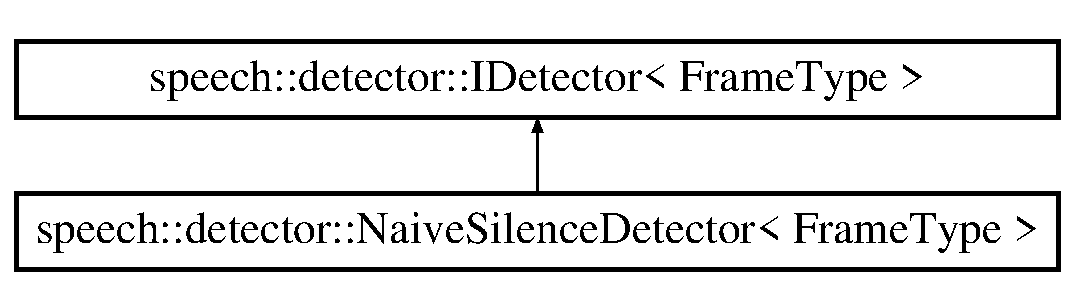
\includegraphics[height=2.000000cm]{classspeech_1_1detector_1_1NaiveSilenceDetector}
\end{center}
\end{figure}
\subsection*{Public Member Functions}
\begin{DoxyCompactItemize}
\item 
virtual bool \hyperlink{classspeech_1_1detector_1_1NaiveSilenceDetector_a5d2bc90b3012c10496b557a96a71aa68}{detected} (\hyperlink{classspeech_1_1raw__data_1_1FrequencySample}{Frequency\+Sample}$<$ Frame\+Type $>$ \&sample) const 
\end{DoxyCompactItemize}


\subsection{Detailed Description}
\subsubsection*{template$<$typename Frame\+Type$>$class speech\+::detector\+::\+Naive\+Silence\+Detector$<$ Frame\+Type $>$}

The detector of silence based on some intuitions only. It checks the mean and standard deviation of the signal amplitude with thresholding. Silence tends to use some high frequencies (noise) and using this intution we try to detect it. 

\subsection{Member Function Documentation}
\hypertarget{classspeech_1_1detector_1_1NaiveSilenceDetector_a5d2bc90b3012c10496b557a96a71aa68}{\index{speech\+::detector\+::\+Naive\+Silence\+Detector@{speech\+::detector\+::\+Naive\+Silence\+Detector}!detected@{detected}}
\index{detected@{detected}!speech\+::detector\+::\+Naive\+Silence\+Detector@{speech\+::detector\+::\+Naive\+Silence\+Detector}}
\subsubsection[{detected}]{\setlength{\rightskip}{0pt plus 5cm}template$<$typename Frame\+Type $>$ bool {\bf speech\+::detector\+::\+Naive\+Silence\+Detector}$<$ Frame\+Type $>$\+::detected (
\begin{DoxyParamCaption}
\item[{{\bf Frequency\+Sample}$<$ Frame\+Type $>$ \&}]{sample}
\end{DoxyParamCaption}
) const\hspace{0.3cm}{\ttfamily [virtual]}}}\label{classspeech_1_1detector_1_1NaiveSilenceDetector_a5d2bc90b3012c10496b557a96a71aa68}
Checks the condition of the particular detector, and returns T\+R\+U\+E if the condition was met, F\+A\+L\+S\+E otherwise.

\begin{DoxyReturn}{Returns}
T\+R\+U\+E -\/ if detected the pattern, F\+A\+L\+S\+E otherwise 
\end{DoxyReturn}


Implements \hyperlink{classspeech_1_1detector_1_1IDetector_a351b24904f920bc42cdcfa1f1c91f479}{speech\+::detector\+::\+I\+Detector$<$ Frame\+Type $>$}.



The documentation for this class was generated from the following files\+:\begin{DoxyCompactItemize}
\item 
/home/kacper/\+Projects/speech-\/recognition/src/speech/detector/Naive\+Silence\+Detector.\+h\item 
/home/kacper/\+Projects/speech-\/recognition/src/speech/detector/Naive\+Silence\+Detector.\+cpp\end{DoxyCompactItemize}

\hypertarget{classspeech_1_1raw__data_1_1DataSource_1_1normalIterator}{\section{speech\+:\+:raw\+\_\+data\+:\+:Data\+Source$<$ Frame\+Type $>$\+:\+:normal\+Iterator Class Reference}
\label{classspeech_1_1raw__data_1_1DataSource_1_1normalIterator}\index{speech\+::raw\+\_\+data\+::\+Data\+Source$<$ Frame\+Type $>$\+::normal\+Iterator@{speech\+::raw\+\_\+data\+::\+Data\+Source$<$ Frame\+Type $>$\+::normal\+Iterator}}
}
Inheritance diagram for speech\+:\+:raw\+\_\+data\+:\+:Data\+Source$<$ Frame\+Type $>$\+:\+:normal\+Iterator\+:\begin{figure}[H]
\begin{center}
\leavevmode
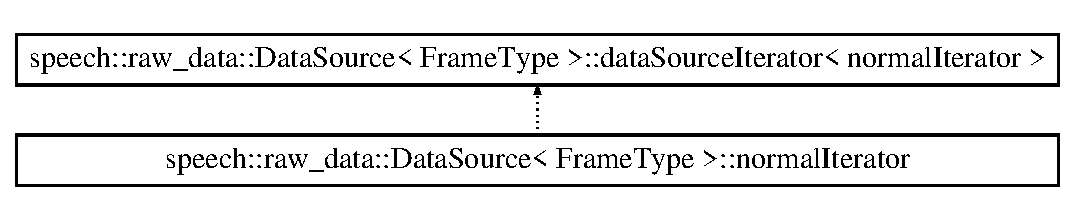
\includegraphics[height=2.000000cm]{classspeech_1_1raw__data_1_1DataSource_1_1normalIterator}
\end{center}
\end{figure}
\subsection*{Public Member Functions}
\begin{DoxyCompactItemize}
\item 
\hypertarget{classspeech_1_1raw__data_1_1DataSource_1_1normalIterator_a1748edb829cff8ee67a5796a0f9b189c}{{\bfseries normal\+Iterator} (typename list$<$ \hyperlink{classspeech_1_1raw__data_1_1DataSample}{Data\+Sample}$<$ Frame\+Type $>$$>$\+::iterator samples\+Iterator)}\label{classspeech_1_1raw__data_1_1DataSource_1_1normalIterator_a1748edb829cff8ee67a5796a0f9b189c}

\item 
\hypertarget{classspeech_1_1raw__data_1_1DataSource_1_1normalIterator_a4fa6120f2a2f58e41800f4132e4086c9}{virtual bool {\bfseries operator==} (const \hyperlink{classspeech_1_1raw__data_1_1DataSource_1_1normalIterator}{normal\+Iterator} \&it)}\label{classspeech_1_1raw__data_1_1DataSource_1_1normalIterator_a4fa6120f2a2f58e41800f4132e4086c9}

\item 
\hypertarget{classspeech_1_1raw__data_1_1DataSource_1_1normalIterator_acf589a04c71c650ab33132771c83f5de}{virtual bool {\bfseries operator!=} (const \hyperlink{classspeech_1_1raw__data_1_1DataSource_1_1normalIterator}{normal\+Iterator} \&it)}\label{classspeech_1_1raw__data_1_1DataSource_1_1normalIterator_acf589a04c71c650ab33132771c83f5de}

\item 
\hypertarget{classspeech_1_1raw__data_1_1DataSource_1_1normalIterator_a34c88d14804e99777ba24284468bb54c}{virtual void {\bfseries operator++} ()}\label{classspeech_1_1raw__data_1_1DataSource_1_1normalIterator_a34c88d14804e99777ba24284468bb54c}

\item 
\hypertarget{classspeech_1_1raw__data_1_1DataSource_1_1normalIterator_a6ec139e8d64ff37cb0995d19dfaff496}{virtual \hyperlink{classspeech_1_1raw__data_1_1DataSample}{Data\+Sample}$<$ Frame\+Type $>$ {\bfseries operator$\ast$} ()}\label{classspeech_1_1raw__data_1_1DataSource_1_1normalIterator_a6ec139e8d64ff37cb0995d19dfaff496}

\end{DoxyCompactItemize}


The documentation for this class was generated from the following file\+:\begin{DoxyCompactItemize}
\item 
/home/kacper/\+Projects/speech-\/recognition/src/speech/raw\+\_\+data/Data\+Source.\+h\end{DoxyCompactItemize}

\hypertarget{classspeech_1_1exception_1_1NullptrSerializationException}{\section{speech\+:\+:exception\+:\+:Nullptr\+Serialization\+Exception Class Reference}
\label{classspeech_1_1exception_1_1NullptrSerializationException}\index{speech\+::exception\+::\+Nullptr\+Serialization\+Exception@{speech\+::exception\+::\+Nullptr\+Serialization\+Exception}}
}
Inheritance diagram for speech\+:\+:exception\+:\+:Nullptr\+Serialization\+Exception\+:\begin{figure}[H]
\begin{center}
\leavevmode
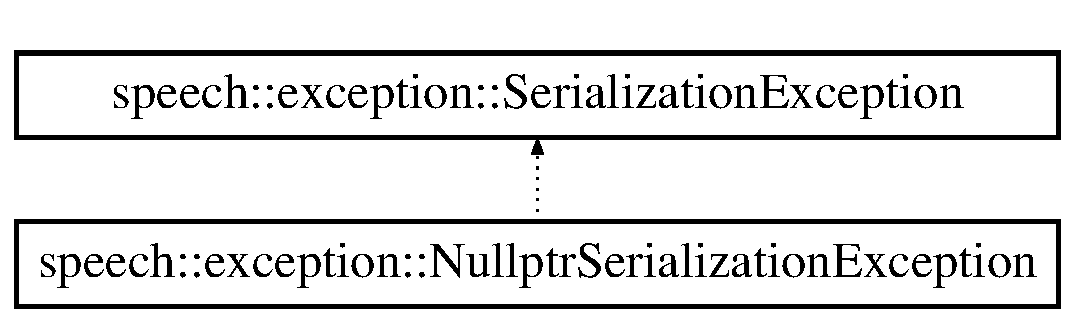
\includegraphics[height=2.000000cm]{classspeech_1_1exception_1_1NullptrSerializationException}
\end{center}
\end{figure}
\subsection*{Public Member Functions}
\begin{DoxyCompactItemize}
\item 
\hypertarget{classspeech_1_1exception_1_1NullptrSerializationException_a959396c385ef4483137e683d26c92649}{{\bfseries Nullptr\+Serialization\+Exception} (const char $\ast$msg)}\label{classspeech_1_1exception_1_1NullptrSerializationException_a959396c385ef4483137e683d26c92649}

\item 
\hypertarget{classspeech_1_1exception_1_1NullptrSerializationException_abd249bbe77755b13a85cf9b415c48a40}{virtual const char $\ast$ {\bfseries what} () const \+\_\+\+G\+L\+I\+B\+C\+X\+X\+\_\+\+U\+S\+E\+\_\+\+N\+O\+E\+X\+C\+E\+P\+T}\label{classspeech_1_1exception_1_1NullptrSerializationException_abd249bbe77755b13a85cf9b415c48a40}

\end{DoxyCompactItemize}


The documentation for this class was generated from the following file\+:\begin{DoxyCompactItemize}
\item 
/home/kacper/\+Projects/speech-\/recognition/src/speech/exception/Nullptr\+Serialization\+Exception.\+h\end{DoxyCompactItemize}

\hypertarget{classspeech_1_1raw__data_1_1DataSource_1_1offsetIterator}{\section{speech\+:\+:raw\+\_\+data\+:\+:Data\+Source$<$ Frame\+Type $>$\+:\+:offset\+Iterator Class Reference}
\label{classspeech_1_1raw__data_1_1DataSource_1_1offsetIterator}\index{speech\+::raw\+\_\+data\+::\+Data\+Source$<$ Frame\+Type $>$\+::offset\+Iterator@{speech\+::raw\+\_\+data\+::\+Data\+Source$<$ Frame\+Type $>$\+::offset\+Iterator}}
}
Inheritance diagram for speech\+:\+:raw\+\_\+data\+:\+:Data\+Source$<$ Frame\+Type $>$\+:\+:offset\+Iterator\+:\begin{figure}[H]
\begin{center}
\leavevmode
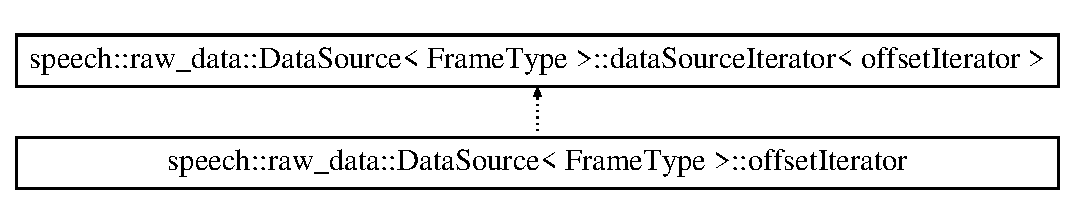
\includegraphics[height=2.000000cm]{classspeech_1_1raw__data_1_1DataSource_1_1offsetIterator}
\end{center}
\end{figure}
\subsection*{Public Member Functions}
\begin{DoxyCompactItemize}
\item 
\hypertarget{classspeech_1_1raw__data_1_1DataSource_1_1offsetIterator_a2cba201886aaa45cc7a71ce294a47491}{virtual bool {\bfseries operator==} (const \hyperlink{classspeech_1_1raw__data_1_1DataSource_1_1offsetIterator}{offset\+Iterator} \&it)}\label{classspeech_1_1raw__data_1_1DataSource_1_1offsetIterator_a2cba201886aaa45cc7a71ce294a47491}

\item 
\hypertarget{classspeech_1_1raw__data_1_1DataSource_1_1offsetIterator_a6f19eda5eed84b836b90a78ac06c8646}{virtual bool {\bfseries operator!=} (const \hyperlink{classspeech_1_1raw__data_1_1DataSource_1_1offsetIterator}{offset\+Iterator} \&it)}\label{classspeech_1_1raw__data_1_1DataSource_1_1offsetIterator_a6f19eda5eed84b836b90a78ac06c8646}

\item 
\hypertarget{classspeech_1_1raw__data_1_1DataSource_1_1offsetIterator_a168b72b3e990f0d13c3be9630d8f5db3}{virtual void {\bfseries operator++} (int)}\label{classspeech_1_1raw__data_1_1DataSource_1_1offsetIterator_a168b72b3e990f0d13c3be9630d8f5db3}

\item 
\hypertarget{classspeech_1_1raw__data_1_1DataSource_1_1offsetIterator_a10edaa7cbd9ac318ac5643f4aa67d758}{virtual void {\bfseries operator++} ()}\label{classspeech_1_1raw__data_1_1DataSource_1_1offsetIterator_a10edaa7cbd9ac318ac5643f4aa67d758}

\item 
\hypertarget{classspeech_1_1raw__data_1_1DataSource_1_1offsetIterator_ae2226d1a53c74574087169b1a2c5ab78}{virtual \hyperlink{classspeech_1_1raw__data_1_1DataSample}{Data\+Sample}$<$ Frame\+Type $>$ {\bfseries operator$\ast$} ()}\label{classspeech_1_1raw__data_1_1DataSource_1_1offsetIterator_ae2226d1a53c74574087169b1a2c5ab78}

\end{DoxyCompactItemize}
\subsection*{Friends}
\begin{DoxyCompactItemize}
\item 
\hypertarget{classspeech_1_1raw__data_1_1DataSource_1_1offsetIterator_a7998ddaa8bd7c3b9a7cd2a8cbf3573c4}{class {\bfseries Data\+Source}}\label{classspeech_1_1raw__data_1_1DataSource_1_1offsetIterator_a7998ddaa8bd7c3b9a7cd2a8cbf3573c4}

\end{DoxyCompactItemize}


The documentation for this class was generated from the following file\+:\begin{DoxyCompactItemize}
\item 
/home/kacper/\+Projects/speech-\/recognition/src/speech/raw\+\_\+data/Data\+Source.\+h\end{DoxyCompactItemize}

\hypertarget{classspeech_1_1initializer_1_1RandomInitializer}{\section{speech\+:\+:initializer\+:\+:Random\+Initializer Class Reference}
\label{classspeech_1_1initializer_1_1RandomInitializer}\index{speech\+::initializer\+::\+Random\+Initializer@{speech\+::initializer\+::\+Random\+Initializer}}
}
Inheritance diagram for speech\+:\+:initializer\+:\+:Random\+Initializer\+:\begin{figure}[H]
\begin{center}
\leavevmode
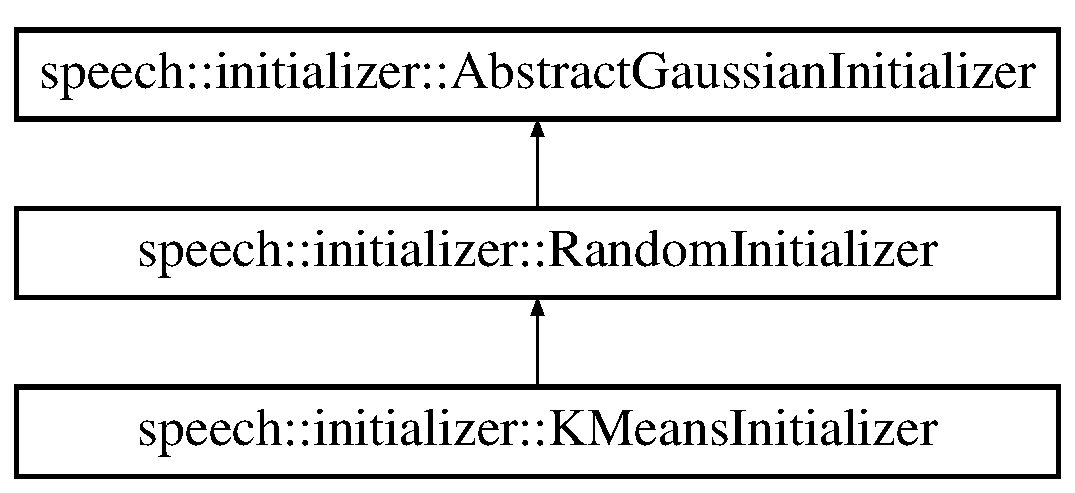
\includegraphics[height=3.000000cm]{classspeech_1_1initializer_1_1RandomInitializer}
\end{center}
\end{figure}
\subsection*{Public Member Functions}
\begin{DoxyCompactItemize}
\item 
virtual void \hyperlink{classspeech_1_1initializer_1_1RandomInitializer_a62c031971e30c4c99516a20268511963}{initialize} (\hyperlink{classspeech_1_1HMMLexicon_1_1MultivariateGaussianHMM}{speech\+::\+H\+M\+M\+Lexicon\+::\+Multivariate\+Gaussian\+H\+M\+M} \&gaussian\+H\+M\+M)
\end{DoxyCompactItemize}
\subsection*{Protected Member Functions}
\begin{DoxyCompactItemize}
\item 
\hypertarget{classspeech_1_1initializer_1_1RandomInitializer_a8c6b73ee9352b17f057064471f5fc10e}{unsigned int {\bfseries count\+Observations} (std\+::vector$<$ H\+M\+M\+Lexicon\+::\+Observation $>$ $\ast$utterances)}\label{classspeech_1_1initializer_1_1RandomInitializer_a8c6b73ee9352b17f057064471f5fc10e}

\item 
\hypertarget{classspeech_1_1initializer_1_1RandomInitializer_a111717598877c98b52fe656fe0e89057}{std\+::valarray$<$ double $>$ {\bfseries calculate\+Mean} (std\+::vector$<$ H\+M\+M\+Lexicon\+::\+Observation $>$ $\ast$utterances, int dimensionality, int observations\+Nb)}\label{classspeech_1_1initializer_1_1RandomInitializer_a111717598877c98b52fe656fe0e89057}

\item 
\hypertarget{classspeech_1_1initializer_1_1RandomInitializer_aad1a53176bb36eeb7d99fd56b9eec5ac}{std\+::valarray$<$ double $>$ {\bfseries calculate\+Variance} (std\+::vector$<$ H\+M\+M\+Lexicon\+::\+Observation $>$ $\ast$utterances, int dimensionality, int observations\+Nb)}\label{classspeech_1_1initializer_1_1RandomInitializer_aad1a53176bb36eeb7d99fd56b9eec5ac}

\end{DoxyCompactItemize}


\subsection{Member Function Documentation}
\hypertarget{classspeech_1_1initializer_1_1RandomInitializer_a62c031971e30c4c99516a20268511963}{\index{speech\+::initializer\+::\+Random\+Initializer@{speech\+::initializer\+::\+Random\+Initializer}!initialize@{initialize}}
\index{initialize@{initialize}!speech\+::initializer\+::\+Random\+Initializer@{speech\+::initializer\+::\+Random\+Initializer}}
\subsubsection[{initialize}]{\setlength{\rightskip}{0pt plus 5cm}void speech\+::initializer\+::\+Random\+Initializer\+::initialize (
\begin{DoxyParamCaption}
\item[{{\bf speech\+::\+H\+M\+M\+Lexicon\+::\+Multivariate\+Gaussian\+H\+M\+M} \&}]{gaussian\+H\+M\+M}
\end{DoxyParamCaption}
)\hspace{0.3cm}{\ttfamily [virtual]}}}\label{classspeech_1_1initializer_1_1RandomInitializer_a62c031971e30c4c99516a20268511963}
Initializes the Gaussians of given H\+M\+M with means and variances 
\begin{DoxyParams}{Parameters}
{\em gaussian\+Hmm} & instance of Gaussian H\+M\+M \\
\hline
\end{DoxyParams}


Implements \hyperlink{classspeech_1_1initializer_1_1AbstractGaussianInitializer_aa32dc879803a574a9bbd04b9f09f9f79}{speech\+::initializer\+::\+Abstract\+Gaussian\+Initializer}.



Reimplemented in \hyperlink{classspeech_1_1initializer_1_1KMeansInitializer_a300e51ef3bca3d566bffb12f2c6f5924}{speech\+::initializer\+::\+K\+Means\+Initializer}.



The documentation for this class was generated from the following files\+:\begin{DoxyCompactItemize}
\item 
/home/kacper/\+Projects/speech-\/recognition/src/speech/initializer/Random\+Initializer.\+h\item 
/home/kacper/\+Projects/speech-\/recognition/src/speech/initializer/Random\+Initializer.\+cpp\end{DoxyCompactItemize}

\hypertarget{classspeech_1_1exception_1_1SerializationException}{\section{speech\+:\+:exception\+:\+:Serialization\+Exception Class Reference}
\label{classspeech_1_1exception_1_1SerializationException}\index{speech\+::exception\+::\+Serialization\+Exception@{speech\+::exception\+::\+Serialization\+Exception}}
}
Inheritance diagram for speech\+:\+:exception\+:\+:Serialization\+Exception\+:\begin{figure}[H]
\begin{center}
\leavevmode
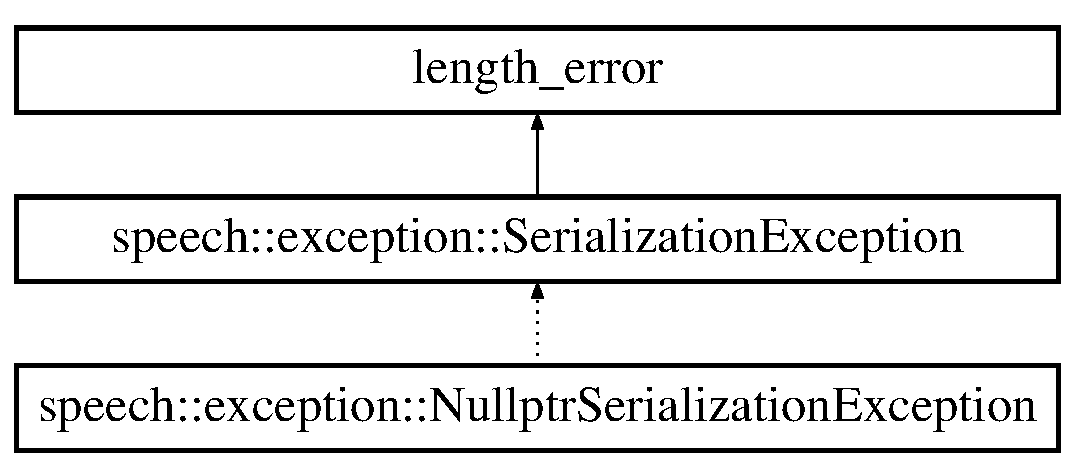
\includegraphics[height=3.000000cm]{classspeech_1_1exception_1_1SerializationException}
\end{center}
\end{figure}
\subsection*{Public Member Functions}
\begin{DoxyCompactItemize}
\item 
\hypertarget{classspeech_1_1exception_1_1SerializationException_ac29c05b9159b68b1096e8574af5fee62}{{\bfseries Serialization\+Exception} (const char $\ast$msg)}\label{classspeech_1_1exception_1_1SerializationException_ac29c05b9159b68b1096e8574af5fee62}

\item 
\hypertarget{classspeech_1_1exception_1_1SerializationException_a8e12d8e8ef2e2864ec677c19fcfbc2e9}{virtual const char $\ast$ {\bfseries what} () const \+\_\+\+G\+L\+I\+B\+C\+X\+X\+\_\+\+U\+S\+E\+\_\+\+N\+O\+E\+X\+C\+E\+P\+T}\label{classspeech_1_1exception_1_1SerializationException_a8e12d8e8ef2e2864ec677c19fcfbc2e9}

\end{DoxyCompactItemize}


The documentation for this class was generated from the following file\+:\begin{DoxyCompactItemize}
\item 
/home/kacper/\+Projects/speech-\/recognition/src/speech/exception/Serialization\+Exception.\+h\end{DoxyCompactItemize}

\hypertarget{classspeech_1_1raw__data_1_1Spectrum}{\section{speech\+:\+:raw\+\_\+data\+:\+:Spectrum Class Reference}
\label{classspeech_1_1raw__data_1_1Spectrum}\index{speech\+::raw\+\_\+data\+::\+Spectrum@{speech\+::raw\+\_\+data\+::\+Spectrum}}
}


{\ttfamily \#include $<$Spectrum.\+h$>$}

\subsection*{Public Member Functions}
\begin{DoxyCompactItemize}
\item 
{\footnotesize template$<$typename Frame\+Type $>$ }\\\hyperlink{classspeech_1_1raw__data_1_1Spectrum_a4a08dc8f79816c923ce2bb27c87ab4cf}{Spectrum} (const \hyperlink{classspeech_1_1raw__data_1_1FrequencySample}{Frequency\+Sample}$<$ Frame\+Type $>$ \&sample)
\item 
virtual \hyperlink{classspeech_1_1raw__data_1_1Spectrum_ac7ad7ef0a8311a2977c2ba3cdbb6af10}{$\sim$\+Spectrum} ()
\item 
std\+::valarray$<$ double $>$ \& \hyperlink{classspeech_1_1raw__data_1_1Spectrum_ace0941220cc60817990d8fbff08e4ba2}{get\+Values} ()
\item 
int \hyperlink{classspeech_1_1raw__data_1_1Spectrum_a32139a1fb7e069a9c906fc2f32b815cf}{get\+Index\+By\+Frequency} (double frequency) const 
\item 
double \hyperlink{classspeech_1_1raw__data_1_1Spectrum_a1833b3262d635ffd6cebd7a8b6ebb0ad}{get\+Index\+Frequency} (int index) const 
\end{DoxyCompactItemize}
\subsection*{Protected Attributes}
\begin{DoxyCompactItemize}
\item 
std\+::valarray$<$ double $>$ \hyperlink{classspeech_1_1raw__data_1_1Spectrum_a8c1ec60def3d84bf834c0fbc3fa44481}{values}
\item 
double \hyperlink{classspeech_1_1raw__data_1_1Spectrum_aa6105ce4e446b344a979dff6980d2d99}{basic\+Frequency}
\end{DoxyCompactItemize}


\subsection{Detailed Description}
\hyperlink{classspeech_1_1raw__data_1_1Spectrum}{Spectrum} of the sound sample 

\subsection{Constructor \& Destructor Documentation}
\hypertarget{classspeech_1_1raw__data_1_1Spectrum_a4a08dc8f79816c923ce2bb27c87ab4cf}{\index{speech\+::raw\+\_\+data\+::\+Spectrum@{speech\+::raw\+\_\+data\+::\+Spectrum}!Spectrum@{Spectrum}}
\index{Spectrum@{Spectrum}!speech\+::raw\+\_\+data\+::\+Spectrum@{speech\+::raw\+\_\+data\+::\+Spectrum}}
\subsubsection[{Spectrum}]{\setlength{\rightskip}{0pt plus 5cm}template$<$typename Frame\+Type $>$ speech\+::raw\+\_\+data\+::\+Spectrum\+::\+Spectrum (
\begin{DoxyParamCaption}
\item[{const {\bf Frequency\+Sample}$<$ Frame\+Type $>$ \&}]{sample}
\end{DoxyParamCaption}
)\hspace{0.3cm}{\ttfamily [inline]}}}\label{classspeech_1_1raw__data_1_1Spectrum_a4a08dc8f79816c923ce2bb27c87ab4cf}
Constructs a spectrum of given sample 
\begin{DoxyParams}{Parameters}
{\em sample} & sound sample in frequency domain \\
\hline
\end{DoxyParams}
\hypertarget{classspeech_1_1raw__data_1_1Spectrum_ac7ad7ef0a8311a2977c2ba3cdbb6af10}{\index{speech\+::raw\+\_\+data\+::\+Spectrum@{speech\+::raw\+\_\+data\+::\+Spectrum}!````~Spectrum@{$\sim$\+Spectrum}}
\index{````~Spectrum@{$\sim$\+Spectrum}!speech\+::raw\+\_\+data\+::\+Spectrum@{speech\+::raw\+\_\+data\+::\+Spectrum}}
\subsubsection[{$\sim$\+Spectrum}]{\setlength{\rightskip}{0pt plus 5cm}virtual speech\+::raw\+\_\+data\+::\+Spectrum\+::$\sim$\+Spectrum (
\begin{DoxyParamCaption}
{}
\end{DoxyParamCaption}
)\hspace{0.3cm}{\ttfamily [inline]}, {\ttfamily [virtual]}}}\label{classspeech_1_1raw__data_1_1Spectrum_ac7ad7ef0a8311a2977c2ba3cdbb6af10}
Destructor 

\subsection{Member Function Documentation}
\hypertarget{classspeech_1_1raw__data_1_1Spectrum_a32139a1fb7e069a9c906fc2f32b815cf}{\index{speech\+::raw\+\_\+data\+::\+Spectrum@{speech\+::raw\+\_\+data\+::\+Spectrum}!get\+Index\+By\+Frequency@{get\+Index\+By\+Frequency}}
\index{get\+Index\+By\+Frequency@{get\+Index\+By\+Frequency}!speech\+::raw\+\_\+data\+::\+Spectrum@{speech\+::raw\+\_\+data\+::\+Spectrum}}
\subsubsection[{get\+Index\+By\+Frequency}]{\setlength{\rightskip}{0pt plus 5cm}int speech\+::raw\+\_\+data\+::\+Spectrum\+::get\+Index\+By\+Frequency (
\begin{DoxyParamCaption}
\item[{double}]{frequency}
\end{DoxyParamCaption}
) const\hspace{0.3cm}{\ttfamily [inline]}}}\label{classspeech_1_1raw__data_1_1Spectrum_a32139a1fb7e069a9c906fc2f32b815cf}
Gets the index of cell containing the value of frequency closest to given frequency 
\begin{DoxyParams}{Parameters}
{\em frequency} & frequency in Herzs \\
\hline
\end{DoxyParams}
\begin{DoxyReturn}{Returns}
index containg this value 
\end{DoxyReturn}
\hypertarget{classspeech_1_1raw__data_1_1Spectrum_a1833b3262d635ffd6cebd7a8b6ebb0ad}{\index{speech\+::raw\+\_\+data\+::\+Spectrum@{speech\+::raw\+\_\+data\+::\+Spectrum}!get\+Index\+Frequency@{get\+Index\+Frequency}}
\index{get\+Index\+Frequency@{get\+Index\+Frequency}!speech\+::raw\+\_\+data\+::\+Spectrum@{speech\+::raw\+\_\+data\+::\+Spectrum}}
\subsubsection[{get\+Index\+Frequency}]{\setlength{\rightskip}{0pt plus 5cm}double speech\+::raw\+\_\+data\+::\+Spectrum\+::get\+Index\+Frequency (
\begin{DoxyParamCaption}
\item[{int}]{index}
\end{DoxyParamCaption}
) const\hspace{0.3cm}{\ttfamily [inline]}}}\label{classspeech_1_1raw__data_1_1Spectrum_a1833b3262d635ffd6cebd7a8b6ebb0ad}
Gets the frequency stored in the given index 
\begin{DoxyParams}{Parameters}
{\em index} & index to check \\
\hline
\end{DoxyParams}
\begin{DoxyReturn}{Returns}
frequency in given index in Herzs 
\end{DoxyReturn}
\hypertarget{classspeech_1_1raw__data_1_1Spectrum_ace0941220cc60817990d8fbff08e4ba2}{\index{speech\+::raw\+\_\+data\+::\+Spectrum@{speech\+::raw\+\_\+data\+::\+Spectrum}!get\+Values@{get\+Values}}
\index{get\+Values@{get\+Values}!speech\+::raw\+\_\+data\+::\+Spectrum@{speech\+::raw\+\_\+data\+::\+Spectrum}}
\subsubsection[{get\+Values}]{\setlength{\rightskip}{0pt plus 5cm}std\+::valarray$<$double$>$\& speech\+::raw\+\_\+data\+::\+Spectrum\+::get\+Values (
\begin{DoxyParamCaption}
{}
\end{DoxyParamCaption}
)\hspace{0.3cm}{\ttfamily [inline]}}}\label{classspeech_1_1raw__data_1_1Spectrum_ace0941220cc60817990d8fbff08e4ba2}
Returns values of the spectrum for given sample \begin{DoxyReturn}{Returns}
spectrum values 
\end{DoxyReturn}


\subsection{Member Data Documentation}
\hypertarget{classspeech_1_1raw__data_1_1Spectrum_aa6105ce4e446b344a979dff6980d2d99}{\index{speech\+::raw\+\_\+data\+::\+Spectrum@{speech\+::raw\+\_\+data\+::\+Spectrum}!basic\+Frequency@{basic\+Frequency}}
\index{basic\+Frequency@{basic\+Frequency}!speech\+::raw\+\_\+data\+::\+Spectrum@{speech\+::raw\+\_\+data\+::\+Spectrum}}
\subsubsection[{basic\+Frequency}]{\setlength{\rightskip}{0pt plus 5cm}double speech\+::raw\+\_\+data\+::\+Spectrum\+::basic\+Frequency\hspace{0.3cm}{\ttfamily [protected]}}}\label{classspeech_1_1raw__data_1_1Spectrum_aa6105ce4e446b344a979dff6980d2d99}
A frequency of the first amplitude \hypertarget{classspeech_1_1raw__data_1_1Spectrum_a8c1ec60def3d84bf834c0fbc3fa44481}{\index{speech\+::raw\+\_\+data\+::\+Spectrum@{speech\+::raw\+\_\+data\+::\+Spectrum}!values@{values}}
\index{values@{values}!speech\+::raw\+\_\+data\+::\+Spectrum@{speech\+::raw\+\_\+data\+::\+Spectrum}}
\subsubsection[{values}]{\setlength{\rightskip}{0pt plus 5cm}std\+::valarray$<$double$>$ speech\+::raw\+\_\+data\+::\+Spectrum\+::values\hspace{0.3cm}{\ttfamily [protected]}}}\label{classspeech_1_1raw__data_1_1Spectrum_a8c1ec60def3d84bf834c0fbc3fa44481}
Squared magnitude (amplitude) of given sample 

The documentation for this class was generated from the following file\+:\begin{DoxyCompactItemize}
\item 
/home/kacper/\+Projects/speech-\/recognition/src/speech/raw\+\_\+data/Spectrum.\+h\end{DoxyCompactItemize}

\hypertarget{classspeech_1_1spelling_1_1SpellingAdjuster}{\section{speech\+:\+:spelling\+:\+:Spelling\+Adjuster Class Reference}
\label{classspeech_1_1spelling_1_1SpellingAdjuster}\index{speech\+::spelling\+::\+Spelling\+Adjuster@{speech\+::spelling\+::\+Spelling\+Adjuster}}
}


{\ttfamily \#include $<$Spelling\+Adjuster.\+h$>$}

\subsection*{Public Member Functions}
\begin{DoxyCompactItemize}
\item 
\hypertarget{classspeech_1_1spelling_1_1SpellingAdjuster_af4a4c7a1aa754a5a0c4bf1a1019edc66}{std\+::string {\bfseries adjust} (const std\+::string \&text, const int length)}\label{classspeech_1_1spelling_1_1SpellingAdjuster_af4a4c7a1aa754a5a0c4bf1a1019edc66}

\end{DoxyCompactItemize}


\subsection{Detailed Description}
This class performs an adjustment of the length of given word by duplicating the letters. It is done using the language model (some letters last longer than another ones). 

The documentation for this class was generated from the following files\+:\begin{DoxyCompactItemize}
\item 
/home/kacper/\+Projects/speech-\/recognition/src/speech/spelling/Spelling\+Adjuster.\+h\item 
/home/kacper/\+Projects/speech-\/recognition/src/speech/spelling/Spelling\+Adjuster.\+cpp\end{DoxyCompactItemize}

\hypertarget{classspeech_1_1vectorizer_1_1ThirdsPowerVectorizer}{\section{speech\+:\+:vectorizer\+:\+:Thirds\+Power\+Vectorizer$<$ Frame\+Type $>$ Class Template Reference}
\label{classspeech_1_1vectorizer_1_1ThirdsPowerVectorizer}\index{speech\+::vectorizer\+::\+Thirds\+Power\+Vectorizer$<$ Frame\+Type $>$@{speech\+::vectorizer\+::\+Thirds\+Power\+Vectorizer$<$ Frame\+Type $>$}}
}
Inheritance diagram for speech\+:\+:vectorizer\+:\+:Thirds\+Power\+Vectorizer$<$ Frame\+Type $>$\+:\begin{figure}[H]
\begin{center}
\leavevmode
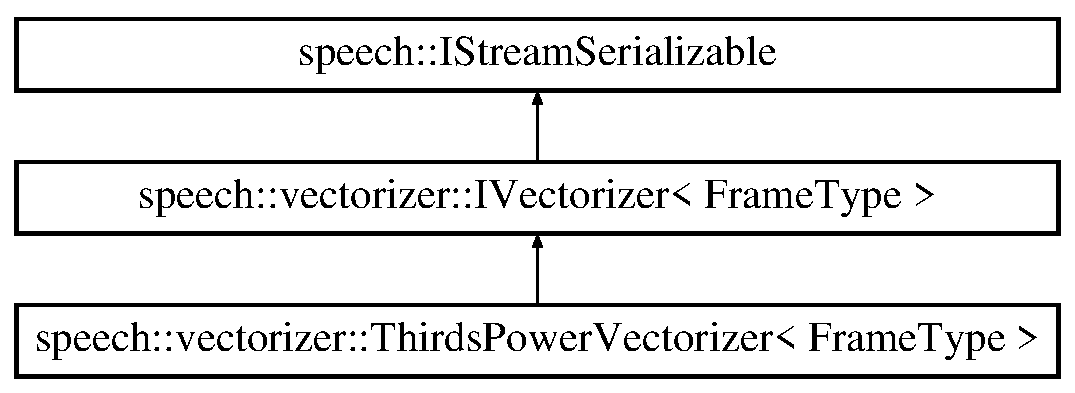
\includegraphics[height=3.000000cm]{classspeech_1_1vectorizer_1_1ThirdsPowerVectorizer}
\end{center}
\end{figure}
\subsection*{Public Member Functions}
\begin{DoxyCompactItemize}
\item 
\hypertarget{classspeech_1_1vectorizer_1_1ThirdsPowerVectorizer_a44431bd02c11d430a2206bcf4950008b}{{\bfseries Thirds\+Power\+Vectorizer} (std\+::istream \&istream)}\label{classspeech_1_1vectorizer_1_1ThirdsPowerVectorizer_a44431bd02c11d430a2206bcf4950008b}

\item 
virtual std\+::valarray$<$ double $>$ \hyperlink{classspeech_1_1vectorizer_1_1ThirdsPowerVectorizer_aa43af654f25abdb9a1698815edaf900c}{vectorize} (\hyperlink{classspeech_1_1raw__data_1_1FrequencySample}{Frequency\+Sample}$<$ Frame\+Type $>$ \&sample)
\item 
virtual void \hyperlink{classspeech_1_1vectorizer_1_1ThirdsPowerVectorizer_ab27c49171171fa2af908d9f3df0712db}{serialize} (std\+::ostream \&out) const 
\item 
virtual int \hyperlink{classspeech_1_1vectorizer_1_1ThirdsPowerVectorizer_a4680e178d5ef376cf2e4f6d47487e047}{get\+Vector\+Size} () const 
\end{DoxyCompactItemize}
\subsection*{Static Public Attributes}
\begin{DoxyCompactItemize}
\item 
\hypertarget{classspeech_1_1vectorizer_1_1ThirdsPowerVectorizer_a1390e6e6e099b5f573ec1f47b5d76f76}{static const uint32\+\_\+t {\bfseries T\+Y\+P\+E\+\_\+\+I\+D\+E\+N\+T\+I\+F\+I\+E\+R} = 0x00100003}\label{classspeech_1_1vectorizer_1_1ThirdsPowerVectorizer_a1390e6e6e099b5f573ec1f47b5d76f76}

\end{DoxyCompactItemize}
\subsection*{Protected Member Functions}
\begin{DoxyCompactItemize}
\item 
double \hyperlink{classspeech_1_1vectorizer_1_1ThirdsPowerVectorizer_acf6519f34d3bd003d09a62ae0b42fcb9}{get\+Third\+Energy} (double $\ast$amplitude\+Ptr, int lower\+Index, int upper\+Index)
\end{DoxyCompactItemize}
\subsection*{Additional Inherited Members}


\subsection{Member Function Documentation}
\hypertarget{classspeech_1_1vectorizer_1_1ThirdsPowerVectorizer_acf6519f34d3bd003d09a62ae0b42fcb9}{\index{speech\+::vectorizer\+::\+Thirds\+Power\+Vectorizer@{speech\+::vectorizer\+::\+Thirds\+Power\+Vectorizer}!get\+Third\+Energy@{get\+Third\+Energy}}
\index{get\+Third\+Energy@{get\+Third\+Energy}!speech\+::vectorizer\+::\+Thirds\+Power\+Vectorizer@{speech\+::vectorizer\+::\+Thirds\+Power\+Vectorizer}}
\subsubsection[{get\+Third\+Energy}]{\setlength{\rightskip}{0pt plus 5cm}template$<$typename Frame\+Type $>$ double {\bf speech\+::vectorizer\+::\+Thirds\+Power\+Vectorizer}$<$ Frame\+Type $>$\+::get\+Third\+Energy (
\begin{DoxyParamCaption}
\item[{double $\ast$}]{amplitude\+Ptr, }
\item[{int}]{lower\+Index, }
\item[{int}]{upper\+Index}
\end{DoxyParamCaption}
)\hspace{0.3cm}{\ttfamily [protected]}}}\label{classspeech_1_1vectorizer_1_1ThirdsPowerVectorizer_acf6519f34d3bd003d09a62ae0b42fcb9}
Calculates an average energy of the third hidden behind given indexes \begin{DoxyReturn}{Returns}
double 
\end{DoxyReturn}
\hypertarget{classspeech_1_1vectorizer_1_1ThirdsPowerVectorizer_a4680e178d5ef376cf2e4f6d47487e047}{\index{speech\+::vectorizer\+::\+Thirds\+Power\+Vectorizer@{speech\+::vectorizer\+::\+Thirds\+Power\+Vectorizer}!get\+Vector\+Size@{get\+Vector\+Size}}
\index{get\+Vector\+Size@{get\+Vector\+Size}!speech\+::vectorizer\+::\+Thirds\+Power\+Vectorizer@{speech\+::vectorizer\+::\+Thirds\+Power\+Vectorizer}}
\subsubsection[{get\+Vector\+Size}]{\setlength{\rightskip}{0pt plus 5cm}template$<$typename Frame\+Type $>$ int {\bf speech\+::vectorizer\+::\+Thirds\+Power\+Vectorizer}$<$ Frame\+Type $>$\+::get\+Vector\+Size (
\begin{DoxyParamCaption}
{}
\end{DoxyParamCaption}
) const\hspace{0.3cm}{\ttfamily [virtual]}}}\label{classspeech_1_1vectorizer_1_1ThirdsPowerVectorizer_a4680e178d5ef376cf2e4f6d47487e047}
Gets the size of the output vector produced by the vectorizer.

\begin{DoxyReturn}{Returns}
size of the produced vector 
\end{DoxyReturn}


Implements \hyperlink{classspeech_1_1vectorizer_1_1IVectorizer_abe20529a1586c072783f42476ad7ab69}{speech\+::vectorizer\+::\+I\+Vectorizer$<$ Frame\+Type $>$}.

\hypertarget{classspeech_1_1vectorizer_1_1ThirdsPowerVectorizer_ab27c49171171fa2af908d9f3df0712db}{\index{speech\+::vectorizer\+::\+Thirds\+Power\+Vectorizer@{speech\+::vectorizer\+::\+Thirds\+Power\+Vectorizer}!serialize@{serialize}}
\index{serialize@{serialize}!speech\+::vectorizer\+::\+Thirds\+Power\+Vectorizer@{speech\+::vectorizer\+::\+Thirds\+Power\+Vectorizer}}
\subsubsection[{serialize}]{\setlength{\rightskip}{0pt plus 5cm}template$<$typename Frame\+Type $>$ void {\bf speech\+::vectorizer\+::\+Thirds\+Power\+Vectorizer}$<$ Frame\+Type $>$\+::serialize (
\begin{DoxyParamCaption}
\item[{std\+::ostream \&}]{out}
\end{DoxyParamCaption}
) const\hspace{0.3cm}{\ttfamily [virtual]}}}\label{classspeech_1_1vectorizer_1_1ThirdsPowerVectorizer_ab27c49171171fa2af908d9f3df0712db}
Serializes the vectorizer into given stream. 
\begin{DoxyParams}{Parameters}
{\em out} & output stream \\
\hline
\end{DoxyParams}


Implements \hyperlink{classspeech_1_1vectorizer_1_1IVectorizer_aa8285bbd275c31ae1ce48d294400dea9}{speech\+::vectorizer\+::\+I\+Vectorizer$<$ Frame\+Type $>$}.

\hypertarget{classspeech_1_1vectorizer_1_1ThirdsPowerVectorizer_aa43af654f25abdb9a1698815edaf900c}{\index{speech\+::vectorizer\+::\+Thirds\+Power\+Vectorizer@{speech\+::vectorizer\+::\+Thirds\+Power\+Vectorizer}!vectorize@{vectorize}}
\index{vectorize@{vectorize}!speech\+::vectorizer\+::\+Thirds\+Power\+Vectorizer@{speech\+::vectorizer\+::\+Thirds\+Power\+Vectorizer}}
\subsubsection[{vectorize}]{\setlength{\rightskip}{0pt plus 5cm}template$<$typename Frame\+Type $>$ std\+::valarray$<$ double $>$ {\bf speech\+::vectorizer\+::\+Thirds\+Power\+Vectorizer}$<$ Frame\+Type $>$\+::vectorize (
\begin{DoxyParamCaption}
\item[{{\bf Frequency\+Sample}$<$ Frame\+Type $>$ \&}]{sample}
\end{DoxyParamCaption}
)\hspace{0.3cm}{\ttfamily [virtual]}}}\label{classspeech_1_1vectorizer_1_1ThirdsPowerVectorizer_aa43af654f25abdb9a1698815edaf900c}
Projects given sample into feature space. Each vector needs to have exactly same size. 
\begin{DoxyParams}{Parameters}
{\em sample} & single sample to be vectorized\\
\hline
\end{DoxyParams}
\begin{DoxyReturn}{Returns}
the projection of vector in a feature space 
\end{DoxyReturn}


Implements \hyperlink{classspeech_1_1vectorizer_1_1IVectorizer_a00d2ba71ec5c447780ffb0a29bfc9085}{speech\+::vectorizer\+::\+I\+Vectorizer$<$ Frame\+Type $>$}.



The documentation for this class was generated from the following files\+:\begin{DoxyCompactItemize}
\item 
/home/kacper/\+Projects/speech-\/recognition/src/speech/vectorizer/Thirds\+Power\+Vectorizer.\+h\item 
/home/kacper/\+Projects/speech-\/recognition/src/speech/vectorizer/Thirds\+Power\+Vectorizer.\+cpp\end{DoxyCompactItemize}

\hypertarget{classspeech_1_1clustering_1_1exception_1_1TooLessVectorsException}{\section{speech\+:\+:clustering\+:\+:exception\+:\+:Too\+Less\+Vectors\+Exception Class Reference}
\label{classspeech_1_1clustering_1_1exception_1_1TooLessVectorsException}\index{speech\+::clustering\+::exception\+::\+Too\+Less\+Vectors\+Exception@{speech\+::clustering\+::exception\+::\+Too\+Less\+Vectors\+Exception}}
}
Inheritance diagram for speech\+:\+:clustering\+:\+:exception\+:\+:Too\+Less\+Vectors\+Exception\+:\begin{figure}[H]
\begin{center}
\leavevmode
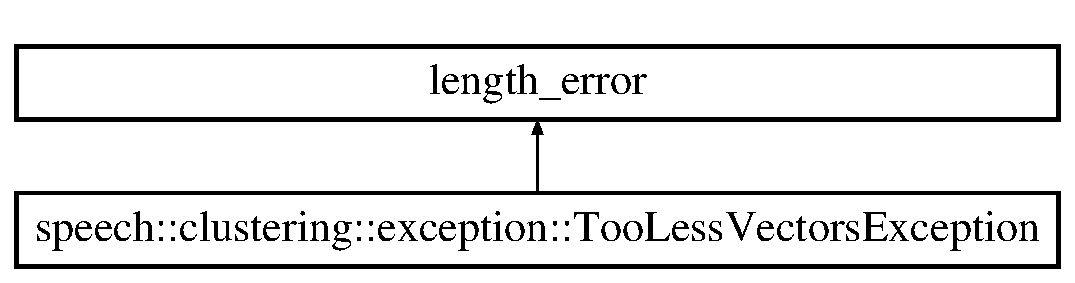
\includegraphics[height=2.000000cm]{classspeech_1_1clustering_1_1exception_1_1TooLessVectorsException}
\end{center}
\end{figure}


The documentation for this class was generated from the following file\+:\begin{DoxyCompactItemize}
\item 
/home/kacper/\+Projects/speech-\/recognition/src/speech/clustering/exception/Too\+Less\+Vectors\+Exception.\+h\end{DoxyCompactItemize}

\hypertarget{structspeech_1_1raw__data_1_1wav__header}{\section{speech\+:\+:raw\+\_\+data\+:\+:wav\+\_\+header Struct Reference}
\label{structspeech_1_1raw__data_1_1wav__header}\index{speech\+::raw\+\_\+data\+::wav\+\_\+header@{speech\+::raw\+\_\+data\+::wav\+\_\+header}}
}
\subsection*{Public Attributes}
\begin{DoxyCompactItemize}
\item 
\hypertarget{structspeech_1_1raw__data_1_1wav__header_aa21e9d3717f09b9fdb6858d63ce07536}{char {\bfseries chunk\+\_\+id} \mbox{[}4\mbox{]}}\label{structspeech_1_1raw__data_1_1wav__header_aa21e9d3717f09b9fdb6858d63ce07536}

\item 
\hypertarget{structspeech_1_1raw__data_1_1wav__header_a547c4d3fda743ec9357740a575ec2422}{int {\bfseries chunk\+\_\+size}}\label{structspeech_1_1raw__data_1_1wav__header_a547c4d3fda743ec9357740a575ec2422}

\item 
\hypertarget{structspeech_1_1raw__data_1_1wav__header_aed4df24a7d029bda68a4944971eed1c2}{char {\bfseries format} \mbox{[}4\mbox{]}}\label{structspeech_1_1raw__data_1_1wav__header_aed4df24a7d029bda68a4944971eed1c2}

\item 
\hypertarget{structspeech_1_1raw__data_1_1wav__header_a0d8b3070e3abf0c04feecbe9109abe9e}{char {\bfseries subchunk1\+\_\+id} \mbox{[}4\mbox{]}}\label{structspeech_1_1raw__data_1_1wav__header_a0d8b3070e3abf0c04feecbe9109abe9e}

\item 
\hypertarget{structspeech_1_1raw__data_1_1wav__header_ae64a9825c689d3095688dca5915cdef5}{int {\bfseries subchunk1\+\_\+size}}\label{structspeech_1_1raw__data_1_1wav__header_ae64a9825c689d3095688dca5915cdef5}

\item 
\hypertarget{structspeech_1_1raw__data_1_1wav__header_a0c59f8f100613ba4ff6895f4564fae4f}{short int {\bfseries audio\+\_\+format}}\label{structspeech_1_1raw__data_1_1wav__header_a0c59f8f100613ba4ff6895f4564fae4f}

\item 
\hypertarget{structspeech_1_1raw__data_1_1wav__header_ae7fd75d94da1ba6e13f75f1b8a28fe72}{short int {\bfseries num\+\_\+channels}}\label{structspeech_1_1raw__data_1_1wav__header_ae7fd75d94da1ba6e13f75f1b8a28fe72}

\item 
\hypertarget{structspeech_1_1raw__data_1_1wav__header_a4aa3ed860c58f9f4021f2037c727992d}{int {\bfseries sample\+\_\+rate}}\label{structspeech_1_1raw__data_1_1wav__header_a4aa3ed860c58f9f4021f2037c727992d}

\item 
\hypertarget{structspeech_1_1raw__data_1_1wav__header_aff9c077868fcd513113c02928af0adef}{int {\bfseries byte\+\_\+rate}}\label{structspeech_1_1raw__data_1_1wav__header_aff9c077868fcd513113c02928af0adef}

\item 
\hypertarget{structspeech_1_1raw__data_1_1wav__header_aeebff7bdfe06c541bd49a7f2374c3d9d}{short int {\bfseries block\+\_\+align}}\label{structspeech_1_1raw__data_1_1wav__header_aeebff7bdfe06c541bd49a7f2374c3d9d}

\item 
\hypertarget{structspeech_1_1raw__data_1_1wav__header_a01a36c4ec5be08ff14472ab2bb8dcc92}{short int {\bfseries bits\+\_\+per\+\_\+sample}}\label{structspeech_1_1raw__data_1_1wav__header_a01a36c4ec5be08ff14472ab2bb8dcc92}

\item 
\hypertarget{structspeech_1_1raw__data_1_1wav__header_a4179f63d378c3b5e0796922ad6399a07}{char {\bfseries subchunk2\+\_\+id} \mbox{[}4\mbox{]}}\label{structspeech_1_1raw__data_1_1wav__header_a4179f63d378c3b5e0796922ad6399a07}

\item 
\hypertarget{structspeech_1_1raw__data_1_1wav__header_ab87a9319411457322b16134174d77545}{int {\bfseries subchunk2\+\_\+size}}\label{structspeech_1_1raw__data_1_1wav__header_ab87a9319411457322b16134174d77545}

\end{DoxyCompactItemize}


The documentation for this struct was generated from the following file\+:\begin{DoxyCompactItemize}
\item 
/home/kacper/\+Projects/speech-\/recognition/src/speech/raw\+\_\+data/Wave\+File\+Data\+Source.\+h\end{DoxyCompactItemize}

\hypertarget{classspeech_1_1raw__data_1_1WaveFileDataSource}{\section{speech\+:\+:raw\+\_\+data\+:\+:Wave\+File\+Data\+Source$<$ Frame\+Type $>$ Class Template Reference}
\label{classspeech_1_1raw__data_1_1WaveFileDataSource}\index{speech\+::raw\+\_\+data\+::\+Wave\+File\+Data\+Source$<$ Frame\+Type $>$@{speech\+::raw\+\_\+data\+::\+Wave\+File\+Data\+Source$<$ Frame\+Type $>$}}
}


{\ttfamily \#include $<$Wave\+File\+Data\+Source.\+h$>$}

Inheritance diagram for speech\+:\+:raw\+\_\+data\+:\+:Wave\+File\+Data\+Source$<$ Frame\+Type $>$\+:\begin{figure}[H]
\begin{center}
\leavevmode
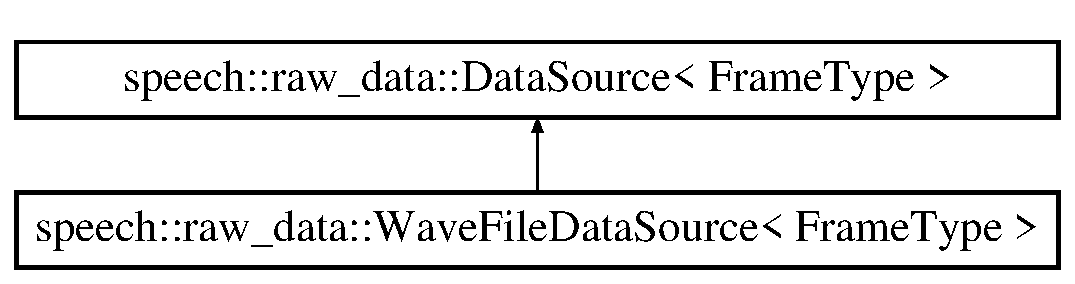
\includegraphics[height=2.000000cm]{classspeech_1_1raw__data_1_1WaveFileDataSource}
\end{center}
\end{figure}
\subsection*{Public Member Functions}
\begin{DoxyCompactItemize}
\item 
\hyperlink{classspeech_1_1raw__data_1_1WaveFileDataSource_a9e8c4f283e57e77fbfb7d8e4c8112d92}{Wave\+File\+Data\+Source} (\hyperlink{structspeech_1_1raw__data_1_1wav__header}{wav\+\_\+header} \+\_\+meta\+\_\+data, int \hyperlink{classspeech_1_1raw__data_1_1DataSource_a6041f72109ebba9e84e49d71f626b8ea}{sample\+Length})
\item 
\hyperlink{classspeech_1_1raw__data_1_1WaveFileDataSource_afd6dc224baa81131e0b09c18ecd42b07}{Wave\+File\+Data\+Source} (string \+\_\+file\+Name, int \hyperlink{classspeech_1_1raw__data_1_1DataSource_a6041f72109ebba9e84e49d71f626b8ea}{sample\+Length})
\item 
virtual \hyperlink{classspeech_1_1raw__data_1_1WaveFileDataSource_ace75bc6dfeb280651d4eaba46edfa922}{$\sim$\+Wave\+File\+Data\+Source} ()
\item 
\hypertarget{classspeech_1_1raw__data_1_1WaveFileDataSource_a62e606a02c1c1068c39cf56979d5943f}{void {\bfseries save\+To\+File} (string \+\_\+file\+Name)}\label{classspeech_1_1raw__data_1_1WaveFileDataSource_a62e606a02c1c1068c39cf56979d5943f}

\item 
\hypertarget{classspeech_1_1raw__data_1_1WaveFileDataSource_a2dca62bfd4d14b853400269a70d5dd0d}{virtual \hyperlink{structspeech_1_1raw__data_1_1wav__header}{wav\+\_\+header} {\bfseries get\+Meta\+Data} ()}\label{classspeech_1_1raw__data_1_1WaveFileDataSource_a2dca62bfd4d14b853400269a70d5dd0d}

\item 
\hypertarget{classspeech_1_1raw__data_1_1WaveFileDataSource_aa89989745215224ceda8c39fe23d6751}{virtual void {\bfseries add\+Sample} (\hyperlink{classspeech_1_1raw__data_1_1DataSample}{Data\+Sample}$<$ Frame\+Type $>$ sample)}\label{classspeech_1_1raw__data_1_1WaveFileDataSource_aa89989745215224ceda8c39fe23d6751}

\item 
\hypertarget{classspeech_1_1raw__data_1_1WaveFileDataSource_a79006acac0a4e1136ef140802e1c2c4d}{virtual void {\bfseries init} ()}\label{classspeech_1_1raw__data_1_1WaveFileDataSource_a79006acac0a4e1136ef140802e1c2c4d}

\end{DoxyCompactItemize}
\subsection*{Static Public Member Functions}
\begin{DoxyCompactItemize}
\item 
static \hyperlink{structspeech_1_1raw__data_1_1wav__header}{wav\+\_\+header} \hyperlink{classspeech_1_1raw__data_1_1WaveFileDataSource_a473179ee3ccc9999017c87928df2a3a6}{create\+Pcm\+Wav\+Header} (short num\+Channels, int sample\+Rate, short bits\+Per\+Sample)
\end{DoxyCompactItemize}
\subsection*{Protected Member Functions}
\begin{DoxyCompactItemize}
\item 
virtual unsigned int \hyperlink{classspeech_1_1raw__data_1_1WaveFileDataSource_ac88d8d6a4d6c1f5cf9031fc4d3153542}{get\+Data\+Sample\+Size} (int size\+In\+Milliseconds)
\item 
virtual unsigned int \hyperlink{classspeech_1_1raw__data_1_1WaveFileDataSource_a62bdc52d91ffeb282da46d42ad3d230c}{get\+Data\+Sample\+Length\+In\+Milliseconds} (int size)
\end{DoxyCompactItemize}
\subsection*{Protected Attributes}
\begin{DoxyCompactItemize}
\item 
string \hyperlink{classspeech_1_1raw__data_1_1WaveFileDataSource_a28870da18426c9339b8f67eec21000be}{file\+Name}
\end{DoxyCompactItemize}


\subsection{Detailed Description}
\subsubsection*{template$<$typename Frame\+Type$>$class speech\+::raw\+\_\+data\+::\+Wave\+File\+Data\+Source$<$ Frame\+Type $>$}

This class represents the data source which reads the signal from standard W\+A\+V file 

\subsection{Constructor \& Destructor Documentation}
\hypertarget{classspeech_1_1raw__data_1_1WaveFileDataSource_a9e8c4f283e57e77fbfb7d8e4c8112d92}{\index{speech\+::raw\+\_\+data\+::\+Wave\+File\+Data\+Source@{speech\+::raw\+\_\+data\+::\+Wave\+File\+Data\+Source}!Wave\+File\+Data\+Source@{Wave\+File\+Data\+Source}}
\index{Wave\+File\+Data\+Source@{Wave\+File\+Data\+Source}!speech\+::raw\+\_\+data\+::\+Wave\+File\+Data\+Source@{speech\+::raw\+\_\+data\+::\+Wave\+File\+Data\+Source}}
\subsubsection[{Wave\+File\+Data\+Source}]{\setlength{\rightskip}{0pt plus 5cm}template$<$typename Frame\+Type $>$ {\bf speech\+::raw\+\_\+data\+::\+Wave\+File\+Data\+Source}$<$ Frame\+Type $>$\+::{\bf Wave\+File\+Data\+Source} (
\begin{DoxyParamCaption}
\item[{{\bf wav\+\_\+header}}]{\+\_\+meta\+\_\+data, }
\item[{int}]{sample\+Length}
\end{DoxyParamCaption}
)}}\label{classspeech_1_1raw__data_1_1WaveFileDataSource_a9e8c4f283e57e77fbfb7d8e4c8112d92}
Construct an empty file with given W\+A\+V file header and length of one \hyperlink{classspeech_1_1raw__data_1_1DataSample}{Data\+Sample} used in sampling.


\begin{DoxyParams}{Parameters}
{\em \+\_\+meta\+\_\+data} & W\+A\+V file header \\
\hline
{\em sample\+Length} & length of a single sample in milliseconds \\
\hline
\end{DoxyParams}
\hypertarget{classspeech_1_1raw__data_1_1WaveFileDataSource_afd6dc224baa81131e0b09c18ecd42b07}{\index{speech\+::raw\+\_\+data\+::\+Wave\+File\+Data\+Source@{speech\+::raw\+\_\+data\+::\+Wave\+File\+Data\+Source}!Wave\+File\+Data\+Source@{Wave\+File\+Data\+Source}}
\index{Wave\+File\+Data\+Source@{Wave\+File\+Data\+Source}!speech\+::raw\+\_\+data\+::\+Wave\+File\+Data\+Source@{speech\+::raw\+\_\+data\+::\+Wave\+File\+Data\+Source}}
\subsubsection[{Wave\+File\+Data\+Source}]{\setlength{\rightskip}{0pt plus 5cm}template$<$typename Frame\+Type $>$ {\bf speech\+::raw\+\_\+data\+::\+Wave\+File\+Data\+Source}$<$ Frame\+Type $>$\+::{\bf Wave\+File\+Data\+Source} (
\begin{DoxyParamCaption}
\item[{string}]{\+\_\+file\+Name, }
\item[{int}]{sample\+Length}
\end{DoxyParamCaption}
)}}\label{classspeech_1_1raw__data_1_1WaveFileDataSource_afd6dc224baa81131e0b09c18ecd42b07}
Construct a file using a file from provided path and length of one \hyperlink{classspeech_1_1raw__data_1_1DataSample}{Data\+Sample} used in sampling.


\begin{DoxyParams}{Parameters}
{\em \+\_\+file\+Name} & path to W\+A\+V file \\
\hline
{\em sample\+Length} & length of a single sample in milliseconds \\
\hline
\end{DoxyParams}
\hypertarget{classspeech_1_1raw__data_1_1WaveFileDataSource_ace75bc6dfeb280651d4eaba46edfa922}{\index{speech\+::raw\+\_\+data\+::\+Wave\+File\+Data\+Source@{speech\+::raw\+\_\+data\+::\+Wave\+File\+Data\+Source}!````~Wave\+File\+Data\+Source@{$\sim$\+Wave\+File\+Data\+Source}}
\index{````~Wave\+File\+Data\+Source@{$\sim$\+Wave\+File\+Data\+Source}!speech\+::raw\+\_\+data\+::\+Wave\+File\+Data\+Source@{speech\+::raw\+\_\+data\+::\+Wave\+File\+Data\+Source}}
\subsubsection[{$\sim$\+Wave\+File\+Data\+Source}]{\setlength{\rightskip}{0pt plus 5cm}template$<$typename Frame\+Type $>$ {\bf speech\+::raw\+\_\+data\+::\+Wave\+File\+Data\+Source}$<$ Frame\+Type $>$\+::$\sim${\bf Wave\+File\+Data\+Source} (
\begin{DoxyParamCaption}
{}
\end{DoxyParamCaption}
)\hspace{0.3cm}{\ttfamily [virtual]}}}\label{classspeech_1_1raw__data_1_1WaveFileDataSource_ace75bc6dfeb280651d4eaba46edfa922}
Destructor 

\subsection{Member Function Documentation}
\hypertarget{classspeech_1_1raw__data_1_1WaveFileDataSource_a473179ee3ccc9999017c87928df2a3a6}{\index{speech\+::raw\+\_\+data\+::\+Wave\+File\+Data\+Source@{speech\+::raw\+\_\+data\+::\+Wave\+File\+Data\+Source}!create\+Pcm\+Wav\+Header@{create\+Pcm\+Wav\+Header}}
\index{create\+Pcm\+Wav\+Header@{create\+Pcm\+Wav\+Header}!speech\+::raw\+\_\+data\+::\+Wave\+File\+Data\+Source@{speech\+::raw\+\_\+data\+::\+Wave\+File\+Data\+Source}}
\subsubsection[{create\+Pcm\+Wav\+Header}]{\setlength{\rightskip}{0pt plus 5cm}template$<$typename Frame\+Type $>$ {\bf speech\+::raw\+\_\+data\+::wav\+\_\+header} {\bf speech\+::raw\+\_\+data\+::\+Wave\+File\+Data\+Source}$<$ Frame\+Type $>$\+::create\+Pcm\+Wav\+Header (
\begin{DoxyParamCaption}
\item[{short}]{num\+Channels, }
\item[{int}]{sample\+Rate, }
\item[{short}]{bits\+Per\+Sample}
\end{DoxyParamCaption}
)\hspace{0.3cm}{\ttfamily [static]}}}\label{classspeech_1_1raw__data_1_1WaveFileDataSource_a473179ee3ccc9999017c87928df2a3a6}
Creates wave header representing pcm wave file with empty data.


\begin{DoxyParams}{Parameters}
{\em num\+Channels} & \\
\hline
{\em sample\+Rate} & \\
\hline
{\em bits\+Per\+Sample} & \\
\hline
\end{DoxyParams}
\hypertarget{classspeech_1_1raw__data_1_1WaveFileDataSource_a62bdc52d91ffeb282da46d42ad3d230c}{\index{speech\+::raw\+\_\+data\+::\+Wave\+File\+Data\+Source@{speech\+::raw\+\_\+data\+::\+Wave\+File\+Data\+Source}!get\+Data\+Sample\+Length\+In\+Milliseconds@{get\+Data\+Sample\+Length\+In\+Milliseconds}}
\index{get\+Data\+Sample\+Length\+In\+Milliseconds@{get\+Data\+Sample\+Length\+In\+Milliseconds}!speech\+::raw\+\_\+data\+::\+Wave\+File\+Data\+Source@{speech\+::raw\+\_\+data\+::\+Wave\+File\+Data\+Source}}
\subsubsection[{get\+Data\+Sample\+Length\+In\+Milliseconds}]{\setlength{\rightskip}{0pt plus 5cm}template$<$typename Frame\+Type $>$ unsigned int {\bf speech\+::raw\+\_\+data\+::\+Wave\+File\+Data\+Source}$<$ Frame\+Type $>$\+::get\+Data\+Sample\+Length\+In\+Milliseconds (
\begin{DoxyParamCaption}
\item[{int}]{size}
\end{DoxyParamCaption}
)\hspace{0.3cm}{\ttfamily [protected]}, {\ttfamily [virtual]}}}\label{classspeech_1_1raw__data_1_1WaveFileDataSource_a62bdc52d91ffeb282da46d42ad3d230c}
Returns length of sample with size 'size'. 

Implements \hyperlink{classspeech_1_1raw__data_1_1DataSource_aa4157ef95d70d9c1babd2e9ead0d573a}{speech\+::raw\+\_\+data\+::\+Data\+Source$<$ Frame\+Type $>$}.

\hypertarget{classspeech_1_1raw__data_1_1WaveFileDataSource_ac88d8d6a4d6c1f5cf9031fc4d3153542}{\index{speech\+::raw\+\_\+data\+::\+Wave\+File\+Data\+Source@{speech\+::raw\+\_\+data\+::\+Wave\+File\+Data\+Source}!get\+Data\+Sample\+Size@{get\+Data\+Sample\+Size}}
\index{get\+Data\+Sample\+Size@{get\+Data\+Sample\+Size}!speech\+::raw\+\_\+data\+::\+Wave\+File\+Data\+Source@{speech\+::raw\+\_\+data\+::\+Wave\+File\+Data\+Source}}
\subsubsection[{get\+Data\+Sample\+Size}]{\setlength{\rightskip}{0pt plus 5cm}template$<$typename Frame\+Type $>$ unsigned int {\bf speech\+::raw\+\_\+data\+::\+Wave\+File\+Data\+Source}$<$ Frame\+Type $>$\+::get\+Data\+Sample\+Size (
\begin{DoxyParamCaption}
\item[{int}]{size\+In\+Milliseconds}
\end{DoxyParamCaption}
)\hspace{0.3cm}{\ttfamily [protected]}, {\ttfamily [virtual]}}}\label{classspeech_1_1raw__data_1_1WaveFileDataSource_ac88d8d6a4d6c1f5cf9031fc4d3153542}
Returns size of single sample with length 'size\+In\+Milliseconds'. 

Implements \hyperlink{classspeech_1_1raw__data_1_1DataSource_ab4d9cfbe2d556e6d587e25e4b3074d5f}{speech\+::raw\+\_\+data\+::\+Data\+Source$<$ Frame\+Type $>$}.



\subsection{Member Data Documentation}
\hypertarget{classspeech_1_1raw__data_1_1WaveFileDataSource_a28870da18426c9339b8f67eec21000be}{\index{speech\+::raw\+\_\+data\+::\+Wave\+File\+Data\+Source@{speech\+::raw\+\_\+data\+::\+Wave\+File\+Data\+Source}!file\+Name@{file\+Name}}
\index{file\+Name@{file\+Name}!speech\+::raw\+\_\+data\+::\+Wave\+File\+Data\+Source@{speech\+::raw\+\_\+data\+::\+Wave\+File\+Data\+Source}}
\subsubsection[{file\+Name}]{\setlength{\rightskip}{0pt plus 5cm}template$<$typename Frame\+Type $>$ string {\bf speech\+::raw\+\_\+data\+::\+Wave\+File\+Data\+Source}$<$ Frame\+Type $>$\+::file\+Name\hspace{0.3cm}{\ttfamily [protected]}}}\label{classspeech_1_1raw__data_1_1WaveFileDataSource_a28870da18426c9339b8f67eec21000be}
Path to the W\+A\+V file 

The documentation for this class was generated from the following files\+:\begin{DoxyCompactItemize}
\item 
/home/kacper/\+Projects/speech-\/recognition/src/speech/raw\+\_\+data/Wave\+File\+Data\+Source.\+h\item 
/home/kacper/\+Projects/speech-\/recognition/src/speech/raw\+\_\+data/Wave\+File\+Data\+Source.\+cpp\end{DoxyCompactItemize}

\hypertarget{classspeech_1_1transform_1_1window_1_1Window}{\section{speech\+:\+:transform\+:\+:window\+:\+:Window Class Reference}
\label{classspeech_1_1transform_1_1window_1_1Window}\index{speech\+::transform\+::window\+::\+Window@{speech\+::transform\+::window\+::\+Window}}
}
Inheritance diagram for speech\+:\+:transform\+:\+:window\+:\+:Window\+:\begin{figure}[H]
\begin{center}
\leavevmode
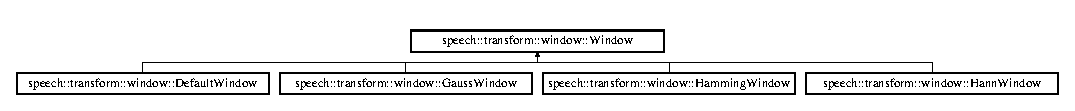
\includegraphics[height=1.040892cm]{classspeech_1_1transform_1_1window_1_1Window}
\end{center}
\end{figure}
\subsection*{Public Member Functions}
\begin{DoxyCompactItemize}
\item 
\hypertarget{classspeech_1_1transform_1_1window_1_1Window_a6c33bea81b0700d6d95d880ec985404a}{{\bfseries Window} (unsigned int window\+Size)}\label{classspeech_1_1transform_1_1window_1_1Window_a6c33bea81b0700d6d95d880ec985404a}

\item 
\hypertarget{classspeech_1_1transform_1_1window_1_1Window_a3e2b01bd3fe3722790b2c7023dfe0417}{double {\bfseries operator\mbox{[}$\,$\mbox{]}} (unsigned int index)}\label{classspeech_1_1transform_1_1window_1_1Window_a3e2b01bd3fe3722790b2c7023dfe0417}

\end{DoxyCompactItemize}
\subsection*{Protected Member Functions}
\begin{DoxyCompactItemize}
\item 
\hypertarget{classspeech_1_1transform_1_1window_1_1Window_acfb3c71e412b7aa1ba076c7f456717dd}{virtual const double {\bfseries get\+Window\+Multiplier} (unsigned int index)=0}\label{classspeech_1_1transform_1_1window_1_1Window_acfb3c71e412b7aa1ba076c7f456717dd}

\end{DoxyCompactItemize}


The documentation for this class was generated from the following files\+:\begin{DoxyCompactItemize}
\item 
/home/kacper/\+Projects/speech-\/recognition/src/speech/transform/window/Window.\+h\item 
/home/kacper/\+Projects/speech-\/recognition/src/speech/transform/window/Window.\+cpp\end{DoxyCompactItemize}

%--- End generated contents ---

% Index
\newpage
\phantomsection
\addcontentsline{toc}{chapter}{Index}
\printindex

\end{document}
